%!TEX encoding = UTF-8 Unicode
% !TeX spellcheck = en_GB
% Template to be used while publishing    
% a scientific work (PhD Thesis etc.)
% at the EDOC-Server of HU-Berlin                      
%    developed 2003-2008 by
% AG Elektronisches Publizieren, 
% Computer- und Medienservice,
% Humboldt-Universitaet zu Berlin
%    with friendly support of
% TeX-Stammtisch in Berlin     

% $Revision: 19 $
% $HeadURL: svn+ssh://ryckojox@svn.cms.hu-berlin.de/svn/projects/epub/latex/hudiss/mustermann.tex $
% $Date: 2009-07-03 15:49:19 +0200 (ptk, 03 lip 2009) $
% $Author$
% $Id: mustermann.tex 19 2009-07-03 13:49:19Z ryckojox $
                             
% Questions, comments, support:
%    edoc-latex@cms.hu-berlin.de    

% Documentation and information about the conditions of a publication:
%    http://edoc.hu-berlin.de/e_autoren/latex          

% Upload:
%    https://edoc.hu-berlin.de/cgi/dokupload/dokupload.cgi

%\documentclass[openright,twoside,headsepline]{scrbook}[2007/12/24]
\documentclass[openright,twoside,headsepline]{scrbook}
% The following package is necessary.
% To change the default options of the packages, use the key=value interface.
% See the documentation for details.
% If you need to use any special characters or LaTeX-commands 
% within the options, use \hudisssetup{} after loading this package,
% otherwise they will NOT work correctly.
\usepackage[
    inputenc=utf8, % default - latin1
    fontset=lmodern, % other possible parameters: lmodern, times, palatino
    %natbib={round,authoryear}, %include to use the natbib-package % sort sortiert nach Name
  %   jurabib={}, %include to use the jurabib-package
   %  apacite={}, %include to use the apacite-package
    hints=false, % set to 'false' for submission
    checktabu=false, % set to 'false' for submission
    draft=false, % set to 'false' for submission
    qserie=false
 ]{hudiss}
\newcommand{\citet}[1]{\cite{#1}}
\newcommand{\citep}[1]{\cite{#1}}
\newcommand{\citeauthor}[1]{\cite{#1}}

                
\hudisssetup{%
    titlepagefont={\Large\sffamily} % Use to change the titlepage font
}

% Fill out all the metadata here:
\hudissmetadata{%
    authorprefix={M.Sc.}, % e.g. Dipl.-Inf.
    authorfirstname={Lina}, % first name
    authorsurname={Alasfar}, % surname
    authorsuffix={}, % e.g. Ph.D.
    authoradd={geboren am 27.\,09.~1994 in Riad}, % date and place of birth
    doctitle={Phenomenology of the Higgs and Flavour Physics\\ In the Standard Model and Beyond}, % title of the thesis
    %docsubtitle={for one euro}, % subtitle of the thesis
    docsubject={Phenomenology of Elementary Particles}, % subject of the thesis (used in the properties of the pdf-document)
    approvala={Prof. Dr. R. Gr\"ober, Humboldt-Universit\"at zu Berlin}, % approvals: a-e
    approvalb={Prof. Dr. Dr. M. Musterman, Potsdam-Institut fur Klimafolgenforschung},
    approvalc={Prof. Dr. M. Mustermann2, Heidelberg},
    % approvald={},
    % approvale={},
    degree={doctor rerum naturalium\\(Dr. rer. nat.)}, % e.g. Dr. Rer. Nat.
    subject={Physik}, % e.g. Informatik
    faculty={Mathematisch-Wissenschaftlichen Fakult\"at}, % in Dativ/Genitiv! e.g. Mathematisch-Wissenschaftlichen Fakult\"at II
    university={Humboldt-Universit\"at zu Berlin}, % e.g. Humboldt-Universit\"at zu Berlin
    dean={Prof. Dr. Elmar Kulke}, % dean of the faculty
    president={Prof. Dr.-Ing. Dr. Sabine Kunst}, % president of the university
    datesubmitted={11. November 2013}, % the date of the submission
    dateexam={06. November 2013}, % the date of your last exam
    keywordsen={Complex Network, Epidemiology, Temporal Network, Statistical Physics}, % english keywords comma separated
    keywordsde={Komplexes Netzwerk, Epidemiologie Netzwerk, statistische Physik} % german keywords comma separated
}

% If you wish to load any further packages, 
% make any own adjustments (e. g. for the package fancyhdr)
% or define any own commands
% put ALL of them in the following file:
\KOMAoptions{numbers=noenddot}
\usepackage{amsmath,amssymb,amsfonts,amsthm,epigraph,scrpage2}
\usepackage[ngerman,english]{babel}
\usepackage{centernot} 
\usepackage{multirow,mathtools}
\usepackage{pdfpages}
\usepackage{currvita,geometry}
\renewcommand*{\cvheadingfont}{\large\bfseries} % CV Titel
\renewcommand*{\cvlistheadingfont}{\bfseries\sffamily} % sub-�berschriften
\renewcommand*{\cvlabelfont}{\sffamily} % items
\usepackage[compress,numbers,sort]{natbib}
\usepackage{placeins}
\usepackage{booktabs}
\usepackage{ragged2e}
\usepackage{etoolbox}
\usepackage{multirow}
\usepackage{amssymb}
\usepackage{bbold}
\usepackage{lieart}
\usepackage{booktabs,colortbl}
\usepackage{slashbox}
\usepackage[normalem]{ulem}
\usepackage{mathrsfs}
\usepackage{slashed,bbold}
%\usepackage{pict2e}
\usepackage{url}
\usepackage{multirow}
\usepackage{siunitx}
\usepackage{xcolor}
\usepackage{epigraph} 
\usepackage{rotfloat}
\usepackage[most]{tcolorbox}
%%%%%%%%%%%%%%%%%%%
% Colour Scheme
\definecolor{myblue}{HTML}{003366}
\usepackage{pgfplotstable}
\pgfplotsset{compat=1.8}
% see https://tex.stackexchange.com/a/60761/5001 for source of \breakingcomma
% (requires the "breqn" package; that's why it's loaded above)
\definecolor{rulecolor}{HTML}{003366}
\definecolor{tableheadcolor}{gray}{0.92}
% Following is taken from Werner: http://tex.stackexchange.com/a/33761/3061
% and modified for my needs
%
% Command \topline consists of a (slightly modified)
% \toprule followed by a \heavyrule rule of colour tableheadcolor
% (hence, 2 separate rules)
\newcommand{\toplinetwo}{ %
	\arrayrulecolor{rulecolor}\specialrule{0.1em}{\abovetopsep}{0pt}%
	\arrayrulecolor{white}\specialrule{\belowrulesep}{0pt}{0pt}%
	\arrayrulecolor{rulecolor}}

\newcommand{\topline}{ %
	\arrayrulecolor{rulecolor}\specialrule{0.1em}{\abovetopsep}{0pt}%
	\arrayrulecolor{tableheadcolor}\specialrule{\belowrulesep}{0pt}{0pt}%
	\arrayrulecolor{rulecolor}}
% Command \midline consists of 3 rules (top colour tableheadcolor, middle colour black, bottom colour white)
\newcommand{\midtopline}{ %
	\arrayrulecolor{tableheadcolor}\specialrule{\aboverulesep}{0pt}{0pt}%
	\arrayrulecolor{rulecolor}\specialrule{\lightrulewidth}{0pt}{0pt}%
	\arrayrulecolor{white}\specialrule{\belowrulesep}{0pt}{0pt}%
	\arrayrulecolor{rulecolor}}
% Command \bottomline consists of 2 rules (top colour
\newcommand{\bottomline}{ %
	\arrayrulecolor{white}\specialrule{\aboverulesep}{0pt}{0pt}%
	\arrayrulecolor{rulecolor} %
	\specialrule{\heavyrulewidth}{0pt}{\belowbottomsep}}%


\newcommand{\midheader}[2]{%
	\midrule\topmidheader{#1}{#2}}
\newcommand\topmidheader[2]{\multicolumn{#1}{c}{\textsc{#2}}\\%
	\addlinespace[0.5ex]}
%%%%%%%%%%%%%%%%%%%%%%%%%
\definecolor{Mahogany}{rgb}{0.36,0.54,0.66}
\definecolor{Cayenne}{rgb}{0.502,0.0,0.0}
\definecolor{Steel}{rgb}{0.4,0.4,0.4}
\definecolor{Tri_blue}{rgb}{0.039,0.5098,0.8}
\definecolor{Tri_yellow}{rgb}{0.5529,0.5451,0.0549}
\newcommand{\la}[1]{\textcolor{Cayenne}{#1}}
\definecolor{Gray}{gray}{0.95}
\newcommand{\CG}{\cellcolor{Gray}}
%\setcounter{secnumdepth}{3} % sub subsections numbering
%\setcounter{tocdepth}{3} % subsubsections inTOC

\usepackage[format=plain,singlelinecheck=false, font={sf,small},labelfont={bf,color=Steel}]{caption}
\DeclareCaptionLabelSeparator{cayenne_period}{\textcolor{Cayenne}{.} }
\captionsetup{labelsep=cayenne_period}

% Colors
\addtokomafont{chapter}{\color{Steel}}
\addtokomafont{section}{\color{Steel}}
\addtokomafont{subsection}{\color{Steel}}
\addtokomafont{subsubsection}{\color{Steel}}
\addtokomafont{paragraph}{\color{Steel}}
\addtokomafont{disposition}{\color{Steel}}
\addtokomafont{pagehead}{\color{Steel}}
\renewcommand{\pnumfont}{\color{Steel}} 
\addtokomafont{headsepline}{\color{Steel}} 
\pagestyle{scrheadings}

% Textcolor for chapters in TOC
\makeatletter
\let\stdl@chapter\l@chapter
\renewcommand*{\l@chapter}[2]{%
  \stdl@chapter{\textcolor{black}{#1}}{\textcolor{black}{#2}}}
\makeatother

%  labels in description environments
\renewcommand{\descriptionlabel}{\hspace\labelsep{}\sffamily\small\bfseries{}\color{Steel}{}}

%\makeatletter % dot after sections and all below
%\let\std@sect\@sect
%\def\@sect#1#2#3#4#5#6[#7]#8{\std@sect{#1}{#2}{#3}{#4}{#5}{#6}[#7.]{#8\color{Cayenne}{.}}}
%\makeatother
\usepackage{acronym}

\usepackage[leftcaption]{sidecap} % inner, outer,left,right
\sidecaptionvpos{figure}{t}

% Papiergr��e
%\setlength{\paperwidth}{21cm}
%\setlength{\paperheight}{25cm}
%\recalctypearea
%\usepackage[pass]{geometry}
%\usepackage[cross,a4,center]{crop}

%% Flattersatz
%\usepackage[document]{ragged2e} % Flattersatz
%\setlength{\RaggedRightParindent}{1em} % evtl. parskip


%% Sans Serif
%\usepackage{cmbright}
%\renewcommand{\familydefault}{\sfdefault}
%% Palatino
%\usepackage[sc]{mathpazo}
%\linespread{1.05}         % Palatino needs more leading (space between lines)
%\setkomafont{sectioning}{\normalcolor\bfseries} % Kapitel�berschriften

%%% Kapitel�berschriften: Mit gro�en Zahlen
%\usepackage{titlesec}
%\titleformat{\chapter}[display]
%{\bfseries\Large}
%{ %\Huge\textsc{\chaptertitlename} % f�r das Wort 'Kapitel'
%\hfill\fontsize{120}{70}\selectfont\color{lightgray}\textbf{\thechapter}}
%{-2ex}
%%{\filleft\fontsize{50}{70}\selectfont\scshape} % Kapit�lchen oder...
%{\filleft\fontsize{50}{70}\selectfont\textbf} % ...oder keine Kapit�lchen
%[\vspace{0ex}]
%
%%%% Part�berschriften
%\titleformat{\part}[display]
%{\bfseries\Large}
%{ %\Huge\textsc{\chaptertitlename} % f�r das Wort 'Kapitel'
%\hfill\fontsize{120}{70}\selectfont\color{lightgray}\textbf{\thepart}}
%{-2ex}
%{\filleft\fontsize{50}{70}\selectfont\scshape} % Kapit�lchen oder...
%%{\filleft\fontsize{50}{70}\selectfont\textbf} % ...oder keine Kapit�lchen
%[\vspace{0ex}]


\newcommand{\ER}{Erd\H{o}s-R\'enyi }
\newcommand{\BA}{Barab\'asi-Albert }
\newcommand{\mean}[1]{\left< #1 \right>}
\newcommand{\abs}[1]{\left| #1 \right|}
\newcommand{\norm}[1]{\lVert#1\rVert}
\newcommand{\mat}[1]{\mathbf{#1}}
\newcommand{\tgraph}{\mathcal{G}}

\theoremstyle{definition} % non-italic
\newtheorem{annahme}{Annahme} % braucht amsthm
\newtheorem{definition}{Definition}
\newtheorem{theorem}{Theorem}
\newtheorem{satz}{Satz}
\newtheorem{frage}{Frage}
%\input{watermarks/watermark.tex}
\DeclareMathOperator{\nnz}{nnz}

% + Graphicspath nach begin document

% aus Doi hyperref machen
%\newcommand*{\doi}[1]{\href{http://dx.doi.org/\detokenize{#1}}{doi: \detokenize{#1}}}



% Hyperlinks Setup
\hypersetup{
    unicode=false,          
    pdftoolbar=true,        
    pdfmenubar=true,        
    pdffitwindow=false,     
    pdfstartview={FitH},    
    pdftitle={Resurrecting bbh with kinematic shapes},
    pdfauthor={Lina Alasfar, Ramona Groeber, Christophe Grojean, Ayan Paul and Zhuoni Qian},
    pdfkeywords={Future Colliders} {dihiggs} {Machine Learning} {Shapley Values},
    pdfnewwindow=true,
    colorlinks=true,
    linkcolor=myblue,
    citecolor=myblue,
    filecolor=myblue,
    urlcolor=myblue,
    linktocpage=true
}
\newcommand{\SM}{\mathrm{SM}}
\newcommand{\NP}{\mathrm{NP}}
\newcommand{\hc}{\mathrm{h.c.}}
\newcommand{\MSbar}{\overline{\mathrm{MS}}}
%%%%%%%%%%%%%%%%%%%%%%%%%%%%%%%%%%%%%%%%
% autoref configuration
\renewcommand{\sectionautorefname}{section}
\renewcommand{\subsectionautorefname}{section}
\renewcommand{\appendixautorefname}{appendix}
\renewcommand{\tableautorefname}{table}
\renewcommand{\figureautorefname}{figure}
\def\equationautorefname~#1\null{Eq.\,(#1)\null}
\newcommand{\appendixref}[1]{\hyperref[#1]{appendix~\ref{#1}}}

%%%%%%def
%%%%%% def
\newcommand{\pt}{p_{\scriptscriptstyle T}}

\newcommand{\sssty}[1]{\scriptscriptstyle#1}

\newcommand{\be}{\begin{equation}}
	\newcommand{\ee}{\end{equation}}

\newcommand{\mt}{m_t}

\newcommand{\vev}[1]{\langle {#1} \rangle}
\newcommand{\lsim}{\lesssim}
\newcommand{\gsim}{\gtrsim}

\newcommand{\invab}{\si{\per \atto\barn}}
\newcommand{\femtobarn}{\si{\femto\barn}}
\newcommand{\nn}{\nonumber}
\newcommand{\perc}{\%}
\newcommand\sss{\scriptscriptstyle}

\newcommand{\gev}{\,\textrm{GeV}}
\newcommand{\mev}{\,\textrm{MeV}}
\newcommand{\pb}{\,\textrm{pb}}
\newcommand{\tev}{\,\textrm{TeV}}
\newcommand{\TO}{\rightarrow}


\newcommand{\gnote}[1]{\textbf{[G:} \textit{#1}\textbf{]}}
\newcommand{\rnote}[1]{\textbf{[R:}\textit{#1}\textbf{]}}
\newcommand{\ppgnote}[1]{\textbf{[PPG:}\textit{#1}\textbf{]}}
\newcommand{\tth}{t\bar{t}H}
\newcommand{\tthc}{\lambda_{\tth}}
\newcommand{\pptth}{pp\TO\tth}
\newcommand{\ggtth}{gg\TO\tth}
\newcommand{\qqtth}{q\bar{q}\TO\tth}
\newcommand{\qqtthg}{q\bar{q}\TO\tth g}
\newcommand{\qgtthq}{qg\TO\tth q}
\newcommand{\asa}[2]{\alpha_s^{#1}\alpha^{#2}}
\newcommand{\ord}[1]{\mathcal{O}{(#1)}}
\newcommand{\mh}{m_{ \sss h}}
\newcommand{\mz}{m_{ \sss Z}}
\newcommand{\dm}{\Delta_m}
\newcommand{\Gfer}{G_{ \sss F}}

%%%%%%%%%%%%%
%%%%%%%%%%%%%%%%%%%%%%%%%%%%% math %%%%%%%%%%%%%%%%%%%%%%%%%%%%%%%%
\def\vev#1{\left\langle #1\right\rangle}
\def\abs#1{\left| #1\right|}
\def\mod#1{\abs{#1}}
\def\Im{\mbox{Im}\,}
\def\Re{\mbox{Re}\,}
\def\Tr{\mbox{Tr}\,}
\def\det{\mbox{det}\,}
\def\etal{\hbox{\it et al.}}
\def\ie{\hbox{\it i.e.}{}}
\def\eg{\hbox{\it e.g.}{}}
\def\etc{\hbox{\it etc}{}}
%%%%%%%%%%%%%%%%%%%%%%%%%%%%%
\newcommand{\mr}[1]{\multirow{2}{*}{#1} }
\newcommand{\rb}[1]{\rotatebox{90}{#1}}
\newcommand{\neff}{n_{\rm eff}}
\renewcommand{\d}{{\rm d}}
\renewcommand{\bar}{\overline}
\newcommand{\hoppet}{\textsc{Hoppet}}
\newcommand{\R}[2]{$R_{#1#2}$}
%\newcommand{\as}{$\alpha_s$}
\newcommand{\rr}[1]{{\color{red}#1}}
\newcommand{\bb}[1]{{\color{blue}#1}}
\newcommand{\vs}{v_{\scriptscriptstyle S}}
\newcommand{\vh}{v_{\scriptscriptstyle H}}
\newcommand{\lambdah}{\lambda_{\scriptscriptstyle H}}
\newcommand{\muh}{\mu_{\scriptscriptstyle H}}
\newcommand{\LO}{\textrm{LO}}
\newcommand{\NLO}{\textrm{NLO}}
%%%%%%%%%%%%%

\DeclareOldFontCommand{\rm}{\normalfont\rmfamily}{\mathrm}
%\DeclareOldFontCommand{\sf}{\normalfont\sffamily}{\mathsf}
%\DeclareOldFontCommand{\tt}{\normalfont\ttfamily}{\mathtt}
\DeclareOldFontCommand{\bf}{\normalfont\bfseries}{\mathbf}
\DeclareOldFontCommand{\it}{\normalfont\itshape}{\mathit}
\DeclareOldFontCommand{\sl}{\normalfont\slshape}{\@nomath\sl}
\DeclareOldFontCommand{\sc}{\normalfont\scshape}{\@nomath\sc}
%\DeclareRobustCommand*\cal{\@fontswitch\relax\mathcal}
\DeclareRobustCommand*\mit{\@fontswitch\relax\mathnormal}

\def\abs#1{\left|#1\right|}

\newcommand{\bra}[1]{\mbox{$\langle\, #1 \mid$}}
\newcommand{\ket}[1]{\mbox{$\mid #1\,\rangle$}}
\newcommand\mydot{\!\cdot\!}
\newcommand\ep{\epsilon}
\newcommand\half{\frac{1}{2}}
\newcommand\quarter{\frac{1}{4}}
\newcommand\qb{\bar{q}}
\newcommand\ub{\bar{u}}
\newcommand\db{\bar{d}}
\newcommand\tb{\bar{t}}
\newcommand\sqs{\sqrt{s}}
\newcommand\epem{e^+e^-}
\newcommand\mpmm{\mu^+\mu^-}
\newcommand\irmv{\remove{i}{0.18}}
\newcommand\jrmv{\remove{j}{0.21}}
\newcommand\irmvb{\removeb{i}{0.18}{0.18}}
\newcommand\jrmvb{\removeb{j}{0.21}{0.17}}
\newcommand\isubrmv{\remove{i}{0.125}}
\newcommand\jsubrmv{\remove{j}{0.145}}
\newcommand\FKSpairs{{\cal P}_{\sss\rm FKS}}
\newcommand\FKSpairsred{\overline{{\cal P}}_{\sss\rm FKS}}
\newcommand\FKSelem{N_{\sss\rm FKS}}
\newcommand\FKSelemred{\overline{N}_{\sss\rm FKS}}
\newcommand\nchannels{N_{\rm ch}}
\newcommand\proc{\qqtth}
\newcommand\procB{r_{\sss B}}
\newcommand\procR{r_{\sss R}}
\newcommand\allproc{{\cal R}}
\newcommand\allprocnpo{\allproc_{n+1}}
\newcommand\allprocn{\allproc_{n}}
\newcommand\BornME{{\cal B}}
\newcommand\nini{n_{\sss I}}
\newcommand\nlight{n_{\sss L}}
\newcommand\nlightB{\nlight^{\sss (B)}}
\newcommand\nlightR{\nlight^{\sss (R)}}
\newcommand\nlightBorR{\nlight^{\sss (B/R)}}
\newcommand\nheavy{n_{\sss H}}
\newcommand\nzero{n_\emptyset}
\newcommand\ident{{\cal I}}
\newcommand\numofgr{N_d}
\newcommand\amp{{\cal A}}
\newcommand\ampmt{\amp^{(m,0)}}
\newcommand\ampnt{\amp^{\asa{1}{1/2}}}
\newcommand\ampntb{\amp^{\alpha^{3/2}}}
\newcommand\ampnpot{\amp^{\asa{3/2}{1/2}}}
\newcommand\ampnpotb{\amp^{\asa{1/2}{3/2}}}
\newcommand\ampnl{\amp_{\proc,~\text {Loop}}^{\asa{2}{1/2}}}
\newcommand\ampnlb{\amp_{\proc,~\text {Loop}}^{\asa{1}{3/2}}}
\newcommand\ampsq{{\cal M}}
\newcommand\ampsqmt{\ampsq^{(m,0)}}
\newcommand\ampsqnt{\ampsq^{(n,0)}}
\newcommand\ampsqnpot{\ampsq^{(n+1,0)}}
\newcommand\ampsqnl{\ampsq^{(n,1)}}
\newcommand\vampsqnl{{\cal V}^{(n,1)}}
\newcommand\hvampsqnl{\hat{\cal V}^{(n,1)}}
\newcommand\vampsqnlF{{\cal V}^{(n,1)}_{\sss FIN}}
\newcommand\hvampsqnlF{\hat{\cal V}^{(n,1)}_{\sss FIN}}
\newcommand\tampsq{\widetilde{\cal M}}
\newcommand\tampsqnt{\tampsq^{(n,0)}}
\newcommand\tampsqnpot{\tampsq^{(n+1,0)}}
\newcommand\rone{r_{[1]}}
\newcommand\rtwo{r_{[2]}}
\newcommand\Ione{\ident_1}
\newcommand\Itwo{\ident_2}
\newcommand\xii{\xi_i}
\newcommand\yij{y_{ij}}
\newcommand\phii{\varphi_i}
\newcommand\yi{y_i}
\newcommand\xic{\left(\frac{1}{\xii}\right)_c}
\newcommand\lxic{\left(\frac{\log\xii}{\xii}\right)_c}
\newcommand\omyijd{\left(\frac{1}{1-\yij}\right)_\delta}
\newcommand\omyid{\left(\frac{1}{1-\yi}\right)_\delta}
\newcommand\opyid{\left(\frac{1}{1+\yi}\right)_\delta}
\newcommand\Dfun{{\cal D}}
\newcommand\Sfun{{\cal S}}
\newcommand\Sfunij{\Sfun_{ij}}
\newcommand\asfun{a_{\Sfun}}
\newcommand\bsfun{b_{\Sfun}}
\newcommand\stepf{\Theta}
\newcommand\phsp{d\phi}
\newcommand\phspn{\phsp_{n}}
\newcommand\phspnpo{\phsp_{n+1}}
\newcommand\tphsp{d\widetilde{\phi}}
\newcommand\tphspn{\tphsp_{n}}
\newcommand\tphspnij{\tphsp_{n}^{ij}}
\newcommand\asotwopi{\frac{\as}{2\pi}}
\newcommand\gs{g_{\sss S}}
\newcommand\aW{\alpha_{\sss W}}
\newcommand\gW{g_{\sss W}}
\newcommand\aem{\alpha}
\newcommand\xicut{\xi_{cut}}
\newcommand\ximax{\xi_{\rm max}}
\newcommand\deltaO{\delta_{\sss O}}
\newcommand\deltaI{\delta_{\sss I}}
\newcommand\NC{N_{\sss c}}
\newcommand\CA{c_{\sss A}}
\newcommand\CF{c_{\sss F}}
\newcommand\TF{T_{\sss F}}
\newcommand\DA{D_{\sss A}}
\newcommand\eikint{{\cal E}}
\newcommand\eikintD{\hat{\cal E}}
\newcommand\APdamp{\overline{P}}
\newcommand\Qdamp{\overline{Q}}
\newcommand\Qop{\vec{Q}}
\newcommand\JetsB{J^{\nlightB}}
\newcommand\JetsR{J^{\nlightB+1}}
\newcommand\kin{\left\{k_k\right\}}
\newcommand\velkl{v_{kl}}
\newcommand\alkl{\alpha_{kl}}
\newcommand\avg{{\cal N}}
\newcommand\symm{\varsigma}
\newcommand\symmnij{\symm_{ij}^{(n)}}
\newcommand\symmnpoij{\symm_{ij}^{(n+1)}}
\newcommand\veck{\vec{k}}
\newcommand\kbar{\bar{k}}
\newcommand\kkdotkl{k_k\mydot k_l}
\newcommand\polv{\varepsilon}
\newcommand\polP{{\cal T}}
\newcommand\polQ{{\cal W}}
\newcommand\muF{\mu_{\sss F}}
\newcommand\muR{\mu_{\sss R}}
\newcommand\clH{{\mathbb H}}
\newcommand\clS{{\mathbb S}}
\newcommand\bt{\bar{t}}
\newcommand\bq{\bar{q}}
\newcommand\bqp{\bar{q}^\prime}
\newcommand\aNLO{{\sc\small MadGraph5\_aMC@NLO}}
\newcommand\UFO{{\sc\small UFO}}
\newcommand\MLf{{\sc\small MadLoop5}}
\newcommand\ML{{\sc\small MadLoop}}
\newcommand\CutTools{{\sc\small CutTools}}
\newcommand\OL{{\sc\small OpenLoops}}
\newcommand\MadFKS{{\sc\small MadFKS}}
\newcommand{\Ht}{H_{\sss T}}
\newcommand{\GeV}{\si{\GeV}}
\newcommand{\TeV}{\si{\TeV}}
%\newcommand{\invab}{\si{\per \atto\barn}}
 \newcommand{\ght}{g_{h t \bar t}}
\newcommand{\ghht}{g_{hh t \bar t}}
\newcommand{\cuh}{ C_{t\phi} }
\newcommand{\cbh}{ C_{b\phi}}
\newcommand{\cqu}{C_{Qt}}
\newcommand{\cquqd}{C_{QtQb}}
\newcommand{\eps}{\epsilon}
\newcommand{\as}{\frac{\alpha_s^0}{4 \pi} }
\newcommand{\Zas}{ Z_{\alpha_s} }
\newcommand{\asr}{\frac{\alpha_s}{4 \pi} }
\newcommand{\Red}[1]{{\color{nicered}{#1}}}
%%%%%%%%%%%%% functions for eff  %%%%%%%%%%%
% short-hands
\newcommand*{\mg}{\texttt{MG5\_aMC@NLO}}
\newcommand*{\fb}{\text{fb}}
\newcommand*{\iab}{\ensuremath{\text{ab}^{-1}}}
\DeclareMathOperator*{\cov}{cov}
\newcommand{\inab}{\,{\rm ab}^{-1}}
\newcommand{\infb}{\,{\rm fb}^{-1}}
\newcommand{\bbh}{b\bar bh}
\newcommand{\ggh}{gg\to h}
\newcommand{\bbaa}{b\bar b\gamma\gamma}
\newcommand{\tkab}{\tilde{\kappa}_b}
\newcommand{\kab}{\kappa_b}
\DeclareMathOperator{\BR}{BR}
\newcommand{\La}{\mathcal{L} }
\newcommand{\hhbox}{hh^{gg\rm F}_{\rm box}}
\newcommand{\hhtri}{hh^{gg\rm F}_{\rm tri}}
\newcommand{\hhint}{hh^{gg\rm F}_{\rm int}}
\newcommand{\qqA}{q\bar q \rm A}
\newcommand{\uuA}{u\bar u \rm A}
\newcommand{\ddA}{d\bar d \rm A}
\newcommand{\QQh}{Q\bar Q h}
\newcommand{\HEPfit}{\texttt{HEPfit}}

%%Maths stuff 
\newcommand{\parenths}[1]{\left({#1}\right)\xspace}
\newcommand{\braces}[1]{\left\{{#1}\right\}\xspace}
\newcommand{\sqbracs}[1]{\left[{#1}\right]\xspace}
\newcommand{\colvector}[1]{\begin{pmatrix}#1\end{pmatrix}\xspace}
\newcommand{\expec}[1]{\langle #1\rangle}
\newcommand{\Zp}{Z^\prime}
\newcommand{\s}{\hat{s}}
% number of expected events theoretical 289
%%%
\def\beq{\begin{equation}}
	\def\bea{\begin{eqnarray}}
		\def\eeq{\end{equation}}
	\def\eea{\end{eqnarray}}
\def\beqnl{\begin{align}}
	\def\endal{\end{align}}

%\usepackage[T1]{fontenc}
%
% The order of the parts in the document is only our suggestion,
% you can change it, if you wish.
% Don't put any other text between those commands.
% Do not remove the \*matter macros.
% Use standard macros to include new chapters.



%%%%%    \includeonly{chapters/Part1/01-Introtext}
% DIV is 10, BCOR is 0mm
\begin{document}
\graphicspath{./figures/}

\selectlanguage{english}
    \frontmatter
    	%\includepdf{Thesis_Cover.pdf}
	%\cleardoublepage
        \maketitle
        \cleardoublepage
        %\cleardoublepage

\null\vfill\itshape

\begin{flushright}
	Ich widme diese Arbeit \\
	meiner Familie und meinen Freunden
\end{flushright}
\thispagestyle{empty}
\upshape\cleardoublepage


       %!TEX encoding = UTF-8 Unicode
% !TeX spellcheck = en_GB

\selectlanguage{english}
\begin{abstract}
This thesis investigates some aspects for the future of Higgs measurements after a decade of its discovery, focusing on the potential for the future runs of the Large Hadron Collider. \\ The first part provides  an overview of the Higgs theory and measurements, with some meta-analysis on the most recent results and focus on the Standard Model Effective Field theory~(SMEFT). The second part is concerned with single-Higgs production, and two-loop calculation of $Zh$ production via gluon fusion. Then a SMEFT analysis of the interplay between Higgs self-coupling and four heavy quark operators stemming from Higher order effects. \\ The third part focuses on the Higgs pair production, an essential process for measuring Higgs-self coupling. Employing multivariate analysis to study its potential for probing light Yukawa couplings.\\ Lastly, some models aims to explain the recent flavour anomalies are proposed, in the light of a global SMEFT Bayesian analysis. 

\paragraph{Keywords\color{Cayenne}{:}} Higgs Physics, Standard Model Effective Field Theory, Flavour observables, Statistical data analysis.
\end{abstract}

%\cleardoublepage


\selectlanguage{ngerman}
\begin{abstract}
Diese Dissertation untersucht einige Aspekte für die Zukunft der Higgs-Messungen nach einem Jahrzehnt seiner Entdeckung, im Rahmen der Zukunft des LHC's\\ Der erste Teil bietet einen Überblick über die Higgsphysik und -Messungen, mit einigen Metaanalysen zu den aktuellen Ergebnissen und einem Schwerpunkt auf der Standardmodell-Effektivfeld-Theorie (SMEFT). Der zweite Teil befasst sich mit der Einzel-Higgs-Produktion.  Zusätzlich werden Ergebnisse für $Zh$-Produktion via Gluon-Fusion in nächstführender Ordnung in der starken Kopplungskonstante im Niederenergielimes präsentiert. Dann eine SMEFT-Analyse der Interaktion zwischen Higgsselbstkopplung und vier Heavy-Quark-Operatoren, die von Korrekturen höherer Ordnung stammen. \\ Der dritte Teil konzentriert sich auf die Higgspaarproduktion, ein wesentlicher Prozess zur Messung der Higgsselbstkopplung. Unter Verwendung multivariater Analyse zur Untersuchung seines Potenzials zur Untersuchung leichter Yukawa-Kopplungen. \\ Schließlich werden einige Modelle vorgeschlagen, um die letzten Flavour-Anomalies im inspiriert von einer globalen SMEFT-Bayesschen Analyse zu erklären.
%\vspace{-0.2cm}
%\vfill
\paragraph{Schlagw\"orter\color{Cayenne}{:}} Higgs Physik, Standardmodell-Effektivfeld-Theorie,  Flavour Anomalies, Statistische Datenanalyse
\end{abstract}

% Back to main language
\selectlanguage{english}
\cleardoublepage
        \tableofcontents    
         %!TEX encoding = UTF-8 Unicode
% !TeX spellcheck = en_GB
%\chapter*{}
\section*{List of abbreviations}
%\addcontentsline{toc}{chapter}{List of abbreviations}
%\thispagestyle{plain}
\begin{acronym}[nnzzzzzzz] %5 l�ngste Abk�rzung ineckigen Klammern zur Ausrichtung
%\setlength{\itemsep}{-\parsep}
\acro{}[\color{Steel}{Colliders and working groups }\color{Cayenne}{.}]{}
\acro{CERN}{ Conseil europ\'een pour la recherche nucl\'eaire.}
\acro{LHC}{Large Hadron Collider}
\acro{HL-LHC}{High-Luminosity LHC}
\acro{CMS}{Compact Muon Solenoid}
\acro{ATLAS}{A Toroidal LHC ApparatuS}
\acro{LEP}{Large Electron-Positron Collider}
\acro{ALEPH}{Apparatus for LEp PHysics}
\acro{SLC}{Stanford Linear Collider}
\acro{FCC}{Future circular collider}
\acro{HXSWG}{Higgs cross-section working group}
\acro{PDG}{Particle data group}
\acro{}[\color{Steel}{Higgs and Standard Model physics}\color{Cayenne}{.}]{}
\acro{SM}{ Standard Model}
\acro{QCD}{ Quantum chromodynamics}  
\acro{QED}{ Quantum electrodynamics}  
\acro{EFT}{ Effective field theory}
\acro{SMEFT}{ Standard Model effective field theory}
\acro{HEFT}{ Higgs effective field theory}
\acro{EW}{Electroweak}
\acro{VEV/ vev}{Vacuum expectation value}
\acro{EWSB}{Electroweak symmetry breaking}
\acro{EWPO}{Electroweak precision observables}
\acro{EWChL}{Electroweak chiral Lagrangian}
\acro{SSB}{Spontanious symmetry breaking} 
\acro{SU}[$SU(N)$]{Special unitary (group) of dimension $N$}
\acro{ggF}{Gluon fusion (processes)}
\acro{qqA}[$\qqA$]{Quark anti-quark anhitation (processes) }
\acro{PDF}{Parton distribution functions}
\acro{STXS}{Simplified template cross-sections}
\acro{}[\color{Steel}{Higher order computations}\color{Cayenne}{.}]{}
\acro{RGE}{Renormalisation group equation or evolution} 
\acro{LO, NLO ...}{Leading order, Next to leading order etc.} 
\acro{HTL}{Heavy top limit }   
\acro{HPL}{Harmonic polylogarithms}   
\acro{GPL}{Generalised polylogarithms }   
\acro{}[\color{Steel}{Flavour}\color{Cayenne}{.}]{}
\acro{CKM}{Cabibbo-Kobayashi-Maskawa-Matrix}
\acro{CP}[$\mathcal{CP}$]{Charge conjugation and parity}  
\acro{MFV}{Minimal flavour violation}  
\acro{AFV}{Aligned flavour violation}
\acro{SFV}{Spontanious flavour violation}
\acro{PDD}{Phenomenological data-driven}  
\acro{PMD}{Phenomenological model-driven}
\acro{FCNC}{Flavour-changing neutral currents}  
\acro{LUV}{Lepton universality violation}  
\acro{}[\color{Steel}{Data analysis/statistics}\color{Cayenne}{.}]{}
\acro{MC}{Monte Carlo (simulation)}
\acro{ML}{Machine learning}
\acro{BDT}{Boosted decision tree}
\acro{XGBoost}{EXtreme gradient boosted decision tree}   
\acro{DNN}{Deep Neural Networks}
\acro{MCMC}{Markov chain Monte Carlo (Bayesian analysis)}
\acro{PCo}{Principle component}
\acro{FDR}{False discovery rate}
\acro{ANOVA}{Analysis of variation}
\acro{}[\color{Steel}{New Physics}\color{Cayenne}{.}]{}
\acro{4F}{Four-fermion}
\acro{NP}{New physics}
\acro{BSM}{Beyond the Standard Model}
\acro{VLQ}{Vector-like quarks}
\acro{LQ}{Leptoquarks}
\acro{2HDM}{Two-Higgs-doublet model}
\acro{CHM}{Composite Higgs model}
\acro{MSSM}{Minimal supersymmetric Standard Model}
\acro{SILH}{Strongly interacting light Higgs}
\end{acronym}

    \mainmatter
        % Part 0
        %%!TEX encoding = UTF-8 Unicode
% !TeX spellcheck = en_GB


\chapter{Introduction}
\par The discovery of the Higgs boson in 2012 by the ATLAS~\cite{ATLAS:2012yve}  and CMS~\cite{CMS:2012qbp} experiments at the {L}arge {H}adron {C}ollider~(LHC) marks the completion of the Standard Model of particle physics~(SM)~\cite{salam1,salam2,PhysRevLett.19.1264}; as it was a direct prediction of the spontaneous symmetry breaking mechanism observed in the SM~\cite{PhysRevLett.13.321,PhysRevLett.13.508,HIGGS1964132,PhysRevLett.13.585,Guralnik:2009jd}. However, this discovery has brought more questions than answers, and even after a decade of its discovery, there is a lot to know about this particle and its potential connections with physics beyond the SM.

\par Understanding the properties and couplings of the Higgs boson has become the preeminent goal of the LHC. Higgs measurements are getting progressively accurate, and our understanding of this particle is approaching a few per cent-level. The future runs of the LHC will open the doors to the Higgs-precision era. However, increased luminosity, i.e. data acquisition from the LHC, without improving the theoretical prediction of Higgs processes is futile. Therefore, to ensure the success of the experimental efforts in probing Higgs couplings and properties at the required precision, it is imperative to include higher-order calculations for Higgs production cross-sections. \\ 
An example of such processes is the associated production of the Higgs boson with a $Z$ boson, which suffers from higher theoretical uncertainties than its sister process, the $Wh$ production, because it contains a gluon fusion sub-process $ gg \to Zh$. Furthermore, the gluon fusion channel generally tends to have large higher-order corrections compared to the quark-initiated one;  thereby, prompting the need to compute its higher order corrections, in order to improve the theoretical prediction of  $Zh$ production. Such computation can be carried out efficiently using a state-of-the-art analytic technique based on the expansion in small transverse momentum proposed in ref.~\cite{Bonciani:2018omm}. 
%
 \par After a decade of \emph{Higgs physics}, and over ten-thousand Higgs-related publications, we still have a lot to learn about the Higgs boson.  In particular, its potential structure is yet to be probed experimentally, and so are its couplings to the light quarks and leptons. Measurements of Higgs self-coupling will reveal if there are, for instance, new scalars beyond the Higgs boson that we have not yet directly observed. Furthermore, studying Higgs coupling to light fermions is essential in understanding the source of their masses' origin and explaining the significant hierarchy between these across the three generations of matter. 
%The High Energy Physics community anticipated that the Higgs discovery, especially given its mass is $ m_h <130$ GeV, will be followed by the detection of a \emph{Zoo} of particles stemming from the Supersymmetric extension of the SM. Unfortunately, this was not the case, and we have not seen any new particles discovered after the Higgs boson. 
\par The conclusion of the SM-related discoveries did not leave any specific hints to the nature and scale of new physics~(NP).  Moreover, many experimental searches have excluded NP at scale close to the electroweak symmetry breaking, for most recent searches cf.~\cite{ATLAS-CONF-2022-006,ATLAS-CONF-2022-011,ATLAS-CONF-2022-012,ATLAS-CONF-2022-010,ATLAS-CONF-2022-009,CMS-PAS-EXO-20-011,CMS-PAS-EXO-21-010,CMS-PAS-EXO-21-003,CMS-PAS-EXO-20-006,CMS-PAS-EXO-21-006,CMS:2022nty,CMS:2022yjm}. Although NP is needed to explain the shortcomings of the SM as for instance: neutrino masses, or give a candidate for dark matter and so on. Experimental searches have excluded for most scenarios that NP is at a scale close to the electroweak symmetry breaking.
This motivates parametrising NP effects in a model-independent manner, in terms of higher-dimensional operators suppressed by some high scale~$\Lambda$ . This formalism is known as the Standard Model Effective Field Theory~(SMEFT) framework~\cite{Giudice:2007fh,Grzadkowski:2010es,Contino:2013kra, Elias-Miro:2013eta,Gupta:2014rxa}. In SMEFT, all leading NP effects in Higgs physics are summarised in a numerable set of mass dimension six operators, that makes minimal assumptions about the nature of NP, guaranteeing a model-independent approach to collider searches.
The use of SMEFT in higher-order calculations of Higgs rates has revealed insights into the Higgs potential by the appearance of the Higgs trilinear self-coupling within electroweak loop corrections of single-Higgs processes. This allows to put constraint on this coupling from measurements of single-Higgs rates at the LHC can be used to constrains this coupling~\cite{McCullough:2013rea, Gorbahn:2016uoy, Degrassi:2016wml, Bizon:2016wgr, Maltoni:2017ims, Degrassi:2019yix, Degrassi:2021uik, Haisch:2021hvy}. Nevertheless, more SMEFT operators can also enter in single-Higgs loops that alter the constraining power of these measurements. The interconnectivity between the Higgs and top-quark sectors is  emphasised within the SMEFT framework, as recent global fits have established strong correlations between observables from both sectors as well as the electroweak precision observables~(EWPO)~\cite{Ellis:2020unq}. Strong correlations between the top sector and EWPO are also seen at loop-level~\cite{Dawson:2020oco,Dawson:2022bxd} thus; one expects to see similar correlations emerging from loop effects of top operators on Higgs processes.
\par The observation of Higgs pairs is slated for the High-Luminosity (HL) LHC operating phase. This rare process will be --if observed-- the {\it pi\`ece de r\'esistance} of the LHC Higgs physics programme~\cite{Bernius:2666331}, directly measuring the Higgs trilinear self-interaction, also untangling Higgs potential measurements from the top-sector interactions. Furthermore,  this process could be of great utility in probing Higgs coupling to light quarks, from the enhancement of the quark-initiated Higgs pair production, cf.~\cite{Alasfar:2019pmn,Egana-Ugrinovic:2021uew} and as will be shown in this thesis.  The full potential of Higgs pair production can be exploited when it is treated as a multivariate problem by implementing an interpretable machine learning analysis technique~\cite{Grojean:2020ech}. In this manner, it is possible to have  simultaneous constraints of the two most elusive Higgs interactions, light-quark Yukawa and the trilinear couplings.
\par Recent measurements, by Belle and Babar, in addition to the LHCb experiment at CERN, of $B$-mesons semi-leptonic decays showed some tension with the SM predictions of lepton flavour universality of electroweak couplings~\cite{Aaij:2014ora,Aaij:2017vbb,Aaij:2019wad,Abdesselam:2019wac,LHCb:2021trn}, with up to $\sim 3\sigma$ deviation from the SM~\cite{Chatrchyan:2013bka,Aaij:2017vad,Aaboud:2018mst,Aaij:2020nol}. These anomalies require models with some flavour violation that makes model-building for explaining these anomalies at tree-level  Augean task~\cite{DiLuzio:2017vat,Calibbi:2017qbu,Bordone:2017bld,Barbieri:2017tuq,Assad:2017iib,Heeck:2018ntp,Fornal:2018dqn,Crivellin:2018yvo,Crivellin:2019dwb,Bordone:2019uzc}. Additionally, to complicate things further, these anomalies are in tension with EWPO. Hence, this thesis promotes a more careful treatment of these anomalies, by introducing them at the loop level in SMEFT and performing a global fit combining both flavour and EWPO data. The fit result would allow for a SMEFT guided UV-model building for these anomalies, with extended Higgs and top sectors. 
\paragraph{This thesis is structured as follows\color{Cayenne}{:}}
I start by presenting the basics of Effective Fields Theories relevant to Higgs physics at the LHC in~\autoref{chap:HiggsEFT}. \\ The second part of the thesis focuses on the production of --single-- Higgs at the LHC, starting with an overview in~\autoref{chap:overviewSingleHiggs}, followed by a discussion on the use of the $\pt$-expansion technique for obtaining an analytic expression for the virtual correction of the gluon fusion $Zh$ production in~\autoref{chap:hz}. Next, \autoref{chap:4topSingleHiggs} showcases the potential of single-Higgs processes to probe four-fermion operators from the top sector, by performing higher-order computations of these processes in SMEFT. The potential for constraining these operators for the considered single-Higgs production processes alongside the trilinear Higgs self-coupling is investigated by means of a Bayesian fit. \\ The third part of the thesis focuses on the production of Higgs boson in pairs at the HL-LHC~(\autoref{chap:overviewDiHiggs}). Afterwards, in~\autoref{chap:lightyuk}, I show the potential for employing Higgs pair production to probe light quark couplings to the Higgs boson. In addition, I show a multivariate analysis method, that maximises the efficiency of extracting the Higgs pair signal using interpretable machine learning.  The last part of the thesis, \autoref{chap:flav}, describes the potential UV models for the $B$ anomalies, inspired by a global SMEFT fit and minimal flavour violation~(MFV). 










        %%\documentclass[openright,twoside,headsepline]{scrbook}
%\usepackage[applemac]{inputenc}
%\usepackage{graphicx,xcolor,hyperref} % obsolete in HU-diss
%\usepackage[round,authoryear]{natbib}
%\setlength\bibhang{2em} 
%
%
%\KOMAoptions{numbers=noenddot}
\usepackage{amsmath,amssymb,amsfonts,amsthm,epigraph,scrpage2}
\usepackage[ngerman,english]{babel}
\usepackage{centernot} 
\usepackage{multirow,mathtools}
\usepackage{pdfpages}
\usepackage{currvita,geometry}
\renewcommand*{\cvheadingfont}{\large\bfseries} % CV Titel
\renewcommand*{\cvlistheadingfont}{\bfseries\sffamily} % sub-�berschriften
\renewcommand*{\cvlabelfont}{\sffamily} % items
\usepackage[compress,numbers,sort]{natbib}
\usepackage{placeins}
\usepackage{booktabs}
\usepackage{ragged2e}
\usepackage{etoolbox}
\usepackage{multirow}
\usepackage{amssymb}
\usepackage{bbold}
\usepackage{lieart}
\usepackage{booktabs,colortbl}
\usepackage{slashbox}
\usepackage[normalem]{ulem}
\usepackage{mathrsfs}
\usepackage{slashed,bbold}
%\usepackage{pict2e}
\usepackage{url}
\usepackage{multirow}
\usepackage{siunitx}
\usepackage{xcolor}
\usepackage{epigraph} 
\usepackage{rotfloat}
\usepackage[most]{tcolorbox}
%%%%%%%%%%%%%%%%%%%
% Colour Scheme
\definecolor{myblue}{HTML}{003366}
\usepackage{pgfplotstable}
\pgfplotsset{compat=1.8}
% see https://tex.stackexchange.com/a/60761/5001 for source of \breakingcomma
% (requires the "breqn" package; that's why it's loaded above)
\definecolor{rulecolor}{HTML}{003366}
\definecolor{tableheadcolor}{gray}{0.92}
% Following is taken from Werner: http://tex.stackexchange.com/a/33761/3061
% and modified for my needs
%
% Command \topline consists of a (slightly modified)
% \toprule followed by a \heavyrule rule of colour tableheadcolor
% (hence, 2 separate rules)
\newcommand{\toplinetwo}{ %
	\arrayrulecolor{rulecolor}\specialrule{0.1em}{\abovetopsep}{0pt}%
	\arrayrulecolor{white}\specialrule{\belowrulesep}{0pt}{0pt}%
	\arrayrulecolor{rulecolor}}

\newcommand{\topline}{ %
	\arrayrulecolor{rulecolor}\specialrule{0.1em}{\abovetopsep}{0pt}%
	\arrayrulecolor{tableheadcolor}\specialrule{\belowrulesep}{0pt}{0pt}%
	\arrayrulecolor{rulecolor}}
% Command \midline consists of 3 rules (top colour tableheadcolor, middle colour black, bottom colour white)
\newcommand{\midtopline}{ %
	\arrayrulecolor{tableheadcolor}\specialrule{\aboverulesep}{0pt}{0pt}%
	\arrayrulecolor{rulecolor}\specialrule{\lightrulewidth}{0pt}{0pt}%
	\arrayrulecolor{white}\specialrule{\belowrulesep}{0pt}{0pt}%
	\arrayrulecolor{rulecolor}}
% Command \bottomline consists of 2 rules (top colour
\newcommand{\bottomline}{ %
	\arrayrulecolor{white}\specialrule{\aboverulesep}{0pt}{0pt}%
	\arrayrulecolor{rulecolor} %
	\specialrule{\heavyrulewidth}{0pt}{\belowbottomsep}}%


\newcommand{\midheader}[2]{%
	\midrule\topmidheader{#1}{#2}}
\newcommand\topmidheader[2]{\multicolumn{#1}{c}{\textsc{#2}}\\%
	\addlinespace[0.5ex]}
%%%%%%%%%%%%%%%%%%%%%%%%%
\definecolor{Mahogany}{rgb}{0.36,0.54,0.66}
\definecolor{Cayenne}{rgb}{0.502,0.0,0.0}
\definecolor{Steel}{rgb}{0.4,0.4,0.4}
\definecolor{Tri_blue}{rgb}{0.039,0.5098,0.8}
\definecolor{Tri_yellow}{rgb}{0.5529,0.5451,0.0549}
\newcommand{\la}[1]{\textcolor{Cayenne}{#1}}
\definecolor{Gray}{gray}{0.95}
\newcommand{\CG}{\cellcolor{Gray}}
%\setcounter{secnumdepth}{3} % sub subsections numbering
%\setcounter{tocdepth}{3} % subsubsections inTOC

\usepackage[format=plain,singlelinecheck=false, font={sf,small},labelfont={bf,color=Steel}]{caption}
\DeclareCaptionLabelSeparator{cayenne_period}{\textcolor{Cayenne}{.} }
\captionsetup{labelsep=cayenne_period}

% Colors
\addtokomafont{chapter}{\color{Steel}}
\addtokomafont{section}{\color{Steel}}
\addtokomafont{subsection}{\color{Steel}}
\addtokomafont{subsubsection}{\color{Steel}}
\addtokomafont{paragraph}{\color{Steel}}
\addtokomafont{disposition}{\color{Steel}}
\addtokomafont{pagehead}{\color{Steel}}
\renewcommand{\pnumfont}{\color{Steel}} 
\addtokomafont{headsepline}{\color{Steel}} 
\pagestyle{scrheadings}

% Textcolor for chapters in TOC
\makeatletter
\let\stdl@chapter\l@chapter
\renewcommand*{\l@chapter}[2]{%
  \stdl@chapter{\textcolor{black}{#1}}{\textcolor{black}{#2}}}
\makeatother

%  labels in description environments
\renewcommand{\descriptionlabel}{\hspace\labelsep{}\sffamily\small\bfseries{}\color{Steel}{}}

%\makeatletter % dot after sections and all below
%\let\std@sect\@sect
%\def\@sect#1#2#3#4#5#6[#7]#8{\std@sect{#1}{#2}{#3}{#4}{#5}{#6}[#7.]{#8\color{Cayenne}{.}}}
%\makeatother
\usepackage{acronym}

\usepackage[leftcaption]{sidecap} % inner, outer,left,right
\sidecaptionvpos{figure}{t}

% Papiergr��e
%\setlength{\paperwidth}{21cm}
%\setlength{\paperheight}{25cm}
%\recalctypearea
%\usepackage[pass]{geometry}
%\usepackage[cross,a4,center]{crop}

%% Flattersatz
%\usepackage[document]{ragged2e} % Flattersatz
%\setlength{\RaggedRightParindent}{1em} % evtl. parskip


%% Sans Serif
%\usepackage{cmbright}
%\renewcommand{\familydefault}{\sfdefault}
%% Palatino
%\usepackage[sc]{mathpazo}
%\linespread{1.05}         % Palatino needs more leading (space between lines)
%\setkomafont{sectioning}{\normalcolor\bfseries} % Kapitel�berschriften

%%% Kapitel�berschriften: Mit gro�en Zahlen
%\usepackage{titlesec}
%\titleformat{\chapter}[display]
%{\bfseries\Large}
%{ %\Huge\textsc{\chaptertitlename} % f�r das Wort 'Kapitel'
%\hfill\fontsize{120}{70}\selectfont\color{lightgray}\textbf{\thechapter}}
%{-2ex}
%%{\filleft\fontsize{50}{70}\selectfont\scshape} % Kapit�lchen oder...
%{\filleft\fontsize{50}{70}\selectfont\textbf} % ...oder keine Kapit�lchen
%[\vspace{0ex}]
%
%%%% Part�berschriften
%\titleformat{\part}[display]
%{\bfseries\Large}
%{ %\Huge\textsc{\chaptertitlename} % f�r das Wort 'Kapitel'
%\hfill\fontsize{120}{70}\selectfont\color{lightgray}\textbf{\thepart}}
%{-2ex}
%{\filleft\fontsize{50}{70}\selectfont\scshape} % Kapit�lchen oder...
%%{\filleft\fontsize{50}{70}\selectfont\textbf} % ...oder keine Kapit�lchen
%[\vspace{0ex}]


\newcommand{\ER}{Erd\H{o}s-R\'enyi }
\newcommand{\BA}{Barab\'asi-Albert }
\newcommand{\mean}[1]{\left< #1 \right>}
\newcommand{\abs}[1]{\left| #1 \right|}
\newcommand{\norm}[1]{\lVert#1\rVert}
\newcommand{\mat}[1]{\mathbf{#1}}
\newcommand{\tgraph}{\mathcal{G}}

\theoremstyle{definition} % non-italic
\newtheorem{annahme}{Annahme} % braucht amsthm
\newtheorem{definition}{Definition}
\newtheorem{theorem}{Theorem}
\newtheorem{satz}{Satz}
\newtheorem{frage}{Frage}
%\input{watermarks/watermark.tex}
\DeclareMathOperator{\nnz}{nnz}

% + Graphicspath nach begin document

% aus Doi hyperref machen
%\newcommand*{\doi}[1]{\href{http://dx.doi.org/\detokenize{#1}}{doi: \detokenize{#1}}}



% Hyperlinks Setup
\hypersetup{
    unicode=false,          
    pdftoolbar=true,        
    pdfmenubar=true,        
    pdffitwindow=false,     
    pdfstartview={FitH},    
    pdftitle={Resurrecting bbh with kinematic shapes},
    pdfauthor={Lina Alasfar, Ramona Groeber, Christophe Grojean, Ayan Paul and Zhuoni Qian},
    pdfkeywords={Future Colliders} {dihiggs} {Machine Learning} {Shapley Values},
    pdfnewwindow=true,
    colorlinks=true,
    linkcolor=myblue,
    citecolor=myblue,
    filecolor=myblue,
    urlcolor=myblue,
    linktocpage=true
}
\newcommand{\SM}{\mathrm{SM}}
\newcommand{\NP}{\mathrm{NP}}
\newcommand{\hc}{\mathrm{h.c.}}
\newcommand{\MSbar}{\overline{\mathrm{MS}}}
%%%%%%%%%%%%%%%%%%%%%%%%%%%%%%%%%%%%%%%%
% autoref configuration
\renewcommand{\sectionautorefname}{section}
\renewcommand{\subsectionautorefname}{section}
\renewcommand{\appendixautorefname}{appendix}
\renewcommand{\tableautorefname}{table}
\renewcommand{\figureautorefname}{figure}
\def\equationautorefname~#1\null{Eq.\,(#1)\null}
\newcommand{\appendixref}[1]{\hyperref[#1]{appendix~\ref{#1}}}

%%%%%%def
%%%%%% def
\newcommand{\pt}{p_{\scriptscriptstyle T}}

\newcommand{\sssty}[1]{\scriptscriptstyle#1}

\newcommand{\be}{\begin{equation}}
	\newcommand{\ee}{\end{equation}}

\newcommand{\mt}{m_t}

\newcommand{\vev}[1]{\langle {#1} \rangle}
\newcommand{\lsim}{\lesssim}
\newcommand{\gsim}{\gtrsim}

\newcommand{\invab}{\si{\per \atto\barn}}
\newcommand{\femtobarn}{\si{\femto\barn}}
\newcommand{\nn}{\nonumber}
\newcommand{\perc}{\%}
\newcommand\sss{\scriptscriptstyle}

\newcommand{\gev}{\,\textrm{GeV}}
\newcommand{\mev}{\,\textrm{MeV}}
\newcommand{\pb}{\,\textrm{pb}}
\newcommand{\tev}{\,\textrm{TeV}}
\newcommand{\TO}{\rightarrow}


\newcommand{\gnote}[1]{\textbf{[G:} \textit{#1}\textbf{]}}
\newcommand{\rnote}[1]{\textbf{[R:}\textit{#1}\textbf{]}}
\newcommand{\ppgnote}[1]{\textbf{[PPG:}\textit{#1}\textbf{]}}
\newcommand{\tth}{t\bar{t}H}
\newcommand{\tthc}{\lambda_{\tth}}
\newcommand{\pptth}{pp\TO\tth}
\newcommand{\ggtth}{gg\TO\tth}
\newcommand{\qqtth}{q\bar{q}\TO\tth}
\newcommand{\qqtthg}{q\bar{q}\TO\tth g}
\newcommand{\qgtthq}{qg\TO\tth q}
\newcommand{\asa}[2]{\alpha_s^{#1}\alpha^{#2}}
\newcommand{\ord}[1]{\mathcal{O}{(#1)}}
\newcommand{\mh}{m_{ \sss h}}
\newcommand{\mz}{m_{ \sss Z}}
\newcommand{\dm}{\Delta_m}
\newcommand{\Gfer}{G_{ \sss F}}

%%%%%%%%%%%%%
%%%%%%%%%%%%%%%%%%%%%%%%%%%%% math %%%%%%%%%%%%%%%%%%%%%%%%%%%%%%%%
\def\vev#1{\left\langle #1\right\rangle}
\def\abs#1{\left| #1\right|}
\def\mod#1{\abs{#1}}
\def\Im{\mbox{Im}\,}
\def\Re{\mbox{Re}\,}
\def\Tr{\mbox{Tr}\,}
\def\det{\mbox{det}\,}
\def\etal{\hbox{\it et al.}}
\def\ie{\hbox{\it i.e.}{}}
\def\eg{\hbox{\it e.g.}{}}
\def\etc{\hbox{\it etc}{}}
%%%%%%%%%%%%%%%%%%%%%%%%%%%%%
\newcommand{\mr}[1]{\multirow{2}{*}{#1} }
\newcommand{\rb}[1]{\rotatebox{90}{#1}}
\newcommand{\neff}{n_{\rm eff}}
\renewcommand{\d}{{\rm d}}
\renewcommand{\bar}{\overline}
\newcommand{\hoppet}{\textsc{Hoppet}}
\newcommand{\R}[2]{$R_{#1#2}$}
%\newcommand{\as}{$\alpha_s$}
\newcommand{\rr}[1]{{\color{red}#1}}
\newcommand{\bb}[1]{{\color{blue}#1}}
\newcommand{\vs}{v_{\scriptscriptstyle S}}
\newcommand{\vh}{v_{\scriptscriptstyle H}}
\newcommand{\lambdah}{\lambda_{\scriptscriptstyle H}}
\newcommand{\muh}{\mu_{\scriptscriptstyle H}}
\newcommand{\LO}{\textrm{LO}}
\newcommand{\NLO}{\textrm{NLO}}
%%%%%%%%%%%%%

\DeclareOldFontCommand{\rm}{\normalfont\rmfamily}{\mathrm}
%\DeclareOldFontCommand{\sf}{\normalfont\sffamily}{\mathsf}
%\DeclareOldFontCommand{\tt}{\normalfont\ttfamily}{\mathtt}
\DeclareOldFontCommand{\bf}{\normalfont\bfseries}{\mathbf}
\DeclareOldFontCommand{\it}{\normalfont\itshape}{\mathit}
\DeclareOldFontCommand{\sl}{\normalfont\slshape}{\@nomath\sl}
\DeclareOldFontCommand{\sc}{\normalfont\scshape}{\@nomath\sc}
%\DeclareRobustCommand*\cal{\@fontswitch\relax\mathcal}
\DeclareRobustCommand*\mit{\@fontswitch\relax\mathnormal}

\def\abs#1{\left|#1\right|}

\newcommand{\bra}[1]{\mbox{$\langle\, #1 \mid$}}
\newcommand{\ket}[1]{\mbox{$\mid #1\,\rangle$}}
\newcommand\mydot{\!\cdot\!}
\newcommand\ep{\epsilon}
\newcommand\half{\frac{1}{2}}
\newcommand\quarter{\frac{1}{4}}
\newcommand\qb{\bar{q}}
\newcommand\ub{\bar{u}}
\newcommand\db{\bar{d}}
\newcommand\tb{\bar{t}}
\newcommand\sqs{\sqrt{s}}
\newcommand\epem{e^+e^-}
\newcommand\mpmm{\mu^+\mu^-}
\newcommand\irmv{\remove{i}{0.18}}
\newcommand\jrmv{\remove{j}{0.21}}
\newcommand\irmvb{\removeb{i}{0.18}{0.18}}
\newcommand\jrmvb{\removeb{j}{0.21}{0.17}}
\newcommand\isubrmv{\remove{i}{0.125}}
\newcommand\jsubrmv{\remove{j}{0.145}}
\newcommand\FKSpairs{{\cal P}_{\sss\rm FKS}}
\newcommand\FKSpairsred{\overline{{\cal P}}_{\sss\rm FKS}}
\newcommand\FKSelem{N_{\sss\rm FKS}}
\newcommand\FKSelemred{\overline{N}_{\sss\rm FKS}}
\newcommand\nchannels{N_{\rm ch}}
\newcommand\proc{\qqtth}
\newcommand\procB{r_{\sss B}}
\newcommand\procR{r_{\sss R}}
\newcommand\allproc{{\cal R}}
\newcommand\allprocnpo{\allproc_{n+1}}
\newcommand\allprocn{\allproc_{n}}
\newcommand\BornME{{\cal B}}
\newcommand\nini{n_{\sss I}}
\newcommand\nlight{n_{\sss L}}
\newcommand\nlightB{\nlight^{\sss (B)}}
\newcommand\nlightR{\nlight^{\sss (R)}}
\newcommand\nlightBorR{\nlight^{\sss (B/R)}}
\newcommand\nheavy{n_{\sss H}}
\newcommand\nzero{n_\emptyset}
\newcommand\ident{{\cal I}}
\newcommand\numofgr{N_d}
\newcommand\amp{{\cal A}}
\newcommand\ampmt{\amp^{(m,0)}}
\newcommand\ampnt{\amp^{\asa{1}{1/2}}}
\newcommand\ampntb{\amp^{\alpha^{3/2}}}
\newcommand\ampnpot{\amp^{\asa{3/2}{1/2}}}
\newcommand\ampnpotb{\amp^{\asa{1/2}{3/2}}}
\newcommand\ampnl{\amp_{\proc,~\text {Loop}}^{\asa{2}{1/2}}}
\newcommand\ampnlb{\amp_{\proc,~\text {Loop}}^{\asa{1}{3/2}}}
\newcommand\ampsq{{\cal M}}
\newcommand\ampsqmt{\ampsq^{(m,0)}}
\newcommand\ampsqnt{\ampsq^{(n,0)}}
\newcommand\ampsqnpot{\ampsq^{(n+1,0)}}
\newcommand\ampsqnl{\ampsq^{(n,1)}}
\newcommand\vampsqnl{{\cal V}^{(n,1)}}
\newcommand\hvampsqnl{\hat{\cal V}^{(n,1)}}
\newcommand\vampsqnlF{{\cal V}^{(n,1)}_{\sss FIN}}
\newcommand\hvampsqnlF{\hat{\cal V}^{(n,1)}_{\sss FIN}}
\newcommand\tampsq{\widetilde{\cal M}}
\newcommand\tampsqnt{\tampsq^{(n,0)}}
\newcommand\tampsqnpot{\tampsq^{(n+1,0)}}
\newcommand\rone{r_{[1]}}
\newcommand\rtwo{r_{[2]}}
\newcommand\Ione{\ident_1}
\newcommand\Itwo{\ident_2}
\newcommand\xii{\xi_i}
\newcommand\yij{y_{ij}}
\newcommand\phii{\varphi_i}
\newcommand\yi{y_i}
\newcommand\xic{\left(\frac{1}{\xii}\right)_c}
\newcommand\lxic{\left(\frac{\log\xii}{\xii}\right)_c}
\newcommand\omyijd{\left(\frac{1}{1-\yij}\right)_\delta}
\newcommand\omyid{\left(\frac{1}{1-\yi}\right)_\delta}
\newcommand\opyid{\left(\frac{1}{1+\yi}\right)_\delta}
\newcommand\Dfun{{\cal D}}
\newcommand\Sfun{{\cal S}}
\newcommand\Sfunij{\Sfun_{ij}}
\newcommand\asfun{a_{\Sfun}}
\newcommand\bsfun{b_{\Sfun}}
\newcommand\stepf{\Theta}
\newcommand\phsp{d\phi}
\newcommand\phspn{\phsp_{n}}
\newcommand\phspnpo{\phsp_{n+1}}
\newcommand\tphsp{d\widetilde{\phi}}
\newcommand\tphspn{\tphsp_{n}}
\newcommand\tphspnij{\tphsp_{n}^{ij}}
\newcommand\asotwopi{\frac{\as}{2\pi}}
\newcommand\gs{g_{\sss S}}
\newcommand\aW{\alpha_{\sss W}}
\newcommand\gW{g_{\sss W}}
\newcommand\aem{\alpha}
\newcommand\xicut{\xi_{cut}}
\newcommand\ximax{\xi_{\rm max}}
\newcommand\deltaO{\delta_{\sss O}}
\newcommand\deltaI{\delta_{\sss I}}
\newcommand\NC{N_{\sss c}}
\newcommand\CA{c_{\sss A}}
\newcommand\CF{c_{\sss F}}
\newcommand\TF{T_{\sss F}}
\newcommand\DA{D_{\sss A}}
\newcommand\eikint{{\cal E}}
\newcommand\eikintD{\hat{\cal E}}
\newcommand\APdamp{\overline{P}}
\newcommand\Qdamp{\overline{Q}}
\newcommand\Qop{\vec{Q}}
\newcommand\JetsB{J^{\nlightB}}
\newcommand\JetsR{J^{\nlightB+1}}
\newcommand\kin{\left\{k_k\right\}}
\newcommand\velkl{v_{kl}}
\newcommand\alkl{\alpha_{kl}}
\newcommand\avg{{\cal N}}
\newcommand\symm{\varsigma}
\newcommand\symmnij{\symm_{ij}^{(n)}}
\newcommand\symmnpoij{\symm_{ij}^{(n+1)}}
\newcommand\veck{\vec{k}}
\newcommand\kbar{\bar{k}}
\newcommand\kkdotkl{k_k\mydot k_l}
\newcommand\polv{\varepsilon}
\newcommand\polP{{\cal T}}
\newcommand\polQ{{\cal W}}
\newcommand\muF{\mu_{\sss F}}
\newcommand\muR{\mu_{\sss R}}
\newcommand\clH{{\mathbb H}}
\newcommand\clS{{\mathbb S}}
\newcommand\bt{\bar{t}}
\newcommand\bq{\bar{q}}
\newcommand\bqp{\bar{q}^\prime}
\newcommand\aNLO{{\sc\small MadGraph5\_aMC@NLO}}
\newcommand\UFO{{\sc\small UFO}}
\newcommand\MLf{{\sc\small MadLoop5}}
\newcommand\ML{{\sc\small MadLoop}}
\newcommand\CutTools{{\sc\small CutTools}}
\newcommand\OL{{\sc\small OpenLoops}}
\newcommand\MadFKS{{\sc\small MadFKS}}
\newcommand{\Ht}{H_{\sss T}}
\newcommand{\GeV}{\si{\GeV}}
\newcommand{\TeV}{\si{\TeV}}
%\newcommand{\invab}{\si{\per \atto\barn}}
 \newcommand{\ght}{g_{h t \bar t}}
\newcommand{\ghht}{g_{hh t \bar t}}
\newcommand{\cuh}{ C_{t\phi} }
\newcommand{\cbh}{ C_{b\phi}}
\newcommand{\cqu}{C_{Qt}}
\newcommand{\cquqd}{C_{QtQb}}
\newcommand{\eps}{\epsilon}
\newcommand{\as}{\frac{\alpha_s^0}{4 \pi} }
\newcommand{\Zas}{ Z_{\alpha_s} }
\newcommand{\asr}{\frac{\alpha_s}{4 \pi} }
\newcommand{\Red}[1]{{\color{nicered}{#1}}}
%%%%%%%%%%%%% functions for eff  %%%%%%%%%%%
% short-hands
\newcommand*{\mg}{\texttt{MG5\_aMC@NLO}}
\newcommand*{\fb}{\text{fb}}
\newcommand*{\iab}{\ensuremath{\text{ab}^{-1}}}
\DeclareMathOperator*{\cov}{cov}
\newcommand{\inab}{\,{\rm ab}^{-1}}
\newcommand{\infb}{\,{\rm fb}^{-1}}
\newcommand{\bbh}{b\bar bh}
\newcommand{\ggh}{gg\to h}
\newcommand{\bbaa}{b\bar b\gamma\gamma}
\newcommand{\tkab}{\tilde{\kappa}_b}
\newcommand{\kab}{\kappa_b}
\DeclareMathOperator{\BR}{BR}
\newcommand{\La}{\mathcal{L} }
\newcommand{\hhbox}{hh^{gg\rm F}_{\rm box}}
\newcommand{\hhtri}{hh^{gg\rm F}_{\rm tri}}
\newcommand{\hhint}{hh^{gg\rm F}_{\rm int}}
\newcommand{\qqA}{q\bar q \rm A}
\newcommand{\uuA}{u\bar u \rm A}
\newcommand{\ddA}{d\bar d \rm A}
\newcommand{\QQh}{Q\bar Q h}
\newcommand{\HEPfit}{\texttt{HEPfit}}

%%Maths stuff 
\newcommand{\parenths}[1]{\left({#1}\right)\xspace}
\newcommand{\braces}[1]{\left\{{#1}\right\}\xspace}
\newcommand{\sqbracs}[1]{\left[{#1}\right]\xspace}
\newcommand{\colvector}[1]{\begin{pmatrix}#1\end{pmatrix}\xspace}
\newcommand{\expec}[1]{\langle #1\rangle}
\newcommand{\Zp}{Z^\prime}
\newcommand{\s}{\hat{s}}
% number of expected events theoretical 289
%%%
\def\beq{\begin{equation}}
	\def\bea{\begin{eqnarray}}
		\def\eeq{\end{equation}}
	\def\eea{\end{eqnarray}}
\def\beqnl{\begin{align}}
	\def\endal{\end{align}}
%
%
%
%\begin{document}
%\graphicspath{{/Users/lentz/Documents/GitHub_locals/Thesis/images/}}
%\tableofcontents
%


\chapter{Theory}\label{sec:theory}
In this chapter, we review the mathematical formalism that is used to model infectious diseases and networks.
We define mathematical frameworks for the analysis of epidemics and networks in this chapter and summarize several relevant results of earlier research.
The modeling of infectious diseases makes extensive use of compartment models.
We address these models in sections \ref{sec:si_model} and \ref{sec:sir_model}.
Section~\ref{sec:network_theory} gives an overview over several results of modern network theory.
In addition, Appendix~\ref{sec:implementation} describes efficient computer implementations of networks.

\section{Models of infectious diseases}\label{sec:inf_diseases}
Before we formulate models for the spread of epidemic diseases, we have to differentiate between \emph{conceptional} models and \emph{realistic} disease models.
While the former class is used to provide conceptional results such as the computation of thresholds or testing theories \citep{Hethcote:2000}, realistic disease models use as many aspects as possible to provide a forecast of a particular spreading process.
Realistic disease models can be very complex and are beyond the scope of this work, hence we focus on the use of conceptional models.
In the following section we briefly report some properties of basic epidemic models following the lecture notes of \citet{Chasnov:2010}.

\subsection{SI model}\label{sec:si_model}
Let us consider a population of $N$ individuals.
In the simplest case, the infection status of each individual is either susceptible ($S$) or infected ($I$) and there are no births and deaths in the population.
Susceptible individuals become infected, if they are in contact with an infected%
\footnote{There is a distinction between infected and infectious, in general.
By definition, infected individuals are invaded by a pathogen and act as hosts for its multiplication.
On the contrary, only \emph{infectious} individuals have the ability to infect others and infected individuals are not necessarily infectious \citep{Rolle:2006vr}.
Nevertheless, we consider infected equivalent infectious throughout this thesis.}.%
In epidemiology, the classes susceptible and infected are called \emph{compartments} and every new infection increases the population of the infected compartment following the local reaction scheme
\[
S+I \rightarrow 2 I.
\]
This mimics the behavior of an infectious disease without immunization, i.e. infected individuals stay permanently infected.

Provided that $\alpha $ is the rate, under which new susceptible become infected, we obtain the corresponding differential equation model
\begin{align}\label{eq:si_model}
\frac{dS}{dt} &= -\alpha SI \nonumber \\
\frac{dI}{dt} &= \alpha SI,
\end{align}
where $S$ and $I$ are the numbers of susceptible and infected individuals respectively.
The model \eqref{eq:si_model} is called SI-model.
The total population is $N=S+I$.
Thus, \eqref{eq:si_model} can be rewritten as
\[
\frac{dI}{dt}=\alpha (N-I)I,
\]
i.e. a logistic differential equation.
Hence, in the limit $t\rightarrow \infty $ the whole population is infected ($I(\infty )=N$). 

\subsection{SIR model}\label{sec:sir_model}
In contrast to the infection dynamics introduced in the previous section, many epidemics include an immunized state, where immunized individuals do not contribute to disease spread.
Examples are measles or whooping cough \citep{andersonmay:92,grenfell:92}.
In these cases, individuals recover from the disease after being infected for a certain time period.
This behavior is modeled by the introduction of an additional compartment for the recovered population.
The infection scheme is extended to susceptible-infected-recovered (SIR) as in the following infection model \citep{kermack:27}:
\begin{align}\label{eq:sir_model}
\frac{dS}{dt} &= -\alpha SI \nonumber \\
\frac{dI}{dt} &= \alpha SI -\gamma I \nonumber \\
\frac{dR}{dt} &= \gamma I ,
\end{align}
where $\alpha $ is the infection rate and $\gamma $ is the immunization or recovery rate.
A typical solution of \eqref{eq:sir_model} is shown in Figure~\ref{fig:std_sir_model}.
There is no analytic solution for the system \eqref{eq:sir_model}, but some fundamental conclusions can be obtained analytically.

%
\begin{SCfigure}%[htbp]
%\begin{center}
\includegraphics{sir_model.pdf}
\caption{Solution of the susceptible-infected-recovered (SIR) model \eqref{eq:sir_model}.
The number of infected shows that the spreading process is a single event.
Note that a fraction of the population is still susceptible at the end of the process.
Parameters: $\alpha = 3$, $\gamma = 1$, $N=300$, $S_0=1$.}
\label{fig:std_sir_model}
%\end{center}
\end{SCfigure}
%

The SIR model shows more sophisticated features than the SI model \eqref{eq:si_model}.
To begin with, we analyze the fixed points of the system, i.e. $(S_*,I_*,R_*)$ where
\begin{equation}
\frac{dS_*}{dt} = -\alpha S_*I_* =0 ,\; \;\;
\frac{dI_*}{dt} = \alpha S_*I_* -\gamma I_* =0,\; \;\;
\frac{dR_*}{dt} = \gamma I_* = 0.
\end{equation}
It follows from the last equation that $I_*=0$ at the fixed point, where $S_*$ and $R_*$ can be arbitrary as long as $S_*+R_*=N$.
Hence, $(S_*,0,R_*)$ is a fixed point.

Let us first analyze the stability of the fixed point in the early phase of an infection.
Almost all individuals are susceptible and consequently $I_*=N-S_*$.
An outbreak occurs, if and only if $dI/dt >0$ in this phase, i.e.
\begin{equation}\label{eq:prelim_condition}
\frac{dI}{dt}=\alpha S_* (N-S_*) - \gamma (N-S_*)=(N-S_*)(\alpha S_* -\gamma ) >0.
\end{equation}
It follows from \eqref{eq:prelim_condition} that the number of infected grows, if
\begin{equation}\label{eq:prelim_rnod}
\alpha S_* / \gamma >1.
\end{equation}
Equation \eqref{eq:prelim_rnod} is extremely important in epidemiology, because it defines a threshold for the unfolding of an infection spreading process.
This fraction is called the \emph{basic reproduction number} $R_0$.
Recall that $S_* \approx N$ in the fixed point.
Thus, it follows that the outbreak condition is
\begin{equation} \label{eq:r0}
R_0 = N \frac{\alpha }{\gamma } >1.
\end{equation}

The basic reproduction number describes the average number of follow-up infections by each infected individual.
It is one of the main goals in epidemiology to bring down the basic reproduction number of a disease below the critical value $R_0=1$.
As one can immediately see from Equation~\eqref{eq:r0}, this can be done by reducing the infection rate $\alpha $ or by increasing the immunization rate $\gamma $.
This is the reason for the implementation of mass vaccination.
Vaccination basically decreases the size of the initial susceptible population $S_0=S_*$.
A reduction of the infection rate can be achieved by increasing hygiene standards or appropriate behavior, say wearing warm clothes in winter time to avoid common cold.
The immunization rate can be increased by drugs.

Let us now focus on the late phase of an SIR-infection.
In contrast to the SI-model of Section~\ref{sec:si_model} an SIR like outbreak does not necessarily infect the whole population, even if $R_0>1$.
The reason is that there has to be a critical mass of susceptible individuals in order to keep an infection alive (see Equation~\eqref{eq:prelim_rnod}).
The total number of infected during an infection given by the number of recovered at the end of the infection, since every recovered has to be in the infected state in the first place.
A central measure throughout this work is therefore the \emph{outbreak size} $R_\infty$.

To compute the outbreak size, we consider the second fixed point of \eqref{eq:sir_model}, i.e. the fixed point for $t \rightarrow \infty $.
At this point there are no infected and a fraction of the population is recovered.
Hence, the fixed point is $(N-R_\infty , 0, R_\infty )$.
A simple way to obtain the outbreak size $R_\infty $ is to use equations \eqref{eq:sir_model} and compute 
\[
\frac{dS}{dR}=-\frac{\alpha }{\gamma } S 
\]
and separate the variables \citep{Chasnov:2010}.
This yields
\[
\int _{S_*} ^{N-R_\infty} \frac{dS}{S}=-\frac{\alpha }{\gamma } \int _{R_*} ^{R_\infty} dR .
\]
We integrate from the initial condition at $t=0$ to the final condition at $t \rightarrow \infty$, where $S_\infty = N-R_\infty $.
Using that $R_* =0$ at $t=0$ gives 
\begin{equation}\label{eq:transcendental}
R_\infty = S_*-S_* e ^{-\frac{\alpha}{\gamma}R_\infty}.
\end{equation}
This transcendental equation can be solved numerically using a Newton-Raphson technique.
The outbreak size $R_\infty $ only takes finite values for $\alpha / \gamma > 1$.
A solution of Equation~\eqref{eq:transcendental} is shown in Figure~\ref{fig:transcendental}
%
\begin{figure}[htbp]
\begin{center}
\includegraphics{R_0_R_infty.pdf}
\caption{Relative outbreak size vs. basic reproduction number.
The outbreak size takes finite values only for $R_0/N >1$.
Note that even for supercritical $R_0$ the outbreak size is in general smaller than the total population.
}
\label{fig:transcendental}
\end{center}
\end{figure}

It should be noted that an SIR epidemic is a single event, i.e. it possesses a \emph{characteristic time scale}.
The analysis of the late phase of an epidemic also gives information about these time scales.
Let us consider the second equation of \eqref{eq:sir_model}.
\begin{equation}\label{eq:sir_model_only_i}
\frac{dI}{dt} = \alpha SI -\gamma I
\end{equation}
In the late phase of an SIR-type epidemic, the fraction of infected is small.
Given sufficiently large values of $R_0$, the fraction of susceptible is also small in this phase (see Figure~\ref{fig:transcendental}).
Thus, we neglect the quadratic term in \eqref{eq:sir_model_only_i}.
This gives $\frac{dI}{dt} = -\gamma I $, which has the solution
\begin{equation}\label{eq:sir_characteristic_time_scale_gamma}
I(t)=I(0)e^{-\gamma t}.
\end{equation}
Hence, the infection decays exponentially for large $t$ and the inverse recovery rate $1/\gamma $ defines the characteristic time of the epidemic.

A similar concept to the SIR model is the SIS model, where infected individuals return to the susceptible state after a certain period.
Being a single-event model, the SIS model has many similarities to the SIR model.
The most crucial difference is that SIS models show an endemic state for $t\rightarrow \infty $, i.e. both $S$ and $I$ take finite values in the long term so that fraction of infected remains in the system permanently.

\subsection{Force of infection}\label{sec:force_of_infection}
The model presented in Section~\ref{sec:sir_model} describes only the very basic behavior of epidemic dynamics, and is therefore a conceptional model.
However, it is one of the main objectives in epidemiology to have an understanding of the explicit \emph{infection rates} in the process.
Depending on their detailed structure, the infection rates themselves can cause complex infection dynamics.

The term $\alpha I$ used in $\alpha S I$ in the second equation of \eqref{eq:sir_model} is a special, very simple case of an infection rate.
It corresponds to the case where every susceptible is in contact with every infected in the population.
More generally, we have to replace $\alpha I$ by an abstract infection rate $\lambda $ containing more information about the interaction between susceptible and infected individuals \citep{Keeling:2005}.
Thus, the equation for the infected becomes
\[
\frac{dI}{dt} = -\lambda S -\gamma I.
\]
The rate $\lambda $ is called the \emph{force of infection}.
In principle, this parameter can be arbitrarily complex, because it contains detailed information about the mixing properties of the population.
This information can be represented as contact networks, demographic contact structures, etc.

In most cases, detailed information about mixing is not available.
Instead, we assume \emph{random mixing} of the population, i.e. every individual can be in contact with every other individual.

Considering a contact rate, where each individual has a small chance of being connected to any other individual in the population yields a transmission rate \citep{Keeling:2005}
\begin{equation}\label{eq:force_of_infection}
\lambda = \tau n \frac{I}{N}\equiv \beta \frac{I}{N},
\end{equation}
where $\tau $ is the transmission rate, $n$ is the effective contact rate and $I/N$ is the fraction of infectious contacts.
The factor $1/N$ can be interpreted as the ``contact surface'' between the susceptible and infected population.
It is reasonable to replace the infection term $\alpha $ in \eqref{eq:sir_model} by $\beta /N$ to explicitly include the force of infection.
The results presented in Section~\ref{sec:sir_model} remain qualitatively the same.

Although the force of infection gives a more reasonable description of the infection process, the assumption of random mixing remains inappropriate for many real world systems.
Due to the availability of contact data, the random mixing assumption can be improved in terms of contact networks.
Even if the exact data of an epidemic system is not available, research on complex networks allows us to give more realistic models about mixing.
In the next section, we briefly report important results in complex network research and focus on the interplay between networks and epidemics in Section~\ref{sec:epi_networks}.

\section{Network theory}\label{sec:network_theory}
As we have pointed out in the previous section, standard epidemic models make use of the random mixing assumption.
This assumption holds, if no further information about the contact structure within a population is available.
The random mixing assumption yields a worst case scenario of the infection dynamics.
Even an overestimation of the outbreak size can be corrected by introducing smaller, effective disease parameters.
However, the random mixing assumption does not allow for non homogeneous mixing, since each individual is considered equal.
The equality of links between individuals is not a reasonable assumption for many epidemic substrates.
Examples of epidemic substrates are contact structures of humans, livestock trade or links between computers.
Apparently, connections are not purely random in these systems so that there are certain rules for the occurrence of links.

%\paragraph{Main observations\color{Cayenne}{.}}
The main contribution of network science to epidemiology is that it allows for the analysis of detailed contact structures.
If detailed information about the contact structure is available, the random mixing assumption is obsolete.
Instead, the system can be treated using the underlying contact structure in form of a network.
Since the beginning of the 21st century, large amounts of data about these contact structures have become available for social, economic, transportation, and biological networks.
Observations showed that many real-world networks share common topological properties, which are described in Section~\ref{sec:macro_measures}).
Since the number of their non-trivial topological properties is considerable, they are often referred to as \emph{complex} networks.

%\paragraph{Research field: network science\color{Cayenne}{.}}
Modern network science is an interdisciplinary research field, because it addresses systems of diverse scientific affinity.
Its roots lie in graph theory (mathematics) and social network analysis (social sciences).
Social network analysis plays a particular role for the definition of local network measures (see Section~\ref{sec:micro_measures}), whereas the influence of graph theory is stronger in macroscopic problems as percolation or statistical properties in the thermodynamic limit.
An important focus of network science is to find common features of different networks and to explore the basic principles behind their emergence.
Applied network science makes extensive use of methods used in computer science.
A brief introduction to efficient computer methods for network analysis is provided in Appendix~\ref{sec:implementation}.

\subsection{Matrix representations}\label{sec:network_matrices}
A network is a system of nodes that are connected by edges.
Edges can be undirected, directed and weighted.
In principle, a network can consist of edges of different types.
In this case, the network can be represented by multiple networks sharing the same set of nodes, but different edges.

Networks are called graphs in mathematical literature.
A graph $G=(V,E)$ is a set of nodes (or vertices) $V$ and edges (or arcs) $E$, where each edge is given by the tuple of nodes it connects, i.e. $e_1 =(u,v) \in E$ connects nodes $u$ and $v$.
An edge $(u,v)$ being present in an undirected network implies the existence an edge $(v,u)$.
Apparently, this does not hold in directed networks.
In weighted networks, the edges carry additional information -- such as their importance, capacity, number of transported items or the geographical distance between the nodes they connect.
%
\begin{SCfigure}%[h]
%\begin{center}
\includegraphics{Simple_DiGraph}
\caption[Adjacency matrix.]{A simple directed network. The corresponding adjacency matrix is
\[
\mathbf{A}=\left(\begin{array}{cccc}0 & 1 & 1 & 0 \\0 & 0 & 0 & 1 \\0 & 1 & 0 & 0 \\0 & 1 & 1 & 0\end{array}\right).
\]
}
\label{fig:simple_digraph}
%\end{center}
\end{SCfigure}

Graphs can be represented by different graph matrices, where each matrix representation emphasizes typical properties of the network.
The most common graph matrix is the \emph{adjacency matrix} $\mathbf{A}$ with entries
\begin{equation}\label{eq:adjacency_matrix}
a_{ij}\equiv (\mathbf{A})_{ij}= 
\begin{cases}
1 & \text{if $i$ is connected to $j$} \\
0 & \text{else,}
\end{cases} 
\end{equation}
where the indices correspond to node labels.
An adjacency matrix contains the edges of the graph and can be seen of the most fundamental graph representation.
Figure \ref{fig:simple_digraph} shows a simple example of a directed graph and its adjacency matrix.
The corresponding matrix would be symmetric in the undirected case.
Weighted networks can be represented by weight matrices, where the values of the entries in \eqref{eq:adjacency_matrix} are not restricted to 0 and 1.

The adjacency matrix of an undirected network is always symmetric, because every non-zero entry $a_{ij}=1$ implies an edge into the opposite direction, $a_{ji}=1$.
Entries on the main diagonal $a_{ii}$ correspond to nodes with self loops, i.e. nodes with edges pointing back to themselves.
The $i$-th row the adjacency matrix contains non-zero entries $a_{ij}=1$, wherever node $i$ is connected to node $j$.
Hence, every row can be interpreted as the neighborhood of one node.
This holds for undirected and for directed networks.
The columns of $\mathbf{A}$ give the same information as the rows in the undirected case.
In directed networks, however, rows contain the out-neighborhood of each node and columns contain the in-neighborhood, respectively.

Information about paths of a certain length can be obtained using the powers of the adjacency matrix.
The adjacency matrix contains information about the number of paths of length $1$ between node pairs.
Evidently, the number of paths of length $2$ between two nodes $i$ and $j$ is given by $(\mathbf{A}^2)_{ij}$.
This applies also to paths of arbitrary length $n$ using the elements of $\mathbf{A}^n$.

An important example for weighted network matrices is a \emph{Markov chain}.
A Markov chain is a random process without memory and with a discrete state space and discrete time.
It is called time-homogeneous, if the transition rates are constant.
Time-homogeneous Markov chains can be represented as weighted networks and the corresponding weighted adjacency matrix is the \emph{transition matrix}.
Transition matrices are stochastic matrices, i.e. the elements of every row sum up to unity.
Each node represents a different state of the system and each edge is weighted with the probability to transition into the other state adjacent to the edge.
It is obvious that a transition matrix representation is useful to describe random walks on networks.
An example of such a process is shown in Figure~\ref{fig:markov_chain}.
The figure shows a drunkard toddling randomly in the left or right direction.
The underlying network represents a line of locations, where the drunkard can be located.
At every time-step there is a certain probability to move to another location.
%
\begin{SCfigure}%[htbp]
%\begin{center}
\includegraphics{Markov_chain.pdf}
\caption{Trajectory of a toddling drunk man as an example of a Markov chain.
At every location there is a probability for the drunkard to go left or right.
The node rightmost node is an absorbing state and could model a park bench.
Weights at arrowheads mark the transition probability.
(inspired by \citep{Aldous_book}).}
\label{fig:markov_chain}
%\end{center}
\end{SCfigure}
%
The state of the random walker can be described by a probability vector $\mathbf{p}$, where the initial state of Figure~\ref{fig:markov_chain} is $\mathbf{p}=(0,1,0,0)$.
The transition matrix $\mathbf{M}$ is a weighted adjacency matrix as it follows from the figure.
Given a state $\mathbf{p}_{t}$ at time $t$, the state of the next time step is given by $\mathbf{p}_{t+1}=\mathbf{p}_t \mathbf{M}^T$.
The equilibrium state $\mathbf{p}_\mathrm{eq}$ follows in the limit $\lim _{t\rightarrow \infty } \mathbf{p}_0 (\mathbf{M}^T)^t$, i.e. the equilibrium state is given by the dominant eigenvector of $\mathbf{M}$.

As a special case of transition matrices, the author would like to mention the \emph{Google matrix}.
It describes a random walk on a network, but allows for shortcuts to any node in the network with a certain probability.
The eigenvectors of Google matrices are used for the computation of node rankings according to the PageRank-Algorithm \citep{PageRank:}.

Finally, the \emph{Laplace-matrix} of a network is an appropriate representation to model diffusion processes on networks.
For undirected networks the Laplace-matrix is defined as
\begin{equation}\label{eq:laplace_matrix}
\mathcal{L}=\mathbf{D}-\mathbf{A},
\end{equation}
where $\mathbf{A}$ is the adjacency matrix and $\mathbf{D}$ is a diagonal matrix containing the degree $d_i=\sum _j a_{ij}$ of each node.
The definition \eqref{eq:laplace_matrix} has strong analogies to the discrete Laplace-Operator \citep{Press:1992}.
Consequently, it can be used to model diffusion processes on graphs in analogy to Laplace operators in continuous systems (see Section~\ref{sec:PRE}).
The spectra of adjacency and Laplace matrices also contain information about the evolution/history of networks \citep{Banerjee2009}.

\subsection{Network measures}\label{sec:network_measures}
Before we address ourselves to models of real world networks, we may introduce methods to measure structural properties of networks.
On the microscopic scale, this can be done in terms of \emph{node centrality} measures.
These measures are crucial to assess the importance of single nodes in the network.
On the macroscopic scale, we are interested in the large-scale properties of networks, i.e. percolation, distributions of centralities, connected components, or other large scale structures.

Implementations of appropriate data structures for the computation of network measures are briefly summarized in Appendix \ref{sec:implementation}.

\subsubsection{Network terminology}\label{sec:network_terminology}
Let $G=(V,E)$ be a graph consisting of a set of nodes $V$ and a set of edges $E$.
We denote the number of nodes in the network by $N=\abs{V}$ and the number of edges by $m=\abs{E}$.
Every route across a graph along its edges without repeating nodes is called a \emph{path}.
Each path is given by an ordered set of the nodes traversed, i.e. $(v_1,v_2,\dots ,v_l)$, with $v_i \in V$ and all traversed edges are in $E$, i.e. $v_i,v_{i+1} \subseteq E$ for all $i$.
A \emph{shortest path} between a node pair is given by the smallest set of nodes connecting it.
In general, there exist multiple shortest paths between nodes.
If there is a path from every node in the network to any other node, the network is called \emph{connected}.
In directed networks, we have to consider two types of connectedness.
A directed network is strongly connected, if there is a directed path between all node pairs and weakly connected, if the node pairs would be connected ignoring the direction of edges.

The \emph{distance} between two nodes is the length of the shortest path between them and the longest distance between all node pairs is the \emph{diameter} $D$ of the network.
Every closed path is called a \emph{cycle}.
Graphs that do not contain cycles are called acyclic graphs or \emph{trees}.
The neighborhood of a node $u$ is the set of all nodes adjacent to it and the size of the neighborhood is the \emph{degree} of the node.
Hence, a node $v$ is in the neighborhood of $u$, if $(u,v) \in E$.
We distinguish between in-degree and out-degree in directed networks.
Finally, $G_0=(V_0,E_0)$ is a \emph{subgraph} of $G=(V,E)$, if $V_0 \subseteq V$ and $E_0 \subseteq E$.

\subsubsection{Microscopic measures}\label{sec:micro_measures}
Given a network, an important question is, if some nodes are more important than others.
Therefore, we summarize several measures of node \emph{centrality}.
The idea of centrality mainly goes back to social network analysis \citep{Granovetter:1973wj,Freeman,WassermanFaust}, but has been widely adopted and extended in network science.
We restrict ourselves to those measures, that are indispensable when describing networks.
A more exhaustive overview of centrality measures is found in the review article \citep{MartinezLopez2009} or in online documentation of network analysis software, e.g.~\citep{hagberg2008,networkx:}.
In the following, $N$ denotes the order of the network (the number of nodes) and $m$ the number of edges.
%
\begin{figure}[htb]
\begin{center}
\includegraphics{DiGraph-Centrality}
\caption{A directed network for the demonstration of different centrality measures.}
\label{fig:example_net}
\end{center}
\end{figure}
%

\paragraph{Degree\color{Cayenne}{.}}
The simplest centrality measure is the degree $k$ of a node, which is the number of its neighbors.
In directed network, we distinguish between in-degree $k^-$ and out-degree $k^+$.
The degree follows immediately from the adjacency matrix, i.e.
\[
k ^-(i) = \sum _j a_{ji} \quad \text{and} \quad k ^+ (i)= \sum _j a_{ij}
\]
is the in- and out-degree of node $i$, respectively.
As an example, node $8$ in Figure~\ref{fig:example_net} has $k ^+(8)=4$ and $k ^- (8)=1$.
In weighted networks, the degree is computed in the same manner using a weight-matrix and is called in-weight and out-weight, respectively.

The degree centrality (sometimes normalized by its maximum value $N-1$) is used in a huge variety of applications.
One of its most important applications is to measure the heterogeneity of network connections, i.e. the existence of hubs in the network.
Hubs are nodes with a degree much larger than the rest of the system.
The heterogeneity of networks can be measured in terms of degree distributions.
We discuss the role degree distributions in Sections~\ref{sec:macro_measures} and \ref{sec:BA_model}.

\paragraph{Closeness\color{Cayenne}{.}} 
The closeness of a node $i$ is the reciprocal average distance to all other nodes that can be reached from $i$.
It can be normalized, so that the closeness is $1$, if all other nodes are reachable within one step and $0$ in the limit of infinite distances to all other nodes.
The closeness of a node $i$ in a network of order $N$ is defined as follows:
\begin{equation}\label{eq:closeness}
c(i)=\frac{N-1}{ \sum _j  d_{ij}}
\end{equation}
where $d_{ij}$ is the distance between nodes $i$ and $j$.
Some tools for an efficient computation of shortest-path distances are summarized in Section~\ref{sec:implementation}.
It should be noted that the distance between two nodes is defined to be infinite, if they are located in different components.
In this case, the corresponding terms are ignored and do not contribute to the sum in Equation~\eqref{eq:closeness}.
Thus the closeness is computed for each connected component separately.

Closeness centrality is capable of identifying nodes with short average path lengths to other nodes in the network.
Identifying high-closeness nodes is therefore reasonable for network navigation.
This holds in particular, if the exact route to the destination is unknown, because nodes with high closeness are probable to reach many destinations quickly.
In \citep{Zweig:closeness} it was shown that nodes of high closeness can act as efficient landmarks for navigation.

\paragraph{Betweenness\color{Cayenne}{.}}
In order to identify nodes that act as bridges between two subgraphs, the measure of betweenness was developed.
In Figure~\ref{fig:example_net}, node $4$ plays such a role.
It is characteristic for these nodes to contain a relatively large number of shortest paths that have to cross them.
Therefore, betweenness of a node $i$ is defined as
\begin{equation}\label{eq:betweenness}
b(i)=\sum _{s\neq i \neq t} \frac{\sigma _{st}(i)}{\sigma _{st}}
\end{equation}
where $\sigma _{st}$ is the number of shortest paths between nodes $s$ and $t$ and $\sigma _{st} (i)$ is the number of shortest paths between $s$ and $t$ going through node $i$.
The computation of betweenness is expensive using Equation~\eqref{eq:betweenness} directly.
Therefore, an efficient algorithm was introduced by Brandes \citep{Brandes:2001p2757}.

Note that bridge nodes might look ordinary in the first place, e.g. they could have only a few links.
However, removing node $5$ in Figure~\ref{fig:example_net}, for instance, would divide the network into two disjoint subgraphs with nodes $V_1=(1,2,3)$ and $V_2=(5,6,7,8,9)$ respectively.
Therefore, removing nodes of high betweenness from the network has been proven useful in order to divide networks into smaller components \citep{girvan2002,Newman:2004}.

\paragraph{Eigenvector centrality\color{Cayenne}{.}}
The idea of eigenvector centrality can be easily captured recalling the Markov chains described in Section~\ref{sec:network_matrices}.
Frequent iterative multiplication of the transition matrix $\mathbf{M}$ with a random vector gives the largest eigenvector of $\mathbf{M}$.
This relation is known as power method or von Mises iteration \citep{van_mises}.
The dominant eigenvector of the transition matrix gives the equilibrium state of the system.
Using this state as a measure of centrality assigns every node with the probability to find a random walker there after a long period.
The principle behind the dominant eigenvector of an adjacency matrix $\mathbf{A}$ is that important nodes are likely to be connected to other important nodes.
This recursive concept is reflected in the equation
\[
x_i =\frac{1}{\lambda } \sum _j a_{ij} x_j ,
\]
where $x_i$ is the centrality of $i$, $\sum _j a_{ij} x_j$ is the centrality of the neighborhood of $i$ and $\lambda $ is a constant.
This equation can be written as
\begin{equation}
\mathbf{Ax}=\lambda \mathbf{x}.
\end{equation}
It follows from the Perron-Frobenius-Theorem that $\lambda $ must be the largest eigenvalue of $\mathbf{A}$ in order to guarantee all entries of $\mathbf{x}$ to be positive \citep{Bonacich:1972,Bonacich:2007}.
The theorem guaranties unique solutions only for adjacency matrices of connected networks.
Hence, eigenvector centrality is only defined for connected graphs.
Nevertheless, the eigenvector centrality can be computed for each component separately, if a graph is not connected \citep{Bonacich:2007}.
Two widely used variants of eigenvector centrality allowing for disconnected networks are the PageRank and HITS algorithm \citep{Kleinberg:1999,PageRank:}.

\paragraph{Node components and range\color{Cayenne}{.}}
The component of a node is the set of nodes it is connected to by a path of any length.
We call the size of this set the \emph{range} of a node \citep{Lentz:2012pre}.
In directed networks, we distinguish between the out-component and in-component of a node.
The size of the former is its range and the size of the latter is its reachability.
Reachability measures the vulnerability of nodes against disease outbreaks in the network.
Given a network $G=(V,E)$ of $N$ nodes, the range of a node $v \in V$ is defined as
\begin{equation}\label{eq:range_def}
\mathrm{range}(v)=\frac{\left| H \right| }{N}, \; \text{ where } \; H=\{u \in V: v\rightarrow u \},
\end{equation}
where $ v\rightarrow u $ means that there exists a path from $v$ to $u$.
The reachability of a node is its range in the inverse graph $G^{-1}=(V,E^{-1})$, in which the directions of all edges are reversed. 

Apparently, the range of a node is of major importance for any epidemiological problem on a network, because it defines an upper bound for the size of any outbreak starting at this very node. 
Although the range measure is rather simple, it can show an interesting distribution.
The shape of its distribution is inherently related to percolation properties of the network.
We discuss this relation in Section~\ref{sec:network_analysis}.

\subsubsection{Macroscopic measures}\label{sec:macro_measures}
In order to obtain a macroscopic view of a network, we discuss measures that capture its large scale properties.
The central question for the analysis of real-world networks is, whether different networks share similar large-scale features or whether each network is unique.
In principle, the distribution of any centrality measure could yield insights into the macroscopic network structure.
As a matter of fact, the degree distribution of a network has been proven useful for the classification into different network types.
Therefore, we restrict ourselves to a discussion of the degree distribution being the most representative centrality distribution.

\paragraph{Degree Distribution\color{Cayenne}{.}}
In the simplest case, that all nodes of a graph have the same degree, the graph is called \emph{regular}.
These objects are also called regular lattices.
In this case, the degree distribution collapses to a single peak without statistical variation.

Observations of real-world networks have shown that some networks exhibit exponential decaying degree distributions, i.e. there is a variance of degrees, but the system possesses a \emph{typical degree}.
Examples are social networks and technological and economic networks, such as electric power-grids and traffic networks \citep{Amaral:2000,indian_railway}.

The nodes of the vast majority of large real-world networks, however, show a degree variation over several orders of magnitude.
Examples are networks of internet routers \citep{Faloutsos:1999}, links in the world-wide-web \citep{Barabasi99}, or scientific citations \citep{Price:1965}.
Their degree distributions are approximated by \emph{power-laws} of the form
\begin{equation}\label{eq:scale-free_distr}
P(k) \propto k^{-\gamma } ,
\end{equation}
where $2<\gamma <3$ for most observed networks \citep{all_scale_free_are_sparse,Newman2003}.
The approximation is reasonable for the tails of the distributions, i.e. for large values of $k$.
The identification of power-law distributions in empirical data is discussed in \citep{Clauset:2009}.

Distributions of the form \eqref{eq:scale-free_distr} are called \emph{scale-free}, because they do not allow for a meaningful detection of a typical value.
Instead, the network has a number of nodes with only a few neighbors and at the same time hubs with very large degrees.
The structural difference between random and scale-free networks is sketched in Figure~\ref{fig:random_scalefree}.
%
\begin{figure}[htbp]
\begin{center}
\includegraphics{exponential_scalefree}
\caption{Structural difference between networks with exponential (left) and scale-free degree distribution (right).
All nodes have a similar degree in the network with exponential desire distribution, while the scale-free network shows hubs with a significantly larger degree than the average.
Hubs are highlighted in red.}
\label{fig:random_scalefree}
\end{center}
\end{figure}

Scale-free networks have attained remarkable attention in the last years and many real-world networks have been conjectured as scale-free \citep{Barabasi99,Newman2003}.
Important consequences of this classification were found to be a change in the threshold behavior of epidemic processes \citep{Pastor-Satorras_vespi:2001} and their topological resilience to node failures \citep{Albert:2000}.
The degree distributions of collaboration networks and others were well fitted by a scale-free distribution with a sharp cut-off \citep{Newman:2001p,RevModPhys.74}, where the distribution takes the form $P(k)\propto k^{-\gamma }e^{-k/\kappa }$ with fitting constants $\gamma $ and $\kappa $.
\citeauthor{Amaral:2000} suggest the aging of nodes as a possible explanation for the existence of an exponential cut-off, indicating that real systems possess a natural upper bound for their number of links \citep{Amaral:2000}.

\paragraph{Clustering coefficient\color{Cayenne}{.}}
The idea of the clustering coefficient comes from social networks and was first mentioned in \citep{Milgram:1967}.
It measures, whether a network contains a significantly large number of triangles.
This behavior is conjectured to be typical for social networks and has the simple meaning:
``a friend of your friend is likely to be your friend''.
The clustering coefficient $C$ is the number of connected triples ($A- B - C - A$) divided by the actual number of triples ($A- B - C $) in the network.
Using the adjacency matrix $\mathbf{A}$, the clustering coefficient can be computed as follows:
\begin{equation}\label{eq:clustering_coefficient}
C=\frac{\operatorname{tr}(\mathbf{A}^3)}{\operatorname{sum} (A^2) -\operatorname{tr}(\mathbf{A}^2)},
\end{equation}
where $\operatorname{tr}(\mathbf{A} )$ denotes the trace of $\mathbf{A}$ and $\operatorname{sum} (\mathbf{A})=\sum _{ij} a_{ij}$ is the sum over all elements of $\mathbf{A}$.
In this work, we focus on the clustering coefficient as a macroscopic property of networks.
It should be noted that there is also a \emph{local} clustering coefficient defined by $c_i=\sum _{jl} a_{ij}a_{jl}a_{li}/(k_i (k_i -1))$ \citep{Watts:1998,dynamical_processes}.
Thus, a network clustering coefficient can also be defined by averaging over all local clustering coefficients $\mean{c_i}$, which gives slightly different values than \eqref{eq:clustering_coefficient} and should not be mixed up with the latter.

The clustering coefficient plays an essential role in the small-world model of networks \citep{Watts:1998}.
We discuss this model in Section~\ref{sec:network_models}.
In addition, significant clustering coefficients have been measured in social networks \citep{Holland1971}, but also in many other real-world networks \citep{Newman2003}.

\paragraph{Average shortest path length\color{Cayenne}{.}}
The elements of the distance matrix $d_{ij}$ represent the distance between nodes $i$ and $j$ in the network.
Ignoring those node pairs with infinite distance (i.e. setting $d_{ij}=0$) gives the average shortest path length
\begin{equation}\label{eq:}
l=\frac{1}{N(N-1)}\sum _{i, j} d_{ij}
\end{equation}

It is a common feature of many networks that the average shortest path length is much smaller than the number of nodes in the network, i.e. typically networks contain shortcuts \citep{RevModPhys.74}.
An early and impressive example was shown by \citeauthor{Milgram:1967}, where the average distance between two randomly chosen people in the united states was measured to be 6 \citep{Milgram:1967}. 
This property is called \emph{small world} phenomenon.
It is an important building block of the Watts-Strogatz network model, which we discuss in Section~\ref{sec:watts_strogatz_model}.

\paragraph{Connected components\color{Cayenne}{.}}
A connected component $G_\mathrm{cc}=(V_\mathrm{cc},E_\mathrm{cc})$ is a subgraph of $G=(V,E)$, where there is a path between any node pair in $V_\mathrm{cc}$.
In directed graphs, a connected component in the sense above is called \emph{strongly connected}.
A component is called \emph{weakly connected}, if it is connected ignoring the direction of edges.
Many real-world networks contain a dominant \emph{largest connected component} (LCC) that is typically much larger than all other components of the system.
This component is therefore also called \emph{giant component}.

In fact, the emergence of a giant component in a network is a second-order phase transition and is a graph theoretical percolation process \citep{Newman2003}. 
Components play an important role for epidemic processes, because the component membership of each node defines the maximum outbreak size of any epidemic started at this very node.
The general component structure of directed networks is discussed in \citep{Dorogovtsev:2001jd} and we provide further discussion of their epidemiological relevance in Section~\ref{sec:components_ranges}.

\paragraph{Accessibility\color{Cayenne}{.}}
If we directly connect each node of a network with all other nodes it is connected to by any path, we obtain the \emph{accessibility} of the network.
Accessibility measures the ability to reach destinations, which is of particular importance for transportation systems \citep{Garrison:1960up,mackewitz}.
Mathematically, we define the accessibility graph (also \emph{transitive closure}) of a network as follows:
Let $G=(V,E)$ be a network.
Than $G^*=(V,E^*)$ is the accessibility graph of $G$ with $(u,v) \in E^*$, if there is a path from $u$ to $v$.
The accessibility graph is typically dense, because it contains many more edges than the underlying network.
A (weighted) adjacency matrix $\mathbf{C}$ of $G^*$ for a $N$-node network is given by the cumulative matrix
\begin{equation}\label{eq:cumulative_matrix}
\mathbf{C}= \sum _{i=1} ^{N-1} \mathbf{A}^i,
\end{equation}
where $\mathbf{A}$ is the adjacency matrix of $G$ and the elements of $\mathbf{C}$ contain the actual number of paths between each node pair.
Consequently, we obtain the adjacency matrix $\tilde{\mathbf{C}}$ of the accessibility graph, when we normalize the elements $c_{ij}$ of the matrix defined in \eqref{eq:cumulative_matrix}, i.e.
\begin{equation}\label{eq:normalize_cumu_matrix}
\tilde{c}_{ij}=%
\begin{cases} 
1 & \text{ if }\; c_{ij}\neq 0 \\
0 &  \text{ if } \; c_{ij}=0 .
\end{cases}
\end{equation}

\section{Network models and epidemiology}\label{sec:network_models}
The analysis of real-world networks in terms of the measures introduced in Section~\ref{sec:network_theory} has given useful insight into the structural properties of these systems.
In particular, observations showed that many networks have heavy-tailed degree distributions and show non-vanishing clustering coefficients.
In this section we review the results of some widely used network models.
Neglecting higher order link correlations, most network models in this section are entirely defined by their degree distributions.
They are therefore generic realizations of ensembles with fixed $P(k)$.
At the end of the section, we give a comparison between the different models and discuss their relevance in epidemiology.

\subsection{Lattice model}
Lattice models are inherently related to homogeneously distributed geographical positions of individuals.
They show a high degree of regularity and their potential for SIS and SIR spreading processes has been studied in \citep{Harris:1974} and \citep{Bak:1990}, respectively.
The impact of the heterogeneous susceptibilities has been studied in \citep{Sander2002293}.
It was found that this heterogeneity introduces a broadening of the critical region and the outbreak threshold can be increased in the case of heterogeneous susceptibilities.


\subsection{Erd\H{o}s-R\'enyi model}\label{sec:er_model}
The Erd\H{o}s-R\'enyi model makes use of probabilistic methods to analyze network properties and is therefore a random graph model.
A \emph{random network} is generated by creating a set of $N$ nodes and connecting each of the $\frac{1}{2}N(N-1)$ possible node pairs\footnote{We focus on undirected networks here. In the directed case, there are $N(N-1)$ possible node pairs.} with a certain probability $p$.
Networks generated this way are often called $G_{N,p}$ networks, although they are in the proper sense elements of a $G_{N,p}$ \emph{ensemble}\footnote{A similar approach is to consider a fixed number of edges $m$ instead, yielding a $G_{N,m}$ ensemble.}.

Random graph theory addresses questions about typical properties of networks with an infinite number of nodes, i.e. networks in the thermodynamic limit $N\rightarrow \infty $.
Consequently, the edge occupation probability $p$ is the key parameter in random graph theory.
Properties of particular interest are the average shortest path length or the distributions of degrees, component sizes (percolation) and the occurrence of special subgraphs such as triangles.
Apparently, the expected number of edges in the network is $\mean{E}=\frac{1}{2} \, pN(N-1)$, if $p$ is the edge occupation probability.
In addition, every edge increases the degree of two nodes, so that the \emph{average degree} of a random network of $N$ nodes is
\begin{equation}\label{eq:mean_er_degree}
\mean{k}=\frac{2\mean{E}}{N}=(N-1)p\simeq pN .
\end{equation}
In the directed case, we would get the same result for both, in-degree and out-degree, since the factors $2$ and $\frac{1}{2}$ would just disappear in \eqref{eq:mean_er_degree}.
Equation \eqref{eq:mean_er_degree} demonstrates that the system behavior for each value of $p$ depends on the system size.
We choose the mean degree as a convenient parameter for the analysis of random graphs, since it can be used to replace the explicit system size.

We obtain the \emph{degree distribution} of $G_{N,p}$, if we realize that the probability to find a node with degree $k$ is equal to the probability to find a node that is connected to $k$ other nodes, but not to the $N-k-1$ remaining nodes in the network.
Thus, the degree distribution is immediately given by a bimodal distribution
\begin{equation}\label{eq:bimodal}
P(k)= \left(\begin{array}{c}N-1 \\k\end{array}\right) p^k (1-p)^{N-k-1} .
\end{equation}
Provided that we are interested in large networks ($N\rightarrow \infty $), Equation~\eqref{eq:bimodal} can be approximated by a Poisson distribution,
\begin{equation}\label{eq:poisson_distribution}
P(k) =\frac{\mean{k}^k }{k!} e^{-\mean{k}}
\end{equation}
i.e. there is variation in the degrees, but there still remains a \emph{typical degree} in the system.

It is an interesting feature of random graphs that for different edge occupation probabilities they show different phases.
For low values of $p$, nodes tend to form small connected components, whereas for increasing $p$ a \emph{giant component} emerges.
The giant component contains the majority of all nodes of the network.
The behavior for large values of $p$ has first been studied by Erd\H{o}s and R\'enyi \citep{ER:1959}.
One year later, Erd\H{o}s and R\'enyi found thresholds for the emergence of subgraphs and a giant connected component \citep{ER:1960,ER:1961}.
Their results for the occurrence of different subgraphs are summarized in \citep{RevModPhys.74}.

%
\begin{SCfigure}
\includegraphics{ER_emergence_LCC.pdf}
\caption{Emergence of the largest connected component (LCC) in an \ER graph as it follows from \eqref{eq:giant_component}
The size of the of the largest component takes finite values for $\mean{k}>1$.
The mean cluster size is given by Equation~\eqref{eq:mean_cluster_size} and diverges at $\mean{k}=1$.
}
\label{fig:ER_lcc_emergence}
\end{SCfigure}
%
The size of the giant component and the mean component size can be computed analytically for random networks.
Following \citeauthor{Newman2003}, we observe that the probability that a node is not in the giant component is equivalent to the probability that none of its neighbors is part of the giant component \citep{Newman2003}.
If $u$ is the fraction of nodes that are not in the giant component, this probability is given by $u^k$.
An expression for $u$ can be obtained by averaging $u^k$ over all degrees $k$.
The degree distribution is given by \eqref{eq:poisson_distribution}.
Hence, the fraction of nodes not in the giant component is
\[
u=e^{\mean{k}(u-1)}.
\]
The size of the giant component is $S=1-u$ and consequently
\begin{equation}\label{eq:giant_component}
S=1-e^{-\mean{k}S}.
\end{equation}
One can use similar arguments to obtain an expression for the mean cluster size \citep{Newman2003}
\begin{equation}\label{eq:mean_cluster_size}
\mean{s}=\frac{1}{1-\mean{k}+\mean{k}S}.
\end{equation}
%
The mean cluster size \eqref{eq:mean_cluster_size} and a numerical solution of Equation~\eqref{eq:giant_component}
are shown in Figure~\ref{fig:ER_lcc_emergence}.
As the figure demonstrates, the system shows a second-order phase transition at $\mean{k}=1$.
%The largest connected component phase transition is shown in figure~\ref{fig:ER_lcc_emergence}.

Since all edges in a random network are independent and identically distributed, the probability that a given node is part of a connected triple is $p^2$.
In analogy, the probability that a given node belongs to a closed triangle is $p^3$.
Consequently, the \emph{clustering coefficient}  \eqref{eq:clustering_coefficient} of a $G_{N,p}$ network is given by
\begin{equation}\label{eq:er_clustering}
C=\frac{p^3}{p^2}=p=\frac{\mean{k}}{N}.
\end{equation}
Equation \eqref{eq:er_clustering} implies that the clustering coefficient of random graphs vanishes in the limit of large networks.
%
\begin{SCfigure}
\includegraphics{ER_shortest_path_histogram.pdf}
\caption{Shortest path length distribution for a realization of a directed \ER network of the ensemble $G_{N,p}$ for $N=1000$ and $p=0.002$.
Equation \eqref{eq:er_av_shortest} gives a mean value of $8.18$, while the computed value is $9.08$.
The discrepancy vanishes in the limit of infinite graphs $N\rightarrow \infty$.
The maximum shortest path length is $18$ in this example.
It defines the diameter of the network.}
\label{fig:ER_shortest_path_histogram}
\end{SCfigure}
%

We end this section by giving an approximation of the average shortest path distance in random graphs. 
Starting at some node in the network, the average number of nodes at distance 1 is given by the mean degree $\mean{k}$. 
Hence, the average number of neighbors at distance $d$ is $\mean{k}^d$.
In order to reach all $N$ nodes in the network, we need $r$ steps, where $r$ is determined by $\mean{k}^r\simeq N$.
Thus, $r$ approximates the diameter of the network.
Since we are only interested in the rough behavior of the average shortest path length $\mean{l}$, we approximate it by $r$ \citep{dynamical_processes} and obtain 
\begin{equation}\label{eq:er_av_shortest}
\mean{l}\simeq \frac{\log N}{\log \mean{k}}.
\end{equation}
The average degree remains constant for different network orders, so that Equation~\eqref{eq:er_av_shortest} demonstrates that the average shortest path length grows logarithmically with the number of nodes in \ER graphs.
Figure \ref{fig:ER_shortest_path_histogram} shows the shortest path length distribution for one realization in the $G_{N,p}$ ensemble.
Note that the mean value $\sim 10$ is relatively small compared with the number of nodes in the network (1000).
This relation is found in many complex networks and is an indication for the small-world effect (see Section~\ref{sec:watts_strogatz_model}).

\subsection{Watts-Strogatz model}\label{sec:watts_strogatz_model}
We have seen that random graphs can reproduce some important properties of real-world networks, particularly the existence of a giant component and small average shortest path length.
Nevertheless, Equation~\eqref{eq:er_clustering} demonstrates that the tendency to form connected triangles is absent in \ER networks.
Observations show, however, that many real-world networks exhibit this feature \citep{Milgram:1967,WassermanFaust,Newman2003}.
It is characteristic for social networks in particular to have a high degree of clustering and at the same time short-cuts allowing for small average shortest path lengths.
In this sense they can be seen as an intermediate structure between lattices (high local order) and random graphs (small shortest path lengths).
Therefore, \citeauthor{Watts:1998} introduced the \emph{small-world model} in 1998 \citep{Watts:1998}.
We briefly summarize some of their main findings.
%
\begin{SCfigure}
\includegraphics{Watts_strogatz.pdf}
\caption{Clustering coefficient and average shortest path length in the Watts-Strogatz model.
Both quantities are  normalized to the the corresponding value for $p=0$.
Results for networks with $N=1000$ nodes and $m=10$.
Every data point is the average of 1000 realizations.}
\label{fig:watts_strogatz}
\end{SCfigure}

A Watts-Strogatz network interpolates between lattices and random networks by rewiring edges of a lattice.
We start with a regular ring lattice of $N$ nodes, where each node is connected to $m$ of its nearest neighbors.
Then, each edge is rewired randomly with probability $p$.
Keeping $m$ constant from the beginning yields a scalable topology for different values of $p$.
The clustering coefficient $C$ and the average shortest path length $\mean{l}$ for different values of $p$ are shown in Figure~\ref{fig:watts_strogatz}.
Both values are normalized by their corresponding values in the initial lattice, i.e. $C/C_0$ and $\mean{l}/\mean{l}_0$ respectively.

The degree distribution collapses to a single peak for $p=0$.
In their paper on the properties of small-world networks \citep{Barrat:2000fj}, the authors showed that the degree distribution converges to a Poisson distribution in the limit $p\rightarrow 1$ and found an analytical approximation for the clustering coefficient for different values of $p$.
The percolation threshold of small-world networks was investigated in \citep{Ball:1997tq,Sander2002293}, where the authors found the threshold to be reduced for increasing values of $p$.

There is no sharp criterion for a network to be called small-world network.
Instead, a network is called small-world network, if it shows a sufficiently large clustering coefficient \emph{and} a sufficiently low average shortest path length.
This is the intermediate region in Figure~\ref{fig:watts_strogatz}. 

\subsection{Barab\'asi-Albert model}\label{sec:BA_model}
Besides the critical behavior in \ER networks and the small-word effect in Watts-Strogatz networks, observations of real networks showed that they possess heavy-tailed degree distributions \citep{Barabasi99,Liljeros:2001p841}.
A central question is, where such distributions originate from.
Therefore, \citeauthor{Barabasi99} introduced a network model in order to mimic the evolution of the world-wide-web \citep{Barabasi99}.
%
\begin{SCfigure}
\includegraphics{BA_graph.pdf}
\caption{Cumulative degree distribution of a \BA graph with $N=10^5$ nodes and $m_0=m=5$.
The dashed line shows a power-law $P(k)\propto k^{-2}$.}
\label{fig:BA_cdf}
\end{SCfigure}
%
The system under consideration is a network of websites that are connected by hyperlinks and should not be confused with the physical network of internet routers.
The evolution of the www-network is reduced to two simple principles.
(1) new nodes are added to the system over time and (2) the new nodes have a higher probability to link to existing nodes of higher degree.
The second principle can be summarized as a rich-get-richer phenomenon, i.e. the more links you have the more you will get.
In network language, this mechanism is called \emph{preferential attachment}.
It can be seen as the network version of what is also known as Matthew-effect or cumulative advantage \citep{Merton:1968fh,price:1976}.

The preferential attachment model for growing networks is as follows:
Start with a small number $m_0$ of nodes and add a new node at every time step.
Connect the new node to $m<m_0$ existing nodes, each with probability $\Pi $.
Thus, $m=1$ yields a tree and $m>1$ gives a graph with cycles.
The probability for an existing node $i$ to be connected with the new one depends on the degree of $i$, i.e. $\Pi (k_i)=k_i/\sum _j k_j$.

Figure \ref{fig:BA_cdf} shows the degree distribution of a network generated this way.
We have to point out that it is generally more appropriate to plot the cumulative distribution of such distributions, because it is more robust against statistical fluctuations, particularly in the tail of the distribution \citep{Clauset:2009}.
As the figure shows, the distribution is well approximated by a power law of the form
\[
P(k)\propto k^{-\xi }
\]
with $\xi =2$ for the cumulative distribution and $\xi = 3$ for the probability density function, respectively.

Barab\'asi and Albert could show analytically that the resulting network has a power-law degree distribution of the form
\begin{equation}\label{eq:BA_law}
P(k)=2m^2 k^{-3}.
\end{equation}
Although the slope $\xi = 3$ does not match the power-law exponent of the world-wide web ($\xi = 2.1\pm 0.1$ \citep{Barabasi99}) the model explains the existence of a scale-free degree distribution.

Being a conceptional model, the \BA model is extensively used for the investigation of theoretical questions.
In fact, the power-law degree behavior is also reproduced by fitness models \citep{Bianconi:2001,Fortunato:2006} and copy models \citep{Kleinberg99theweb}.
Fitness models allow for higher flexibility in terms of the power-law exponent.
However, the range of possible exponents cannot take values in the interval $0<\xi < 2$ \citep{all_scale_free_are_sparse}.

Besides the models discussed above, there are other network models, such as the configuration model or exponential network models.
The \BA model can be extended a redirection algorithm in order to obtain other scaling exponents \citep{Krapivsky:2001bg}.
A model which is focused on real world data is the \emph{configuration model}, a more sophisticated random graph model that allows for arbitrary degree distributions \citep{Newman:2001pa,Newman:book}.
Moreover, the degree sequence of a given network remains constant.
In the configuration model one can consider higher order statistics, such as degree correlations and the clustering coefficient.
\emph{Exponential random graphs} are related to the concept of the micro canonical ensemble in statistical mechanics \citep{Strauss:86}.
In this context, an \ER graph is just one realization of an ensemble of possible random graphs.
Exponential random graphs are an elegant way of treating networks, but their mathematical treatment appears intractable for many cases of interest \citep{Newman2003}.

\subsection{Resilience of different network types}\label{sec:resilience}
A fundamental difference between complex networks and man made technological systems is their topologically induced robustness against failure.
Failure can be modeled by \emph{randomly} removing nodes of the system\footnote{Removing edges instead of nodes gives similar results.}.
In this sense, network failure can be seen as an inverse percolation problem.
The degree of failure is then given by the fraction of removed nodes $f$ and the sensitivity of a network to random failure can be measured in terms of the size of its largest connected component, which is inherently related to its functionality.
As an example, if only a few circuits in a computer would randomly fail, the largest connected component would disintegrate into smaller circuits and the machine is likely to malfunction.
It is characteristic for complex networks, however, that randomly removing nodes does not drastically change the connectivity of the network.
\citeauthor{Albert:2000} have measures the effect of network failure for different network types in \citep{Albert:2000}.
The authors found that \ER networks are more prone to random failure than scale-free networks.
The robustness of scale-free networks against random node removal is explained by the huge number of low-degree nodes in the network, so that it is unlikely to remove a hub at random.
%
\begin{SCfigure}
\includegraphics{Robustness.pdf}
\caption{Robustness of a \BA  (BA) network and an \ER  (ER) graph to random failure (grey dashed line) and targeted attack (red).
Red lines represent the size of the largest connected component (LCC) under targeted removal of the most connected nodes.
The size of the LCC remains finite for the \BA network under random failure even for a large number of removed nodes.
}
\label{fig:robustness}
\end{SCfigure}
%

The situation changes dramatically, when nodes are not removed at random, but targeted, i.e. the most central nodes are removed first.
This procedure models targeted \emph{attacks} on the network.
\citeauthor{Albert:2000} found that scale-free network are extremely vulnerable to attack of the most central nodes.
Figure \ref{fig:robustness} shows the size of the largest connected component (LCC) vs. the fraction of removed nodes for an \ER network and a scale-free \BA graph.
The figure shows results for a \BA network with $m=2$ and a \ER network with $p=0.0004$ at the beginning.
Both networks have $10^4$ nodes.
Note that the \BA network does not show a finite threshold for random node removal as the \ER network.
Thus, the network shows finite connected components even if a very large number of nodes has been removed.
The robustness against random removal comes at the price of high vulnerability against removal of the most connected nodes (red lines).
After removing a relatively small fraction of high-degree nodes, the \BA network disintegrates into small components.

A different measure of integrity of a network is how the diameter changes when nodes are removed at random or after a certain criterion.
The differences between random and scale-free networks remain similar in this perspective.
In addition, the definition of a targeted attack can be extended to any centrality measure.
Although many centrality measures correlate in many network models \citep{dynamical_processes}, different attack strategies may be effective in real networks \citep{holme:2002}.

\subsection{Epidemics on networks}\label{sec:epi_networks}
The spread of infectious diseases on networks is substantially related to network resilience.
As we have seen in Section~\ref{sec:sir_model}, individuals are removed from the population in an SIR-type disease.
This corresponds to the failure of nodes as discussed previously.
Moreover, results from attacking networks can be carried over to vaccination strategies.
The central subjects of interest remain the same as in Section~\ref{sec:sir_model}, namely the epidemic threshold $R_0$ and the outbreak size $R_\infty $.

We have seen in sections \ref{sec:si_model} and \ref{sec:sir_model} how epidemics can be modeled under the assumption of homogeneous mixing of individuals.
Nevertheless, data sources are available allowing for a more detailed analysis of an epidemic spreading process.
We start by considering the network models as introduced in Section~\ref{sec:network_theory} and review some results about the impact of different topologies on spreading processes.

\paragraph{Epidemic models on homogeneous contact networks\color{Cayenne}{.}}
To begin with, we consider a 2-compartment SI-model on a network of $N$ individuals, where a fraction $i(t)=I(t)/N$ individuals are infected and the remaining fraction $s(t)=1-i(t)$ is susceptible.
The force of infection (\eqref{eq:force_of_infection} in Section~\ref{sec:force_of_infection}) models the effective interaction between susceptible and infected individuals in terms of passing on the infection.
In a homogeneous network, e.g. an \ER or Watts-Strogatz network, the force of infection is $\lambda = \beta ki$, where $ki$ is the number of infectious contacts for a node of degree $k$ and $\beta $ is the probability of infection per time unit \citep{dynamical_processes}.
Consequently, $1/\beta $ is the spreading time scale of the process.

In order to obtain a rate-equation for the total number of infected in a homogeneous network, we replace the local degree $k$ by the mean degree $\mean{k}$ and obtain
\begin{equation}\label{eq:si_network}
\frac{di(t)}{dt}=\beta \mean{k} i(t) [1-i(t)],
\end{equation}
where $1-i(t)$ is the fraction of susceptible nodes.
This model can easily be extended to a SIS model by adding a loss term $-\gamma i(t)$ to Equation~\eqref{eq:si_network}.
Setting $\gamma =1 $ without loss of generality, we obtain 
\begin{equation}\label{eq:sis_network}
\frac{di(t)}{dt}=-i(t)+ \beta \mean{k} i(t) [1-i(t)] .
\end{equation}
The behavior of the SIS-model has been studied for Watts-Strogatz and \BA networks in \citep{Pastor-Satorras_vespi:2001}.
Following \citeauthor{Pastor-Satorras_vespi:2001}, we compute the steady state of \eqref{eq:sis_network} in order to find the epidemic threshold, that is
\[
i[-1+\beta \mean{k} (1-i)]=0.
\]
$\beta $ being fixed as a local reaction constant, the average degree $\mean{k}$ remains the only parameter in this equation.
We define the critical connectivity $\beta _c=\mean{k}^{-1}$ and obtain distinct regimes for different values of $\beta $.
Thus, the density of infected in the endemic state is
\begin{align}\label{eq:endemic_ws}
i &= 0   & ~ &\mathrm{if} \quad \beta < \beta _c \nonumber \\
i &= 1-\frac{\beta _c}{\beta }  & ~ &\mathrm{if} \quad \beta > \beta _c .
\end{align}

This shows that the threshold behavior seen in Section~\ref{sec:sir_model} for homogeneously mixed populations remains unchanged for homogeneous networks.
In fact, is has been shown that homogeneously mixed epidemic models can always be mapped onto a percolation process on a regular lattice \citep{Grassberger1983157,Sander2002293}.

\paragraph{Impact of heterogeneous connectivity\color{Cayenne}{.}}
In order to consider networks with heavy-tailed degree distributions, we modify the SIS model above and include the heterogeneity of node degrees explicitly \citep{Pastor-Satorras_vespi:2001}.
\citeauthor{Pastor-Satorras_vespi:2001} replaced the infected compartment $i(t)$ by the fraction of infected with a given degree, that is $i(t)\rightarrow i_k(t)$.
The average degree in \eqref{eq:sis_network} is replaced by the actual degree and the force of infection is extended by the probability $\Theta (i(t))$ that a given link points to an infected node.
The latter depends on the total density of infected and it depends only on $\beta $ in the steady state.
This gives the following SIS model for heterogeneous networks:
\begin{equation}\label{eq:sis_het_network}
\frac{di_k(t)}{dt}=-i_k(t)+\beta k [1-i_k(t)] \Theta (i(t)).
\end{equation}
%
\begin{SCfigure}
\includegraphics{Pastor-Satorras.pdf}
\caption{Fraction of infected in the endemic state for an SIS model.
The figure reveals the disappearance of the epidemic threshold for in \BA networks (red).
The epidemic threshold remains finite (here: $\beta _c=1/6$) for homogeneous networks and $\beta _c \rightarrow 0$ for \BA networks.
}
\label{fig:pastor-sat}
\end{SCfigure}

%
\citeauthor{Pastor-Satorras_vespi:2001} found an analytic expression for the steady state by using statistical arguments to obtain an expression for $\Theta (i(t))$.
After some calculations, the density of infected in the endemic state for a \BA network with average degree $m=k/2$ reads
\begin{equation}\label{eq:endemic_ba}
i \sim e^{\frac{-2}{\mean{k}\beta }}
\end{equation}
and the condition for the epidemic threshold is \citep{pastor-sat_2}
\begin{equation}\label{eq:degree_threshold}
\beta _c=\frac{\mean{k}}{\mean{k^2}} .
\end{equation}
A graphical comparison between \eqref{eq:endemic_ws} and \eqref{eq:endemic_ba} is given in Figure~\ref{fig:pastor-sat}.
It is an important result that the epidemic threshold vanishes in \BA networks.
As a consequence, random vaccination in \BA networks does not suppress a disease outbreak \citep{Keeling:2005}.
Nevertheless, Figure~\ref{fig:pastor-sat} shows that for the outbreak size remains small for $\beta \rightarrow 0$.
Finally, the absence of the epidemic threshold is generally found in infinite scale-free networks with degree distributions $P(k)\sim k^{-\xi }$ for $2\leqslant \xi \leqslant 3$.
It should be noted that a geographically embedded network with the same degree distribution can still show a finite outbreak threshold \citep{Sander20031}.

\paragraph{Vaccination strategies\color{Cayenne}{.}}
As we have seen in the previous section, random immunization fails in scale-free networks, because it gives the same priority to low degree nodes and large hubs, while large hubs are unlikely to be chosen by chance.
Random immunization effectively reduces the infection rate $\beta \rightarrow \beta (1-g)$, where $g$ is the fraction of vaccinated nodes.
Therefore, the epidemic threshold condition \eqref{eq:degree_threshold} reads $\beta (1-g_c)=\mean{k}/\mean{k^2}$ with the critical immunization density $g_c$.
It follows that
\begin{equation}\label{eq:critical_vacc}
g_c=1- \frac{1}{\beta } \frac{\mean{k}}{\mean{k^2}}.
\end{equation}
Given a scale-free network with diverging $\mean{k^2}$, the total population would have to be vaccinated in order to drop the infection rate below the epidemic threshold.

Nevertheless, scale-free networks are vulnerable to targeted removal of highly connected nodes, as we have seen in Section~\ref{sec:resilience}.
Immunization of the mostly connected nodes is therefore an effective vaccination strategy on these networks.
Numerical results for different vaccination strategies applied to a SIS-disease in a \BA network are shown in Figure~\ref{fig:targeted_immunization}.
%
\begin{SCfigure}
\includegraphics{SIS-Vacc.pdf}
\caption{Targeted and random vaccination for an SIS-type disease in a \BA network with $10^5$ nodes and $m=4$.
Infection parameters $\beta / \mu =2$.}
\label{fig:targeted_immunization}
\end{SCfigure}
%

In analogy to \eqref{eq:critical_vacc}, an analytic expression for the critical immunization density can be computed also for heterogeneous networks \citep{PastorSat:immunization}.
In this case, the fraction $g$ of nodes with the highest degrees in the network is vaccinated.
This introduces a cut-off degree $k_c(g)$ so that all nodes with degree $k>k_c$ do not contribute to the spread of the disease.
For the case of a \BA network \citeauthor{PastorSat:immunization} found an expression for the critical vaccination density to be
\begin{equation}\label{eq:crit_vacc_BA}
g_c \sim \exp (-2\mu / m\beta ),
\end{equation}
where $m$ is the minimum degree of the network and $\mu $ and $\alpha $ are infection parameters, respectively.
The exact value of $g_c$ can be found by extrapolation of the curves in Figure~\ref{fig:targeted_immunization}.
The striking feature of Equation~\eqref{eq:crit_vacc_BA} is, however, that the fraction of nodes that have to be vaccinated decreases exponentially with the spreading rate.

Besides the degree, we have to point out that any centrality measure (see Section~\ref{sec:micro_measures}) can be used in order to define a ranking of nodes.
This node ranking can then be used to define a vaccination priority for all nodes.
A generalized node ranking approach is of particular interest for networks, where the degree is not correlated to other centrality measures, as for example found in \citep{Guimera:2005p5232}.
A betweenness-based vaccination has been proposed in \citep{holme:2002}.

It should be noted that global knowledge about the network structure is needed in order to apply vaccination strategies as degree targeted vaccination.
However, the detailed contact structure of many real systems -- especially human contacts -- is not known.
Targeted immunization as described above can therefore be considered as an ideal vaccination strategy.
This ideal strategy can be approximated using \emph{nearest neighbor vaccination} \citep{Cohen:PRL}.
The basic idea is to use local information by just asking for the neighbors of an individual, which gives some edges of the network.
It is generally more probable that a randomly chosen edge is connected to a node of large degree, simply because these node class is connected to relatively many edges.

\paragraph{Metapopulations\color{Cayenne}{.}}
The models and results discussed so far considered every node in the network as one individual.
In many systems, however, the detailed internal contact structure is unknown, but information about contacts between whole subpopulations is available.
A subpopulation can be a city in a mobility network, an agricultural holding in a livestock trade network or a habitat in ecology. 
A \emph{metapopulation} is a set of subpopulations which are connected by migration processes \citep{Grenfell:1997ts,Hanski:1998,dynamical_processes}.
Recent works have made use of metapopulation approaches to model large scale disease outbreaks \citep{VittoriaColizza02142006}, such as influenza \citep{DuyguBalcan12222009} and SARS \citep{Hufnagel:2004p27}.

The computation of outbreak thresholds in metapopulations was addressed in \citep{Colizza:2007p6276,Colizza:2007p5906} and the spreading velocity was additionally analyzed in \citep{Belik:2011ke}.
The impact of network topology on disease spread in metapopulations was addressed in (\citet{Lentz:2012pre}, Section~\ref{sec:PRE}).
Although metapopulation approaches provide a useful tool for the modeling of epidemics, they systematically overestimate the outbreak size when compared to individual resolved approaches \citep{Keeling11052010}.

\begin{SCfigure}
\includegraphics{Metapop_scheme.pdf}
\caption{Three metapopulations $\mu $,$\nu $ and $\sigma $ of different size and infection status.
The infection status is represented by the local color distribution.
The edge $(\mu, \nu )$ indicates migration from $\mu $ to $\nu $.}
\label{fig:metapop_scheme}
\end{SCfigure}

In the context of epidemics every subpopulation has a different infection status, i.e. a distribution of $S$, $I$ and $R$.
Additionally to the local infection model, we add a migration term so that the general form of a metapopulation SIR-infection-model for a subpopulation $\mu $ is
\begin{equation}\label{eq:general_metapop_sir}
\frac{dI_\mu }{dt} = R(S_\mu, I_\mu , R_\mu) + M (S_\mu, I_\mu , R_\mu, S_\nu ,I_\nu ,R_\nu, \tau ).
\end{equation}
The first term $R$ in Equation~\eqref{eq:general_metapop_sir} is a \emph{local reaction} term, while the \emph{migration} $M$ to other subpopulations could depend on the local distribution and the infection status of other subpopulations connected to $\mu $.
Furthermore, the migration between subpopulations could occur on a time-scale $\tau $ different from the time-scale of the local infection.
The impact of these time-scales on disease spread was analyzed in  \citep{cross2005,Balcan:2011gv,Lentz:2012pre}.
We investigate the interplay between network properties and disease outbreaks in Section~\ref{sec:PRE}. 
%


%\bibliographystyle{apalike}
%\bibliography{/Users/lentz/Documents/GitHub_locals/Thesis/bibliography.bib}
%\end{document}

        %\include{chapters/Part1/03-Outlook}
     %    %\markboth{List of publications}{List of publications}

\chapter*{List of publications}
%\thispagestyle{empty}
\begin{enumerate}
	\item \textbf{L.~Alasfar}, J.~de Blas and R.~Gr\"ober,\\
	\textit{Higgs probes of top quark contact interactions and their interplay with the Higgs self-coupling}, \\
	arXiv:2202.02333 [hep-ph]~(Submitted to JHEP).
	%%%%%%%%%%%
 \item \textbf{L.~Alasfar}, G.~Degrassi, P.~P.~Giardino, R.~Gr\"ober and M.~Vitti,\\
 \textit{Virtual corrections to $gg\to ZH$ via a transverse momentum expansion},\\
 JHEP \textbf{05} (2021), 168\\ arXiv:2103.06225 [hep-ph].
%%%%%%%%%%%
\item \textbf{L.~Alasfar}, A.~Azatov, J.~de Blas, A.~Paul and M.~Valli,\\
\textit{$B$ anomalies under the lens of electroweak precision},\\
JHEP \textbf{12} (2020), 016\\
arXiv:2007.04400 [hep-ph].
%%%%%%%%%%%
\item \textbf{L.~Alasfar}, R.~Corral Lopez and R.~Gr\"ober,\\
\textit{Probing Higgs couplings to light quarks via Higgs pair production},\\
JHEP \textbf{11} (2019), 088\\
arXiv:1909.05279 [hep-ph].
%%%%%%%%%%%
\end{enumerate}%\clearpage

%\vspace{2cm}
%\noindent Berlin, \today   \newline
%
%\par\hspace{8cm}  ( \authorfirstname \authorsurname)

        % Part 1
        \part{Higgs Physics}
        %%!TEX encoding = UTF-8 Unicode
% !TeX spellcheck = en_GB
%%%%%%%%%%%%%%%%%%%%%%%%%%%%%%%%%%%%%%
\chapter{The Standard Model Higgs boson }\label{chap:HiggsSM}
%%%%%%%%%%%%%%%%%%%%%%%%%%%%%%%%%%%%%%
\epigraph{	It's very nice to be right sometimes... it has certainly been a long wait.}{\textit{Peter Higgs }}

\section{Spontaneous symmetry breaking}
\par Before talking about symmetry breaking, we need to discuss the concept of symmetry in physics. Symmetry has an essential role in studying physical systems. It manifests not only as a geometric feature of physical objects but also in the dynamics of physical systems. For example, one can find symmetries in the equation of motion, Lagrangians/Hamiltonians and actions. The magnetisation of materials is a good example of the role that symmetry plays in describing physical behaviour. For instance, \textbf{paramagnetic} materials have a positive magnetic susceptibility~$\chi_B$ due to the random arrangement of their electrons' spins.  The paramagnetic material spins arrangement will therefore possess rotational symmetry. The material has no \textit{ preferred direction} in space~\cite{minlos2000introduction}. On the contrary, \textbf{ferromagnetic} materials with the electrons' spins aligned in a certain direction, will not have such symmetry as there will be a preferred direction, see~\autoref{fig:paravsferro}. 
%%%%
\begin{figure}[htpb!]
    \centering  
   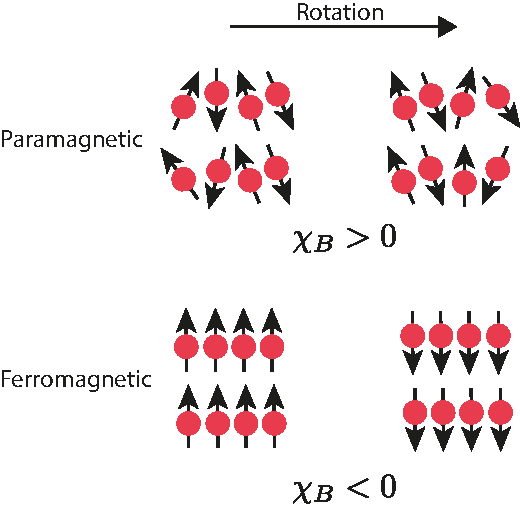
\includegraphics[width=0.36\linewidth]{./figures/ferrvspara}
    \caption{In paramagnetic materials, the spins are randomly distributed such that a rotation performed on the system will keep the spin distribution invariant. However, for ferromagnetic materials, where the spins are aligned in a single direction, the symmetry is broken, and the system has a preferred direction.}  \label{fig:paravsferro}
\end{figure}
%%%%
%%%%
\par In particle physics and quantum field theory, symmetry plays an essential role in the taxonomy and dynamics of elementary particles and their bound states, i.e. hadrons, cf.~\cite{osti_4008239,PhysRev.96.191}. There are two types of symmetries considered when studying elementary particles and their quantum fields: external and internal symmetries. The first is the symmetry of the spacetime background. Typically, this is a four-dimensional Poincar\'e symmetry. However, in some models, higher spacetime dimensions or non-flat geometries are considered. Though there is no current evidence of higher dimensions or indications of non-flat spacetime from colliders and cosmological observations~\cite{Zyla:2020zbs}. The second class of symmetries is internal symmetries stemming from the quantum nature of these particles/fields. Because their state is described by a \textbf{ray} in complex Hilbert/Fock spaces, internal symmetries are simply symmetries of rotations in these spaces that keep the action variation unchanged. Internal symmetries are usually described in terms of simple or product of simple \textbf{Lie groups}, e.g. $SU(N)$~\footnote{Gauge theories based on finite groups have been investigated in the literature, but their phenomenological significance is yet to be further investigated~\cite{Freed1993LecturesOT,dijkgraaf1990topological}}, and particles/fields will be arranged as multiplets in some representation of the groups. The rotations of the states could be parametrised by constants. In this case, the symmetry is called \textbf{global}, or fields of spacetime, where the symmetry is then called \textbf{local} or \textbf{gauged}.
%%%%
\par Gauge symmetries describe rotations in the state space that depend on spacetime, the generator of the gauge transformations could propagate between two spacetime points. This is the way particle/field interactions are described in quantum field theory. The generators of these gauge transformations are called gauge bosons, and they mediate the interactions between the particles/fields and transform under the adjoint representation of the gauge group. Hence, we observe that gauge symmetries are the basis of describing the fundamental interactions of nature, which we call \textbf{gauge theories}.
%%%%
\par An example of a gauge theory that is realised in nature is the \textbf{Standard Model}~(SM). Which is a gauge theory based on the group~$G_{\SM}:=SU(3)_C \otimes SU(2)_L \otimes U(1)_Y$. The first simple group is for the \textit{strong} interaction described by quantum chromodynamics~(QCD). The product of the two remaining groups~$SU(2)_L \otimes U(1)_Y$ forms the Weinberg-Salam \textit{electroweak}~(EW) model~\cite{salam1,salam2,PhysRevLett.19.1264}, where~$SU(2)_L$ describes the weak interaction which only couples to \emph{left handed} fermions and $U(1)_Y$ is the weak hypercharge~$Y$ gauge group, defined by the formula
\begin{equation}
    Y= 2(Q-T_3).
\end{equation}
Where $Q$ is the electric charge and $T_3$ is the third component of the weak isospin. A description of the matter content of the SM and their multiplicities with respect to~$G_{\SM}$ is shown in~\autoref{tab:thesm}
%%%%
\begin{table}[htpb!]
    \centering
    \begin{tabular}{ccc}
        \toprule
         Particle/Field& $G_\SM$ multiplicity& mass [\si{\GeV}] \\
         \midrule
         $Q = {u_L \choose d_L},{c_L \choose s_L},{t_L \choose b_L}$ & $(\irrep{3},\irrep{2},1/6)$ & $m_u=2.16\cdot10^{-3}$, $m_d=2.67\cdot10^{-3}$\\
         $U= u_R, s_R, t_R$ & $(\irrep{3},\irrep{1},2/3)$&$m_c=0.93\cdot10^{-2}$, $m_s=1.27$\\
         $D= d_R, s_R, b_R$ & $(\irrep{3},\irrep{1},-1/3)$&$m_t=172.4$, $m_b=4.18$\\
         \midrule
         $L = {\nu_{e,L} \choose e_L},{\nu_{\mu,L} \choose \mu_L},{\nu_{\tau,L} \choose \tau_L}$ & $(\irrep{1},\irrep{2},-1/2)$ & $m_e=0.511\cdot10^{-3}$, $m_\mu=1.05\cdot10^{-2}$\\
         $E= e_R, \mu_R, \tau_R$ & $(\irrep{1},\irrep{1},-1)$&$m_\tau=1.77$,$m_\nu=$??\\
         \midrule
         $g/G^A_\mu,\,\,\, A=1\dots 8$ &$(\irrep{8},\irrep{1},0)$&$ 0.0$\\
         $\gamma/A_\mu$ &$(\irrep{1},\irrep{1},0)$&$ 0.0$\\
         $W^\pm_\mu$ &$(\irrep{1},\irrep{3},0)$&$ 80.379$\\
         $Z_\mu$ &$(\irrep{1},\irrep{3},0)$&$ 91.1876$\\
         \midrule
         $h$ &$(\irrep{1},\irrep{2},1/2)$&$ 125.10$\\
        \bottomrule
    \end{tabular}   
        \caption{The SM constituents, their multiplicities with respect to the SM gauge group ~$G_{\SM}:=SU(3)_C \otimes SU(2)_L \otimes U(1)_Y$ and masses. The mass of the neutrinos $\nu$ is zero according to the SM prediction, but observations suggest that they are massive, and only the difference between the three masses is known~\cite{Capozzi:2016rtj}. The values of the masses are taken from the Particle Data Group~(PDG)~\cite{Zyla:2020zbs}, and used throughout this thesis.}\label{tab:thesm}
\end{table}

%%%%
%%%%
\par The SM has been very successful at describing particle interactions even when challenged by numerous precision tests at LEP and SLD~\cite{ALEPH:2005ab,SLD:2000jop,Group:2012gb,ALEPH:2013dgf} and later at D\O~\cite{2011baz} and the LHC~\cite{CMS:2014mgj,ATLAS:2017rzl} Nevertheless, it fails to describe the ground state if only the fermion and gauge sectors are considered. The reason for this shortcoming is that the $W^\pm$ and $Z$ bosons have a mass, this violates the EW gauge symmetry. This can be easily seen by looking at the mass term of a spin 1 field $B^A_\mu$
\begin{equation}
    \mathcal{L} = m_B B^{A,\mu}B^A_\mu,
\end{equation}
and performing an $SU(N)$ gauge transformation 
\begin{equation}
    B^A_\mu \to B^A_\mu+\partial_\mu \Lambda ^A+g \,\varepsilon^A_{BC} B^B_\mu \Lambda^C.
\end{equation}
We see that the mass term is invariant under these transformations.
Secondly, because the SM is a chiral theory, as only left-handed fermions would be doublets under~$SU(2)_L$, the Dirac mass term
\begin{equation}
    \mathcal{L}_{\mathrm{D}} = m_D \bar \psi_L \psi_R+ \hc,
\end{equation}          
cannot be a singlet under~$SU(2)_L$, hence also violating the EW symmetry. Despite quark and lepton masses being forbidden by the EW symmetry, we indeed observe that they do have a mass, and since they also carry charges this mass has to be a Dirac mass. 
\par In order for the EW model to be consistent at the ground state like it is in the interaction states. A mechanism for spontaneous symmetry breaking going from an interaction state to the vacuum ought to be introduced. 
%%%%%%
\subsection{Nambu-Goldstone theorem}
%%%%%%%
Coming back to the example of the paramagnetic-ferromagnetic materials, when heated above a certain temperature, known as the~\textbf{Curie Temperature}~$T_C$ will undergo a phase transition and become paramagnetic~(losing their permanent magnet property), in the mean-field theory approximation the magnetic susceptibility is related to the temperature of the metal via the relation
\begin{equation}
    \chi_B \sim (T-T_C)^{-\gamma},
\end{equation}  
where $\gamma$ is a critical exponent. We see that if the metal temperature $T>T_C$ the metal is in an~\textit{disordered phase} and when $T<T_C$ it is in the~\textit{ordered phase},i.e. $\chi_B$ is the \textbf{order parameter} of this system. At the Curie temperature, the system will be at the~\textit{critical point} where the susceptibility is divergent. The exponent $\gamma$ is not used to describe the system at the critical point. There is a ``pictorial'' description of the metal at the critical point which is helpful in picturing the Goldstone theorem. Starting at $T>T_C$, the metal would be in a paramagnetic phase, where the spins are randomly arranged. As the temperature becomes lower and lower, thermal fluctuations start to lessen.  One or more regions of the metal, some of the spins will start to get aligned With continued cooling, nearing $T_C$, these turned spins will affect their neighbours turning them into their directions. At the critical point $T=T_C$, the system behaves in a peculiar manner, when one would see regions of spins in ``up'' and others in ``down'' directions. The system will resemble a fractal of these regions, becoming scale-invariant. Additionally, waves of oscillating local magnetisation will propagate. These waves, or spinless quasiparticles (called \textbf{Magnons}) are Goldstone bosons emerging from spontaneous symmetry breaking. Which will manifest at $T<T_C$ as the spins will be  arranged in a certain single direction and the metal becomes ferromagnetic.
\begin{theorem}[Nambu-Goldstone]
    When a continuous symmetry has a conserved currents but broken in the ground state~(vacuum) is called to be spontaneously broken. There is a scalar boson associated with each broken generator of this spontaneously broken symmetry. The modes of these bosons are fluctuations of the order parameter.
\end{theorem}
This theorem first emerged from condensed matter physics, particularly superconductors~\cite{PhysRev.117.648,goldstone}. However, it soon got applied to relativistic quantum field theories~\cite{PhysRev.127.965}.
%%%%%%
\section{The Higgs mechanism}
%%%%%%
In order to solve the aforementioned shortcomings of the Weinberg-Salam model, Nambu-Goldstone theorem has been first proposed by P.~W.~Anderson~\cite{PhysRev.130.439}. However, the way that Anderson formulated his theory was unfamiliar to particle physicists and used a non-relativistic picture to illustrate how photons could gain mass in an electron plasma with a plasma frequency $\omega_{p}$ 
\begin{equation}
    m_\gamma^{\mathrm{plasma}} =\frac{\hbar \omega_p}{c^2}
\end{equation}
Later on, a theory that explains the mass generation of the EW gauge bosons has been published in an almost simultaneous manner by R.~Braut~ and F.~Englert~\cite{PhysRevLett.13.321}, P.~Higgs~\cite{PhysRevLett.13.508} and G.~Guralnik, C.~R.~Hagen, and T.~Kibble~\cite{PhysRevLett.13.585,Guralnik:2009jd}\footnote{All of these authors have contributed to the theory of SM spontaneous symmetry breaking~(SSB). By calling it the ``Higgs'' mechanism or boson. I, by no means, have intended to ignore the role played by the rest, rather, I wanted to stick the most widely-used terminology in the field.}.
The Higgs mechanism starts by considering the spontaneous symmetry breaking~(SSB) of the EW sector of the SM via the pattern
\begin{equation}
    SU(2)_L \otimes U(1)_Y \longrightarrow U(1)_{Q} 
\end{equation}
This is  achieved by the vacuum expectation value~(vev) of a complex scalar field $\phi\sim (\irrep{1},\irrep{2},+1/2)$, with the Lagrangian 
\begin{equation}
    \mathcal{L} = D_\mu \phi^* D^\mu \phi -V,\;\;\;\;\;\; V:= \mu^2  \phi^* \phi +\lambda (\phi^* \phi)^2,
    \label{higgspot}
\end{equation}
 were $\phi$ is given explicitly by 
 \begin{equation}
  \phi = \begin{pmatrix}
      \phi^1 + i \phi^2\\  \frac{1}{\sqrt{2}}(h+v)-i \phi^3
  \end{pmatrix}
\end{equation}
The covariant derivative 
\begin{equation}
    D_\mu= \partial_\mu -ig_2\frac{\sigma_a}{2}W^a_\mu-ig_1\frac{1}{2} B_\mu,   
\end{equation}
dictates the coupling between the Higgs field and the EW gauge bosons and~$g_3$, $g_2$ and $g_1$ are, respectively, the coupling constants of 
${ SU(3)_C}$,  ${ SU(2)_L}$ and  ${ U(1)_Y}$.  
 The minimum of the scalar potential is then obtained by
 \begin{equation}
\frac{\partial V}{\partial \phi} \mid_{\phi\to v} = 0,
\end{equation}
which for a tachyonic mass~$\mu^2 < 0$ will have a real non-vanishing values~$v$ corresponding to the vev of this field~$\langle \phi \rangle ={0\choose \frac{v}{\sqrt{2}}}$.\\
According to Nambu-Goldstone theorem, the three broken generators of~$SU(2)_L \otimes U(1)_Y$ will become massive, and they are the $W^\pm$ and $Z$ bosons, while the photon will remain massless. We will have three massless Goldstone bosons $ G^\pm=\frac{1}{2} (\phi^1\pm i\phi^2) $ and $G^0=\phi^3$ that are ``eaten'' by the aforementioned massive photons. Where they become the longitudinal polarisations of $W^\pm$ and $Z$ boson. In order to see this more concretely, we start by looking at the terms of the EW Lagrangian where the field $\phi$ couples to the gauge bosons, in the unbroken phase
\begin{equation}
   D_\mu \phi^* D^\mu \phi = \frac{1}{2} |\partial_\mu \phi|^2 + \frac{1}{8}g_2^2|\phi|^2|W_\mu^1+iW_\mu^2|^2
   + \frac{1}{8}|\phi|^2 |g_2 W_\mu^3- g_1 B_\mu|^2
   \label{ewhiggs_ub}
\end{equation}
After SSB, we write the gauge bosons in the mass basis~
\begin{align}
W_\mu^\pm &= \frac{1}{\sqrt{2}} (W^1_\mu\pm iW^2_\mu), \nonumber \\
Z_\mu &= \frac{1}{\sqrt{g_1^2+g_2^2}} \left(g_2 W^3_\mu-g_1B_\mu\right), \\
A_\mu &= \frac{1}{\sqrt{g_1^2+g_2^2}} \left(g_2 W^3_\mu+g_1B_\mu\right). \nonumber
 \end{align}
 From this, the electric change is identified as the coupling constant to the photon~$A_\mu$ 
 \begin{equation}
     e=\frac{g_1}{\sqrt{g_1^2+g_2^2}}.
 \end{equation}
 It is useful to define~\textbf{Weinberg angle}~$\theta_W$, an important EW parameter relating the electric charge to the weak coupling~$g_2$ 
 \begin{equation}
     \sin \theta_W = \frac{e}{g_2} \approx 0.231214,
 \end{equation}
 typically the $\sin$ and $\cos$ of the Weinberg angle are denoted by $s_W$ and $c_W$, respectively. \\ We use the unitary gauge, to absorb the Goldstone bosons into the $W^\pm$ and $Z$ longitudinal polarisations. In this gauge the Higgs doublet can be written as
\begin{equation}
    \phi \to \begin{pmatrix}
       0\\  \frac{1}{\sqrt{2}}(h+v).
    \end{pmatrix}, \,\,\,\,\,\,\,\, v= 246\, \mathrm{GeV}.
    \label{unitaryhiggs}
  \end{equation}
With these substitutions, one can read off the masses of the gauge bosons their bilinear terms in~\eqref{ewhiggs_ub}
\begin{align}
    m_W =& \frac{vg_2}{2} & m_Z&=\frac{v}{2}\sqrt{g_1^2+g_2^2} & m_A &= 0.
\end{align}
Since $\phi$ is a complex doublet. We have seen that it has four components,  and three of them correspond to the Goldstone bosons, thus one remains physical~$h$ which is what we now identify with the ``Higgs boson'' discovered in the Summer of 2012~\cite{CMS:2012qbp,ATLAS:2012yve}. The couplings between  the Higgs and the electroweak bosons is related to their mass via the vev 
\begin{align}
    g_{hVV} =& \frac{2 m_V^2}{v}, & g_{hhVV}=& \frac{2 m_V^2}{v^2}.
\end{align}
By substituting~\eqref{unitaryhiggs}, into the Higgs potential~\eqref{higgspot} one can write the mass of the physical Higgs boson in terms of the vev
\begin{align}
  m_h =\sqrt{2 \lambda} v .
\end{align}
The physical Higgs mass is related to the $\mu$ parameter via the relation
\begin{align}
	m_h ^2 =-2 \mu^2,
\end{align}
One can see that the mass term after SSB changes its sign, characterising the order-parameter for this system,  analogous to the magnetic susceptibility for the magnetisation of materials example. 
One could also identify the self-couplings of~$h$, the trilinear and quartic couplings 
\begin{align}
    g_{hhh}&=3\lambda v =3\frac{m_h^2}{v}, & g_{hhhh}&= 3 \lambda = 3\frac{m_h^2}{v^2}.
\end{align}
%%%
\section{Yukawa interaction}
It is possible to also use the Higgs vev to give fermions their masses by introducing a Yukawa-interaction terms, first introduced by S. Weinberg~\cite{PhysRevLett.19.1264}
\begin{equation}
    \mathcal{L}_{\mathrm{Yuk}}= -y_{e} \, \bar{L} \, \phi \, E 
- y_{d} \, \bar{Q} \, \phi \, D
- y_u \, \bar{Q} \, \tilde{\phi} \, U   \ + \hc,
\label{lag-yuk}
\end{equation}
with $ \tilde{\phi}= i\sigma_2 \phi$ and $ y_e, y_d, y_u$ are $3\times 3$ matrices. These matrices are free parameters in the SM. As the Higgs boson acquires a the vev, the fermions will acquire a mass $m_f= vy^\prime_f$ and the Higgs boson coupling to the fermions is given by
\begin{equation}
	g_{h\bar{f}f} = \frac{m_f}{v},
\end{equation}
 and the Yukawa matrices will be fixed in the mass basis ~$y^\prime_f$ by measurements of the fermion masses.\\  Leptonic Yukawa matrix is diagonal, with a degeneracy between the flavour and masses basis, this manifests as lepton family number conservation~(the lepton family operator commutes with the Hamiltonian.). However, for the quarks, the situation is more complicated. One can rotate these matrices to the mass basis via a bi-unitary transformation via the unitary matrices~$ \mathcal{V}_Q, \mathcal{U}_Q$ for $ q= u,d$
\begin{equation}
    y_{q} \longrightarrow y^\prime_f= \mathcal{V}^\dagger_{q} \,y_q\, \mathcal{U}_{q} = \text{diag}\left(m_{q_1}, m_{q_2},m_{q_3}\right).
\end{equation}
However, the is no degeneracy here as the Hamiltonian does not commute with the quark flavour operator. This is because the transformation matrices for the up and down-type quarks are not the same.  The charged EW quark currents contains flavour mixing described by the Kabibbo-Kobayashi-Maskawa~(CKM) matrix~\cite{PhysRevLett.10.531,10.1143/PTP.49.652}. More details on the flavour sector of the SM is discussed in~\la{Update the section}\\
\autoref{fig:SMcouplings} shows all the SM couplings' strengths, with the thickness of the chord is proportional to the strength of the coupling, on can see the Higgs couplings in orange. 
%%%%
\begin{figure}[htpb!]
    \centering
    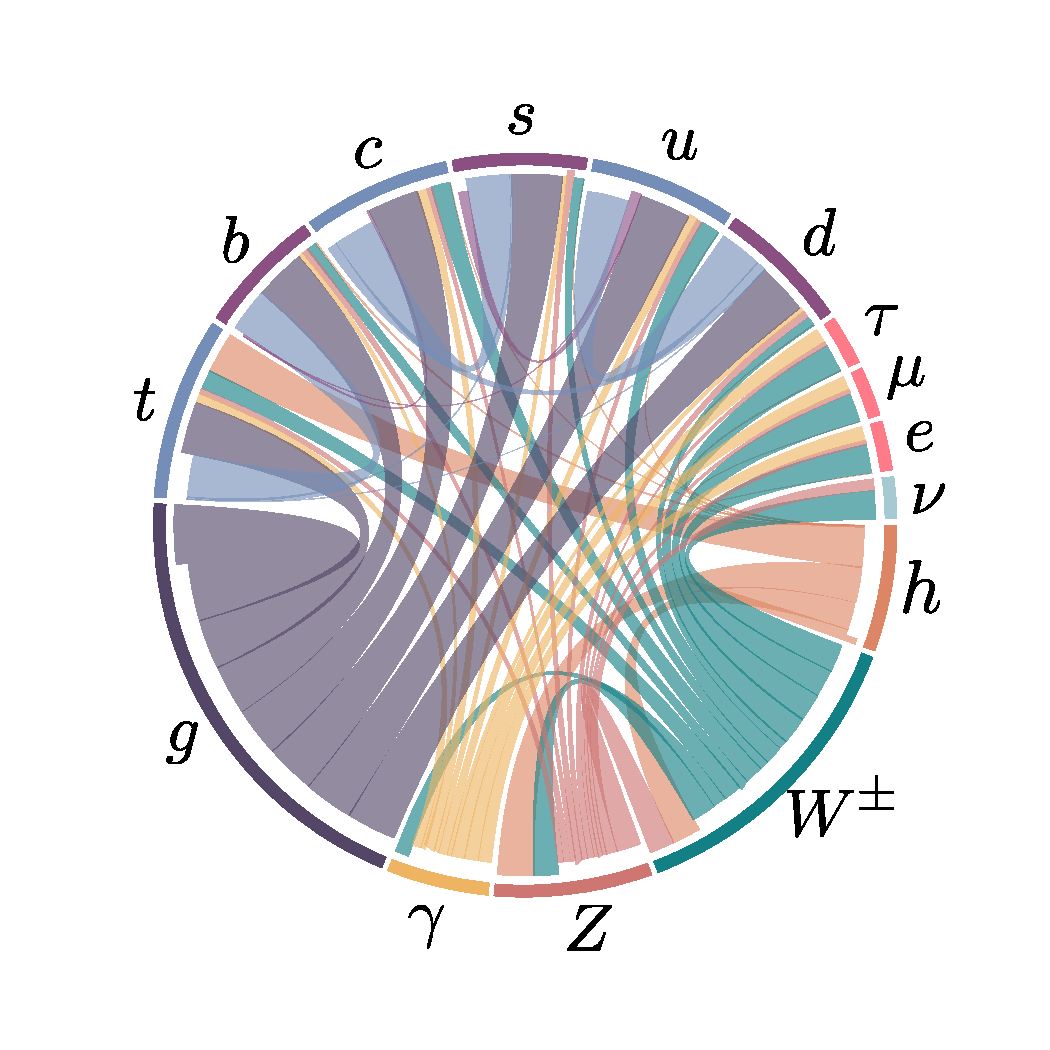
\includegraphics[width=\linewidth]{./figures/SM}
    \caption{A chord diagram showing the SM couplings, with the coupling strength illustrated by the chord thickness. Higgs couplings are coloured in orange.}  \label{fig:SMcouplings}
\end{figure}
%%%%
%%%%
\section{The Higgs and EW precision observables}
\par Higgs physics is intertwined with the EW sector for example, the Higgs vev is determined from Fermi's constant~$v =(\sqrt{2}G_F)^{-1/2}$, and is fixed by muon lifetime measurements, and comparing it with the theoretical predictions~\cite{PhysRev.101.866,PhysRev.113.1652,Mohammad:1976qd,PhysRevLett.82.488} 
\begin{equation}
    \tau_\mu^{-1} = \frac{G_F^2 m_\mu^5}{192\pi^3}\left(1-\frac{8 m_e^2}{m_\mu}\right) \left[1-1.810\frac{\alpha}{\pi}+(6.701\pm0.002)\left(\frac{\alpha}{\pi}\right)^2\right],
\end{equation}
which leads to the numerical value of $G_F$~\cite{Zyla:2020zbs}
\begin{equation}
    G_F=1.1663787(6) \cdot 10^{-5} \si{\per\GeV\squared},
\end{equation}
given the value of the fine structure constant~$\alpha^{-1} =137.03599976 (50)$. 
\par Another important EW precision observable~(EWPO) is the ratio between the $W$ and $Z$ masses
\begin{equation}
    \rho = \frac{m_W^2}{c_W^2m_Z^2}.
\end{equation}
At leading order, this parameter is equal to unity in the SM. The $\rho$ parameter depends on the representation of the scalar sector of the EW model having $\phi_i$ scalars with $T_i$ weak isospin and $T_{3,i}$ being its third component, and a vev $v_i$, via the relation~\cite{ROSS1975135,Djouadi:2005gi}
\begin{equation}
    \rho =\frac{\sum_i [T_{i}(T_{i}+1)-T_{3,i}^2]v_i^2}{2\sum_i T_{3,i}^2v_i^2}.
    \label{rhohiggs}
\end{equation}
From~\eqref{rhohiggs} one can see that a real triplet scalar, for instance, would not fit the experimental EW measurement of $\rho$. Hence, a complex doublet is the simplest scalar possible for the EW symmetry breaking, and the Higgs boson was expected to be seen almost four decades before its discovery. However, radiative corrections to the EW gauge bosons mass from vacuum polarisation diagrams could potentially cause $\rho$ to deviate significantly from unity.  This is not the case, as the experimentally measured value of~$\rho$~\cite{Zyla:2020zbs}
\begin{equation}
    \rho_{\text{exp}} = 1.00038 \pm 0.00020
    \label{eq:rhoexp}
\end{equation}
Additionally, it is possible to think of an extended Higgs sector, where there are multiple scalars with different $SU(2)_L$ multiplicities. Or, a composite Higgs sector, where the Higgs boson is a pseudo Nambu-Goldstone boson, cf.~\cite{Dugan1985AnatomyOA,Hill:2002ap}. How can such models be built assuring the $\rho$ parameter is protected from change ? The answer to this question lies in a symmetry of the Higgs Lagrangian known as custodial symmetry. 
\subsection{Custodial symmetry}
After SSB, a residual global symmetry known as the custodial symmetry protects the $\rho$ parameter from obtaining large radiative corrections at higher orders in perturbation theory.  This symmetry must be kept in extended or composite Higgs models. This symmetry can be seen by rewriting the Higgs potential as
\begin{equation}
	V = \frac{\lambda}{4} \left(å \phi_1^2+\phi^2_2+\phi_3^2+\phi^2_4 -2 \mu^2\right)^2.
\end{equation}
This potential is invariant under $SO(4)\simeq SU(2)_L \otimes SU(2)_R$ rotations. However, when the Higgs field squires a non-vanishing vev,  $ \phi_4 \to h+v$, the potential becomes
 \begin{equation}
 	V = \frac{\lambda}{4} \left( \phi_1^2+\phi^2_2+\phi_3^2+ h^2+2vh+v^2 -2 \mu^2\right)^2,
 \end{equation}
which is only invariant under  $SO(3)\simeq SU(2)_V$ transformations, the diagonal part of the original group. This global SSB pattern comes alongside the EW SSB of the gauge group $SU(2)_L \otimes U(1)_Y$ as global $SU(2)_L$ is itself the gauged $SU(2)_L$  group. Additionally the $T^3$ component of the ~$SU(2)_R$ global group is the gauged $U(1)_Y$ and the~$T^3$ component of the custodial group~$SU(2)_V$ is gauged as well and identified to be the electric charge operator, i.e. the generator of $U(1)_Q$. 
\begin{equation}
	\underbrace{SU(2)_R}_{{\color{myblue} \supset\, U(1)_Y}} \otimes \overbrace{SU(2)_L}^{{\color{myblue} \text{gauged}}} \longrightarrow \underbrace{SU(2)_V}_{{\color{myblue} \supset\, U(1)_Q}} .
\end{equation}
This pattern indicates that the symmetry is already broken by the gauging of the diagonal part of $SU(2)_R$ ~(the hypercharge). The custodial symmetry is only \emph{approximate} in the limit of $ g_1 \to 0$, and $\rho=1$ is a consequence of $g_1\neq 0$ . The symmetry breaking pattern $\irrep{2} \otimes \irrep{2} = \irrep{3} \oplus \irrep{1}$ also allows us to identify the Goldstone bosons as the custodial triplet and the physical Higgs~$h$ as the custodial singlet, explaining the electric charge pattern they have.   \\
 We could use the isomorphism between the special orthogonal and special unitary groups to parametrise the Higgs doublet as an 
$SU(2)_L \otimes SU(2)_R$ bidoublet 
\begin{equation}
	\mathcal{H} =(\tilde{\phi} \,\,\, \phi) = \frac{1}{\sqrt{2}}\begin{pmatrix}
		\phi_4-i\phi_3 & \phi_1+i\phi_2 \\
		 \phi_1-i\phi_2 & \phi_4+i\phi_3
	\end{pmatrix},
\end{equation}
with the bi-unitary transformations
\begin{equation}
	\mathcal{H} \longrightarrow \mathcal{U}_L \mathcal{H} \mathcal{U}^\dagger_R
\end{equation}
which leaves any traces of the form $\mathrm{Tr}(\mathcal{H}^\dagger\mathcal{H})$, invariant. The Higgs potential could be rewritten in terms of the bidoublet 
\begin{equation}
	V = -\frac{\mu^2}{2} \mathrm{Tr}(\mathcal{H}^\dagger\mathcal{H} + \frac{\lambda}{4}\left(  \mathrm{Tr}(\mathcal{H}^\dagger\mathcal{H} \right) ^2
\end{equation}
The vev is hence written in this representation as 
\begin{equation}
\langle \mathcal{H} \rangle  = \frac{v}{\sqrt{2}}\, \mathbb{1}_{2\times 2}.
\end{equation}
We can also look at the Yukawa sector, and observe that in the case where $ y_u =y_d =y $, we can also write the left-handed and right-handed quarks  as $SU(2)_L \otimes SU(2)_R$  bidoublets and $SU(2)_R$ doublets, respectively. Hence, the quark part of the Yukawa Lagrangian in~\eqref{lag-yuk} becomes
\begin{equation}
	\mathcal{L}_{yuk} \supset \frac{y}{\sqrt{2}}  (\bar u_L\,\,\, \bar d_L)  \begin{pmatrix}
		\phi_4-i\phi_3 & \phi_1+i\phi_2 \\
		\phi_1-i\phi_2 & \phi_4+i\phi_3  
	\end{pmatrix}  \begin{pmatrix}  u_R \\ d_R	\end{pmatrix} ,
\end{equation}
which is invariant under custodial transformations, but when~$ y_u \neq y_d$, this Lagrangian term breaks custodial symmetry. Thus, the differences between the up-type and down-type quark masses $m_u-m_d$ are considered \textbf{spurions} of the  custodial symmetry and one expects to see radiative corrections to $\rho$ being proportional to these spurions.
\par In order to see this more concretely, we start by examining the radiative corrections that could contribute to the deviation of $\rho$ from unity, i.e. $\Delta \rho$ these corrections are known as the \textbf{oblique correction}. These oblique corrections come from electroweak vacuum polarisations~$\Pi_{VV}(p^2)$, as shown in ~\autoref{fig:oblique}, for more details on these corrections and their calculation see Refs..~\cite{schwartz2014quantum,peskin1995introduction} \\
%%%%
\begin{figure}[htpb!]
	\centering
	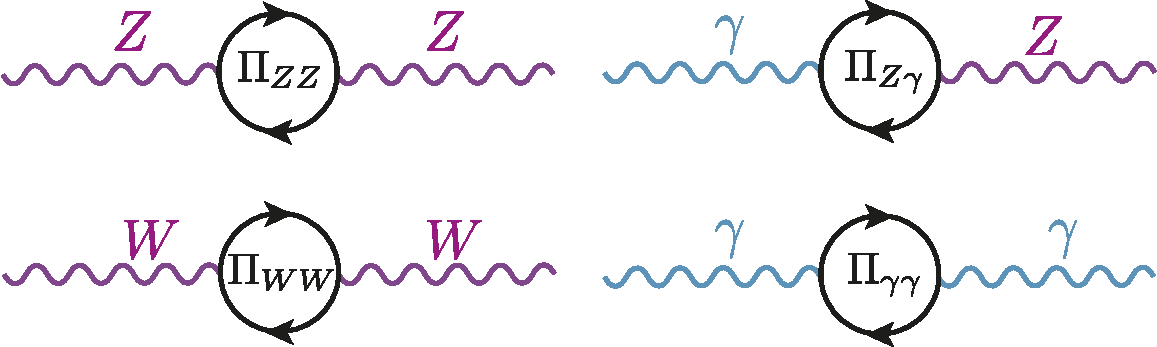
\includegraphics[width=0.75\linewidth]{./figures/oblique_corrections}
	\caption{The oblique corrections, are radiative correction with electroweak gauge bosons propagators. Namely vacuum polarisations of the $Z$, $W^\pm$ and $\gamma$ bosons. }  \label{fig:oblique}
\end{figure}
%%%%
%%%%
The 1-loop correction to the $\rho$ parameter is given in terms of the ~$\Pi_{VV}$  by
\begin{equation}
\Delta \rho = \frac{\Pi_{WW}(0)}{m_W^2}- \frac{\Pi_{ZZ}(0)}{m_Z^2}
\end{equation}
Where the dominant contributions are given by~\cite{EINHORN1981146}
\begin{align}
\Delta \rho & = \frac{3 G_F}{8\sqrt{2}\pi^2}\,\left((m_t^2+m_b^2)-\frac{2m_t^2m_b^2}{m_t^2-m_b^2}\ln \frac{m_t^2}{m_b^2} \right)+\dots.
\label{eq:deltarho}
\end{align}
Since $m_b\ll m_t$, the correction is non-vanishing, and~\eqref{eq:deltarho} shows clearly how the radiative corrections are proportional to the spurions of the custodial symmetry. However, this radiative correction is absorbed into the SM definition of $\rho$, i.e. the $\MSbar$ definition of the $\rho$-parameter~$\rho^{\MSbar}$.
\par One can study  new physics~(NP) effects that violates custodial symmetry, by looking at deviations from $\rho=1$ from it. Given the experimentally measured value of~$\rho$~\eqref{eq:rhoexp} many NP models violating custodial symmetry can already be excluded. Nevertheless, $\rho$ alone does not capture the full story of~EWPO's. For instance, adding a new quark doublet would not necessarily violate the custodial symmetry though it still can be excluded by EWPO. It is hence useful to introduce new parameters known as \textbf{Peskin-Takeuchi parameters}~\cite{PhysRevLett.65.964,Peskin91estimationof,peskin1995introduction}
\begin{align}
	S &:=\frac{4 c_W^2 s_W^2}{\alpha} \left[ \frac{\Pi_{ZZ}^{\NP} (m_Z^2)- \Pi_{ZZ}^{\NP} (0)}{m_Z^2}  - \frac{c_W^2-s_W^2}{c_Ws_W}\,\frac{\Pi_{Z\gamma}^\NP(m_Z^2)}{m_Z^2}-\frac{\Pi_{\gamma\gamma}^\NP(m_Z^2)}{m_Z^2}\right],  \nonumber \\
	T &:=\frac{\rho^{\MSbar}-1}{\alpha}  = \frac{1}{\alpha} \left[ \frac{\Pi^\NP_{WW}(0)}{m_W^2}- \frac{\Pi^\NP_{ZZ}(0)}{m_Z^2} \right] , \\
	U&:= \frac{4 s_W^2}{\alpha} \left[ \frac{\Pi_{WW}^{\NP} (m_W^2)- \Pi_{WW}^{\NP} (0)}{m_W^2}   - \frac{c_W}{s_W}\,\frac{\Pi_{Z\gamma}^\NP(m_Z^2)}{m_Z^2}-\frac{\Pi_{\gamma\gamma}^\NP(m_Z^2)}{m_Z^2}\right] -S .\nonumber 
\end{align}
The NP contributions to the EW vacuum polarisations $\Pi_{VV}^{\NP}(p^2)$) could either come from loop or tree-level effects. Typically both $T$ and $U$ are related to custodial symmetry violation. However, $U$ has an extra suppression factor of $m_\NP^2/m_Z^2$ compared to $T$ and $S$. The most recent fit result for these parameters is~\cite{Zyla:2020zbs}
\begin{align}
	S &=-0.01\pm0.10,  \nonumber \\
	T &= 0.03\pm0.13, \\
	U&:= 0.02\pm0.11.\nonumber 
\end{align}
But since $T$ and $S$ tend to give stronger constraint on NP, due to the suppression factor of $U$. One can preform a two-parameter fit of $S$ and $T$ setting $U=0$, thas shown in~\autoref{fig:stubound}, with the numerical values~\cite{Zyla:2020zbs}, \\
 \begin{align}
 	S &=0.00\pm0.07,  \nonumber \\
 	T &= 0.05\pm0.06.
 \end{align}
%%%%
\begin{figure}[t]
	\centering
	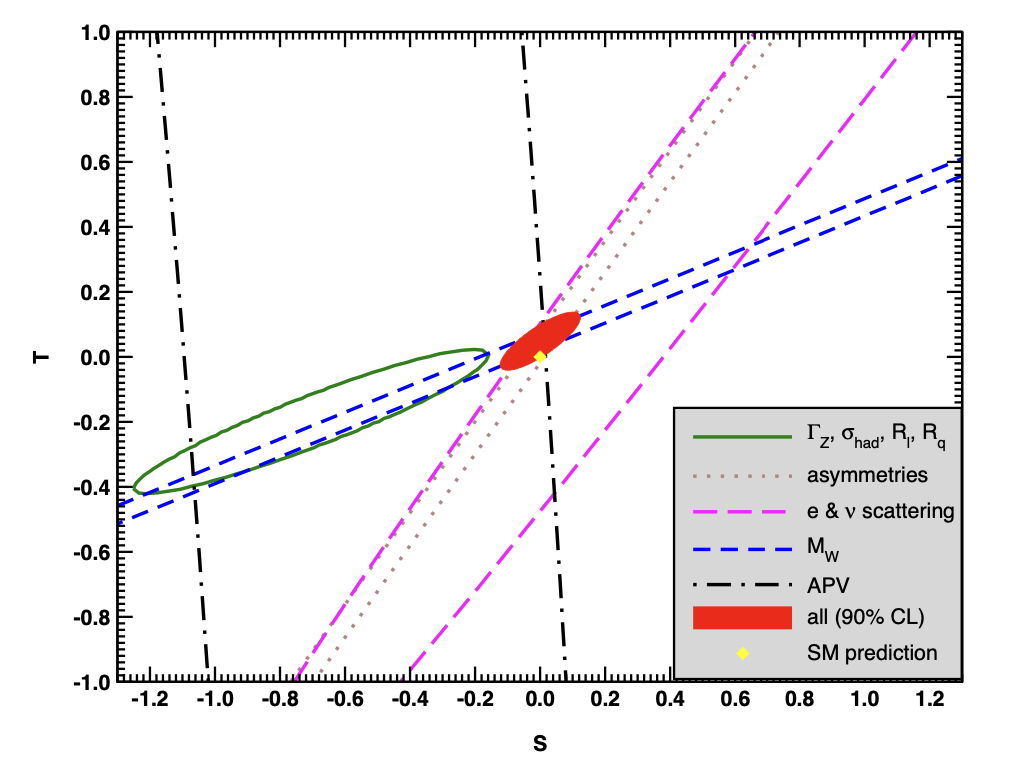
\includegraphics[width=0.65\linewidth]{./figures/stu-pdg}
	\caption{ Fit results from various EWPO's for $T$ and $S$ setting $U=$. The contours show $1\,\sigma$ contours~(39.35\% for closed contours and 68\% for the rest). This plot is obtained from the PDG~\cite{Zyla:2020zbs}  }  \label{fig:stubound}
\end{figure}
%%%%
%%%%
The Peskin-Takeuchi parameters are important in constraining effective operators in the Higgs sector , namely
 \begin{align}
 \hat{O}_S &= \phi^\dagger \sigma_i \phi W^i_{\mu \nu} B^{\mu \nu}, \nonumber \\
\hat{O}_T &= |\phi^\dagger D_\mu \phi|^2.
\end{align}
For example, $\hat{O}_S$ appears in Technicolour models causing large deviations of $S$ compared to its measured value~\cite{GOLDEN19913,HOLDOM199088,ALTARELLI19923,PhysRevLett.65.964}. Moreover, The constraints on $T$ parameter is important for top mass generation ans well as modifications to~$Z  b \bar{b}$ coupling in such models~\cite{PhysRevLett.69.575,Simmons:1995df}. We will revisit the $\hat{O}_T$ when we discuss the Higgs and effective field theories in section \la{update here}.
       
        %%!TEX encoding = UTF-8 Unicode
% !TeX spellcheck = en_GB
%%%%%%%%%%%%%%%%%%%%%%%%%%%%%%%%%%%%%%
\chapter{Experimental measurements of the Higgs boson }\label{chap:HiggsConstr}
%%%%%%%%%%%%%%%%%%%%%%%%%%%%%%%%%%%%%%
%In this chapter, I will discuss some of the bounds on the Higgs sector . Starting from an overview of the theoretical constraints on the Higgs potential, like the quantum triviality and unitarity. Then, the state-of-the-art experimental results on Higgs properties and couplings measurements will be discussed. However, despite many of the Higgs boson properties have been measured with good accuracy, there are still difficult observables in the Higgs sector and some open problems. These will be addressed at the end of this chapter.   
%%
The observation of the Higgs boson, then the extensive measurement of its properties and couplings has been on the top of the LHC programme priorities~\cite{ellis2000physics}. In the time this thesis was in the writing, the particle physics community will be celebrating a decade since the Higgs boson's discovery. Looking back 10 years ago, when I have witnessed the discovery of the Higgs boson via news press-conference in summer of 2012, and decided to be a part of this enormous step that humanity has taken, 
I feel astonished by the progress made in understanding this newly discovered particle!  \\ In this chapter, I will start by an overview of the extraordinary LHC and its experiments~in~\autoref{sec:theLHC}. Then, I will review the state-of-the-art status of experimental measurements of the Higgs properties in~\autoref{sec:Higgsprop}, cross-sections  and couplings in ~\autoref{sec:Higgscoupl}, and at the end I will discuss the challenges and outlook for the future runs of the LHC~\autoref{sec:Higgscouplchallenge}, of which the of the rest of this thesis is going to be aim address a small part of them.
\section{Overview of the Large Hadron Collider \label{sec:theLHC}}
\par The Large Hadron Collider~(LHC) is the largest particle accelerator in the CERN accelerators complex, with a circumference of about 26 \si{\kilo\metre},with over 9590 superconducting magnets cooled to 1.9 \si{\kelvin}. It was built as an upgrade to the  Large electron positron collider~(LEP) which ended its operation in the year 2000. The LHC contains four main experiments situated at the four beam collision points and detectors, and these experiments are: ATLAS, CMS, LHCb and ALICE, there also smaller experiments such as LHCf, MilliQan,TOTEM and others. For more details about the LHC cf.~\cite{cernfacts,welt-machine} or see the LHC technical design report~\cite{Bruning:2004ej} for more technical details.\\   The LHC started operation in September of 2008, with low energy proton beams, then gradually increased to an energy of 3.5 \TeV\ per proton to reach a centre of mass energy~$\sqrt{s}$ of 7 \TeV, and data-taking period started from 2011 . By 2012, its energy has increased to $\sqrt{s}= 8\ \TeV$ and operated at this energy for about year and half, then stopping in mid 2013 concluding what is known as \textbf{Run-I}. In 2015, the \textbf{Run-II} started with almost double the energy $\sqrt{s}= 13\ \TeV$, and lasted for ca. 3 years. As this thesis being written, preparations are being made to get \textbf{Run-III} started until 2024. During these runs, heavier nuclei such as $\prescript{207}{}{\mathbf{Pb}}$ and $\prescript{131}{}{\mathbf{Xe}}$ have been collided either with protons or with themselves~\cite{lhckomission}.  \\  From, 2025 and beyond, the \textbf{High-Luminosity} LHC~(HL-LHC) era will commence, see~\autoref{fig:lhcplan}.   Where the LHC will be shutdown for extensive upgrades ~\cite{Apollinari:2015bam} to potentially increase its energy to  $\sqrt{s}= 14\ \TeV$ and higher collision rates hence the term \emph{high luminosity}. Which leads us to an important notion in particle physics phenomenology ~\emph{integrated luminosity}.\\
\par The performance of colliders depends on many factors, but for phenomenological studies, like this thesis, one mainly considers the centre of mass energy $\sqrt{s}$ and the integrated luminosity~$\mathscr{L}$.
This is mainly due to the fact that particle colliders experiments are basically ``counting experiments'', and all of the bounds on physical observables or model parameters are obtained from the number of signal versus background events, and the number of expected events~$N_{expec}$ for a given resonance $R$ and a subsequent decay final state $X$ at any collider experiments is given by
\begin{equation}
	N_{expec} = \sigma(pp\to R) \, \mathcal B(R \to X)\,\mathscr{L}  \, \epsilon_{\mathrm{SEL}}.
\end{equation}
Here $ \epsilon_{\mathrm{SEL}}$ is the selection efficiency, which depends on many factors like the detector geometry and particle identification performance etc. , as well as the signal one searches for, it can be improved by better detected or selection cuts. The production cross-section increases typically with quadratically with $\sqrt {s}$, hence comes the need for higher energies but this can only achieved by building new colliders from scratch. The integrated luminosity can be increased much more easily, by longer running time of the same collider as it is the time integral of the collider's luminosity $L(t)$ over its operation time $T$
\begin{equation}
\mathscr{L} = \int^{T} L(t) .
\end{equation}
Therefore, we see that the integrated luminosity for the LHC experiments will increase over time, when more collisions taking place, as seen in figure~\autoref{fig:lumi} showing the integrated luminosity for ATLAS and CMS experiments. 
\begin{figure}[t!]
	\begin{center}
		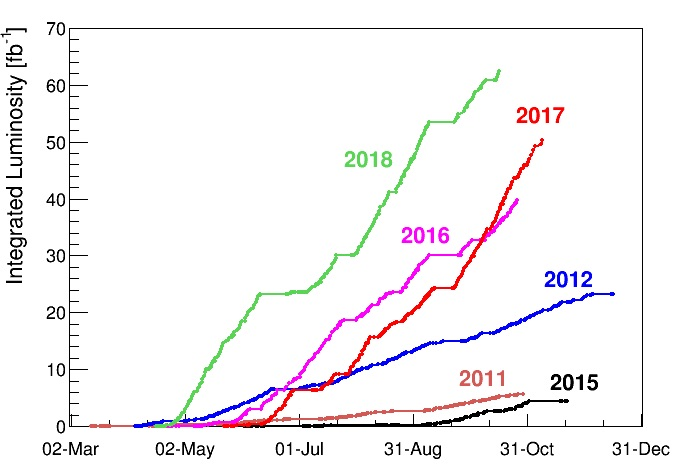
\includegraphics[width=8cm]{figures/lhc_lumi}
		\caption{The integrated luminosity of the CMS and ATLAS experiments combined over the period from 2011-2018, source~\cite{lhcpreformance}.  \label{fig:lumi} }
	\end{center}
\end{figure}
As thee protons travel in the LHC in \textbf{bunches}, and as these bunches cross, protons collide at a certain frequency $f$,  when two bunches with $N_1$ and $N_2$ protons per bunch, respectively. Each bunch will have an effective cross-section~$4 \pi \sigma_i$ corresponding to their physical sizes $\sigma \sim \SI{16}{\micro \meter}$, the luminosity is therefore given -approximately- by 
\begin{equation}
	L = \frac{f N_1 N_2}{4 \pi  \sigma_1 \sigma_2},
\end{equation}
which is for the LHC averages to about $ 10^{34}$ collisions \si{\per \centi\metre\squared \per \second}~\cite{closer,lhcpreformance}.  \\ The total physics-viable $pp$-collisions  integrated luminosity for Run-I was \SI{4.57}{\per \femtobarn} for \SI{7}{\tera\electronvolt} and \SI{20.3}{\per \femtobarn} for \SI{8}{\tera\electronvolt} (ATLAS~\cite{atlaslumi1}) and  \SI{5.55}{\per \femtobarn} at \SI{7}{\tera\electronvolt} and \SI{21.8}{\per \femtobarn} at \SI{8}{\tera\electronvolt} (CMS ~\cite{cmslumi}). As for Run-II the integrated luminosity is \SI{139}{\per \femtobarn} at \SI{13}{\tera\electronvolt } (ATLAS~\cite{atlaslumi2})  and \SI{137}{\per \femtobarn} at \SI{13}{\tera\electronvolt } (CMS ~\cite{cmslumi}). The expected integrated luminosity by the end of Run-III is  \SI{300}{\per \femtobarn}~\cite{Fartoukh:2790409} and \SI{3000}{\per \femtobarn} by the end of the HL-LHC at energy of \SI{14}{\tera\electronvolt }~\cite{Apollinari:2015bam}. 
\begin{sidewaysfigure}[ht]
	\centering
		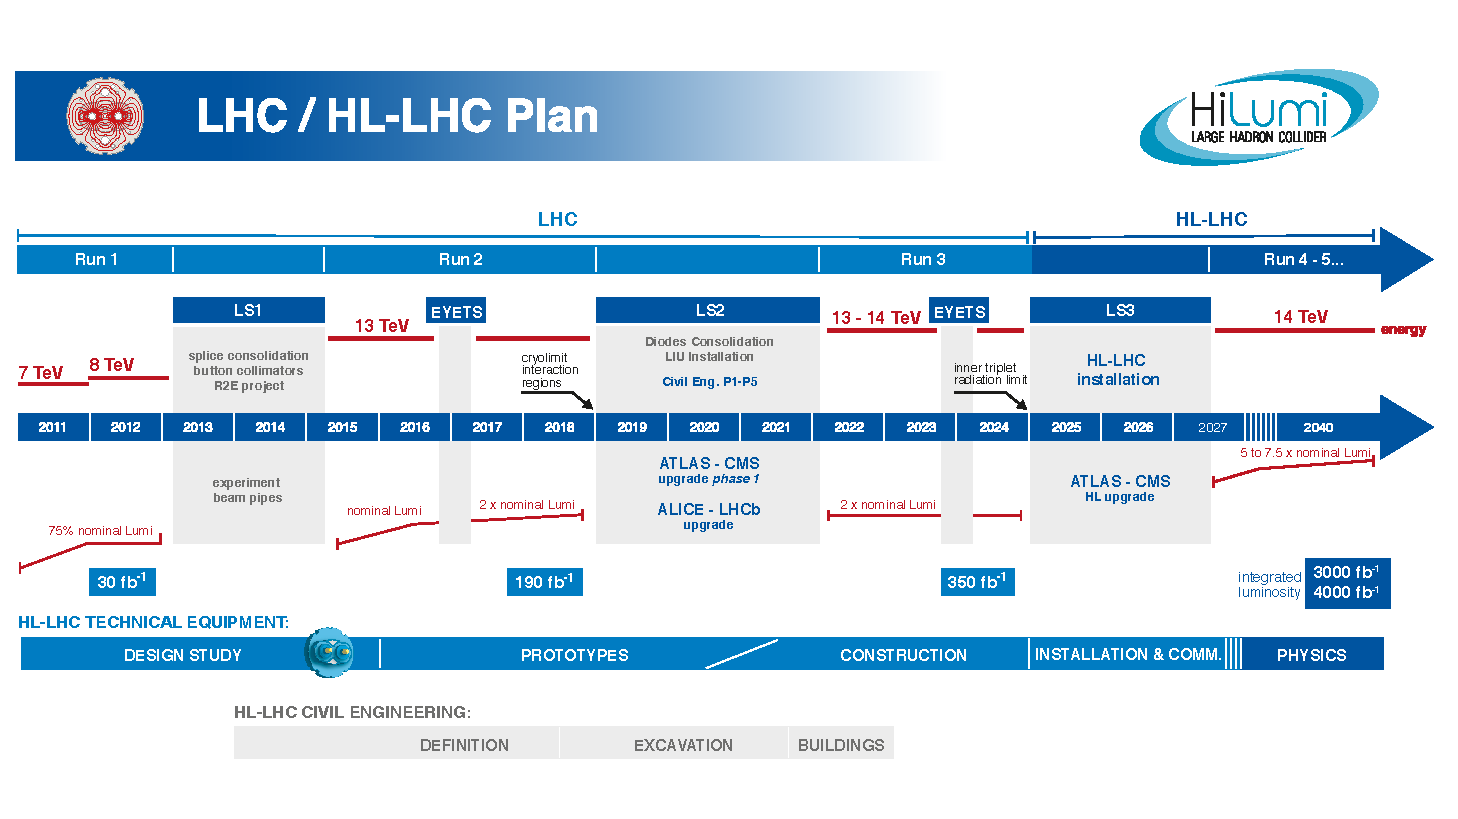
\includegraphics[width=\textwidth]{figures/HL-LHC-plan-2021-1}
	\caption{ A timeline of the LHC operation showing Run-I, Run-II and future planned runs of the LHC, including the HL-LHC, source~~\cite{lhckomission}. 
	}
\label{fig:lhcplan}
\end{sidewaysfigure}
\FloatBarrier
\section{Higgs properties \label{sec:Higgsprop} }
\subsection{Higgs boson mass measurements}
In order to measure the mass of thee Higgs boson with high precision, one need to consider final states that can be reconstructed with high momentum and mass resolution, this is typically achieved when no hadronic constituents in the decays involved, such as  $ h \to \gamma \gamma$ and $ h \to Z Z^*\to 4 \ell$. Reconstructing the invariant mass distributions $m_{\gamma \gamma}$ and $m_{4\ell}$ one observes that the Higgs peak is narrow over a relatively smooth background, see~\autoref{fig:higgs_mass}, which is ideal for the measurement of the Higgs mass. It should be noted that the width of the resonance is due to the detector resolution and does not correspond to the actual Higgs width.\\
\begin{figure}[t!]
	\begin{center}
		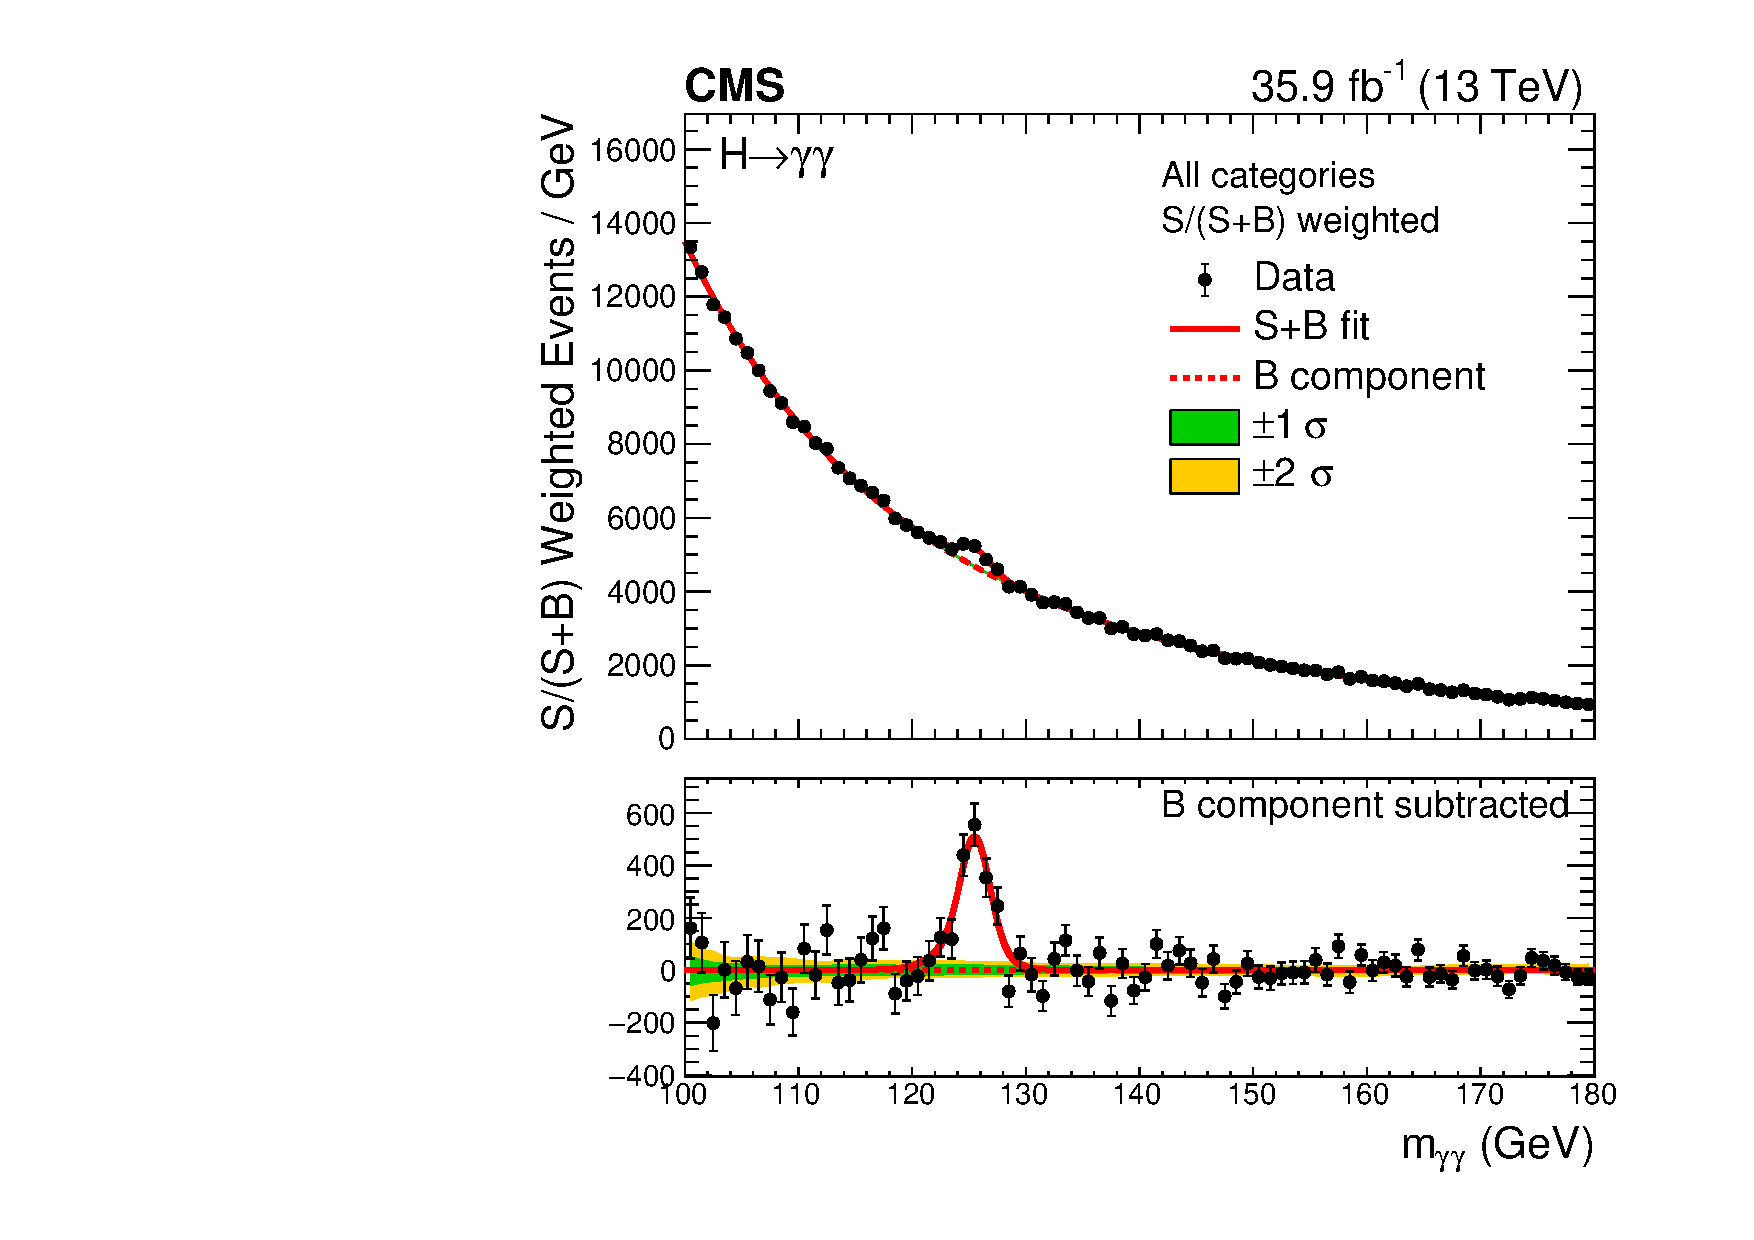
\includegraphics[width=0.45\textwidth]{figures/Higgs_results/CMS-HIG-19-004_Figure_005-b}
		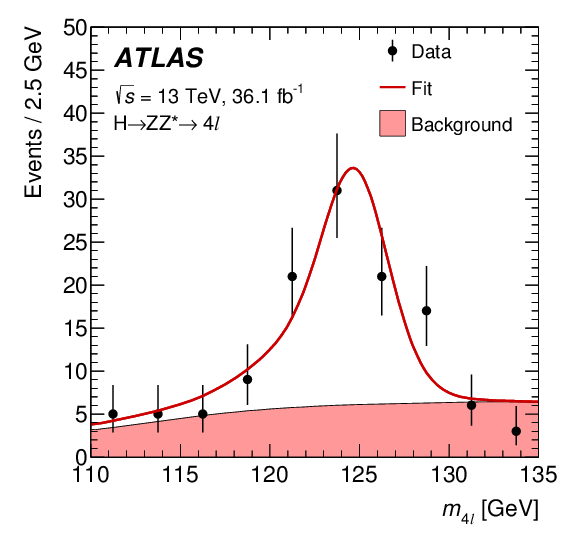
\includegraphics[width=0.45\textwidth]{figures/Higgs_results/dataAll_H4l_m4l_pdf_constrained} 
		\caption{The invariant mass distributions of diphoton~$m_{\gamma \gamma}$ (CMS~\cite{CMS:2020xrn}) and four lepton $m_{4 \ell}$ (ATLAS~\cite{ATLAS:2018tdk}) final states showing a clear peak at the Higgs mass, with smooth background. These final states are ideal for Higgs mass measurements. \label{fig:higgs_mass} }
	\end{center}
\end{figure}
There have been consistent improvements of the Higgs mass measurements since its discovery. In~\autoref{fig:meta_mass} I have preformed a meta analysis on ATLAS and CMS measurements of the Higgs mass in Run-I and Run-II of the LHC for both diphoton and $ZZ^*$ final states based on the data from the studies~\cite{ATLAS:2015yey,ATLAS:2018tdk,CMS:2017dib,CMS:2020xrn} using a random effects model~\cite{aronow_miller_2019}. The pooling of the studies yielded a mass measurement of $ m_h = 125.21 \pm 0.10$, which translates to a $0.11\%$ accuracy, the heterogeneity off the studies was found to be $I^2 =49\%$ ($p=0.05$) . Different measurements combination techniques were used in ~\cite{CMS:2020xrn} and ~\cite{Zyla:2020zbs} yielded different central values but all of the results agree within the uncertainties. 
\begin{figure}[h!]
	\begin{center}
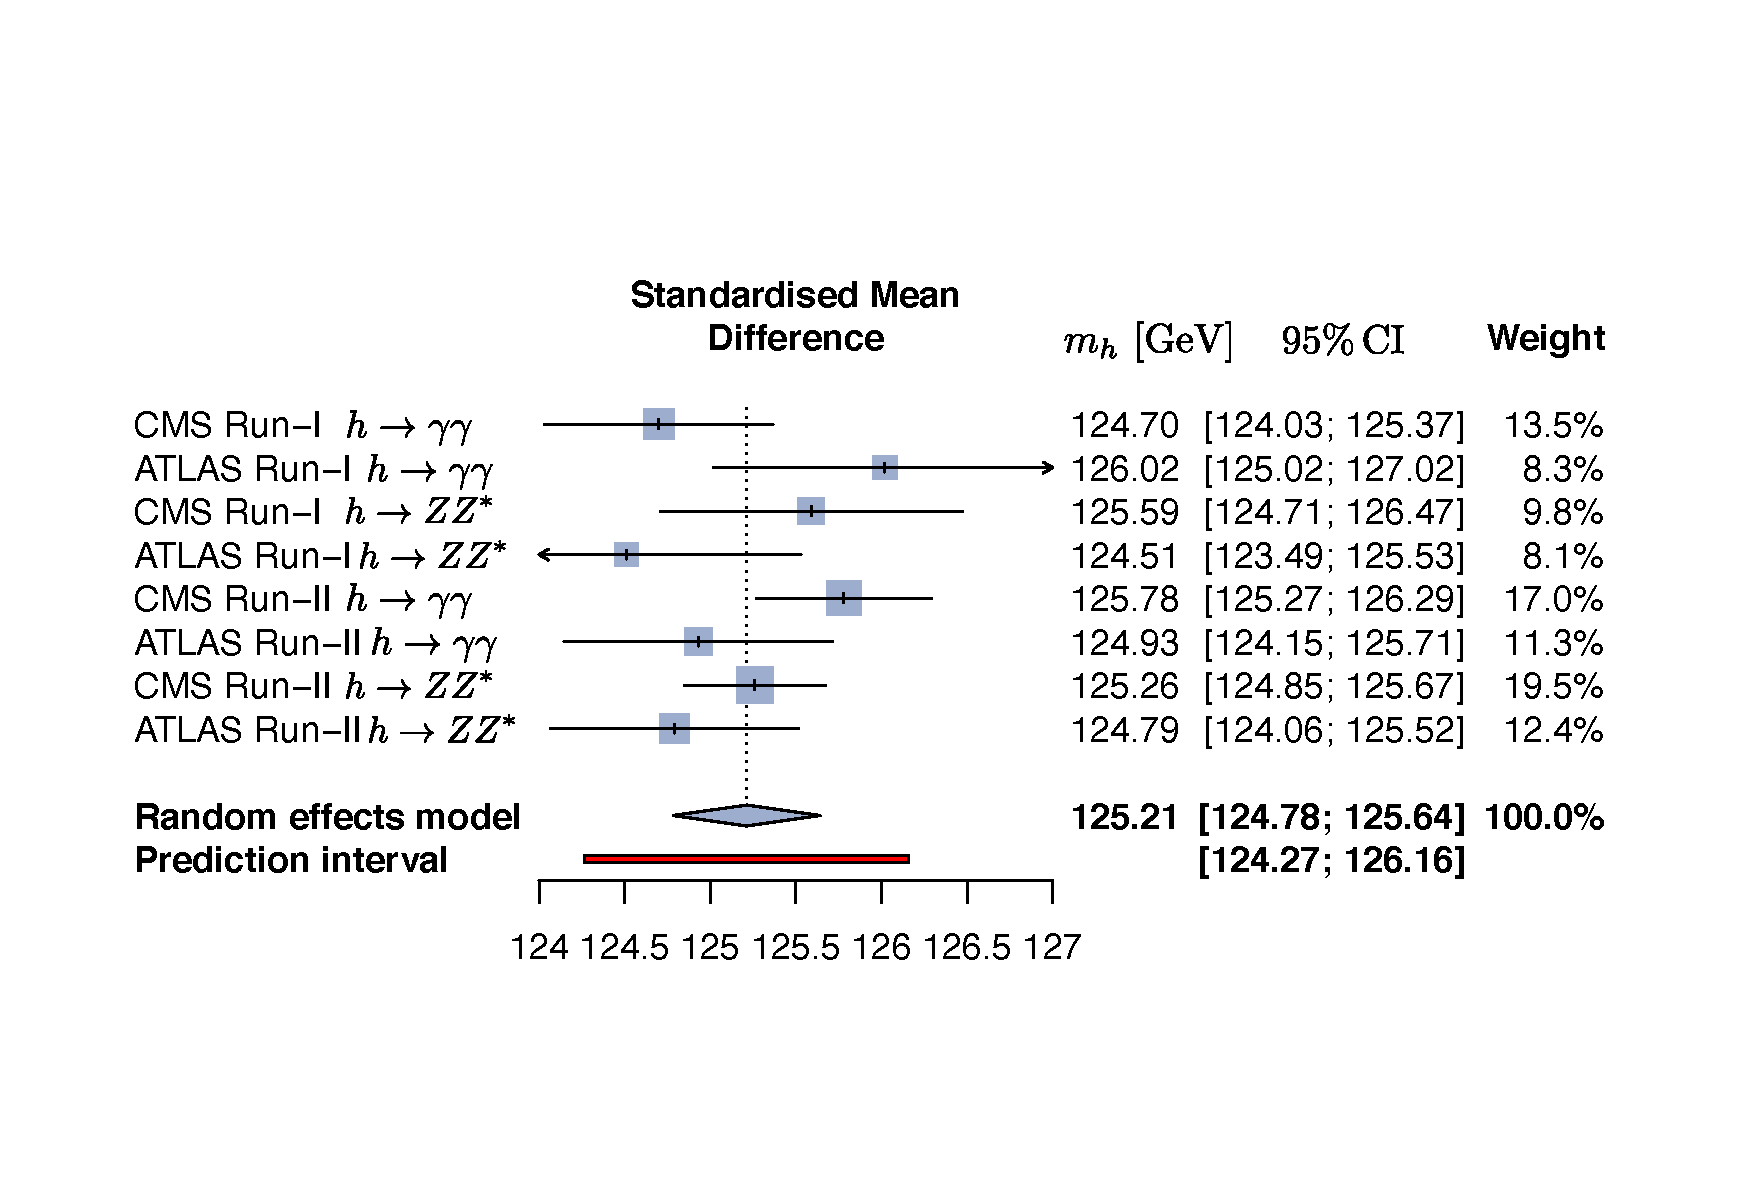
\includegraphics[width=1.\textwidth]{figures/foreest_pllot_higgs_mass}
		\caption{A meta analysis preformed to combine all the measurements of the Higgs mass from Run-I and Run-II, the combined result was obtained from pooling all of the studies using the random effects model method.\label{fig:meta_mass} }
	\end{center}
\end{figure}
\subsection{Higgs full width}
The SM values of the Higgs boson full width is ~$\Gamma_h=4.1$ \GeV\, and it can be accessed in the LHC by looking at the ratio of on-shell versus off-shell Higgs production and decay to the $ZZ^{(*)}$ state, and $ZZ^{(*)}\to 4 \ell, 2 \ell 2 \nu$, namely
\begin{equation}
\frac{\sigma(gg \to h\to Z Z^*)}{\sigma(gg \to h^*\to Z Z)} = \kappa_g^2 \kappa_Z^2 \frac{4 m_Z^2}{m_h \Gamma_h},
\label{widthform}
\end{equation}
where the $\kappa$ here denote the ratio between the measured/ or modified coupling with the Higgs and the SM prediction, i.e.
\begin{equation}
\kappa_X := \frac{g_{XX h}}{g_{XXh}^{\SM}}.
\label{kappa}
\end{equation}
Which is commonly used in reporting experimental constrains/ measurements of the Higgs couplings, as in the next section~\autoref{sec:Higgscoupl}. We shall discuss the $\kappa$ formalism more in~\autoref{chap:HiggsEFT}. \\ We see from~\eqref{widthform} that if one fixes the coupling between the gluons and the $Z$ boson and the Higgs it is possible to access the full width directly.  Unfortunately, it is not possible to directly measure the Higgs full width at the LHC, as this requires full reconstruction of the collision event and study the recoil mass which is only possible at lepton colliders~\cite{DeBlas:2019qco,Banerjee:2021huv}. 
Alas, it is still possible to extract bounds on $\Gamma_h$ using ~\eqref{widthform}. ATLAS used this method to constrain the full width of the Higgs using Run-II data~\cite{ATLAS:2018jym}, while CMS has preformed the same analysis using Run-I and Run-II data combined~\cite{CMS:2019ekd}, the results are 95\% CL bounds of $\Gamma_h$
\begin{align}
\Gamma_h &< \SI{14.4}{\giga\electronvolt} \,\,\,\, (\text{ATLAS}) & \SI{0.08}{\giga\electronvolt} <&\Gamma_h < \SI{9.16}{\giga\electronvolt}  \,\,\,\, (\text{CMS}),
\end{align}
with the combined bound being  $\sim 3 \Gamma_h^{\SM}$. 
\subsection{Higgs spin and parity \label{higgscp}}
As we have seen in ~\autoref{Higgsmech}, the Higgs boson in a scalar and $\mathcal{CP}$ even ($J^p= 0^+$) in the SM. However, the discovery of  a peak in the $m_\gamma \gamma$ distribution, would not automatically imply that the particle discovered is scalar, it could be a spin-$2$ boson, or a pseudoscalar  ($J^p= 0^-$). In order to study the $J^p$ properties of the Higgs, one needs to examine the differential distributions of angular variables such as rapidity~$y$ or transverse momentum~$\pt$. Both ATLAS and CMS collaborations studied using Run-I data the angular distributions of the Higgs decays $ h \to ZZ^*$, $h \to W W^*$ and $ h \to \gamma$. Then test the alternative hypothesis for $J^p$ against the SM~\cite{ATLAS:2015zhl,CMS:2014nkk}. As seen in~\autoref{fig:jcphiggs}, showing CMS results, that the SM ~$0^+$ hypothesis is favoured at $ >99.9\%$ CL.  
\begin{figure}[htb!]
	\begin{center}
		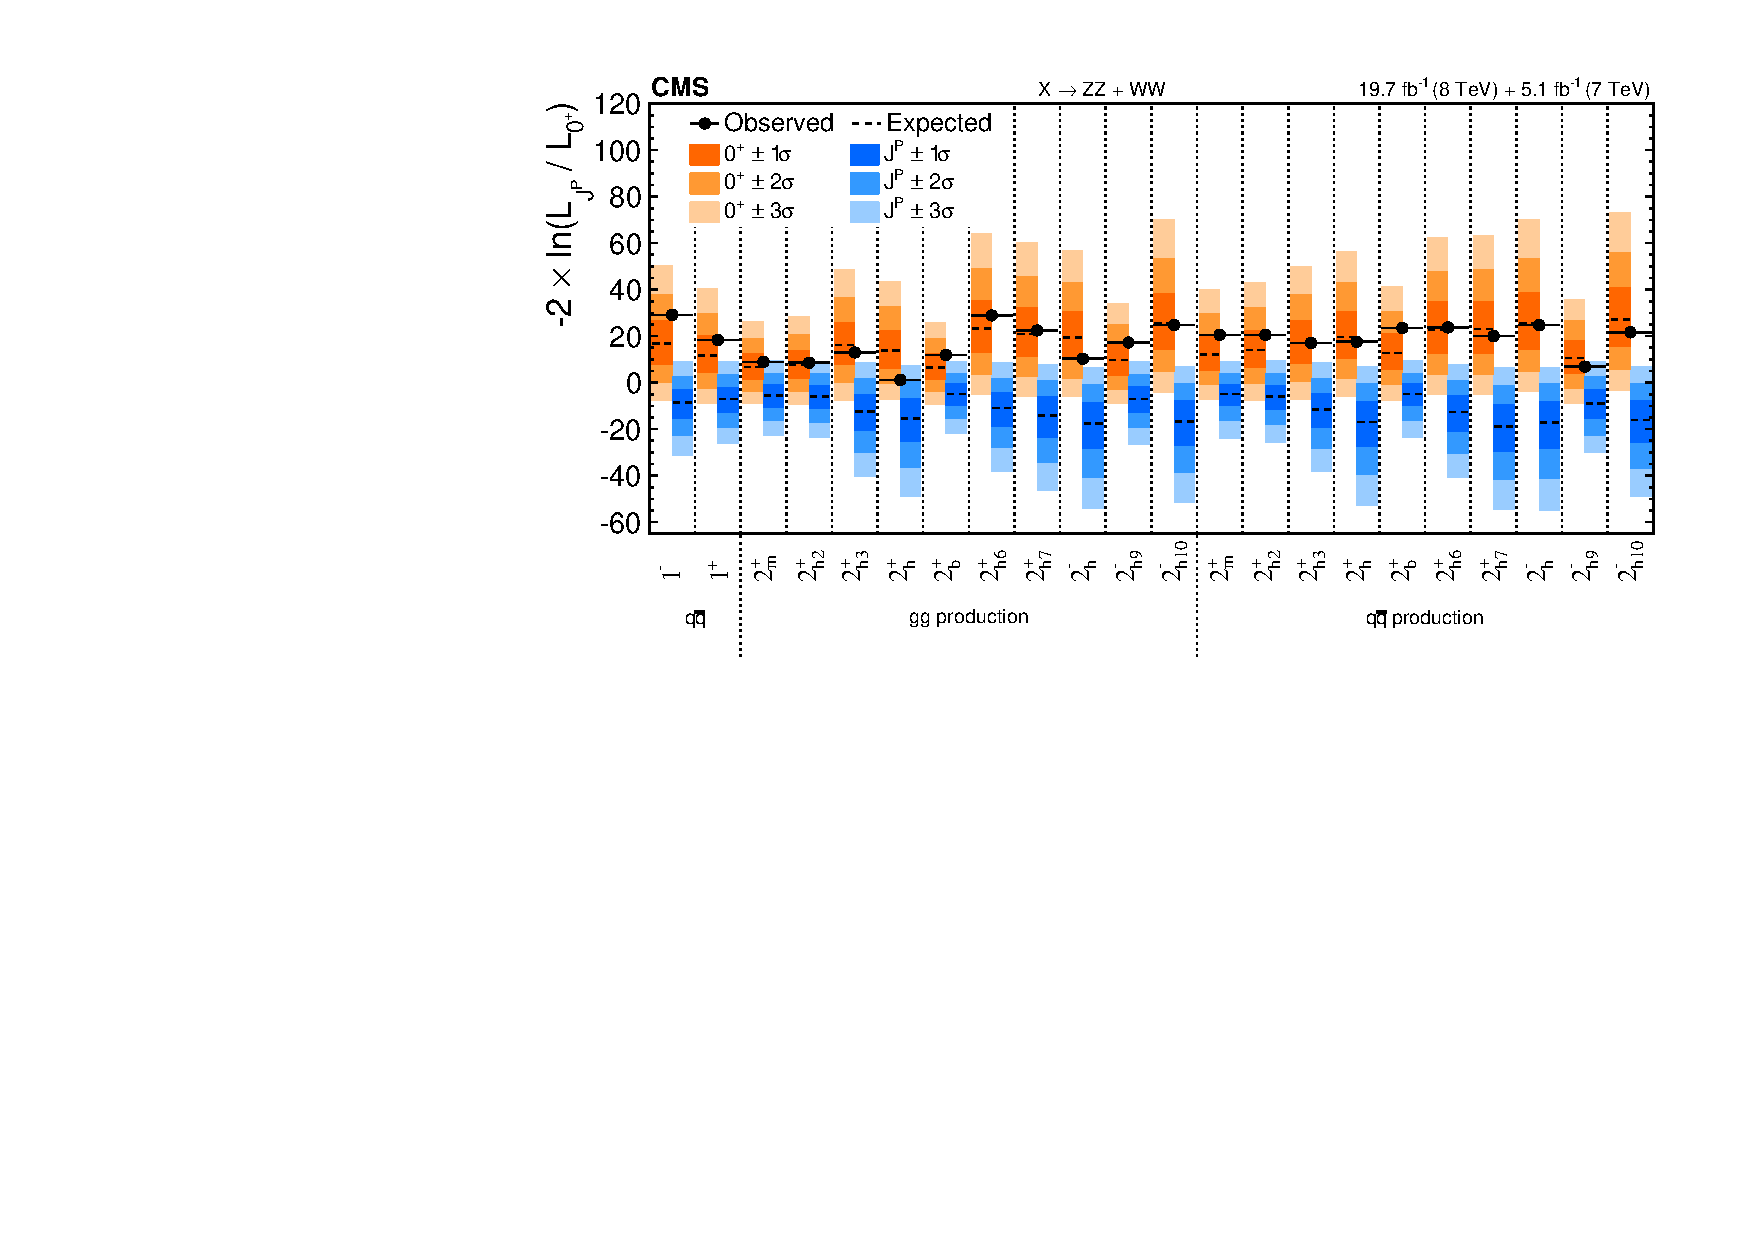
\includegraphics[width=1\textwidth]{figures/Higgs_results/CMS-HIG-14-018_Figure_018}
		\caption{The test-statistic distributions for the SM Higgs hypothesis versus other $J^p$ hypothesises in the $x$ axis. The hypothesis testing was conducted using the  $ h \to ZZ^*$, $h \to W W^*$  final-states. The SM hypothesis is indicated in orange, while the alternatives are in blue. Measurements are indicated in black points. This plot is from the CMS collaboration~\cite{CMS:2014nkk}}	
		\label{fig:jcphiggs}
	\end{center}
\end{figure}
\section{Measurements of Higgs rates and couplings \label{sec:Higgscoupl} }
\subsection{Higgs cross-sections}
\par The total inclusive Higgs cross-section has been measured using the the final states $ h \to \gamma \gamma$ and $ h\to Z Z^* \to 4 \ell$. and their combinations.  The measurements has been done at the three energies the LHC was operating at: 7 TeV, 8 TeV ~\cite{CMS:2015zpx} and 13 TeV~\cite{TheATLAScollaboration:2015uuh,CMS:2018gwt,CMS:2021ugl} and combined with more data and compared to the SM prediction as show in~\cite{ATLAS:2019mju}. As shown in~\autoref{fig:xstothiggs}, the measured inclusive cross-section is in agreement with the SM prediction across al of the LHC operation energies.
\begin{figure}[htb!]
	\begin{center}
		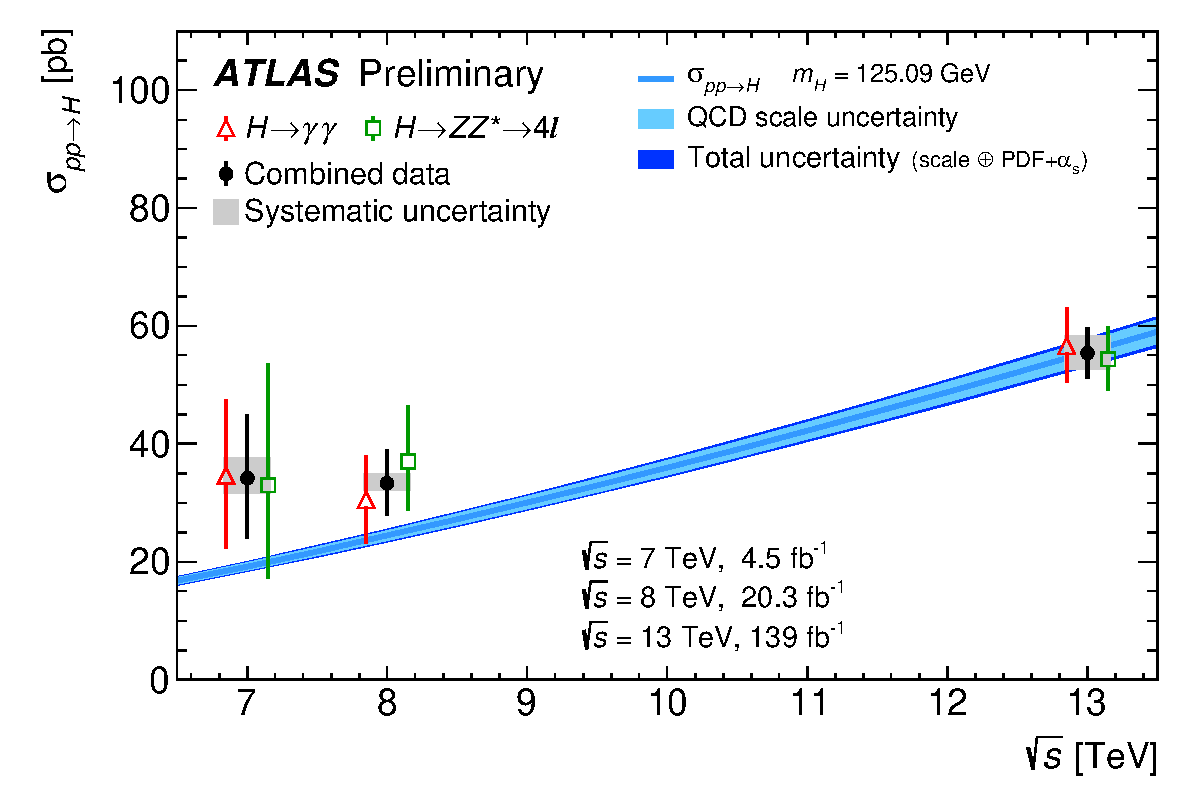
\includegraphics[height=0.35\textheight]{figures/Higgs_results/fig_01}
		\caption{The total inclusive cross-section measurements by ATLAS collaboration~\cite{ATLAS:2019mju} for $7$, $8$ and $13$ TeV using  $ h \to \gamma \gamma$ and $ h\to Z Z^* \to 4 \ell$. channels and their combination (black points) compared to the SM prediction with the  uncertainties shown as blue line with light and dark blue bands for QCD scale uncertainties and total uncertainties, respectively. }	
		\label{fig:xstothiggs}
	\end{center}
\end{figure}
%\FloatBarrier
\par In addition to the inclusive cross-section measurements,  differential cross-sections of the Higgs has been measured for $\pt$ and  $y$ as we have seen in~\autoref{higgscp} for Higgs's $J^p$ determination. Additional,  the differential cross-sections for other variables have been measured, and they include $N_{jets}, \pt^{jet}, m_{jj},\delta \phi_{jj]}$ and others using the channels $ h \to ZZ^*$, $h \to W W^*$ and $ h \to \gamma$. The most recent results using the full Run-II data can be found in Refs.~\cite{CMS:2018gwt,ATLAS:2019jst,ATLAS:2019mju,CMS:2019chr}.  
\par In addition to the total inclusive cross-section, a collection of measurements of Higgs production and decay rates has been carried out by both ATLAS and CMS. These measurements also carried out in , what is known as Standard Template Cross-Sections~(STXS) framework.The STXS's are fiducial cross-sections in exclusive phase-space regions or bins separately per Higgs boson production channel. They have the advantage of standardisation of cuts and final results such that measurements could be easily combined across analyses. More details about the STXS framework can be found in the reports of  LHC Higgs cross-sections working group~(LHCHXSWG) cf.~\cite{Berger:2019wnu}.  In~\autoref{table:resHiggsExp} I summarise the state-of-art measurements of the Higgs rates separated into production and decay channels using the total LHC Run-II data from ATLAS and CMS experiments. Additionally, I give the HL-LHC projections from CMS experiment as a comparison. The results in this table are written in terms of the signal strength, which is directly extracted from measuring the number of events dividing them by the standard model,
\begin{equation}
	\mu_{\mathrm{Exp}} := \frac{ \sigma \cdot \mathcal{B}}{ \sigma^{\SM} \cdot \mathcal{B}^{\SM}}.
\end{equation}
\newpage
\begingroup
\thispagestyle{plain}
\begin{table}[htb!]
\centering
\vspace{-1 cm}
 \footnotesize{ 
	{\renewcommand{\arraystretch}{0.75 }%
\begin{tabular}{clccc}
\toprule
\toprule
\multirow{5}{*}{ {\normalsize Production}}  &\multirow{5}{*}{ {\normalsize Decay}}&\multicolumn{2}{c}{ $\mu_{\mathrm{Exp}} \pm \delta \mu_{\mathrm{Exp}}$  (symmetrised)} &\multirow{5}{*}{ {\normalsize Ref.}} \\
%\cmidrule(r){3-4}
&   & { \bf     \scriptsize           LHC Run-II}&{ \bf  \scriptsize HL-LHC}&   \\
\cmidrule(r){3-4}
&   & { \scriptsize                   CMS $137 \, \mathrm{fb}^{-1} $}&  \multirow{2}{*}{CMS $3 \, \mathrm{ab}^{-1}$}&   \\
&   &  { \CG \scriptsize                   ATLAS $139 \, \mathrm{fb}^{-1} $} & &  \\
\midrule
\midrule
\multirow{ 13}{*}{ \normalsize ggF}         & \multirow{2}{*}{$h\to \gamma  \gamma$} & { \scriptsize                  $0.99 \pm 0.12$}& \multirow{2}{*}{$1.000\pm 0.042$}& \multirow{2}{*}{\cite{ATLAS:2020qdt,CMS:2021kom,CMS-PAS-FTR-18-011}}\\
                                           &                                                          &{ \scriptsize                   \CG $1.030 \pm 0.110$}&& \\ 
                                           \cmidrule(r){2-5}
                                           %%%%%%
                                    &  \mr{$h\to Z Z^*$}          & { \scriptsize                  $0.985 \pm 0.115$}&\multirow{2}{*}{$1.000 \pm 0.040$}&\multirow{7}{*}{\cite{ATLAS:2020qdt,CMS:2020gsy,CMS-PAS-FTR-18-011}}  \\
                                     &                                                      &{ \scriptsize                   \CG $0.945 \pm 0.105$}&& \\
                                     \cmidrule(r){2-4}
                                       %%%%%%
                                    &\mr{ $h\to W W^*$}         & { \scriptsize                  $1.285 \pm 0.195$} &\mr{ $1.000 \pm 0.037$} &\\
                                    & &                                            { \scriptsize                   \CG$1.085 \pm 0.185$} & &\\
                                                                         \cmidrule(r){2-4}
                                     %%%%%%
                                    &\mr{ $h\to \tau^+\tau^- $ }         & { \scriptsize                  $0.385 \pm 0.385$} &\mr{ $1.000 \pm 0.055$} &\\
                                 & &                                            { \scriptsize                   \CG$1.045 \pm 0.575$} & &\\
                                 \cmidrule(r){2-5}
                                 %%%%%%

                                  &\mr{ $h\to  b \bar b$  }      & { \scriptsize                 $2.54 \pm 2.44$} &\mr{ $1.000 \pm 0.247$} &\mr{\cite{CMS:2020gsy,CMS-PAS-FTR-18-011}}\\
                               & &                                            { \scriptsize                   \CG--} & &\\
                                 \cmidrule(r){2-5}
                               %%%%%%  %%%%%%   %%%%%%
                                  &\mr{ $h\to  \mu^+ \mu^-$  }      & { \scriptsize      $0.315 \pm 1.815$} &\mr{ $1.000 \pm 0.138$} &\mr{\cite{CMS:2020gsy,CMS-PAS-FTR-18-011} }\\
& &                                            { \scriptsize                   \CG--} & &\\
%%%%%%  %%%%%%   %%%%%%                               
\midrule
\midrule
%\crowcolor
\multirow{13}{*}{ \normalsize VBF}      
                                     %%%%%%
										&\mr{ $h\to \gamma  \gamma$ }         & { \scriptsize                  $1.175 \pm 0.335$ } &\mr{ $1.000 \pm 0.128$} & \mr{\cite{ATLAS:2020qdt,CMS:2021kom,CMS-PAS-FTR-18-011}}\\
										& &                                           { \scriptsize                   \CG$1.325 \pm 0.245$} & &\\
\cmidrule(r){2-5}
%%%%%%                                   
                                     &\mr{$h\to Z Z^*$ }         & { \scriptsize                  $0.62 \pm 0.41$ } &\mr{ $1.000 \pm 0.134$} & \multirow{7}{*}{\cite{ATLAS:2020qdt,CMS:2020gsy,CMS-PAS-FTR-18-011}}\\
                                    & &                                            { \scriptsize                   \CG$1.295 \pm 0.455$} & &\\
                                                                                             \cmidrule(r){2-4}
%%%%%%

                                   &\mr{$h\to W W^*$}         & { \scriptsize                  $0.65 \pm 0.63$ } &\mr{ $1.000 \pm 0.073$} & \\
                                    & &                                            { \scriptsize                   \CG$0.61 \pm 0.35$} & &\\
 \cmidrule(r){2-4}
%%%%%%0
                                   &\mr{$h\to \tau^+\tau^- $}         & { \scriptsize                  $1.055 \pm 0.295$ } &\mr{ $1.000 \pm 0.044$} & \\
& &                                            { \scriptsize                   \CG$1.17 \pm 0.55$} & &\\
\cmidrule(r){2-5}
%%%%%%0                                    
                                    &\mr{$h\to  b \bar b$}         & { \scriptsize                   -- } &\mr{--} & \mr{\cite{ATLAS:2020qdt} }\\
                                    & &                                            { \scriptsize                   \CG$3.055 \pm 1.645$} & &\\
                                    
                                  \cmidrule(r){2-5}
 %%%%%%  %%%%%%   %%%%%%
 &\mr{ $h\to  \mu^+ \mu^-$  }      & { \scriptsize               $3.325 \pm 8.075$} &\mr{ $1.000 \pm 0.540$} &\mr{ \cite{CMS-PAS-FTR-18-011}}\\
 & &                                            { \scriptsize                   \CG--} & & \\                                   
\midrule
\midrule
\multirow{10}{*}{ \normalsize  $t\bar t h$} 
%%%%%%0                                    
&\mr{ $h\to \gamma  \gamma$}         & { \scriptsize                $1.43 \pm 0.30$ } &\mr{$1.000 \pm 0.094$} & \mr{ \cite{ATLAS:2020qdt,CMS:2021kom,CMS-PAS-FTR-18-011} }\\
& &                                            { \scriptsize                   \CG$0.915 \pm 0.255$} & &\\

\cmidrule(r){2-5}

                                    
%%%%%%0                                    
&\multirow{3}{*} { $h\to V V^*$   }         & { \scriptsize              $0.64 \pm 0.64$({\color{Mahogany}$ZZ^*$}) } &{ \scriptsize   $1.000 \pm 0.246$ ({\color{Mahogany}$ZZ^*$}) } & \multirow{8}{*}{\cite{ATLAS:2020qdt,CMS:2020gsy,CMS-PAS-FTR-18-011}}  \\
& &                                            { \scriptsize                   $0.945\pm 0.465$ ({\color{Mahogany} $W W^*$})} & { \scriptsize   $1.000 \pm 0.097$ ({\color{Mahogany} $W W^*$})} &\\
& &                                            { \scriptsize                   \CG $1.735 \pm 0.545$} & { \scriptsize   --}&\\
\cmidrule(r){2-4}                                    

&\mr{$h\to \tau^+\tau^- $}         & { \scriptsize                $0.845 \pm 0.705$} &\mr{ $1.000 \pm 0.149$} & \\
& &                                            { \scriptsize                   \CG $1.27 \pm 1.0$} & &\\
\cmidrule(r){2-4}                                    

&\mr{ $h\to  b \bar b$  }         & { \scriptsize                 $1.145 \pm 0.315$} &\mr{ $1.000 \pm 0.116$} & \\
& &                                            { \scriptsize                   \CG $0.795 \pm 0.595$} & &\\                                                        
\midrule
\midrule
\multirow{9}{*}{ \normalsize $Vh$}        

                      
&\mr{ $h\to \gamma  \gamma$  }         & { \scriptsize   $0.725 \pm 0.295$ } &{ \scriptsize   $1.000 \pm 0.233$ ({\color{Mahogany}$Zh$}) } & \multirow{2}{*}{ \cite{ATLAS:2020qdt,CMS:2021kom,CMS-PAS-FTR-18-011}  }  \\
& &                                            { \scriptsize                   \CG $1.335 \pm 0.315$} & { \scriptsize   $1.000 \pm 0.139$ ({\color{Mahogany} $W^\pm h$})} &\\
\cmidrule(r){2-5}           
%%%%%%0              
                                    
&\mr{ $h\to Z Z^*$    }         & { \scriptsize   $1.21 \pm 0.85$ } &{ \scriptsize   $1.000 \pm 0.786$ ({\color{Mahogany}$Zh$}) } & \multirow{2}{*}{ \cite{ATLAS:2020qdt,CMS:2020gsy,CMS-PAS-FTR-18-011}  }  \\
& &                                            { \scriptsize                   \CG $1.635 \pm 1.025$} & { \scriptsize   $1.000 \pm 0.478$ ({\color{Mahogany} $W^\pm h$})} &\\
\cmidrule(r){2-5}           
%%%%%%0                                         
                                  
 &\mr{ $h\to W W^*$    }         & { \scriptsize   $1.850\pm 0.438$ } &{ \scriptsize   $1.000 \pm 0.184$ ({\color{Mahogany}$Zh$}) } & \multirow{2}{*}{  \cite{CMS:2021ixs,CMS-PAS-FTR-18-011} }  \\
 & &                                            { \scriptsize                   \CG --} & { \scriptsize   $1.000 \pm 0.138$ ({\color{Mahogany} $W^\pm h$})} &\\
 \cmidrule(r){2-5}           
 %%%%%%0                                                                                                            
 &\mr{$h\to  b \bar b$      }         & { \scriptsize  -- } &{ \scriptsize   $1.000 \pm 0.065$ ({\color{Mahogany}$Zh$}) } & \multirow{2}{*}{  \cite{ATLAS:2020qdt,CMS-PAS-FTR-18-011} }  \\
& &                                            { \scriptsize                   \CG $1.025 \pm 0.175$} & { \scriptsize   $1.000 \pm 0.094$ ({\color{Mahogany} $W^\pm h$})} &\\

%%%%%%0                                        
                                    
\midrule
\midrule
\multirow{2}{*}{ \normalsize $Zh$ { \scriptsize {\color{Mahogany} CMS     }   }}    & $h\to \tau^+\tau^- $ & $1.645 \pm 1.485$&\multirow{5}{*}{--} &\multirow{5}{*}{ \cite{CMS:2020gsy} }  \\
& $h\to  b \bar b$       &$0.94 \pm 0.32$&&\\                         
 \cmidrule(r){2-3}    
\multirow{2}{*}{ \normalsize $W^\pm h${ \scriptsize {\color{Mahogany} CMS     }   }}           & $h\to \tau^+\tau^- $ &$3.08 \pm 1.58$&&\\
& $h\to  b \bar b$      & $1.28 \pm 0.41$&&\\                  
\midrule
\midrule
\end{tabular}
}
}
\caption{The experimental single Higgs production and decay rates measurements from the  complete  data of LHC Run II and projections for the HL-LHC. The uncertainties were symmetrised here. The table is published in~\cite{Alasfar:2022zyr}.  }
\label{table:resHiggsExp}
\end{table} 
\endgroup
\FloatBarrier
\subsection{Constraints on Higgs couplings}
The measurements of the Higgs rates and their combination (also including STXS) have been used to set bounds on the Higgs couplings, the most recent bounds - as this thesis being written - have been reported by ATLAS using the Higgs inclusive rates and STXS for the full Run-II data~\cite{ATLAS2021vrm}, and  by CMS using Higgs rates shown in ~\autoref{table:resHiggsExp} ~\cite{CMS:2020gsy}. In~\autoref{fig:couplings-bound}, I present the aggregation the ATLAS and CMS bounds on the Higgs coupling modifiers in the $\kappa$ formalism defined in eq.~\eqref{kappa}. The aggregation of these bounds was preformed using the method described in~\cite{BHHR} assuming there is no correlation between ATLAS and CMS measurements.  
\begin{figure}[htb!]
	\begin{center}
		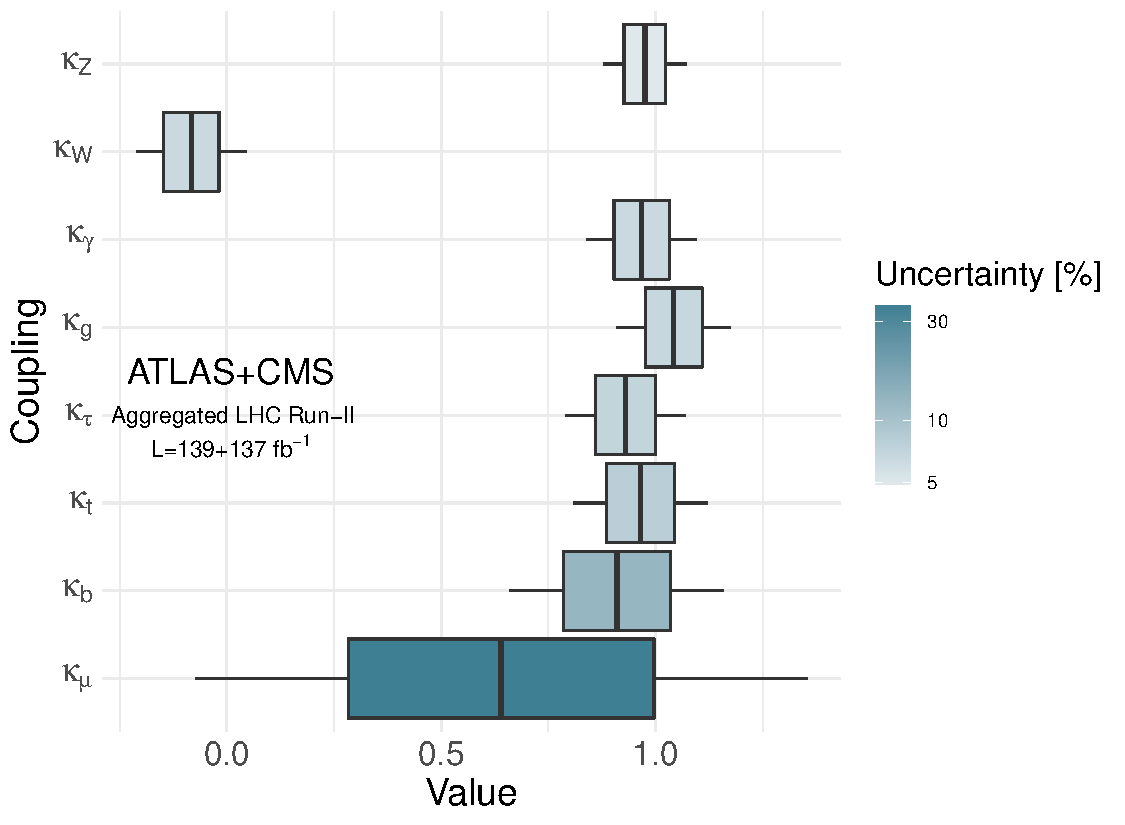
\includegraphics[height=0.35\textheight]{figures/agg_higgs_couplings}
		\caption{Meta analysis aggravating the most recent bounds from ATLAS~\cite{ATLAS2021vrm} and CMS~\cite{CMS:2020gsy} on the Higgs couplings modifiers $\kappa$.   }	
		\label{fig:couplings-bound}
	\end{center}
\end{figure}
\par Examining~\autoref{fig:couplings-bound}, we observe that the bounds on the Higgs boson's coupling to the gauge boson, including the effective couplings to $\gamma$ and $g$, as well as the couplings to the third-generation fermions are in few percent within the SM prediction. The bounds on the coupling to the $W$ seems to  favour a negative value in CMS fits, due to the channel used to constraint it $ h \to WW$ which depends on $ \kappa_W^2$, thus making the best fit value of $ \sim -1$ within the SM prediction. An independent analysis on the relative signs of $\kappa_W$ and $\kappa_t$ was preformed using $th$ process in Ref.~\cite{CMS:2018jeh}
\subsection{Anomalous couplings }
to measure $HVV$ CMS used the same data for extraction of the $\Gamma_h$ to study this~\cite{CMS:2019ekd}
\newpage
\begin{figure}[t!]
	\begin{center}
		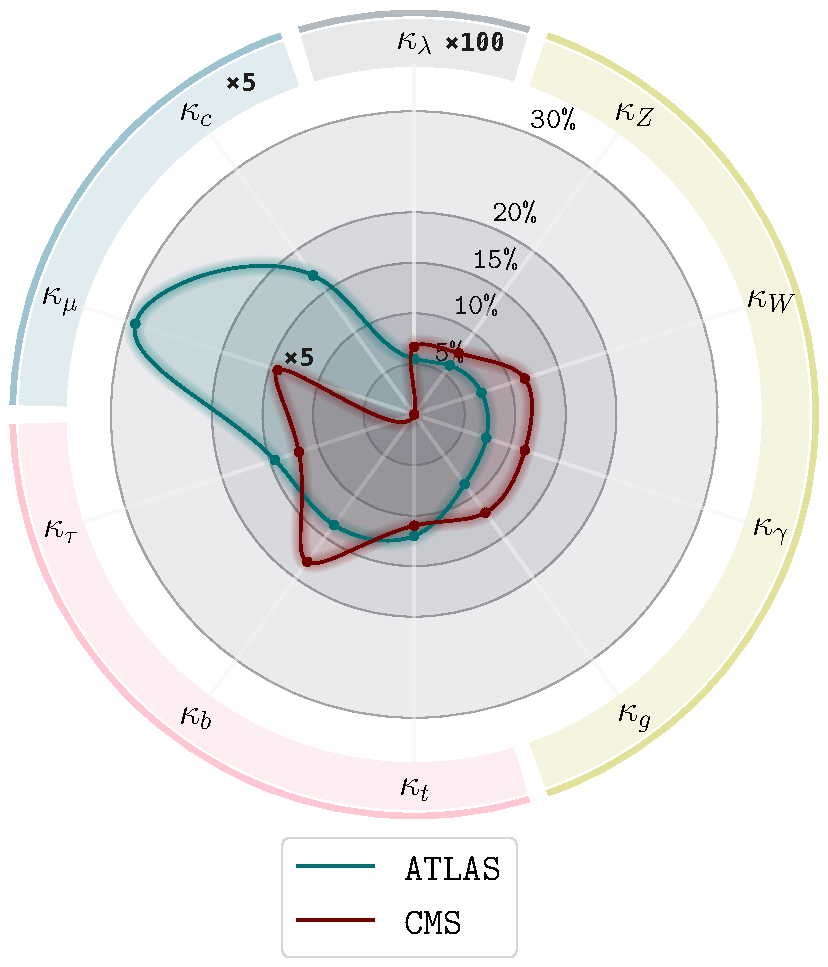
\includegraphics[width=12cm]{figures/Higgs_couplings_poster}
		\caption{ddd  \label{fig:higgs_kappa}}
	\end{center}
\end{figure}
\section{Challenges and outlook \label{sec:Higgscouplchallenge} }
%We also provide in this appendix the experimental measurements of the signal strengths at the LHC Run II and the CMS projections for the HL-LHC (scenario S2, see \cite{Cepeda:2019klc}) that we used in the fits in this paper. These inputs are summarised in table~\ref{table:resHiggsExp}.
       
        %!TEX encoding = UTF-8 Unicode
% !TeX spellcheck = en_GB
%%%%%%%%%%%%%%%%%%%%%%%%%%%%%%%%%%%%%%
\chapter{Higgs and effective field theories }\label{chap:HiggsEFT}
%%%%%%%%%%%%%%%%%%%%%%%%%%%%%%%%%%%%%%
\par The Standard Model (SM) has been concluded after the Higgs boson discovery~\cite{ATLAS:2012yve,CMS:2012qbp}, followed by its extensive characterisation by the ATLAS and CMS experiments including its general properties~\cite{ATLAS:2015yey,ATLAS:2018tdk,CMS:2017dib,CMS:2020xrn,ATLAS:2018jym,CMS:2019ekd,ATLAS:2015zhl, CMS:2014nkk},  cross-sections~\cite{CMS:2018gwt,ATLAS:2019jst,ATLAS:2019mju,CMS:2019chr} and couplings to electroweak and heavier fermions~\cite{ATLAS2021vrm,CMS:2020gsy}. Nonetheless, there are many open questions regarding the nature of the Higgs boson, which are left unanswered. This includes the shape of Higgs boson potential, its coupling to light quarks and the hierarchy problem. Answering these questions opens space for extending the SM by New Physics (NP) degrees of freedom.
\par In order to make the search for NP more accessible and model-agnostic, we revert to~\textbf{effective field theories}~(EFT), one of the most perspicacious concepts of quantum field theory. In the EFT framework, the interactions mediated by NP at the small scale of arbitrary complexity can be systematically simplified by approximating these interactions via integrating the UV degrees of freedom, leaving numerable operators consisting of higher dimensional operator consisting of SM fields, which are added to the SM. 
%The premise of EFTs can be simply illustrated in~\autoref{fig:eft}.  For example, the LHC might not be able to resolve the UV degrees of freedom at their scale~$\Lambda$; rather, one can only observe the effective interactions they mediate. These new interactions depend on a set of free parameters known as~\textbf{Wilson coefficients}, which would be constrained or set from experiments. 
These ``phenomenological Lagrangians'', as called by Weinberg~\cite{WEINBERG1979327}, are not necessarily renormalisable but still allow for robust predictions that can be tested at colliders, including higher-order effects. \\
This chapter is organised as follows:  In ~\autoref{sec:smeft}, the Higgs sector of Standard Model effective field theory~(SMEFT) is presented along with the parametrisation of single and di-Higgs rates in terms of the SMEFT Wilson coefficients. In contrast to the SMEFT formalism, \autoref{sec:chiral} will present a non-linear EFT formalism known as the EW Chiral Lagrangian~(EWChL) or the  Higgs effective field theory (HEFT). Finally, I will conclude this chapter in~\autoref{sec:concefts}.
%%%%%%%%%
\section{The Higgs boson and Standard Model effective field theory \label{sec:smeft}}
\par The idea behind the Standard Model effective field theory is to preserve the SM symmetries and fields. In particular, the Higgs boson $h(x)$ is assumed to originate from the doublet $\phi$, like the SM.  New operators of higher mass dimension are added to dimension-four SM operators. These new operators consist of the SM fields and obey its symmetries. Although these operators are not renormalisable, they are, nonetheless, predictive.
\par From simple dimensional analysis, it is known that higher dimensional operators need to contain an inverse mass with some power $p=4-d$ in the couplings. Therefore, it is not needed to use the infinite number of the Wilson coefficients~$C_i$ when fitting to experimental measurements. Since, the higher dimensional operators are suppressed by higher powers of the UV scale $\Lambda$, hence their effect can be neglected. For example, if the NP scale is set to  $\Lambda =1$, then the effects of dimension-six operators will be at the per cent level. At the same time, dimension-eight operators will have effects of order~$\sim10^{-4}$, allowing to ignore the dimension-eight and higher operators in the majority of the LHC studies.  Regarding dimension-five, there is only one operator called the Weinberg operator~\cite{PhysRevLett.43.1566}, which does not have a considerable Higgs phenomenology. Hence, I shall be discussing SMEFT with dimension-six operators only as  they have the most prominent collider phenomenology~\cite{BUCHMULLER1986621,Hagiwara:1993ck}, for studies on Higher-dimensional SMEFT operators cf.~\cite{Lehman:2014jma,Lehman:2015coa,Henning:2015alf,Aguilar-Saavedra:2010uur}. \\ The SMEFT Lagrangian up to dimension-six operators is given by
%%%%%%%%%%
\begin{equation}
	\mathcal{L}_{\mathrm{SMEFT}}^{d=6}=\mathcal{L}_{\SM} + \frac{1}{\Lambda^2}\sum_i C_i  {\cal O}_i.
	\label{smeftdim6}
\end{equation}
%%%%%%%%%%%
\begin{table}
	\begin{center}
		\footnotesize
			\vspace{-.35cm}
		\hspace{-2.7 cm}
		\begin{minipage}[t]{4.6cm}
			\renewcommand{\arraystretch}{1.5}
			\begin{tabular}[t]{c|c}
				\multicolumn{2}{c}{$X^3$} \\
				\toplinetwo
				$\mathcal{O}_G$                & $f^{ABC} G_\mu^{A\nu} G_\nu^{B\rho} G_\rho^{C\mu} $ \\
				%
				$\mathcal{O}_{\widetilde G}$          & $f^{ABC} \widetilde G_\mu^{A\nu} G_\nu^{B\rho} G_\rho^{C\mu} $ \\
				%
				$\mathcal{O}_W$                & $\epsilon^{IJK} W_\mu^{I\nu} W_\nu^{J\rho} W_\rho^{K\mu}$ \\ 
				%
				$\mathcal{O}_{\widetilde W}$          & $\epsilon^{IJK} \widetilde W_\mu^{I\nu} W_\nu^{J\rho} W_\rho^{K\mu}$ \\
			\end{tabular}
		\end{minipage}
		%
		%
		%
		%
		\begin{minipage}[t]{4.6cm}
			\renewcommand{\arraystretch}{1.5}
			\begin{tabular}[t]{c|c}
				\multicolumn{2}{c}{Pure Higgs} \\
				\toplinetwo
				$\mathcal{O}_{\phi\Box}$ & $(\phi^\dag \phi)\Box(\phi^\dag \phi)$ \\
				%
				$\mathcal{O}_{\phi D}$   & $\ \left(\phi^\dag D_\mu \phi\right)^* \left(\phi^\dag D_\mu \phi\right)$ \\
				%
				$\mathcal{O}_\phi$       & $(\phi^\dag \phi)^3$ 
			\end{tabular}
		\end{minipage}
		%
		%
		\begin{minipage}[t]{2.7cm}
			
			\renewcommand{\arraystretch}{1.5}
			\begin{tabular}[t]{c|c}
				\multicolumn{2}{c}{$ \psi^2\phi^3 + \hbox{h.c.}$} \\
				\toplinetwo
				$\mathcal{O}_{e\phi}$           & $(\phi^\dag \phi)(\bar l_p e_r \phi)$ \\
				%
				$\mathcal{O}_{u\phi}$          & $(\phi^\dag \phi)(\bar q_p u_r \widetilde \phi )$ \\
				%
				$\mathcal{O}_{d\phi}$           & $(\phi^\dag \phi)(\bar q_p d_r \phi)$\\
			\end{tabular}
		\end{minipage}
		
		\vspace{0.25cm}
				\hspace{-2.7 cm}
		\begin{minipage}[t]{4.6cm}
			\renewcommand{\arraystretch}{1.5}
			\begin{tabular}[t]{c|c}
				\multicolumn{2}{c}{$X^2\phi^2$} \\
				\toplinetwo
				$\mathcal{O}_{\phi G}$     & $\phi^\dag \phi\, G^A_{\mu\nu} G^{A\mu\nu}$ \\
				%
				$\mathcal{O}_{\phi\widetilde G}$         & $\phi^\dag \phi\, \widetilde G^A_{\mu\nu} G^{A\mu\nu}$ \\
				%
				$\mathcal{O}_{\phi W}$     & $\phi^\dag \phi\, W^I_{\mu\nu} W^{I\mu\nu}$ \\
				%
				$\mathcal{O}_{\phi\widetilde W}$         & $\phi^\dag \phi\, \widetilde W^I_{\mu\nu} W^{I\mu\nu}$ \\
				%
				$\mathcal{O}_{\phi B}$     & $ \phi^\dag \phi\, B_{\mu\nu} B^{\mu\nu}$ \\
				%
				$\mathcal{O}_{\phi\widetilde B}$         & $\phi^\dag \phi\, \widetilde B_{\mu\nu} B^{\mu\nu}$ \\
				%
				$\mathcal{O}_{\phi WB}$     & $ \phi^\dag \tau^I \phi\, W^I_{\mu\nu} B^{\mu\nu}$ \\
				%
				$\mathcal{O}_{\phi\widetilde W B}$         & $\phi^\dag \tau^I \phi\, \widetilde W^I_{\mu\nu} B^{\mu\nu}$ 
			\end{tabular}
		\end{minipage}
		%
		%
		\begin{minipage}[t]{4.6cm}
			\renewcommand{\arraystretch}{1.5}
			\begin{tabular}[t]{c|c}
				\multicolumn{2}{c}{$\psi^2 X\phi+\hbox{h.c.}$} \\
				\toplinetwo
				$\mathcal{O}_{eW}$      & $(\bar l_p \sigma^{\mu\nu} e_r) \tau^I \phi W_{\mu\nu}^I$ \\
				%
				$\mathcal{O}_{eB}$        & $(\bar l_p \sigma^{\mu\nu} e_r) \phi B_{\mu\nu}$ \\
				%
				$\mathcal{O}_{uG}$        & $(\bar q_p \sigma^{\mu\nu} T^A u_r) \widetilde \phi \, G_{\mu\nu}^A$ \\
				%
				$\mathcal{O}_{uW}$        & $(\bar q_p \sigma^{\mu\nu} u_r) \tau^I \widetilde \phi \, W_{\mu\nu}^I$ \\
				%
				$\mathcal{O}_{uB}$        & $(\bar q_p \sigma^{\mu\nu} u_r) \widetilde \phi \, B_{\mu\nu}$ \\
				%
				$\mathcal{O}_{dG}$        & $(\bar q_p \sigma^{\mu\nu} T^A d_r) \phi\, G_{\mu\nu}^A$ \\
				%
				$\mathcal{O}_{dW}$         & $(\bar q_p \sigma^{\mu\nu} d_r) \tau^I \phi\, W_{\mu\nu}^I$ \\
				%
				$\mathcal{O}_{dB}$        & $(\bar q_p \sigma^{\mu\nu} d_r) \phi\, B_{\mu\nu}$ 
			\end{tabular}
		\end{minipage}
		%
		%
		\begin{minipage}[t]{2.7cm}
			\renewcommand{\arraystretch}{1.5}
			\begin{tabular}[t]{c|c}
				\multicolumn{2}{c}{$\psi^2\phi^2 D$} \\
				\toplinetwo
				$\mathcal{O}_{\phi l}^{(1)}$      & $(\phi^\dag i\overleftrightarrow{D}_\mu \phi)(\bar l_p \gamma^\mu l_r)$\\
				%
				$\mathcal{O}_{\phi l}^{(3)}$      & $(\phi^\dag i\overleftrightarrow{D}^I_\mu \phi)(\bar l_p \tau^I \gamma^\mu l_r)$\\
				%
				$\mathcal{O}_{\phi e}$            & $(\phi^\dag i\overleftrightarrow{D}_\mu \phi)(\bar e_p \gamma^\mu e_r)$\\
				%
				$\mathcal{O}_{\phi q}^{(1)}$      & $(\phi^\dag i\overleftrightarrow{D}_\mu \phi)(\bar q_p \gamma^\mu q_r)$\\
				%
				$\mathcal{O}_{\phi q}^{(3)}$      & $(\phi^\dag i\overleftrightarrow{D}^I_\mu \phi)(\bar q_p \tau^I \gamma^\mu q_r)$\\
				%
				$\mathcal{O}_{\phi u}$            & $(\phi^\dag i\overleftrightarrow{D}_\mu \phi)(\bar u_p \gamma^\mu u_r)$\\
				%
				$\mathcal{O}_{\phi d}$            & $(\phi^\dag i\overleftrightarrow{D}_\mu \phi)(\bar d_p \gamma^\mu d_r)$\\
				%
				$\mathcal{O}_{\phi u d}$ + h.c.   & $i(\widetilde \phi ^\dag D_\mu \phi)(\bar u_p \gamma^\mu d_r)$\\
			\end{tabular}
		\end{minipage}
		
		\vspace{0.25cm}
\hspace{-2.7 cm}
		
		\begin{minipage}[t]{4.95cm}
			\renewcommand{\arraystretch}{1.5}
			\begin{tabular}[t]{c|c}
				\multicolumn{2}{c}{$(\bar LL)(\bar LL)$} \\
				\toplinetwo
				$\mathcal{O}_{ll}$        & $(\bar l_p \gamma_\mu l_r)(\bar l_s \gamma^\mu l_t)$ \\
				%
				$\mathcal{O}_{qq}^{(1)}$  & $(\bar q_p \gamma_\mu q_r)(\bar q_s \gamma^\mu q_t)$ \\
				%
				$\mathcal{O}_{qq}^{(3)}$  & $(\bar q_p \gamma_\mu \tau^I q_r)(\bar q_s \gamma^\mu \tau^I q_t)$ \\
				%
				$\mathcal{O}_{lq}^{(1)}$                & $(\bar l_p \gamma_\mu l_r)(\bar q_s \gamma^\mu q_t)$ \\
				%
				$\mathcal{O}_{lq}^{(3)}$                & $(\bar l_p \gamma_\mu \tau^I l_r)(\bar q_s \gamma^\mu \tau^I q_t)$ 
			\end{tabular}
		\end{minipage}
		%
		%
		\begin{minipage}[t]{5.45cm}
			\renewcommand{\arraystretch}{1.5}
			\begin{tabular}[t]{c|c}
				\multicolumn{2}{c}{$(\bar RR)(\bar RR)$} \\
				\toplinetwo
				$\mathcal{O}_{ee}$               & $(\bar e_p \gamma_\mu e_r)(\bar e_s \gamma^\mu e_t)$ \\
				%
				$\mathcal{O}_{uu}$        & $(\bar u_p \gamma_\mu u_r)(\bar u_s \gamma^\mu u_t)$ \\
				%
				$\mathcal{O}_{dd}$        & $(\bar d_p \gamma_\mu d_r)(\bar d_s \gamma^\mu d_t)$ \\
				%
				$\mathcal{O}_{eu}$                      & $(\bar e_p \gamma_\mu e_r)(\bar u_s \gamma^\mu u_t)$ \\
				%
				$\mathcal{O}_{ed}$                      & $(\bar e_p \gamma_\mu e_r)(\bar d_s\gamma^\mu d_t)$ \\
				%
				$\mathcal{O}_{ud}^{(1)}$                & $(\bar u_p \gamma_\mu u_r)(\bar d_s \gamma^\mu d_t)$ \\
				%
				$\mathcal{O}_{ud}^{(8)}$                & $(\bar u_p \gamma_\mu T^A u_r)(\bar d_s \gamma^\mu T^A d_t)$ \\
				%
			\end{tabular}
		\end{minipage}

		\begin{minipage}[t]{4.95cm}
			\renewcommand{\arraystretch}{1.5}
			\begin{tabular}[t]{c|c}
				\multicolumn{2}{c}{$(\bar LL)(\bar RR)$} \\
				\toplinetwo
				$\mathcal{O}_{le}$               & $(\bar l_p \gamma_\mu l_r)(\bar e_s \gamma^\mu e_t)$ \\
				%
				$\mathcal{O}_{lu}$               & $(\bar l_p \gamma_\mu l_r)(\bar u_s \gamma^\mu u_t)$ \\
				%
				$\mathcal{O}_{ld}$               & $(\bar l_p \gamma_\mu l_r)(\bar d_s \gamma^\mu d_t)$ \\
				%
				$\mathcal{O}_{qe}$               & $(\bar q_p \gamma_\mu q_r)(\bar e_s \gamma^\mu e_t)$ \\
				%
				$\mathcal{O}_{qu}^{(1)}$         & $(\bar q_p \gamma_\mu q_r)(\bar u_s \gamma^\mu u_t)$ \\ 
				%
				$\mathcal{O}_{qu}^{(8)}$         & $(\bar q_p \gamma_\mu T^A q_r)(\bar u_s \gamma^\mu T^A u_t)$ \\ 
				%
				$\mathcal{O}_{qd}^{(1)}$ & $(\bar q_p \gamma_\mu q_r)(\bar d_s \gamma^\mu d_t)$ \\
				%
				$\mathcal{O}_{qd}^{(8)}$ & $(\bar q_p \gamma_\mu T^A q_r)(\bar d_s \gamma^\mu T^A d_t)$\\
			\end{tabular}
		\end{minipage}
		%
		%
		\begin{minipage}[t]{5.45 cm}
			\renewcommand{\arraystretch}{1.5}
			\begin{tabular}[t]{c|c}
				\multicolumn{2}{c}{$(\bar LR)(\bar L R)+\hbox{h.c.}$} \\
				\toplinetwo
				$\mathcal{O}_{quqd}^{(1)}$ & $(\bar q_p^j u_r) \epsilon_{jk} (\bar q_s^k d_t)$ \\
				%
				$\mathcal{O}_{quqd}^{(8)}$ & $(\bar q_p^j T^A u_r) \epsilon_{jk} (\bar q_s^k T^A d_t)$ \\
				%
				$\mathcal{O}_{lequ}^{(1)}$ & $(\bar l_p^j e_r) \epsilon_{jk} (\bar q_s^k u_t)$ \\
				%
				$\mathcal{O}_{lequ}^{(3)}$ & $(\bar l_p^j \sigma_{\mu\nu} e_r) \epsilon_{jk} (\bar q_s^k \sigma^{\mu\nu} u_t)$\\
				%
			 $\mathcal{O}_{ledq}$ & $(\bar l_p^j e_r)(\bar d_s q_{tj})$ 
			\end{tabular}
		\end{minipage}
	\end{center}
		\vspace{-.35cm}
	\caption{\label{warsaw}
	  Complete list of the dimension-six SMEFT operators in the Warsaw basis 
		\cite{Grzadkowski:2010es}. The $\mathcal{CP}$ violating operators contains the dual fields~$\widetilde X$. The flavour labels of the form $p,r,s,t$ on the $\mathcal{O}$ operators are suppressed on the left hand side of
		the tables.}
\end{table}
%%%%%%%%%%%
Phenomenological studies of EFTs with dimension-six operators primarily focus on using a set of complete and non-redundant ``basis''. This is since different effective operators will correspond to the same observables, e.g. same scattering amplitudes of SM particles.  This is the case if the operators can be related using equations of motion, Fierz transformations, integration by parts or field redefinitions. Thus leading to non-trivial and counter-intuitive relations between operators. Consequently, the construction of basis for the dimension-six SMEFT Lagrangian of eq.~\eqref{smeftdim6} is a cumbersome task. Such task has been accomplished by~\cite{Grzadkowski:2010es} recently forming what is known as the \textbf{Warsaw Basis}.  Another set of basis is the strongly-interacting light Higgs basis (SILH), initially proposed by~\cite{Giudice:2007fh}, before the Warsaw basis and completed in refs.~\cite{Contino:2013kra, Elias-Miro:2013eta}. A more recent set of basis has been published in~\cite{Gupta:2014rxa} using a subset of couplings characterising the interactions of mass eigenstates in the effective Lagrangian.\\
The complete $d=6$ SMEFT is described by 2499 independent parameters~\cite{Jenkins:2013zja,Jenkins:2013wua,Alonso:2013hga}. However, if one suppresses the flavour indices, assuming SMEFT is flavour universal, their inventory is significantly reduced. In the Warsaw basis, for example, assuming Baryon number conservation and dropping the flavour indices, one has only 59 operators, listed in~\autoref{warsaw}. It should be noted that all of the SMEFT basis will produce the same phenomenology, though the choice of basis is sometimes helpful in simplifying the analysis. In this thesis, I will focus on Warsaw basis.\\ 
\subsection{Single Higgs processes in SMEFT}
Single Higgs production and decay processes are modified at LO by a relatively long list of operators summarised in~eqs.~\eqref{box:smefthiggslo}, ~\eqref{box:smefthiggslo2} and~\eqref{box:smefthiggslo3}. Explicit formulae for the Higgs rates dependence on the Wilson coefficients of these operators can be found in~\cite{ATLAS:2019dhi}
\begin{tcolorbox}[title=SMEFT operators modifying Higgs rates at LO,
	title filled=false,
	colback=Mahogany!5!white,
	colframe=Mahogany ]
	Higgs operators
	\begin{align}
		C_{\phi D}, \ \mathcal{O}_{\phi \Box},\ \mathcal{O}_{\phi G}, \ \mathcal{O}_{\phi W},\ \mathcal{O}_{\phi B}, \ \mathcal{O}_{\phi W B},\ \mathcal{O}_{\phi l}^{(1)}, \nn \\
		\ \mathcal{O}_{\phi l}^{(3)}, \ \mathcal{O}_{\phi e},\ \mathcal{O}_{\phi q}^{(1)},\ \mathcal{O}_{\phi q}^{(3)}, \  \mathcal{O}_{\phi u}, \ \mathcal{O}_{\phi d},\ \mathcal{O}_{\tau \phi}, \ \mathcal{O}_{t \phi}, \ \mathcal{O}_{b \phi},\ \mathcal{O}_{tb \phi}.
		\label{box:smefthiggslo}
	\end{align}
	Top-quark operators
	\begin{equation}
		\mathcal{O}_{t G}, \ \mathcal{O}_{t W}, \ \mathcal{O}_{t B},
		\label{box:smefthiggslo2}
	\end{equation}
	other 
	\begin{equation}
		\mathcal{O}_G,\ \mathcal{O}_{ll}^{(1)},\ \mathcal{O}_{Qq}^{(1),(3)},\ \mathcal{O}_{tu},\ \mathcal{O}_{td}^{(1),(8)},\ \mathcal{O}_{Qu}^{(1),(8)}, \ \mathcal{O}_{Qd}^{(1),(8)}.
		\label{box:smefthiggslo3}
	\end{equation}
	The third-generation quarks are denoted by~$Q$ while the first and second-generation quarks are assumed to have the same coupling and are denoted by $q,u,d$.
\end{tcolorbox}s
Some of these operators are strongly constrained from EWPO data such as~$\mathcal{O}_{\phi D}$ and $ \mathcal{O}_{\phi W B}$, while others still have weak bounds from current measurements and do not affect EWPOs. A most recent fit on SMEFT Wilson coefficients can be found in ref.~\cite{Dawson:2020oco}, where Higgs and EW data were used to fit a subset of the SMEFT Wilson coefficients of the operators listed above. The fit also includes the effects of RGE and NLO (even NNLO corresctions to $m_W$). Instead, in~\cite{Ethier:2021bye}, a global fit for a larger set of operators, but only including LO effects, including EW, Higgs and top-quark data.  A study that was published in ref.~\cite{Dawson:2022bxd}, has utilised EWPO data to constrain the four-fermion operators appearing in Higgs rates at LO and operators with four heavy quarks, using their NLO effects on EW bosons pole masses. We shall see in~\autoref{chap:4topSingleHiggs} that the latter operators also contribute to Higgs rates at NLO. A wider scope analysis including a wide range of Higgs, top-quark, di-boson and EWPO data has been performed in~\cite{Ellis:2020unq}. \\
The dependence of single Higgs rates on the SMEFT Wilson coefficients gets more complicated once higher-order effects are taken into account. In the fit results reported from~\cite{Dawson:2020oco}, the RGE of these Wilson coefficients introduces mixing with operators that do not appear at LO, also loop corrections to the rates and masses of the EW and Higgs bosons. \\A prominent example of an operator appearing only at NLO in single Higgs processes is $\mathcal O_\phi$, which modifies the Higgs self-interactions, namely the trilinear coupling. 
Typically, one needs to observe Higgs pair production to directly probe the Higgs trilinear self-coupling. However, due to the appearance of Higgs self-interaction and its modifiers, i.e.~$C_\phi$ in SMEFT context, in higher-order EW corrections~\cite{Degrassi:2014sxa,Kribs:2017znd} and Higgs observables~ \cite{McCullough:2013rea, Gorbahn:2016uoy, Degrassi:2016wml, Bizon:2016wgr, Maltoni:2017ims, Degrassi:2019yix, Degrassi:2021uik, Haisch:2021hvy}, one can extract bounds on the Higgs trilinear coupling from single Higgs and EWPO data. \autoref{fig:h_nlo_ew} illustrates example Feynman diagrams of single Higgs processes of which the trilinear Higgs self-coupling enters via NLO corrections.
\begin{figure}[htpb!]
	\begin{center}
		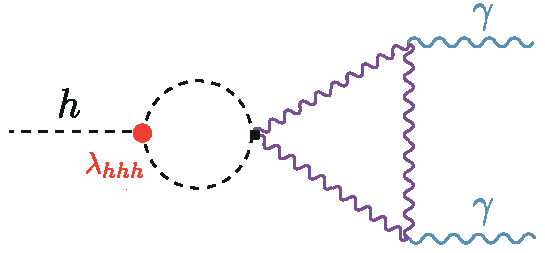
\includegraphics[width=0.8\textwidth]{figures/htoaa_nlo_ew}
		\caption{NLO EW corrections of single Higgs processes,  were the Higgs trilinear self-coupling~(the red circle) enters. Here the Higgs decay to two photons is shown as an example. \label{fig:h_nlo_ew} }
	\end{center}
\end{figure}
Using the results from the aforementioned references, a global fit with all operators that enter at tree-level in addition to the loop effects from the Higgs self-coupling has been preformed in refs.~\cite{DiVita:2017eyz,Dawson:2020oco}. Additionally, experimental searches for Higgs trilinear self-coupling have been presented by ATLAS~\cite{ATLAS:2019pbo} and CMS \cite{CMS:2020gsy}.\footnote{I present references here to the most recent results.} 
%%%%%%%
\subsection{Higgs pair production and SMEFT}
Higgs pair production in hadron colliders is sensitive to six~$\mathcal{CP}$ even SMEFT operators \footnote{For or Higgs pair production with~$\mathcal{CP}$ violating operators, see ref.~\cite{Grober:2017gut}. }, under the assumption of Minimal Flavour violation~(MFV).~\footnote{MFV assumes that new physics operators will follow the same flavour hierarchies as the SM.} These operators are
\begin{equation}
	\mathcal{O}_{\phi D},\ \mathcal{O}_{\phi \Box},\ \textcolor[HTML]{4334a0}{\mathcal{O}_{\phi}}, \ 	\textcolor[HTML]{2ebbaa}{\mathcal{O}_{t\phi}}, \ 	\textcolor[HTML]{ae0034}{\mathcal{O}_{\phi G}},\ \textcolor[HTML]{ffb743}{\mathcal{O}_{t G}},
	\label{HH-smeft}
\end{equation}
and their effects, with the corresponding colours are demonstrated in~\autoref{fig:hh-smeftw}, except for~$\mathcal{O}_{\phi D}$ and  $\mathcal{O}_{\phi \Box}$, as they modify all SM Higgs vertices. 
\begin{figure}[t!]
	\begin{center}
		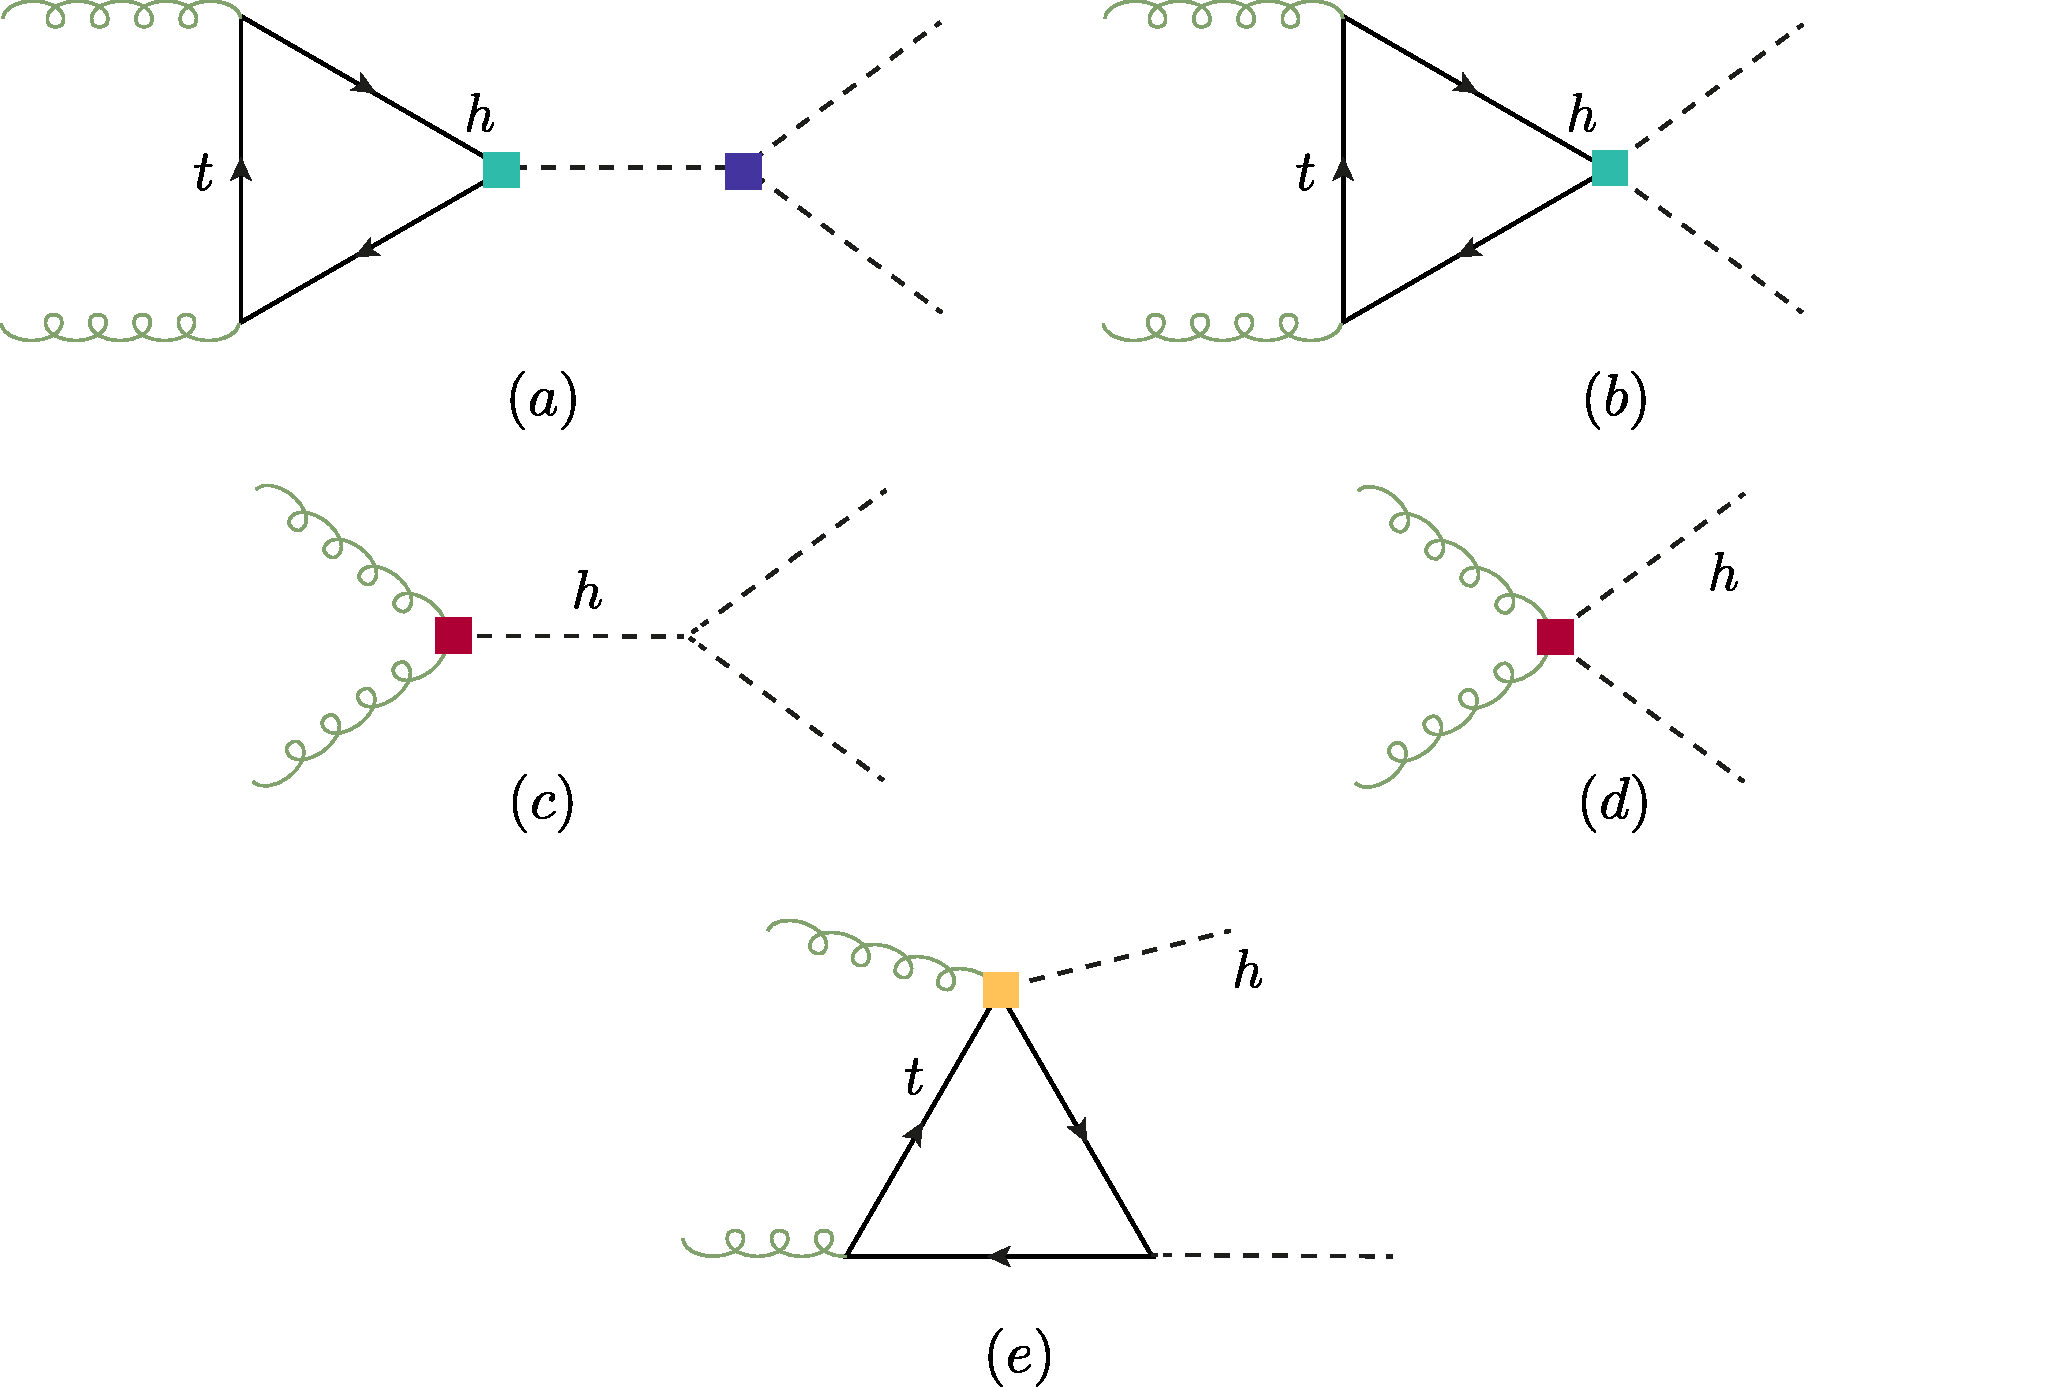
\includegraphics[width=0.75\textwidth]{figures/hh-smeft}
		\caption{ Example of diagrams illustrating how the dimension-six SMEFT operators enter in Higgs pair production at hadron colliders. \label{fig:hh-smeftw} }
	\end{center}
\end{figure}
However, MFV is not the only way to approach SMEFT, there exist more complex flavour structures that allow for significant enhancements of the first and second generation Yukawa couplings without being excluded by flavour observables. Such formalisms will be discussed in~\autoref{chap:lightyuk}.
The primary operator to constrain from Higgs pair as mentioned before is $\mathcal{O}_{\phi}$, for two reasons; a) the rest of the operators appearing in di-Higgs can be strongly constrained from single Higgs and top quark processes. b) The effect of $\mathcal{O}_{\phi}$ on Higgs pair production is significantly higher than in single Higgs or EW observables. This is illustrated in~\autoref{fig:hh-vs-h} by comparing the relative change of the gluon fusion cross-sections at NLO QCD for single and di-Higgs production. This is not surprising since $C_\phi$ appears at LO in Higgs pair production.
\begin{figure}[h!]
	\begin{center}
		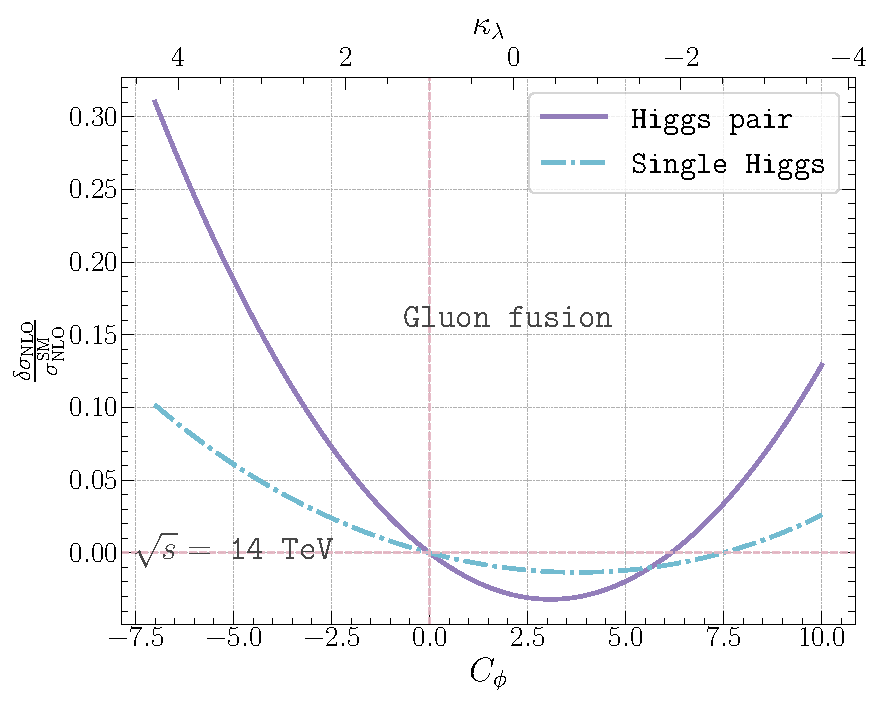
\includegraphics[width=0.65\textwidth]{figures/trilinear_single_vs_double}
		\caption{ The relative change of the NLO QCD cross-section of gluon fusion production of single Higgs (dashed line) and Higgs pair (solid line) at a $pp$ collider with $\sqrt{s}=14$ TeV as a function of $C_\phi$ or the corresponding $\kappa_\lambda$. \label{fig:hh-vs-h} }
	\end{center}
\end{figure}
Another advantage for Higgs pair production searches is the sensitivity of this process to non-linear couplings, for example, diagrams (b) and (d) of ~\autoref{fig:hh-smeftw}. Although in SMEFT, these diagrams correspond to the same operators in (a) and (c), respectively, in another EFT, this is not necessarily the case.
\section{The Higgs effective field theory\label{sec:chiral}}
Given the strong bonds on the $\rho$ parameter, it would be plausible to assume that the NP maintains the custodial symmetry~$SU(2)_V$ and treats the chiral symmetry breaking pattern $SU(2)_L \otimes SU(2)_R \to SU(2)_V$  the same way the QCD chiral symmetry breaking is treated. Considering the pions as pseudo-Nambu Goldstone bosons to describe their properties and couplings. In the pion case, this is known as \textbf{chiral perturbation theory}~\cite{GASSER1984142, GASSER1985465}. The same mathematical description could be applied to the case of EW symmetry breaking by constructing the EW chiral Lagrangian~(EWChL).   In this formalism, the Goldstone bosons~$\pi^a(x)$ of the SM are considered the generators of $SU(2)_L$ unitary transformation.
\begin{equation}
	\mathcal U(x) = e^{ i \pi^a(x)\sigma_a/v }, 
\end{equation}
which implies that the Goldstone fields transform non-linearly under~$SU(2)_L \otimes SU(2)_R$.  As for the Higgs boson~$h(x)$, it is added as an $SU(2)_L \otimes U(1)_Y$ singlet, and can appear in the EWChL at any power. Contrary to the SMEFT power counting in the NP scale $ \Lambda$, in the EWChL, terms are ordered according to their \emph{chiral dimension} $\chi$, defined for spacetime derivatives $\partial_\mu$,  bosonic $\phi, X_\mu$ and $\psi$ fermionic generic fields as~\cite{Buchalla:2013rka,Buchalla:2015wfa}
\begin{equation}
	[\phi]_\chi =0,\,\, [X]_\chi =0,\,\, [\partial_\mu ]_\chi =1, \,\, [\psi]_\chi =2.
\end{equation}
The zeroth-order term of the EWChL possesses a chiral dimension of $\chi=2$, while higher-order terms could be considered terms generated perturbatively from $L$ loop interactions, an having a chiral dimension~$\chi= 2L+2$. The expansion of the EWChL is in the chiral order in addition to the powers of $h(x)/v$. This power-counting causes some SMEFT dimension-six operators to be considered of a higher order in EWChL. A prominent example of this is the chromomagnetic operator~$\mathcal O_{tG}$ being of chiral dimension five. \\
The relevant terms for single- and di-Higgs production of the EWChL are given in the Unitary gauge by~\cite{LHCHiggsCrossSectionWorkingGroup:2016ypw,DiVita:2017eyz}
\begin{align}\nn
	\mathcal{L}_{\mathrm{HEFT}} = & \, \frac{h}{v} \Bigg[  \left( \delta c_W m_W^2 W_{\mu}^+W^{-\mu} +\delta c_Z \frac{m_Z^2}{2} Z_\mu Z^\mu\right)  \\\nn
	&+c_{ww}\frac{g_2^2}{2}W_{\mu\nu}^+W^{-\mu\nu} + c_{w\square} g_2^2\left(W_{\mu}^-\partial_\nu W^{+\mu\nu} + \text{h.c.}\right) +  c_{\gamma\gamma}\frac{\alpha}{8 \pi}A_{\mu\nu}A^{\mu\nu} \\\nn
	& +c_{zz}\frac{g_2^2 + g_1^2}{4} Z_{\mu\nu}Z^{\mu\nu}+ c_{z\gamma}\frac{e g_1}{16 \pi^2}Z_{\mu\nu}A^{\mu\nu}
	+c_{z\square}g_2^2Z_\mu\partial_\nu Z^{\mu\nu}
	+c_{\gamma \square}g_2 g_1 Z_\mu\partial_\nu A^{\mu\nu}
	\Bigg]\\\nn
	&+ \frac{\alpha_s}{8 \pi} \left( c_{gg} \frac{h}{v} +  c_{gg}^{(2)} \frac{h^2}{2 v^2}\right) \Tr[G_{\mu\nu} G^{\mu\nu}]
	-\sum_f \left[ m_f \left(c_f \frac{h}{v} + c _{ff} \frac{h^2}{2v^2}\right) \bar{f}_{R}f_{L}+\text{h.c.}\right]\\
	& - c_{hhh} \frac{m_h^2}{2 v} h^3\ + \dots,\label{eq:coupl_def}
\end{align}
I have omitted here the kinetic and mass terms of the Higgs, $\mathcal{CP}$ violating terms, as well as couplings not relearnt to LHC phenomenology and higher chiral order operators. \\
In addition to NP effects, this Lagrangian also includes the LO and NLO SM vertices, for example the parameter $\delta c_V=1$ corresponds to the tree-level coupling between the Higgs field and the EW bosons~$ V=W, Z$. While the coupling $c_{gg}= 4/3$ corresponds to the SM effective coupling at NLO if the heavy top limit~(HTL)~$m_t \to \infty$ is applied. \\
In contrast to the SMEFT, the couplings of one and two Higgs bosons to fermions or gluons become de-correlated. Giving this Lagrangian a richer phenomenology for Higgs pair production.  \\
The HEFT coefficients modifying the Higgs pair production via gluon fusion are 
\begin{equation}
	\textcolor[HTML]{4334a0}{c_{hhh} }, \ 	\textcolor[HTML]{2ebbaa}{c_t}\ (a) , \  	\textcolor[HTML]{2ebbaa}{c_{tt}} \ (b), \  \textcolor[HTML]{ae0034}{c_{gg}} \ (c), \  \textcolor[HTML]{ae0034}{c_{gg}^{(2)}} \ (d),
\end{equation}
with the same colours highlighted in the operator insertions of~\autoref{fig:hh-smeftw} and the letter next to the coefficient indicates the diagram, in which the coefficient appears.  Full parametrisation of the Higgs pair cross-section at NLO (inclusive and differential) and NNLO (inclusive) can be found in refs.~\cite{Buchalla:2018yce,Capozi:2019xsi,deFlorian:2021azd} and implemented at NLO in \texttt{POWHEG-BOX}~\cite{Heinrich:2020ckp}. \\ UV-complete models that are related to the EWChL are composite Higgs models~\cite{Contino:2010rs,Panico:2015jxa,AGASHE2005165}, dilaton theories~\cite{PhysRevLett.100.111802}, techni-dilaton models~\cite{Habaa:2010rbs}, technicolour models~\cite{Delgado:2010bb} and other models with induced EW symmetry breaking~\cite{Galloway:2013dma,Chang:2014ida}.
\subsection{Translation between SMEFT and HEFT }
In order to facilitate the translation between SMEFT and HEFT or to the $\kappa$-formalism, one needs to put the SMEFT Lagrangian into the canonical form, that is to convert the operators with covariant derivatives acting on the Higgs to canonically normalised Higgs kinetic term. This is done done by the field redefinition.
\begin{equation}
	\phi=\left( \begin{array}{c} 0 \\ h(1+c_{h,kin}) + v \end{array} \right),
\end{equation} 
with 
\begin{equation}
	c_{h,kin}=\left(C_{\phi,\Box}-\frac{1}{4}C_{\phi D}\right) \frac{v^2}{\Lambda^2}\,.
\end{equation}
This field redefinition will generate derivative interactions of the form $h(\partial_{\mu}h)^2$ and $h^2(\partial_{\mu}h)^2$. In order to remove these terms, and for sake of simplicity, I use a gauge-dependent field redefinition\footnote{For gauge-independent formalism cf.~ \cite{Hartmann:2015aia}.}
\begin{equation}
	h \to h + c_{h,kin}\left( h +\frac{h^2}{v}+\frac{h^3}{3v^2}\right)\,. \label{fieldref}
\end{equation}
This field redefinition leads to n $c_{h,kin}$ modifying all Higgs couplings. \\
Before discussing the translation between SMEFT and HEFT, some words of caution are in order: First, HEFT is less restrictive than SMEFT; therefore, it contains more degrees of freedom. This makes some points of the HEFT parameter space unmappable to SMEFT. In addition, the power counting is different in both formalisms, as mentioned before. Some operators present in SMEFT will be absent in HEFT and vice-versa.  In ~\autoref{tab:translation}, the translation between the HEFT and SMEFT Wilson coefficients of the operators relevant to Higgs pair production at LO is shown. 
\begin{table}[htb]
	\begin{center}
		\begin{tabular}{ c c }
			\toplinetwo
			HEFT& SMEFT (Warsaw)\\
			\midrule
			$c_{hhh}$&$1-2\frac{v^4}{m_h^2}C_\phi+3c_{h,kin}$ \\
			$c_f$ & $1+c_{h,kin} -C_{f\phi} \frac{v^3}{\sqrt{2} m_f}$\\
			$ c_{ff} $ &$-C_{f\phi} \frac{3 v^3}{2\sqrt{2} m_f} + c_{h,kin}$\\
			$c_{gg}$  & $8\pi/\alpha_s v^2 C_{\phi G}$ \\
			$c_{gg}^{(2)}$  & $4\pi/\alpha_s v^2 C_{\phi G}$ \\
			\bottomrule
		\end{tabular}
	\end{center}
	\caption{Translation between the Wilson coefficients of HEFT and SMEFT for the operators relevant to Higgs pair production. \label{tab:translation}}
\end{table}
More general translation between SMEFT in Warsaw and SILH basis and HEFT can be done automatically using \texttt{Rosetta} package~\cite{Falkowski:2015wza}
\subsection{EFT and $\kappa$-formalism \label{eftkappa}}
The $\kappa$-formalism provides an experimentally accessible and well-defined QFT-wise approach to study the Higgs boson properties. The $\kappa$ parameters are part of a more generalised formalism called the Higgs \textbf{Pseudo-observables}~\cite{Gonzalez-Alonso:2014eva}. 
If the new physics contributions do not generate new Lorentz structures, there is a possible translation between the Wilson coefficients in the SMEFT Warsaw basis and the $\kappa$ formalism. In particular, taking the rescaling of the trilinear coupling, $\kappa_\lambda$, the translation is given by
\begin{equation}
	\kappa_\lambda = 1-\frac{2v^4}{m_h^2} \frac{C_\phi}{\Lambda^2}+3 c_{h,kin}.
\end{equation}
A similar relation exists for the rescaling of the quark Yukawa couplings~$\kappa_q$
\begin{equation}
	\kappa_q = 1+c_{h,kin}- \frac{v^3}{\sqrt{2}m_q}\frac{C_{q\phi}}{\Lambda^2}.
\end{equation}
In these two examples, one can see the similarities between $\kappa$-formalism and HEFT, but this is not always the case.  Other translations could be obtained by comparing how SMEFT operators modify the Higgs couplings with the SM and matching it with the corresponding $\kappa$ or other Higgs pseudo-observable.\\ 
However, one should be careful while interpreting results quoted in terms of Wilson coefficients in the SMEFT framework extracted from multi-Higgs or multi-vector bosons searches. These results include couplings that are not present in the SM. For example, the $hh q\bar{q}$ coupling, though being linearly related to the quark Yukawa coupling $h q\bar{q}$, is not a rescaling of any SM Higgs coupling. With this in mind, one can strictly remain within a linear EFT and link the rescaling of the quark Yukawa, $\kappa_q$, to the~$hh q\bar{q}$ coupling through
\begin{equation}
	g_{hhq\bar{q}}^{\mathrm{linear-EFT}} = -\frac{3}{2}\frac{1-\kappa_q}{v} \, g_{h q\bar{q}}^{\mathrm{SM}}.
\end{equation}
This relation will no longer hold once a non-linear EFT, like HEFT, is used. Hence, the $\kappa$-formalism must be applied carefully when multi-Higgs signals are considered.
\section{Conclusions \label{sec:concefts}}
Effective field theories provide a systematic yet simplified approach for NP searches by simplifying its complex interaction structures. This can be viewed as a dimensionality reduction approach and collapsing all the NP interactions into effective ones. They would be observed at colliders with energy reaches below the NP scale $\Lambda$. The linear approach to EFT is called the SMEFT that preserves the SM fields and symmetries, and the Higgs boson is a part of an $SU(2)_L$ doublet $\phi$ like the SM. In contrast, non-linear approaches such as HEFT/EWChL treat the Higgs boson as an added singlet. The latter approach is more general and introduces independent parameters involving multiple Higgs bosons. For example, the couplings $f\bar f h$ and $ f\bar f hh$ will be generated in SMEFT and HEFT. Still, in SMEFT, both are related by the Wilson coefficient $C_{\phi f}$, while in HEFT, they have independent  Wilson coefficients $c_f$ and $c_{ff}$, respectively. \\  Most of the Wilson coefficients involving Higgs interactions are strongly constrained by EWPOs and Higgs and top-quark data. However, the bounds on the Wilson coefficient modifying Higgs self-couplings $C_\phi$ remain dominated by theoretical constraints from perturbative unitarity~\cite{DiLuzio:2017tfn,DiVita:2017vrr}. This can be improved by the searches for Higgs pair production at the HL-LHC, as this process is more sensitive to the trilinear Higgs self-coupling than EWPO and single-Higgs data.
%\begin{figure}[htbp!]
%	\begin{center}
	%		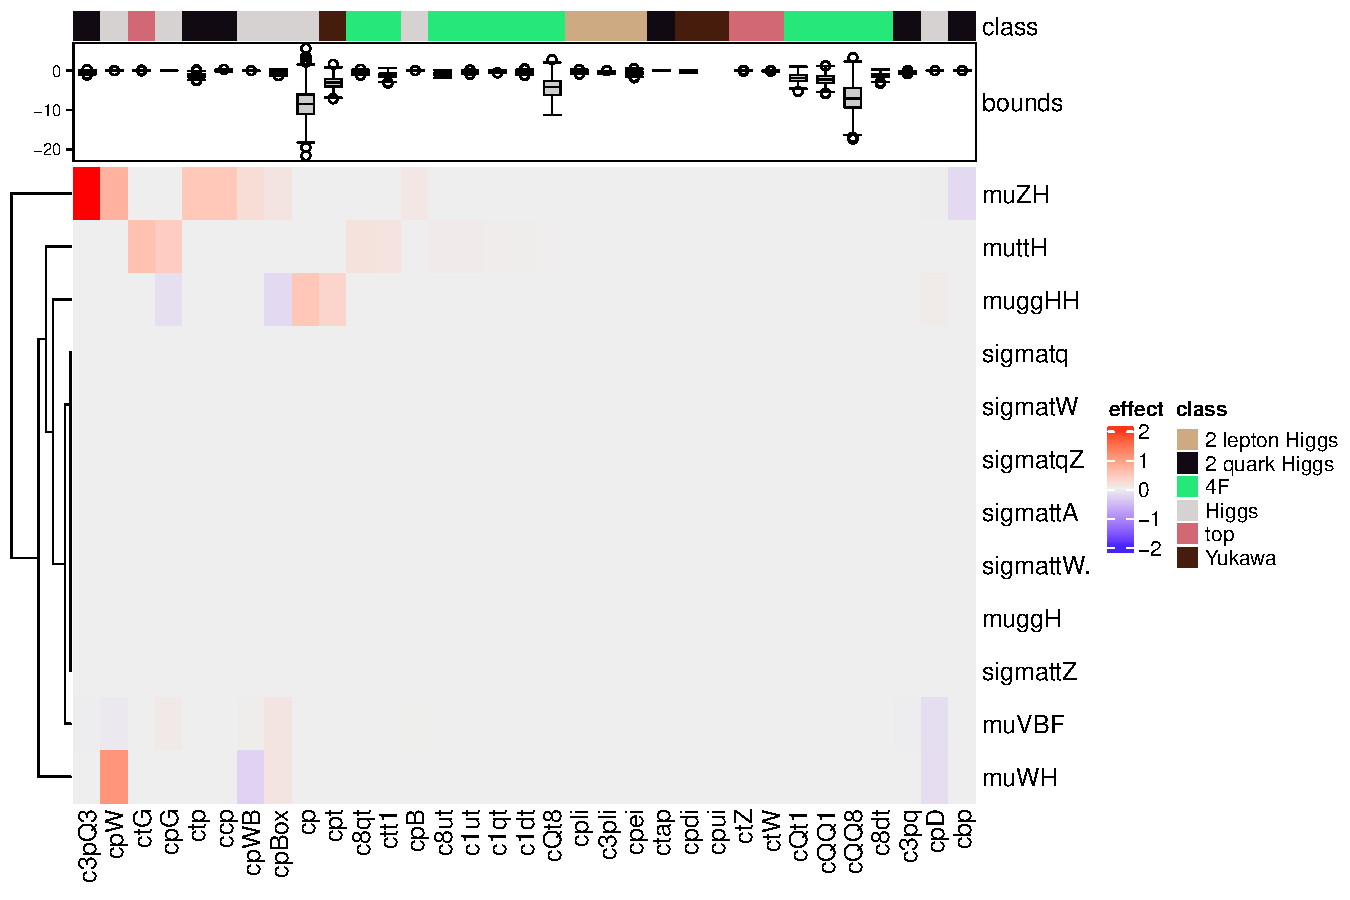
\includegraphics[width=\textwidth]{figures/smeft_heatmap}
	%		\caption{ \label{fig:greatheatmap} }
	%	\end{center}
%\end{figure}
%In~\autoref{greatheatmap}, I show the best bounds on the Wilson coefficients relearnt to Higgs production as well as heavy quark four-fermion operators, with a heatmap indicating the contribution of each operator in prominent Higgs, top and EW precision observables.  Although this is a subset of the total SMEFT operators and observables used in the fits, one can see the interconnectivity of the measurements.\\ The main objective of this thesis is to extend these connections by exploiting the potential of single-Higgs data and Higgs pair production to constrain the Higgs trilinear coupling modifiers (mainly in SMEFT) and the interplay between $C_\phi$ and heavy quark four-fermion operators in single Higgs data. Moreover, the SMEFT picture can be further extended by unravelling the interplay between Light quark couplings modifiers in Higgs pair production. Lastly, I will show another connection between Higgs operators in SMEFT and flavour anomalies.  Emphasising the complex interconnectivity between experimental observables and SMEFT operators. 
%%%%%%%
       
        % Part 2

        \part{Single Higgs Processes at the LHC }
        %!TEX encoding = UTF-8 Unicode
% !TeX spellcheck = en_GB

%%%%%%%%%%%%%%%%%%%%%%%%%%%%%%%%%%%%%%
\chapter{ Overview of Higgs production at colliders }\label{chap:overviewSingleHiggs}
%%%%%%%%%%%%%%%%%%%%%%%%%%%%%%%%%%%%%%
Four distinct processes mediate the production of the Higgs boson at the LHC: gluon fusion~(ggF), vector-boson fusion~(VBF), vector bosons Higgsstrahlung~($Vh$), and the production with top ( and anti-top) pair~($th / t \bar th$). It should be noted that sometimes the ggF category will include the quark anti-quark annihilation, but this is negligible in the SM but becomes important for significant modifications of light Yukawa couplings. These processes are illustrated in~\autoref{fig:singlehiggs}, and their details were summarised in~\autoref{table:singlehiggs}. These four channels have been observed at the LHC with $>5 \sigma$ precision. \\ 
Since the experimental measurements of this Higgs were discussed previously in~\autoref{sec: Higgscoupl}, this chapter aims to provide an overview of the current theoretical status of these channels.
\begin{table}[htbp!]
	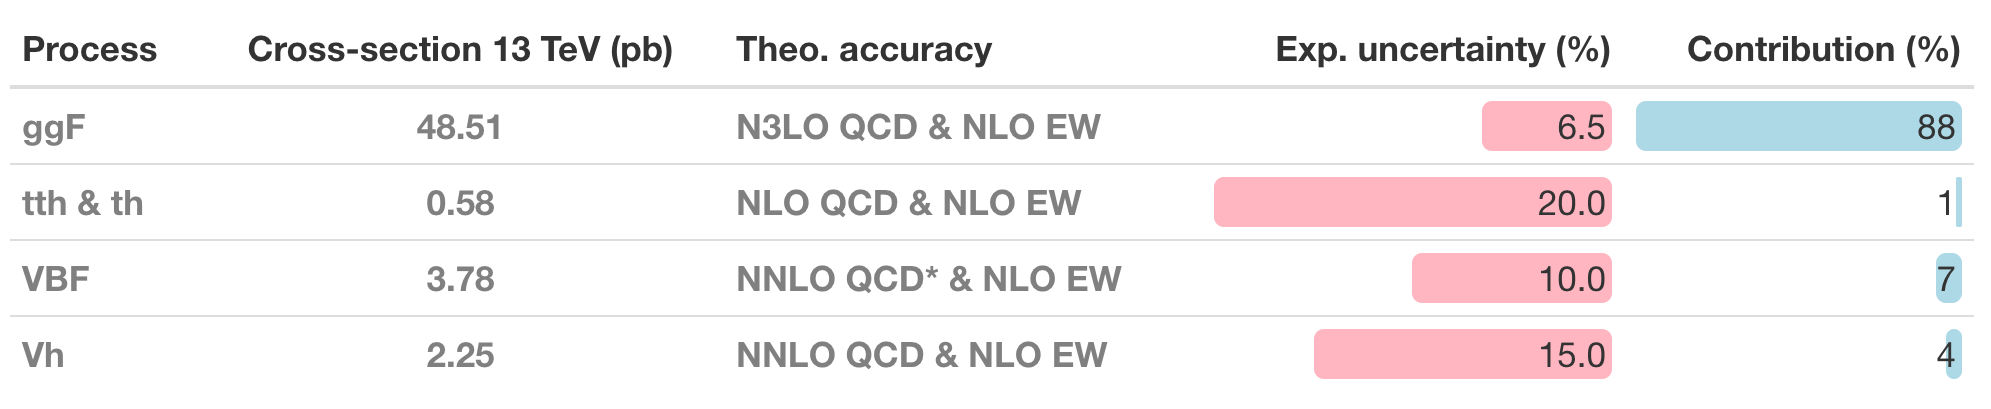
\includegraphics[width=1\textwidth]{single_higgs_table}
	\caption{ Summary  of the Higgs production processes at the LHC. \label{table:singlehiggs} }
\end{table}
\begin{figure}[htbp!]
	\begin{center}
		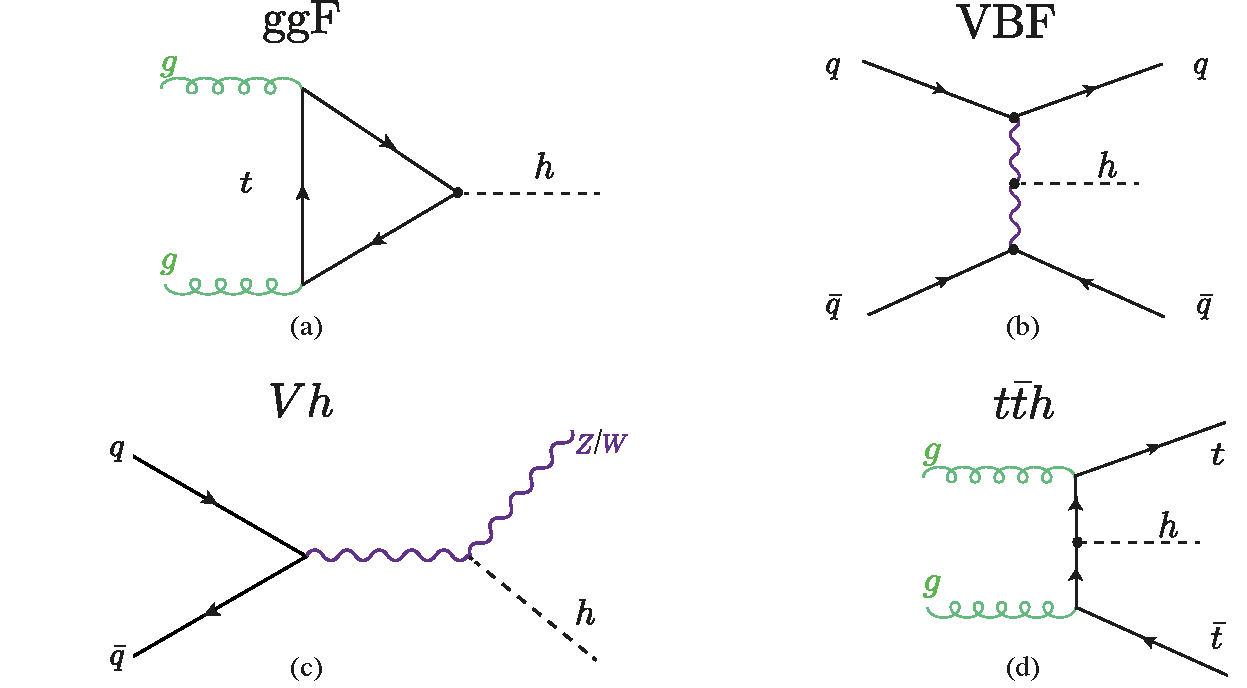
\includegraphics[width=.75\textwidth]{figures/single_higgs}
		\caption{Feynman-diagram examples of the leading  Higgs production processes  at the LHC. \label{fig:singlehiggs} }
	\end{center}
\end{figure}
\section{Current status of the Higgs production channels  \label{sec:singlehiggschannels}  }
\subsection{Gluon fusion process}
The Higgs production via gluon fusion~(ggf)  has the highest cross-section amongst the Higgs production channels, and consequently has the lowest experimental uncertainty. The current state-of-the-art theoretical computation for the Higgs inclusive cross-section is N$\,^3$LO in QCD and NLO in EW~\cite{Bonetti:2018ukf}. A full differential cross-section for the final state $ gg \to h \to \gamma \gamma$ has been computed recently to~N$\,^3$LO in QCD, also for the kinematic variables~$y_h, \ y_{\gamma_1},\ y_{\gamma_2},\ \Delta y_{1,2}$ using the projection-to-born method~\cite{Chen:2021isd}.In addition to the fiducial differential cross-section in $\pt$ with experimental cuts has been computed up to third re-summed and fixed order, i.e.  N$\,^3$LL$^\prime$   N$\,^3$LO dependence~\cite{Billis:2021ecs}. The theoretical computation of this fiducial cross-section with different orders compared to the experimental measurement by ATLAS~\cite{ATLAS:2019jst} is shown in~\autoref{fig:ggFxs}, we can see that the resummed result has significantly smaller theoretical uncertainties. The current total theoretical uncertainty with this order calculation is $5.4 \%$, with only $2.7\%$ of it coming from the perturbation order cut-off of the calculation, while the rest comes from the branching fraction, PDF+$\alpha_s$, EW corrections and mass uncertainties. When compared to~\autoref{table:resHiggsExp}, the projected experimental uncertainty of this final states at the HL-LHC is $4.2\%$, we see that the uncertainties will become comparable, and if the PDF uncertainties are reduced.
\begin{figure}[htbp!]
	\begin{center}
		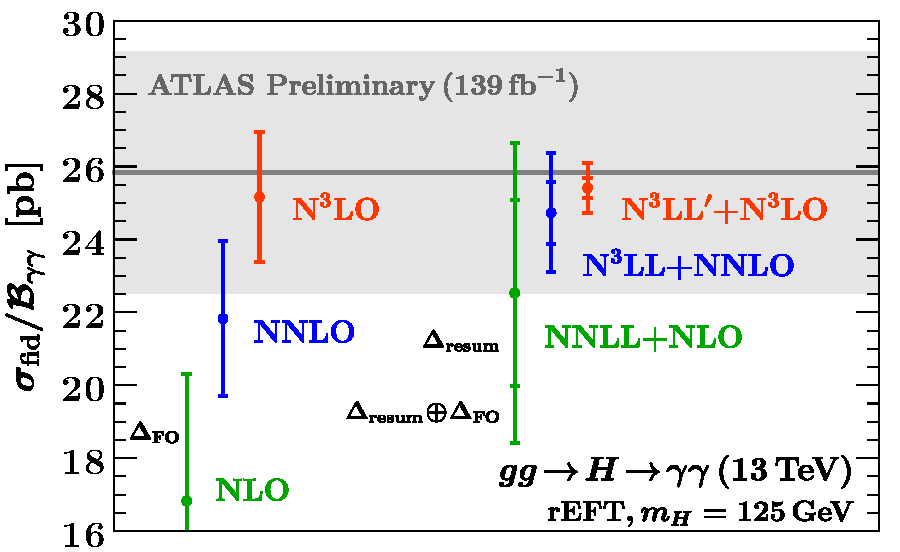
\includegraphics[width=.7\textwidth]{figures/total_xs_fid}
		\caption{ The total fiducial cross-section for the final state  $ gg \to h \to \gamma \gamma$ at both fixed and resumed third order compared to the experimental ATLAS measurement~\cite{ATLAS:2019jst} this figure is taken from~\cite{Billis:2021ecs}. \label{fig:ggFxs} }
	\end{center}
\end{figure}
The predictions can be further improved by the computation of mixed QCD-EW effects. These computations invokes three-loop integrals with both gluons and EW bosons, computed in~\cite{Bonetti:2017ovy} or two-loop ones with two particle final states appearing in the real corrections with the process $ gg \to hg$ computed in~\cite{Bonetti:2020hqh} using differential equations. The computation was completed by inclusion of light quark initial states for the real corrections in~\cite{Becchetti:2020wof} with exact quark mass dependence, reducing the EW uncertainty from $2\%$ to $ \sim 0.6\%$.  \\ The computation of the three-loop form-factors with full top-mass dependence  were carried out by~\cite{Czakon:2020vql,Czakon:2021yub}. However, there remains an intricate interplay between the mass effects of $gg$, $qg$ and $qq$ initial states for the real matrix elements that cannot be fully controlled due to the light quark mass effects. \\ NLO corrections to the $h +j$ and $ h+2j$ processes were computed by~\cite{Maltoni:2014eza} in the FT approximation, which used exact born and real correction amplitudes, and approximates the two-loop virtuals by
\begin{equation}
	|	\mathcal A^{\mathrm{2-loop}}(m_t,\mu_R^2) |^2 \approx  |	\mathcal A^{\mathrm{1-loop}}(m_t\to \infty,\mu_R^2) |^2\, \frac{|	\mathcal A^{\mathrm{1-loop}}(m_t) |^2}{A^{\mathrm{(0)}}(m_t)\to \infty |^2}. 
\end{equation}
This approximation works superbly even for $ \pt \gg m_t$. Later, the full top mass effects computations have been carried out in~\cite{Kudashkin:2017skd, Lindert:2018iug, PhysRevLett.120.162001} using the high energy~(HE) expiation technique. 
\subsection{Vector boson fusion}
The VBF channel has a distinctive signature, making it a bona fide channel for Higgs signal extraction. The suppressed colour exchange between the quarks results in a little jet activity in the central rapidity region. The quarks will be scattered into two forward jets such that the decay products of the Higgs are found in the region between them.  These features allow for excellent measurement of Higgs couplings, observation of challenging decays, and $\mathcal{CP}$ properties determination. Some of these features are also shared with the $Vh$ production channel. Both of these channels contain the $VVh$ vertex, which could be written generally as~\cite{LHCHiggsCrossSectionWorkingGroup:2016ypw}
\begin{equation}
	T^{\mu \nu}(p_1,p_2) = a_1 g^{\mu \nu}+ a_2  \left(g^{\mu \nu}- 2\frac{p^\mu_{2} p^\nu }{p_1 \cdot p_2} \right)  + a_3 \frac{p_1^\alpha p_2^ \beta}{p_1 \cdot p_2}\epsilon^{\mu \nu \alpha \beta}. 
\end{equation} 
In the SM, only $a_1\neq0$, while the rest of the coefficients represent the anomalous coupling. For example, if $a_3 \neq0$, then the Higgs is  $\mathcal{CP}$  odd. The study of the azimuthal angle distribution~$d \sigma_{VBF} / d \Delta \phi_{jj}$ allows for the determination of these coefficients, with very little dependence on the Higher-order corrections~\cite{hankele2006anomalous}.\\  The NLO QCD inclusive cross-section is known since the 90's~\cite{Han:1992hr}, and later these corrections were made for the differential distributions cf.~\cite{Figy:2003nv,Berger:2004pca}. Unlike the ggF channel, which has an NLO  K-factor of $1.6$ at 13 TeV~\cite{Gomez-Bock:2007azi}, the VBF NLO corrections are small $\sim 10\%$. The two-loop NNLO QCD cross-section has also been computed, and the most recent results of the two-loop computation were calculated via the structure-function approach~\cite{Bolzoni:2010xr} in addition to STXS level 1.2 bins with EW corrections~\cite{Denner:2014cla}. These calculation are implemented in the MC event generator  \texttt{HAWK}. Despite these small corrections, they are non-negligible, and their inclusion is important for uncertainty reduction.
\subsection{Associated production with EW bosons \label{vhproduction}}
The vecctor boson Higgsstrahlung channels $pp\to Wh/Zh$ at LO are quark-initiated tree-level processes  interpreted as \textbf{Drell-Yan process}~ \cite{Han:1991ia,Brein:2003wg}. They have been computed up to  NNLO in QCD ($\sim \alpha_s^2$), and  NLO  EW  ($\sim \alpha^2 $)~\cite{Amoroso:2020lgh}.
%%
\par Despite arising for the first time at NLO, the gluon fusion channel $g g \rightarrow Zh$ has a non-negligible contribution to the total hadronic cross-section~$pp\to Zh$, which could reach $>16\%$ of the total cross-section contribution at $14$ TeV~\cite{Cepeda:2019klc}, see~\autoref{fig:hzratio}. The contribution becomes more significant when looking at large invariant mass bins of the differential cross-section. This is due to the substantial abundance of gluonic PDFs at the LHC and the extra enhancement coming from the top quark initiated contribution near the~$t\bar t$ threshold to boot~\cite{Englert:2013vua}. Still, also it has a higher scale uncertainty than the quark anti-quark annihilation~$\qqA$ channel.  With these points in mind, and the absence of a gluon fusion channel for the $Wh$ channel, the $Zh$ channel has higher theoretical uncertainties than~$Wh$. This motivates the need to calculate the  $g g \rightarrow Z h$ channel to higher orders in perturbation theory to reduce these uncertainties. The inclusion of the two-loop calculations for the ggF part would facilitate the precision measurement of the $Zh$ channel at the future LHC runs, which in terms provides better constraints on several observables, such as sign and magnitude of the top Yukawa and $ZZh$ couplings amongst others~\cite{Englert:2016hvy}.
%%
\begin{figure}
	\begin{center}
		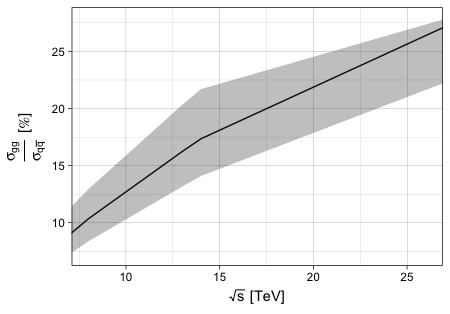
\includegraphics[width=9cm]{./figures/Rplot}
		\caption{The ratio of the LO gluon fusion production cross-section $ gg \to Zh$  ($\sigma_{gg}$) with respect to the NLO Drell-Yan process $ q\bar{q} \to Zh$ cross-section ($\sigma_{q\bar{q}}$) at a $pp$ collider with centre-of-mass energy $\sqrt{s}$. The error band captures the total theoretical uncertainties on both cross-sections dominated by~$\sigma_{gg}$ .}
		\label{fig:hzratio}
	\end{center}
\end{figure}
%%
\par  The leading order (LO) contribution to the $g g \rightarrow Z h$ amplitude, given by one-loop diagrams, was computed exactly in refs.\cite{Kniehl:1990iva, Dicus:1988yh}. For the NLO computations, the virtual corrections contain multi-scale two-loop integrals, some of which are still not known analytically, making these computations a formidable task. The first computation of the NLO terms has been done by~\cite{Altenkamp:2012sx}, where the HTL asymptotic expansion and setting $m_b = 0$. The HTL NLO computations pointed to a significant $K$-factor of about $\sim2$.  Later, the computation has been improved via soft gluon resummation, including NLL terms found in ref.\cite{Harlander:2014wda}. The NLL matching the fixed-order NLO computation can be found in ref.~\cite{Altenkamp:2012sx}.  Top quark mass effects were first implemented using a combination of  HTL  and Pad\'e approximants~\cite{Hasselhuhn:2016rqt}. A data-driven approach to extract the gluon fusion dominated non-Drell-Yan part of $Zh$ production using the known relation between  $Wh$
and $ Z h$ associated production when only the Drell-Yan component of the two processes is considered has been investigated in ref.\cite{Harlander:2018yns}. The differential distributions of $g g \rightarrow Zh$  at NLO were studied in ref.\cite{Hespel:2015zea} via LO matrix element matching. 
%%
\par More recent studies of the NLO virtual corrections to this process were based on the high-energy~(HE) expansion improved by Pad\'e approximants with the LME, which extended the validity range of the HE expansion \cite{Davies:2020drs}. However, this expansion is only valid for in the invariant mass region $\sqrt{\hat{s}}  \gtrsim 750\, \si{\GeV} $ and $\sqrt{\hat{s}}  \lesssim 350\,  \si{\GeV}$,  which only covers $\sim 32\%$ of the hadronic cross-section. Additionally, numerical computation of the two-loop virtual corrections, though implemented exactly in  \cite{Chen:2020gae}, are rather slow for practical use in MC simulations.  This highlights the importance of an analytical method that can cover the remaining region of the cross-section and can be merged with the HE expansion via Pad\'e approximants. Fortunately, the two-loop corrections to the triangle diagrams can be computed exactly. And the loop integrals appearing in the box correction having no analytic expression can be expanded in small  $Z$ (or Higgs) 
transverse momentum, $\pt$. This method was first used for Higgs pair production in~\cite{Bonciani:2018omm} to compute the NLO virtual corrections to the box diagrams in the forward kinematics. In~\autoref{chap:hz}, I will discuss the calculation performed by my collaborators and myself and published in~\cite{Alasfar:2021ppe}, which includes the full top mass dependence of the virtual two-loop correction to~$ gg \to Zh$ in an analytic form using the same $\pt$ expansion technique.

\subsection{Associated production with top quarks}
The largest part of the $t\bar t h/th$ uncertainty budget comes from the theoretical modelling of this process's backgrounds, mainly $t \bar t b\bar b,\ t\bar t W$ as backgrounds for $ t\bar t (h \to b\bar b)$ and $ t \bar t ( h \to \mathrm{multileptons})$, respectively. There have been several theoretical developments regarding these backgrounds. Starting with $t\bar t W$, the differential cross-section at NNL+ NLO QCD calculation of this channel has been done in~\cite{Broggio:2019ewu,Kulesza:2020nfh} including EW corrections. The fully decayed final state at NLO QCD~\cite{Bevilacqua:2020pzy,Denner:2020hgg,Bevilacqua:2020srb} and at NLO-EW~\cite{Denner:2021hqi} have been computed. Additionally, these calculations were implemented in~\texttt{POWHEG-BOX}~\cite{Cordero:2021iau}. The comparison between the NLO-QCD with Parton showering vs on-shell can be found in~\cite{Bevilacqua:2021tzp}. As for ~$t \bar t b\bar b$, the progress in obtaining higher-order corrections is faced with challenges posed by the complexity of this channel. However, progress has been made; for instance, the off-shell effects in the fully decayed $ pp \to 2 \ell 2 \nu  4 b$ with NLO corrections were studied in~\cite{Denner:2020orv, Bevilacqua:2021cit}. Further discussion of the theoretical developments of these channels is beyond the scope of this thesis. \\
Regarding the higher-order corrections to the $t\bar t h /t h$ channel itself, the NLO QCD+EW effects on the off-shell multileptons final state were studied in~\cite{Denner:2019zdz}. In contrast, the NLO corrections, including SMEFT operators, were calculated in\cite{Maltoni:2016yxb}. The NLO QCD+EW with Parton showering is available in all event generators, and the SMEFT operators at NLO are available in \texttt{MadGraph5\_aMC@NLO}.  As of writing this thesis, there is no NNLO calculation of $t\bar t h /t h$ available. 
%\section{Higgs pseudo-observables \label{sec:higgspos}  }

\section{Concluding remarks \label{sec:singlehiggsconc}  }
The precision-era of Higgs measurements requires developments on both experimental and theoretical levels. The experimental precision can be improved with Higher luminosities and energies, better detectors and improved analysis techniques. Theoretical uncertainties require higher-order calculations, the inclusion of mixed EW and QCD terms, the inclusion of mass effects and suitable Parton distribution functions with Higher order in QCD.  Much effort is being put into improving the theoretical predictions of Higgs production channels. Moreover, a plethora of computer tools have been made available to facilitate the computation of these cross-sections, for example  \texttt{iHixs2}~\cite{Dulat:2018rbf} or to generate full events, like \texttt{POWHEG}~\cite{Alioli:2008tz,Nason:2009ai,Bagnaschi:2011tu,Campbell:2012am,Luisoni:2013cuh,Jager:2014vna,Hartanto:2015uka} and \texttt{MadGraph5\_aMC@NLO}~\cite{Alwall:2014hca}, and many others can be found with greater detail in the LHC-HXWG Twiki page\cite{HXSWG}.  \\ Sometimes, to improve the measurement of the process, it is not sufficient to include Higher-order terms of the channel itself and its backgrounds, which is particularly important for $t\bar th $. Hence, higher-order calculations of processes like $t\bar t W$ with Parton-shower effects as well as improved analysis to distinguish $t\bar t(h \to b \bar b) $ have a significant impact on  $t\bar th $ measurements.
Event generator tools with SMEFT implementation for Higgs processes with patron showing interface capabilities have been implemented in a \texttt{MadGraph5\_aMC@NLO} model~\texttt{SMEFTatNLO}~\cite{Degrande:2020evl} which enabled loop computations with SMEFT operators and consequently fits of the SMEFT Wilson coefficients with Higgs data at NLO as we have seen in~\autoref{chap:HiggsEFT}.\\
There is plenty of room for future improvements in the reduction of theory uncertainty budget and providing better theoretical prediction of the Higgs processes in the SM and beyond, from the inclusion of patron shower matching, merging and validation to the inclusion of two-loop calculations of gluon fusion $Zh$  and EW NLO effects of  $t\bar the $, all in preparation for the HL-LHC Higgs precision era! 

%%%
%\begin{figure}
%	\begin{center}
	%		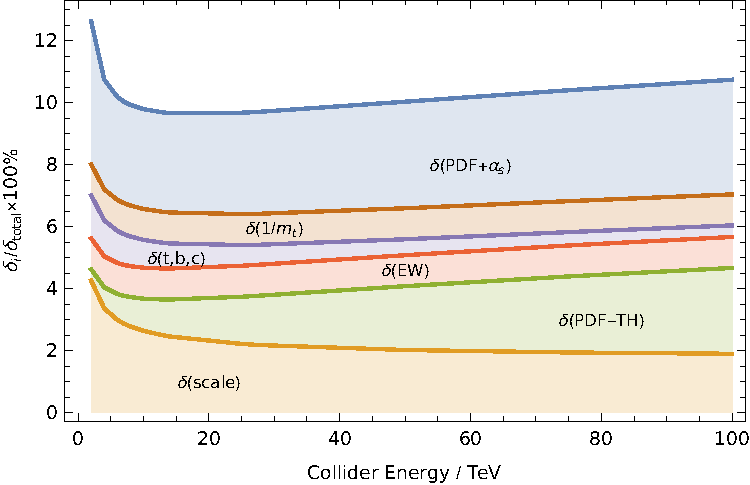
\includegraphics[width=9cm]{./figures/error_plot}
	%		\caption{The error budget plot showing the cumulative uncertainty of the total Higgs cross-section via gluon fusion at ~N$\,^3$LO as a function of energy. This plot is taken from~\cite{Dulat:2018rbf}}
	%		\label{fig:error-budget}
	%	\end{center}
%\end{figure}
%%%


%
%\subsubsection{The LO amplitude}
%We recall the projected LO on shell amplitude~\cite{Gunion:1989we}
%\begin{equation}
%	\mathcal{M}_{LO} = \frac{ T_f \alpha_s \ght }{2 \sqrt{2} \pi } \mathcal F^{(1 \ell)}  S_\epsilon ,
%\end{equation}
%with the projector
%\begin{equation}
%	\mathbb{P}^{\mu \nu} = g^{\mu \nu}- 2\frac{p^\mu_{2} p^\nu }{m_h^2},
%\end{equation}
%and the 1 loop form factor
%\begin{align}
%	\mathcal F^{(1 \ell)} &= m_h\,\sqrt{\tau} \left( (1-\tau) H(0,0,x)+2\right) ,\nonumber  \\
%	x &= \frac{\tau+2 \sqrt{1-\tau}-2}{\tau},
%	\label{f1l}
%\end{align}
%where $ \tau = 4 m_t^2/m_h^2$,  $H(m,n,x)$ is the harmonic ploylogarithm function~(HPL), and
%\begin{equation}
%	S_\epsilon = \Gamma(1+\epsilon) (\mu/m_t)^{2\epsilon}.
%\end{equation}
%\\
%The decay width is therefore given by
%\begin{equation}
%	\Gamma_{LO}(h\to gg) = \frac{\alpha_s^2\, G_F\,m_h^3 \,m_t^2\,\tau }{8 \pi^3 \sqrt{2}}  \, \left( 3(\tau-1)^2 H(0,0,0,0,x)+2(\tau-1)H(0,0,x)+2\right)
%\end{equation}
%With the following definitions
%\begin{align}
%	\ght &=\ght^{SM} = {\sqrt{2} m_t \over v}, \nonumber \\
%	v &= \left( G_F \sqrt{2}\right) ^{-1/2}, \nonumber \\
%	T_f &= \frac{1}{2} .
%\end{align}
         %!TEX encoding = UTF-8 Unicode
% !TeX spellcheck = en_GB


%%%%%%%%%%%%%%%%%%%%%%%%%%%%%%%%%%%%%%
\chapter{ Four top operator in Higgs production and decay}\label{chap:4topSingleHiggs}
%%%%%%%%%%%%%%%%%%%%%%%%%%%%%%%%%%%%%%


%The precise determination of the Higgs boson properties is one of the main focus of the Large Hadron Collider (LHC) physics programme. Within the current experimental precision, the measurement of the Higgs couplings so far appear to be in agreement with the Standard Model (SM) prediction within an accuracy of, typically, ten percent \cite{Aad:2019mbh, Sirunyan:2018koj}. In many beyond the SM (BSM) scenarios, however, it is expected that new physics will introduce modifications in the Higgs properties. 
%
%If the new BSM degrees of freedom are much heavier than the electroweak scale, a general description of potential new physics effects can be formulated in the language of an effective field theory (EFT). One possibility of such a parameterization is the so-called Standard Model EFT (SMEFT), in which new physics effects are given in terms of higher-dimensional operators involving only SM fields and that also respect the SM gauge symmetries.  The dominant effects on Higgs physics, electroweak physics and top quark physics stem from dimension-six operators, suppressed by the new physics scale $\Lambda$. This approach is justified in the limit 
%in which energy scales $E\ll \Lambda$ are probed. 
\par In the previous chapters, the SMEFT has been portrayed as  a robust and practical parametrisation of NP degrees of freedom for LHC searches, keeping in mind that these degrees of freedom have masses that are higher than the LHC reach. We have seen in~\autoref{chap:HiggsEFT} the SMEFT parametrisation for dimension-six operators involving the Higgs boson, and discussed some constraints on them. The operator~$ \mathcal O _{\phi}$ stands out as one of the weakly constrained SMEFT operators involving the Higgs, this is due to the current low experimental sensitivity on the Higgs self-coupling as shown in~\autoref{fig:higgs_kappa}. In order to probe the Higgs trilinear sel-coupling directly, one ought to observe Higgs pair production, see~\autoref{part:hh}. However, it has been proposed that bounds on the Higgs trilinear coupling could still be constructed from single Higgs data, and yield competitive constraints on this coupling than the current Higgs pair searches~ \cite{McCullough:2013rea, Gorbahn:2016uoy, Degrassi:2016wml, Bizon:2016wgr, Maltoni:2017ims, Degrassi:2019yix, Degrassi:2021uik, Haisch:2021hvy}, this due the appearance of the Hggs self-coupling in the NLO EW corrections to single Higgs processes, 
as~\autoref{fig:h_nlo_ew} demonstrates an example of such corrections.
\begin{figure}[htpb!]
	\begin{center}
		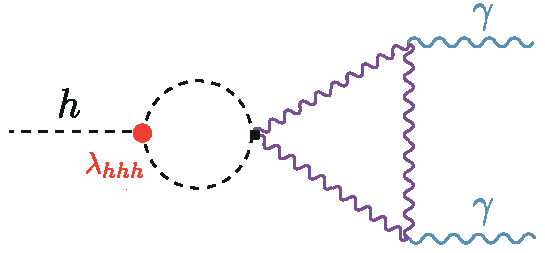
\includegraphics[width=0.45\textwidth]{figures/htoaa_nlo_ew}
		\caption{NLO EW corrections of single Higgs processes,  were the Higgs trilinear self-coupling~(the red circle) enters. Here the Higgs decay to two photons is shown as an example. \label{fig:h_nlo_ew} }
	\end{center}
\end{figure}
Using the results from the aforementioned references, a global fit with all operators that enter at tree-level in addition to the loop effects from the Higgs self-coupling has been preformed in ref.~ \cite{DiVita:2017eyz}. Additionally, experimental searches for Higgs trilinear self-coupling have been presented by ATLAS~\cite{ATLAS:2019pbo} and CMS \cite{CMS:2020gsy}.  
%%%%%%%
%Using the example of the four-quark operators, we will show that there are other weakly constrained dimension-six  operators, that enter at the loop level, that should be included in such analyses as they have a non-trivial interplay with the trilinear Higgs self-coupling extraction from single Higgs measurements. We will hence perform a combined fit of these operators together with the operator modifying the trilinear Higgs self-coupling. While our study does not consider a global fit to all operators entering Higgs data, the results of our computations can be easily used in global analyses. Our main point, namely that in a global fit all operators entering via loop contributions, if so far constrained only weakly (as it is the case for, e.g., four-top operators), should be included, is clearly demonstrated by our few parameters fit. 
%%%
\par The physics of the top quark and the Higgs are deeply intertwined, and when one starts looking at the operators entering at NLO of Higgs processes,  and by restricting oneself to pure Higgs or EW operators, one would miss the full picture in a global fit. Namely, the top quark operators. Though many of the top quark operators are strongly constraint from top observables, a few set of dimension-six operators remain as weakly constraint as the trilinear Higgs self-coupling or more. These operators are four-fermion operators involving the top quark. They would be constrained directly from the production of four tops observation. However, this process has a small cross-section at the LHC of $12\, \femtobarn$~\cite{Frederix:2017wme}, which is more or less comparable to the Higgs pair production. Experimental searches for the production of four top quarks has been first made byCMS~\cite{Sirunyan:2019nxl} combining different LHC runs, followed by ATLAS~\cite{Aad:2020klt}, the latter reporting a $4.3 \sigma$ observation of this processes with cross-section of $24^{+7}_{-6}\,\femtobarn$. When the whole third generation quarks is included, one sees the same story with~$t\bar{t}b\bar{b}$  contact interaction which require the observation of $t\bar{t}b\bar{b}$ production for a direct constraint, see \cite{Sirunyan:2020kgar, ATLAS:2018gug} for experimental searches and \cite{DHondt:2018cww, for Hartland:2019bjb} for SMEFT fits. It should be noted that for the production of four tops, or two tops two beauty quarks in SMEFT, the contact terms do not interfere with the SM process, and only appear proportional to $\mathcal{O}(1/\Lambda^4)$. This makes the SMEFT global analysis of these operators depend highly on the ETF truncation scheme used, i.e. whether to keep quadratic terms or not. 
\par
Given the rather weak ``direct'' bounds on the $t\bar{t}t\bar{t}$ and $t\bar{t}b\bar{b}$ contact interactions, here we will discuss alternative probes, showing how these interactions can be constrained indirectly via their contributions to single Higgs observables.\footnote{Alternatively, other indirect probes of four-top quark interactions that have been proposed include top quark pair production \cite{Degrande:2020evl} and electroweak precision data \cite{deBlas:2015aea}. The latter mostly leads to bounds on operators that can be constrained only weakly from Higgs data.}
These operators generate contributions to the effective couplings of the Higgs to gluons and photons via two-loop diagrams. At the one-loop level, they also modify associated production of a Higgs boson with top quarks and, in the case of a $t\bar{t}b\bar{b}$ operator, also the Higgs decay to bottom quarks. While the leading log results can be easily included by renormalisation group operator mixing effects \cite{Jenkins:2013zja, Jenkins:2013wua, Alonso:2013hga}, in this paper we will compute also the finite terms and show that they can be numerically important.
\par 
The paper is structured as follows: in section \ref{sec:notation} we clarify the notation used for the effective Lagrangian in our analysis. In section \ref{sec:Higgs} we give the results of our computation of the loop contributions of the four-fermion operators. The results of a fit to data including the computed loop contributions are presented in section \ref{sec:fit}, 
where we show results for both current data and projections at the High-Luminosity LHC (HL-LHC).
We conclude in section \ref{sec:conclusion}. 
Further details of our analysis and additional material derived from our results are presented in two appendices.

%%%%%%%%%%%%%%%%%%%%%%%%%%%%%%%%%%%%%%%%%%%%%%%%%%%%%%%%%%%%%%%%%%%%

\section{Notation \label{sec:notation}}

In the presence of a gap between the electroweak scale and the scale of new physics, $\Lambda$, the effect of new particles below the new physics scale can be described by an EFT. In the case of the SMEFT, the SM Lagrangian is extended by a tower of higher-dimensional operators, ${\cal O}_i$, built using the SM symmetries and fields (with the Higgs field belonging to an $SU(2)_L$ doublet), and whose interaction strength is controlled by Wilson coefficients, $C_i$, suppressed by the corresponding inverse power of $\Lambda$. In a theory where baryon and lepton number are preserved, the leading order (LO) new physics effects are described by the dimension-six  SMEFT Lagrangian,
%
\begin{equation}
	\mathcal{L}_{\mathrm{SMEFT}}^{d=6}=\mathcal{L}_{\SM} + \frac{1}{\Lambda^2}\sum_i C_i  {\cal O}_i.
\end{equation}
%
A complete basis of independent dimension-six operators was presented for the first time in \cite{Grzadkowski:2010es}, the so-called \textit{ Warsaw basis}. In this work, we are interested in particular in the effect of four-fermion operators of the third generation. %that arise at dimension-six level. 
These are, in the basis of \cite{Grzadkowski:2010es}, 
%
\begin{align}
	\Delta \mathcal{L}_{\mathrm{SMEFT}}^{d=6}&=\frac{C_{tt}}{\Lambda^2}(\bar{t}_R \gamma_{\mu} t_R)(\bar{t}_R \gamma^{\mu} t_R)+\frac{C_{Qt}^{(1)}}{\Lambda^2}(\bar{Q}_L \gamma_{\mu} Q_L)(\bar{t}_R \gamma^{\mu} t_R)+\frac{C_{Qt}^{(8)}}{\Lambda^2}(\bar{Q}_L T^A\gamma_{\mu} Q_L)(\bar{t}_R T^A\gamma^{\mu} t_R) \nonumber\\ \label{eq:Lag}
	&+\frac{C_{QQ}^{(1)}}{\Lambda^2}(\bar{Q}_L \gamma_{\mu} Q_L)(\bar{Q}_L \gamma^{\mu} Q_L)+\frac{C_{QQ}^{(3)}}{\Lambda^2}(\bar{Q}_L \sigma_a \gamma_{\mu} Q_L)(\bar{Q}_L  \sigma_a \gamma^{\mu} Q_L)\\ &+\left[\frac{C^{(1)}_{QtQb}}{\Lambda^2} (\bar{Q}_L t_R )i\sigma_2(\bar{Q}_L^\mathrm{ T} b_R) +\frac{C^{(8)}_{QtQb}}{\Lambda^2} (\bar{Q}_L T^A t_R) i\sigma_2 (\bar{Q}_L^{\mathrm {T}} T^A b_R) + \hc \right]\,\nonumber
	%
	\\
	&+ \frac{C_{bb}}{\Lambda^2}(\bar{b}_R \gamma_{\mu} b_R)(\bar{b}_R \gamma^{\mu} b_R) +\frac{C_{tb}^{(1)}}{\Lambda^2}(\bar{t}_R \gamma_{\mu} t_R)(\bar{b}_R \gamma^{\mu} b_R)+\frac{C_{tb}^{(8)}}{\Lambda^2}(\bar{t}_R T^A\gamma_{\mu} t_R)(\bar{b}_R T^A\gamma^{\mu} b_R) \nonumber \\
	%
	& +\frac{C_{Qb}^{(1)}}{\Lambda^2}(\bar{Q}_L \gamma_{\mu} Q_L)(\bar{b}_R \gamma^{\mu} b_R)+\frac{C_{Qb}^{(8)}}{\Lambda^2}(\bar{Q}_L T^A\gamma_{\mu} Q_L)(\bar{b}_R T^A\gamma^{\mu} b_R) \,,\nonumber
\end{align}
%
where we assume all Wilson coefficients to be real. In \eqref{eq:Lag}, $Q_L$, $t_R$ and $b_R$ refer to the third family quark left-handed doublet and right-handed singlets, respectively; $\sigma_{a}$ are the Pauli matrices; $T^{A}$ are the $SU(3)_c$ generators and ${}^{\mathrm{T}}$ denotes transposition of the $SU(2)_L$ indices.

The largest effects in Higgs physics are typically expected to come from operators with the adequate chiral structure entering in top quark loops, as they will be proportional to the top quark mass/Yukawa coupling. 
Conversely, we expect a suppression of operators including bottom quarks with the bottom Yukawa coupling. 
As we will argue below, either because of their chirality or because they only enter in bottom loops, the operators with right-handed bottom quarks in the last two lines in \eqref{eq:Lag} are expected to give only very small effects, and will be neglected. 
This is not the case for the operators  ${\cal O}_{QtQb}^{(1),(8)}$, which can have sizeable contributions to, e.g. Higgs to $b\bar{b}$ or gluon fusion rates, proportional to the top quark mass. 

We will later on also compare with possible effects of a trilinear Higgs self-coupling modification with respect to the SM. In the dimension-six SMEFT, the only operator that modifies the Higgs self-interactions without affecting the single-Higgs couplings at tree level is
%
\begin{equation}
	\Delta \mathcal{L}_{\mathrm{SMEFT}}^{d=6}=\frac{C_{\phi}}{\Lambda^2}(\phi^\dagger \phi)^3,
\end{equation}
%
where $\phi$ stands for the usual $SU(2)_L$ scalar doublet, with $\phi=1/\sqrt{2}(0,v+h)^T$ in the unitary gauge.
Furthermore, for later use we write down also the operators that modify the Higgs coupling to top and bottom quarks
\begin{equation}
	\begin{split}
		\Delta \mathcal{L}_{\mathrm{SMEFT}}^{d=6}&= \left(\frac{C_{t\phi}}{\Lambda^2}\phi^\dagger \phi ~\!\bar{Q}_L\tilde{\phi}~\!t_R+\frac{C_{b\phi}}{\Lambda^2}\phi^\dagger \phi ~\!\bar{Q}_L \phi~\! b_R+\hc\right)\,,
	\end{split}
\end{equation}
%
with $\tilde{\phi}=i \sigma_2 \phi^*$.

%%%%%%%%%%%%%%%%%%%%%%%%%%%%%%%%%%%%%%%%%%%%%%%%%%%%%%%%%%%%%%%%%%%%%%%

\section{Contribution of four-fermion operators to Higgs production and decay \label{sec:Higgs}}
In this section, we discuss the contribution of the third generation four-fermion operators to various Higgs production mechanisms  and  Higgs decay channels.

%%%%%%%%%%%%%%%%%%%%%%%%%%%%%%%%%%%%%%%%%%%%%%%%%%%%%%%%%%%%%%%%%%%%%%%%

\subsection{Higgs coupling to gluons and photons}

We start by discussing the calculation of the Higgs couplings to gluons and photons. The four-top-quark operators enter these couplings at the two-loop level. The diagrams are shown in \autoref{fig:ggh}. There are three classes of diagrams: (a) corrections to the top-quark propagator, (b) corrections to the Higgs Yukawa coupling and (c) corrections to the $t\bar{t}g$ and $t\bar{t}\gamma$ vertices. The latter turns out to be zero when the gluons or photons are on-shell.
\begin{figure}[t!]
	\begin{center}
		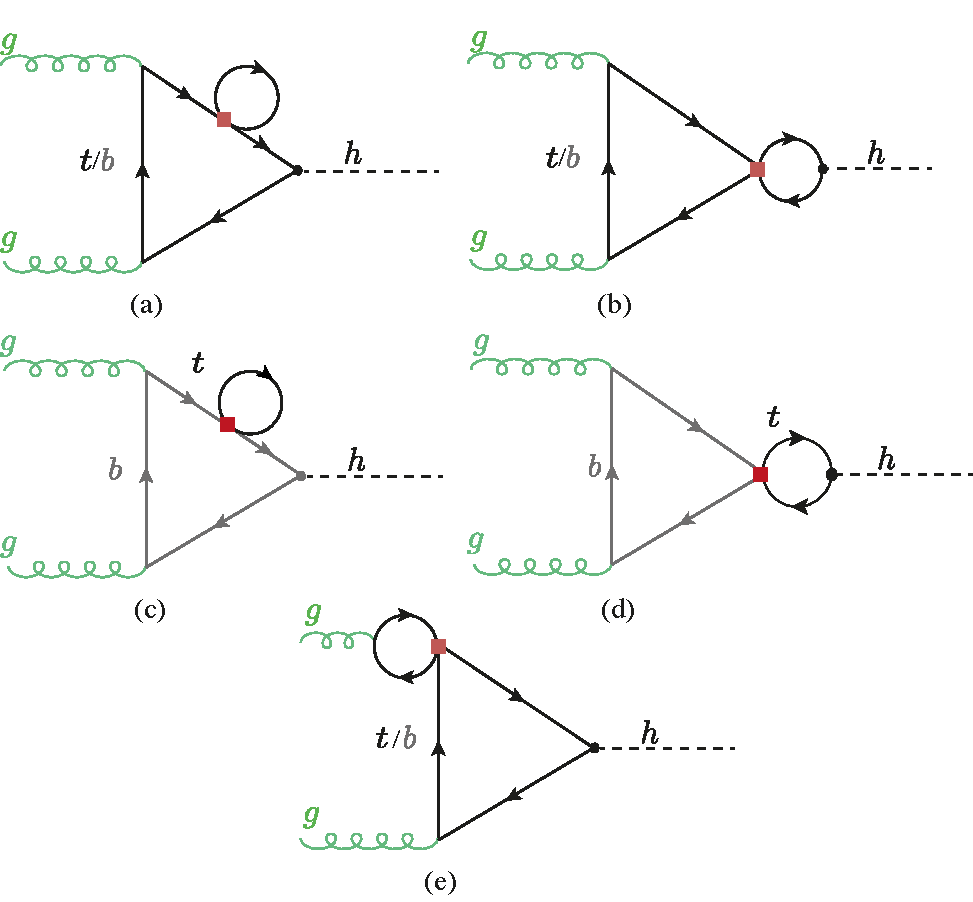
\includegraphics[width=12cm]{fig/ggF-4F_NLO.pdf}
		\caption{Example Feynman diagrams for four-fermion-operator contributions to the Higgs production via gluon fusion. The red box indicates the four-fermion operator.\label{fig:ggh} }
	\end{center}
\end{figure}
The first and second type of corrections are left-right (LR) transitions hence the only contributions stem from the operators with Wilson coefficients $C_{Qt}^{(1),(8)}$ and $C^{(1),(8)}_{QtQb}$.
As can be inferred from the diagrams in \autoref{fig:ggh} the result can be expressed as a product of one-loop integrals. We computed the diagrams in two independent calculations making use of different computer algebra tools such as \texttt{PackageX} \cite{Patel:2015tea}, \texttt{KIRA} \cite{Maierhoefer:2017hyi}, \texttt{Fire} \cite{Smirnov:2008iw}, \texttt{FeynRules} \cite{Alloul:2013bka} and \texttt{FeynArts} \cite{Hahn:2000kx}.\footnote{Note that the latter tool needed some manual adjustments to deal with four-fermion operators.}  
We cross-checked the Feynman rules with ref.~\cite{Dedes:2017zog}.
\\
For the renormalisation procedure we adopt a mixed on-shell (OS)-$\MSbar$ -- scheme as proposed in \cite{Dawson:2018pyl}, in which we renormalise 
the quark masses OS and the Wilson coefficients of the dimension-six operators using  the $\MSbar$\;scheme. 
We hence renormalise the top/bottom mass as
\begin{equation}
	m_{t/b}^{\text{OS}}=m_{t/b}^{(0)}-\delta m_{t/b},
\end{equation}
%
where the counterterms are given by
\begin{align}
	\delta m_t =&\frac{1}{16 \pi^2} \frac{C_{Qt}^{(1)}+c_F C_{Qt}^{(8)}}{\Lambda^2}m_t^3\left[ \frac{2}{\bar{\epsilon}} +2 \log\left(\frac{\mu_R^2}{m_t^2}\right)+1\right] \\ &+ \frac{1}{16 \pi^2}  \frac{(2 N_c+1) C_{QtQb}^{(1)}+c_F C_{QtQb}^{(8)}}{\Lambda^2}  \left[ \frac{1}{\bar{\epsilon}} +  \log\left(\frac{\mu_R^2}{m_b^2}\right)+1 \right]  m_b^3\,, \nonumber \\
	\delta m_b=&\frac{1}{16 \pi^2} \frac{(2 N_c+1)C_{QtQb}^{(1)}+c_F C_{QtQb}^{(8)}}{\Lambda^2}\left[ \frac{1}{\bar{\epsilon}} +\log\left( \frac{\mu_R^2}{m_t^2}\right)+1\right] m_t^3\,,
\end{align}
with $\bar{\epsilon}^{-1} = \epsilon^{-1}- \gamma_E +\log(4 \pi)$, in dimensional regularization with $d=4-2\epsilon$, $N_c=3$ the number of colors, and $c_F=(N_c^2-1)/(2N_c)=4/3$ the $SU(3)$ quadratic Casimir in the fundamental representation. 
We note that, for the calculations of the physical processes in this paper, the difference between using the OS or the $\MSbar$\;definitions of the top and bottom masss in SMEFT results in changes that are formally of $\mathcal{O}(1/\Lambda^4)$.\footnote{In the $\MSbar$\;scheme the mass counterterms become
	\begin{align}
		\delta m_t^{\bar{\text{MS}}} =&\frac{1}{8 \pi^2} \frac{C_{Qt}^{(1)}+c_F C_{Qt}^{(8)}}{\Lambda^2}m_t^3\frac{1}{\bar{\epsilon}}+ \frac{1}{16 \pi^2}  \frac{(2 N_c+1) C_{QtQb}^{(1)}+c_F C_{QtQb}^{(8)}}{\Lambda^2}   \frac{1}{\bar{\epsilon}}  m_b^3\,,  \\
		\delta m_b^{\bar{\text{MS}}}=&\frac{1}{16 \pi^2} \frac{(2 N_c+1)C_{QtQb}^{(1)}+c_F C_{QtQb}^{(8)}}{\Lambda^2}\frac{1}{\bar{\epsilon}} m_t^3\,.
	\end{align}
}
We note though that using a SM running $\MSbar$\;bottom mass instead of an OS one makes a relevant difference in the numerical results.
In the results presented below we will use the OS bottom mass as an input.

The coefficients of the dimension-six operators 
are renormalised in the $\MSbar$ \;scheme.
At one-loop level the only operators entering the Higgs to gluon or photon rates that mix with the four-quark operators are the ones that modify the top or bottom Yukawa couplings: ${\cal O}_{t\phi}$ and ${\cal O}_{b\phi}$, respectively. The coefficients of these operators are renormalized according to
\begin{equation}
	C^{\bar{\text{MS}}}_{t\phi/b\phi}=C^{(0)}_{t\phi/b\phi}+\delta C_{t\phi/b\phi}\quad\quad \text{   with   }\quad\quad \delta C_{t\phi/b\phi} = -\frac{1}{2\bar{\epsilon}}\frac{1}{16 \pi^2} \gamma^{j}_{t\phi/b\phi} C_j.
\end{equation}
The only four-quark Wilson coefficients contributing to $\gamma_{t\phi/b\phi}$ are the ones from ${\cal O}_{Qt}^{(1),(8)}$ and  ${\cal O}_{QtQb}^{(1),(8)}$. 
The explicit expressions for the relevant one-loop anomalous dimension can be obtained from ref.~\cite{Jenkins:2013zja,Jenkins:2013wua}. 
The Wilson coefficients $C_{t\phi/b\phi}$ modify the Higgs couplings to top quarks/bottom quarks as follows
\begin{equation}
	g_{ht\bar{t}/hb\bar{b}}=\frac{m_{t/b}}{v}-\frac{v^2}{\Lambda^2}\frac{C_{t\phi/b\phi}}{\sqrt{2}}\,.
\end{equation}
Hence, a modification of the Higgs couplings to bottom and top quarks is generated by operator mixing, even if $C_{t\phi/b\phi}$ are zero at $\Lambda$.
\par
The modification of the Higgs production rate in gluon fusion (ggF) can be written as
\begin{equation}
	\frac{\sigma_{ggF}}{\sigma_{ggF}^{\SM}}= 1+ \frac{ \sum_{i=t,b} 2 \Re(F_{\LO}^i F^*_{\NLO})}{\left| F_{\LO}^t+F_{\LO}^b  \right|^2} \label{eq:production}
\end{equation}
with 
%
\begin{equation}
	F_{\LO}^i=-\frac{8m_i^2}{m_h^2}\left[1-\frac{1}{4}\log^2(x_i)\left(1-\frac{4m_i^2}{m_h^2}\right)\right]
\end{equation}
where $m_h$ is the Higgs mass,
and
%
\begin{equation}
	\begin{split}
		F_{\NLO}=&\frac{ 1}{4\pi^2  \Lambda^2}(C_{Qt}^{(1)}+c_FC_{Qt}^{(8)})F_{\LO}^t \left[ 2 m_t^2  +\frac{1}{4} (m_h^2-4 m_t^2) \left( 3 +2 \sqrt{1-\frac{4 m_t^2}{m_h^2}} \log(x_t) \right)  \right. \\ & \left.
		+\frac{1}{2} (m_h^2-4 m_t^2) \log\left(\frac{\mu_R^2}{m_t^2}\right)\right] \\ & + 
		\frac{1}{32 \pi^2 \Lambda^2} ((2N_c+1)C_{QtQb}^{(1)}+c_FC_{QtQb}^{(8)}) \left[ F_{\LO}^b \frac{m_t}{m_b}\left( 4 m_t^2-2 m_h^2 \right. \right.\\ & \left. \left. - (m_h^2-4 m_t^2)\sqrt{1-\frac{4 m_t^2}{m_h^2}} \log(x_t)-(m_h^2-4 m_t^2)\log\left(\frac{\mu_R^2}{m_t^2}\right)\right) +(t\leftrightarrow b)\right]  \,. \label{eq:FNLO}
	\end{split}
\end{equation}
Only top quark loops contribute to the parts proportional to $C_{Qt}^{(1),(8)}$. We have neglected the contributions of the operators with Wilson coefficient $C_{Qb}^{(1),(8)}$ as they would lead only to subleading contributions proportional to $m_b^3$.
%
The variable $x_i$ for a loop particle with mass $m_i$ is given by
\begin{equation}
	x_i=\frac{-1+\sqrt{1-\frac{4 m_i^2}{m_h^2}}}{1+\sqrt{1-\frac{4 m_i^2}{m_h^2}}}\,. \label{eq:xvariable}
\end{equation} 
In analogy to \eqref{eq:production}, we can write the modified decay rates of the Higgs boson to gluons as
\begin{equation}
	\frac{\Gamma_{h\to gg}}{\Gamma_{h\to gg}^{\SM}}= 1+ \frac{ \sum_{i=t,b} 2 \Re(F_{\LO}^i F^*_{\NLO})}{ |F_{\LO}^t+F_{\LO}^b|^2} 
\end{equation}
and 
\begin{equation}
	\frac{\Gamma_{h\to \gamma\gamma}}{\Gamma_{h\to \gamma\gamma}^{\SM}}= 1+ \frac{2 \Re(F_{\LO, \gamma} F^*_{\NLO,\gamma})}{  |F_{\LO, \gamma}|^2} .
\end{equation}
In the latter 
\begin{equation}
	F_{\LO, \gamma}= N_C\,Q_t^2 F_{\LO}^t+ N_C\,Q_b^2 F_{\LO}^b+F_{\LO}^W+ F^G_{LO} ,
\end{equation}
and $F_{\NLO, \gamma}$ is obtained from $F_{\NLO}$ by replacing the LO form factor that appears inside of it by  $ F_{\LO}^i \to N_c \,Q_i^2 F_{\LO}^i$,
with the charges $Q_t=2/3$ and $Q_b=-1/3$. The $W$ boson contribution
%
\begin{equation}
	F_{\LO}^W= 2 \left(1+6 \frac{m_W^2}{m_h^2}\right)-6 \frac{m_W^2}{  m_h^2} \left(1-2  \frac{m_W^2}{m_h^2}\right) \log^2(x_W),
\end{equation}
with $m_W$ the $W$ mass, and the Goldstone contribution
%
\begin{equation}
	F_{\LO}^G=4\frac{m_W^2}{m_h^2} \left( 1+ \frac{m_W^2}{m_h^2} \,\log^2(x_W) \right)\,.
\end{equation}
\par

The formulae presented above are valid under the assumption that, at the electroweak scale, the four-quark operators are the only new physics contributions in the dimension-six effective Lagrangian. If, on the other hand, one assumes that the four-quark operators are defined at some high scale $\Lambda$, e.g.~after matching with an specific ultraviolet (UV) model, further (logarithmic) contributions appear during the running to low energies, as a result of the mixing between these four-fermion interactions and those operators that would modify the processes at LO. 
Those effects can be included via the renormalisation group equation (RGE) for the operators with Wilson coefficient $C_{t\phi}$  and $C_{b\phi}$  \cite{Jenkins:2013zja, Jenkins:2013wua}, that lead approximatively to 
\begin{equation}
	\begin{split}
		C_{t\phi}(\mu_R)-C_{t\phi}(\Lambda)= &\frac{1}{16 \pi^2 v^2} \left[-2  y_t (m_h^2  -4 m_t^2) (C_{Qt}^{(1)}+c_F C_{Qt}^{(8)} )\log\left( \frac{\mu_R^2}{\Lambda^2}\right) \right.\\
		& \left.+ \frac{y_b}{2} (m_h^2-4 m_b^2)\left(  (2N_c+1)  C_{QtQb}^{(1)}+   c_F C_{QtQb}^{(8)}\right)\log\left( \frac{\mu_R^2}{\Lambda^2}\right)\right] \label{eq:runningCuH}
	\end{split}
\end{equation}
and
\begin{equation}
	\begin{split}
		C_{b\phi}(\mu_R)-C_{b\phi}(\Lambda)= \frac{y_t}{32 \pi^2 v^2} \left[  (m_h^2-4 m_t^2)\left(  (2N_c+1)  C_{QtQb}^{(1)}+   c_F C_{QtQb}^{(8)}\right)\log\left( \frac{\mu_R^2}{\Lambda^2}\right)\right]\,, \label{eq:runningCdH}
	\end{split}
\end{equation}
where $y_{t/b}=\sqrt{2} m_{t/b}/v$.
Note that the combinations of Wilson coefficients  appearing in \eqref{eq:runningCuH}\eqref{eq:runningCdH} are the same as in $F_{NLO}$ in \eqref{eq:FNLO}.
Effectively, we can then obtain the result under the assumption that the four-fermion operators are the only non-zero ones at the high scale by replacing in \eqref{eq:FNLO} $\mu_R \to \Lambda$, noting that we have renormalised the top and bottom quark mass in the OS scheme.
%%%%%%%%%%%%%%%%%%%%%%%%%%%%%%%%%%%%%%%%%%%%%%%%%%%%%%%%%%%%%%%%%%%%%%%%

\subsection{Higgs decay to bottom quarks}
\begin{figure}[t!]
	\vspace{-.5 cm}
	\centering
	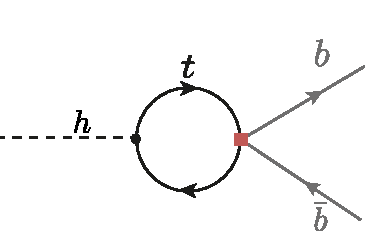
\includegraphics[scale=0.85]{./fig/Hbb}
	\caption{Feynman diagram contributing to the NLO   $h \to b \bar b$ process. }
	\label{hbb}
\end{figure}
The dominant four-fermion contributions to decay channel $h \to b\bar b$ come from the operators with Wilson coefficients $C_{QtQb}^{(1),(8)}$. The corresponding diagram at NLO is shown in~fig~\ref{hbb}. 
Adopting the same renormalisation procedure as outlined in the previous subsection, we obtain the following expression for the correction to 
the $h \to b\bar b$ decay rate in the presence of ${\cal O}_{QtQb}^{(1),(8)}$,
\begin{equation}
	\begin{split}
		\frac{\Gamma_{h\to b\bar{b}}}{\Gamma_{h\to b\bar{b}}^{\SM}}=& 1+ \frac{1}{16\pi^2}\frac{m_t}{m_b}(m_h^2-4m_t^2)\frac{(2 N_c+1) C_{QtQb}^{(1)}+c_F C_{QtQb}^{(8)}}{\Lambda^2} \\ & \times\left[ 2+\sqrt{1-\frac{4 m_t^2}{m_h^2}}\log(x_t)-\log\left(\frac{m_t^2}{\mu_R^2}\right) \right] \,,
		\label{hbbnlo}
	\end{split}
\end{equation}
which carries an enhancement factor of $m_t/m_b$ and is hence expected to be rather large.
Again, we have neglected subdominant contributions suppressed by the bottom mass from the operators $\mathcal{O}_{Qb}^{(1),(8)}$. 
Including the leading logarithmic running of $C_{b\phi}$ of \eqref{eq:runningCdH} from the high scale $\Lambda$ to the electroweak scale is achieved by setting in \eqref{hbbnlo} $\mu_R\to \Lambda$.
The expression in \eqref{hbbnlo} agrees with results obtained from the full calculation of the NLO effects in the dimension-six SMEFT, first computed in~\cite{Gauld:2015lmb}. 

This closes the discussion of the main effects that the third-generation four-quark operators can have in the different Higgs decay widths.\footnote{Four-fermion operators also affect the $h\to Z\gamma$ partial width. However, as in the diphoton case, the effect is expected to be small due to the dominance of the $W$ boson loop. Because of this, and given the smallness of the $h\to Z\gamma$ branching ratio and the relatively low precision expected in this channel at the LHC, we neglect the effects of four-fermion interactions in this decay.} Note also that these modifications of the Higgs decay rate to photons, gluons and, especially, bottom quarks, affect all the branching ratios (BRs) due to the modification of the Higgs total width, and therefore have an observable effect in all Higgs processes measured at the LHC.

%%%%%%%%%%%%%%%%%%%%%%%%%%%%%%%%%%%%%%%%%%%%%%%%%%%%%%%%%%%%%%%%%%%%%%%%

\subsection{Associated production of a Higgs boson with top quarks}

\begin{figure}[t!]
	\centering
	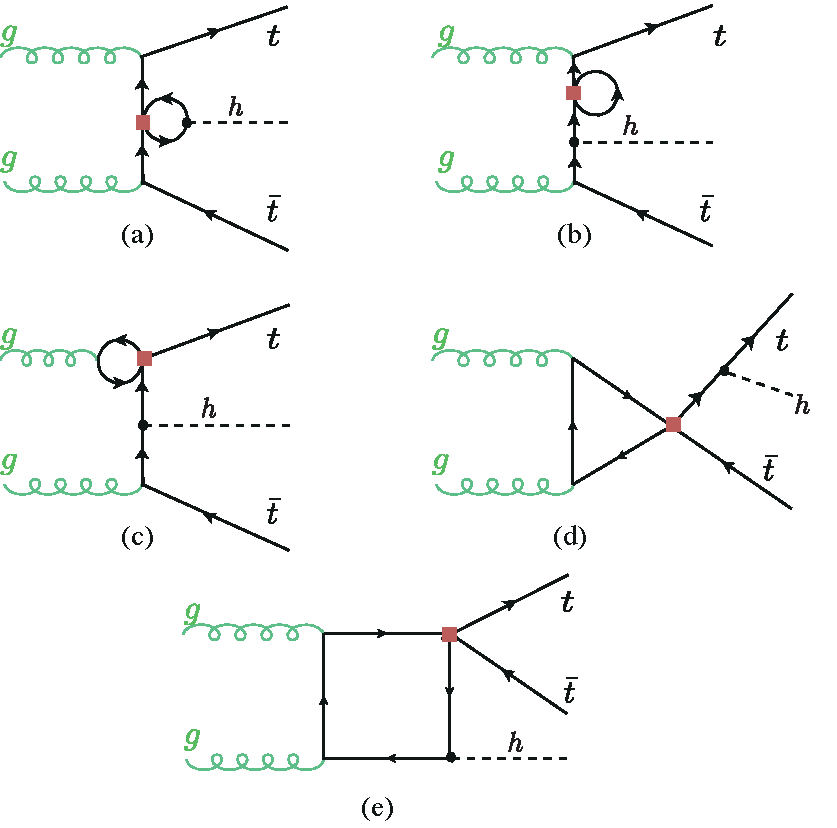
\includegraphics[scale=0.85]{./fig/ggttH-4F_NLO}
	\caption{Feynman diagrams including the four-fermion loop contributions to the $ gg \to t\bar{t} h$ subprocess.}
	\label{ggtth}
\end{figure}
\begin{figure}[ht!]
	\centering
	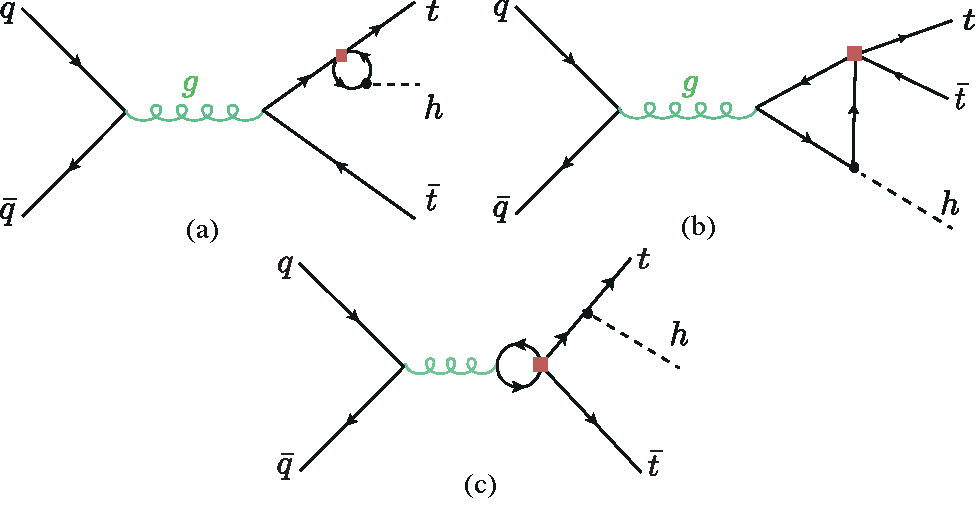
\includegraphics[scale=0.85]{./fig/qqttH-4F_NLO}
	\caption{Feynman diagrams including the four-fermion loop contributions to the  $ q \bar{q} \to t\bar{t} h$ subprocess.}
	\label{qqtth}
\end{figure}

The associated Higgs production with top quarks, $t\bar{t}h$, receives significant  NLO corrections from the singlet and octet operators $\mathcal{O}_{Qt}^{(1),(8)}$, while the contributions from $\mathcal{O}_{QtQb}^{(1),(8)}$ remain small. In addition, there are some small contributions from the singlet and triplet left-handed operators, $\mathcal{O}_{QQ}^{(1),(3)}$, and the right-handed four-top operator, $\mathcal{O}_{tt}$, as well.
The $ t\bar{t} h$ process can be either initiated by gluons, see \autoref{ggtth}, or by a quark anti-quark pair, see \autoref{qqtth}.  The triangle and box topologies (shown as (d) and (e) in \autoref{ggtth} and as (b) in \autoref{qqtth}) are finite. While for Higgs production/decay in/to gluons only certain combinations of singlet/octet operators entered, leading to a degeneracy, this is not the case for $t\bar{t}h$ production, where the gluons no longer need to combine to a colour singlet state. 
The degeneracy between the singlet and octet operators is mainly broken by the contributions from the triangle diagrams, where, for instance, the difference between the contributions of $\mathcal{O}_{Qt}^{(1)}$ and $\mathcal{O}_{Qt}^{(8)}$ does not follow the same color structure as other diagrams.

We adopt a four-flavour scheme for the computation of the quark-initiated contributions. We note that within a five-flavour scheme operators containing both bottom and top quarks lead to a LO contribution from a direct contact diagram. Nevertheless, this gives an overall negligible correction as the $ b \bar b $ initiated $t\bar t h$ process is suppressed by the small bottom parton distribution functions. The effect of changing the flavour scheme results in an uncertainty of $1-2\%$.
\par
We have computed the NLO corrections using \texttt{Madgraph\_aMCNLO} \cite{Alwall:2014hca} (version  3.1.0) with the \texttt{SMEFTatNLO v1.0.2} model~\cite{Degrande:2020evl}. The results were cross-checked by an analytic computation\footnote{The \texttt{ FORTRAN} code containing this analytical calculation can be provided on request.}, based on the reduction of one-loop amplitudes via the method developed by G. Ossola, C.G. Papadopoulos and R. Pittau~(OPP reduction)~\cite{Ossola:2006us}.
The OPP reduction was done using the \texttt{CutTools} programme~\cite{Ossola:2007ax}.
%
It reduces the one-loop amplitude into 1,2,3 and 4-point loop functions in four dimensions, keeping spurious terms from the $\epsilon$ part of the amplitude. To correct for such terms, one needs to compute the divergent UV counterterm as well as a finite rational terms, denoted $R_{2}$ as in Ref.~\cite{Ossola:2008xq}.\footnote{Another rational term ~$R_1$ appears due to the mismatch between the four and $d$ dimensional amplitudes, but this is computed automatically in \texttt{CutTools}. } The amplitudes were generated in the same way as for gluon fusion. The UV and $R_2$ counterterms, that need to be supplemented to \texttt{CutTools}, were computed manually following the method detailed in~\cite{Ossola:2008xq}.
The UV counterterms are the same as for gluon fusion, in addition to a new one  that is needed to be introduced to renormalise diagrams of type (c) in \autoref{ggtth} and \autoref{qqtth}. This is due to the operator mixing of light -- heavy four-quark operators with heavy four-quark operators. Effectively, this leads to a counterterm 
\begin{equation}
	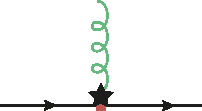
\includegraphics[width=0.13\linewidth]{fig/CT} =\frac{ig_s}{12 \pi^2\Lambda^2} T^{A}_{ij} p_g^2 \gamma^\mu \left( C_{tt} P_R+\left(C_{QQ}^{(1)} + C_{QQ}^{(3)}\right) P_L +\frac{ C_{Qt}^{(8)}}{4} \right) \left( \frac{1}{\bar{\epsilon}}-1 \right) . \label{eq:R2CT}
\end{equation}
%
Since the singlet and octet operators $\mathcal{O}_{QtQb}^{(1),(8)}$ are not implemented in the current version of \texttt{SMEFTatNLO}, or in any other loop-capable \texttt{UFO} model available, we have modified the \texttt{SMEFTatNLO} model to include these operators, by including their Feynman rules and computing the UV and $R_2$ counterterms needed for the $t\bar t h$ calculation. 
These $\mathcal{O}_{QtQb}^{(1),(8)}$ contributions are included for consistency, as they were relevant and thus included in the calculation of, e.g. $h\to b\bar{b}$. However, as we will argue below, their contribution to $t\bar{t}h$ is rather small. Similarly, other ``mixed'' bottom-top operators are expected
to give also suppressed contributions, compared to those from four-top operators. Therefore we neglect their effects in our calculation.\footnote{Furthermore, we note that such operators are also currently not included in \texttt{SMEFTatNLO}. A computation of their contributions, while being beyond the scope of this paper, would require a similar strategy as for the $\mathcal{O}_{QtQb}^{(1),(8)}$ operator.}

Again, to connect with specific models that may generate the four-quark operators at the new physics scale $\Lambda$, one needs to consider the contributions that come from the running from $\Lambda$ to low energies, and that mix these operators with those entering in $t\bar{t}h$ at the LO level. 
For the gluon-initiated subprocess the relevant contributions are from the running of $C_{t\phi}$ in \eqref{eq:runningCuH}, while for the quark-initiated subprocess we need to account for the mixing of the third generation four-fermion operators with the ones connecting the third generation with the first two generations. The corresponding corrections can be obtained from the RGEs in refs. \cite{Jenkins:2013zja,Jenkins:2013wua,Alonso:2013hga}.

%%%%%%%%%%%%%%%%%%%%%%%%%%%%%%%%%%%%%%%%%%%%%%%%%%%%%%%%%%%%%%%%%%%%%%%%

\subsection{Results}

Here we provide semi-analytical expressions for the results of our NLO calculations including the effects of the third generation four-quark operators. 
These NLO contributions to the single Higgs rates, as a function of the four-heavy-quark Wilson coefficients, are denoted by
\begin{equation}
	\delta R(C_i) = R/R^{\SM} -1,
	\label{eq:deltaR}
\end{equation}
where $R$ stands generically for partial width $\Gamma$ or cross section $\sigma$. They are summarised in~\autoref{table:res4top}. 
The numbers consider only the linear contributions in $\Lambda^{-2}$.  
The respective $\delta R(C_i) $ get a contribution from the computation of the finite corrections to the process and an additional contribution from operator mixing due to RGE running and can hence be split into two parts
\begin{equation}
	\delta R(C_i)= \frac{C_i}{\Lambda^2}\left(\delta R_{C_i}^{fin}+ \delta R_{C_i}^{log} \log\left(\frac{\mu_R^2}{\Lambda^2}\right)\right)\,.
	\label{eq:deltar}
\end{equation}
%
We note that the way we write our results corresponds to the finite part of the NLO correction taken at a typical process scale $\mu_R$ and a contribution obtained by solving the RGE of the dimension-six Wilson coefficients via the leading log approximation from the high scale $\Lambda$ to the low scale $\mu_R$.  Both the finite part dependence $\delta R_{C_i}^{fin}$ of these corrections on the  Wilson coefficient as well as the part proportional to the logarithm $\delta R_{C_i}^{log}$  are reported in table~\ref{table:res4top}.
Our results can be improved by replacing the part proportional to the coefficients  $\delta R^{log}_{C_i}$ by solving the coupled system of RGEs. 
For $ \Lambda =1$ TeV, and depending on the renormalisation scale of the process, the value of the logarithm in \eqref{eq:deltar} ranges between $\sim[-5.5,-2.9]$. With these numerical values in mind and by looking at $\delta R_{C_i}^{log}$ in table~\ref{table:res4top}, we see that the finite part of the NLO calculation, i.e. $\delta R_{C_i}^{fin}$, is usually of the same order  of magnitude or larger than the leading-log part, with the exception of the $C_{QtQb}^{(1),(8)}$ contributions to the $h\to b\bar{b}$. This underlines the importance of considering the full NLO computation in the determination of the Wilson coefficients for $C_{Qt}^{(1),(8)}$, whereas for $C_{QtQb}^{(1),(8)}$, where the limits are mainly driven by $h\to b\bar{b}$, they turn out to play less important role.

\begin{table}[t!]
	\centering
	\small{
		\begin{tabular}{c||cccc}
			\toprule
			{ \normalsize Operator} &  { \normalsize Process }& { \normalsize $\mu_R$} & { \normalsize$ \delta R_{C_i}^{fin}\; [\text{TeV}^2]$} &{ \normalsize$ \delta R_{C_i}^{log}\; [\text{TeV}^2] $} \\
			\midrule
            \multirow{5}{*}{ { \normalsize$\mathcal{O}_{Qt}^{(1)}$}}  &  ggF& $\frac{m_h}{ 2}$&$\phantom{+}9.91\cdot 10^{-3}$&$\phantom{+}2.76\cdot 10^{-3}$\\     % \cmidrule(r){2-5}  
                                                                    &  $h \to gg$& \mr{$m_h$}&$\phantom{+}6.08\cdot 10^{-3}$&$\phantom{+}2.76\cdot 10^{-3}$\\
            	                                                   &  $h \to \gamma \gamma$& &$-1.76\cdot 10^{-3}$ &$-0.80\cdot 10^{-3}$ \\
            	                                              %     \cmidrule(r){2-5}    
            	                                                   	&  $t\bar t h$ {\color{Mahogany}  13 TeV }&\mr{ $m_t+\frac{m_h}{ 2}$}&$-4.20\cdot 10^{-1} $&$-2.78\cdot 10^{-3}$\\	    
            	                                                   	&   $t\bar t h$  {\color{Mahogany}  14 TeV }& &$-4.30\cdot 10^{-1} $&  $-2.78\cdot 10^{-3}$\\	
            	                                                   	\midrule
          \multirow{5}{*}{ { \normalsize$\mathcal{O}_{Qt}^{(8)}$} } & ggF& {$\frac{m_h}{ 2}$}&$\phantom{+}1.32\cdot 10^{-2}$&$\phantom{+}3.68\cdot 10^{-3}$\\    %  \cmidrule(r){2-5}  
                                                                   &  $h \to gg$& \mr{$m_h$}&$\phantom{+}8.11\cdot 10^{-3}$&$\phantom{+}3.68\cdot 10^{-3}$\\
            	                                                   	&  $h \to \gamma \gamma$& &$-2.09\cdot 10^{-3}$&$-1.07\cdot 10^{-3}$\\
            	                                                   %	 \cmidrule(r){2-5}    
            	                                                   	&  $t\bar t h$ {\color{Mahogany}  13 TeV }& \mr{$m_t+\frac{m_h}{ 2}$}&$\phantom{+}6.81\cdot 10^{-2}$ &$-2.40\cdot 10^{-3}$\\	    
            	                                                   	&   $t\bar t h$  {\color{Mahogany}  14 TeV }& & $\phantom{+}7.29\cdot 10^{-2}$&  $-2.48\cdot 10^{-3}$\\	              
                       	                                                   	\midrule
           \multirow{4}{*}{ { \normalsize$\mathcal{O}_{QtQb}^{(1)}$} } & ggF& ${m_h\over 2}$&$\phantom{+}2.84\cdot 10^{-2}$&$\phantom{+}9.21\cdot 10^{-3}$\\   %   \cmidrule(r){2-5}  
            &  $h \to gg$& \multirow{3}{*}{$m_h$}&$\phantom{+}1.57\cdot 10^{-2}$&$\phantom{+}9.21\cdot 10^{-3}$\\
           &  $h \to \gamma \gamma$& &$-1.30\cdot 10^{-3}$&$-0.78\cdot 10^{-3}$\\
           &  $h \to b \bar b$& &$\phantom{+}9.25\cdot 10^{-2}$&$\phantom{+}1.68\cdot 10^{-1}$\\
         %   \cmidrule(r){2-5}    
			\midrule
			 \multirow{4}{*}{{ \normalsize$\mathcal{O}_{QtQb}^{(8)}$}}  & ggF& {$\frac{m_h}{ 2}$}&$\phantom{+}5.41\cdot 10^{-3}$&$\phantom{+}1.76\cdot 10^{-3}$\\      %\cmidrule(r){2-5}  
			 & $h \to gg$& \multirow{3}{*}{$m_h$}&$\phantom{+}2.98\cdot 10^{-3}$&$\phantom{+}1.76\cdot 10^{-3}$\\
			&  $h \to \gamma \gamma$& &$-0.25\cdot 10^{-3}$& $-0.15\cdot 10^{-3}$\\
			&  $h \to b \bar b$& &$\phantom{+}1.76\cdot 10^{-2}$&$\phantom{+}3.20\cdot 10^{-2}$\\
			% \cmidrule(r){2-5}    
			\midrule	    	 
			 \multirow{2}{*}{{ \normalsize$\mathcal{O}_{QQ}^{(1)}$}  }
			 	&  $t\bar t h$ {\color{Mahogany}  13 TeV }& \mr{$m_t+\frac{m_h}{ 2}$}&  {$\phantom{+}1.75\cdot 10^{-3}$} &$\phantom{+}1.84\cdot 10^{-3}$\\	    
			 &   $t\bar t h$  {\color{Mahogany}  14 TeV }& & $\phantom{+}1.65\cdot 10^{-3}$& $\phantom{+}1.76\cdot 10^{-3}$\\          
			 \midrule	    	 
			 \multirow{2}{*}{{ \normalsize$\mathcal{O}_{QQ}^{(3)}$}  }
			 &  $t\bar t h$ {\color{Mahogany}  13 TeV }& \mr{$m_t+\frac{m_h}{ 2}$}&  $\phantom{+}1.32\cdot 10^{-2}$ & $\phantom{+}5.48\cdot 10^{-3}$\\	    
			 &   $t\bar t h$  {\color{Mahogany}  14 TeV }& & $\phantom{+}1.24\cdot 10^{-2}$& $\phantom{+}5.30\cdot 10^{-3}$\\        
			  \midrule	    	 
			 \multirow{2}{*}{{ \normalsize$\mathcal{O}_{tt}$}  }
			 &  $t\bar t h$ {\color{Mahogany}  13 TeV }& \mr{$m_t+\frac{m_h}{ 2}$}&  $\phantom{+}4.60\cdot 10^{-3}$ &$\phantom{+}1.82\cdot 10^{-3}$\\	    
			 &   $t\bar t h$  {\color{Mahogany}  14 TeV }& & $\phantom{+}4.57\cdot 10^{-3}$& $\phantom{+}1.74\cdot 10^{-3}$\\                                           	
			\bottomrule
		\end{tabular}
	}
\caption{The NLO effects of the four heavy-quarks operators on the Higgs rates. The effects are separated into finite ~$ \delta R_{C_i}^{fin}$ and leading log~ parts, in correspondence with~\eqref{eq:deltar}.  This table has been published in~\cite{Alasfar:2022zyr}.}
\label{table:res4top}
\end{table}


The numerical values were obtained using as input parameters
\begin{equation}
	\begin{split}
		& G_F=1.166378 \cdot 10^{-5} \text{ GeV}^{-2}\,,  \; m_W=80.379\text{ GeV}\,, \;m_Z=91.1876\text{ GeV}\,, \\ &  m_t^{\text{OS}}=172.5 \text{ GeV}\,, \; m_b^{\text{OS}}=4.7\text{ GeV}\,,  \;m_h=125.1\text{ GeV}\,,
	\end{split}
\end{equation}
and the NNPDF23 set at NLO \cite{Ball:2012cx}. 

Looking at the results, first we note that the operators ${\cal O}_{QQ}^{(1),(3)} $ and ${\cal O}_{tt}$ only contribute to $t\bar t h$ production. 
In this regard, however, it must be noted that the uncertainties of the renormalisation schemes, the scale uncertainty, the PDF+$\alpha_s$ uncertainty and the one of the flavour schemes of the $t\bar t h$ process are~$ \sim 5\%$. This is larger than the typical effects of $C_{QQ}^{(1),(3)} $ and $C_{tt}$ for ${\cal O}(1)$ coefficients. Therefore, all Higgs rates are expected to be relatively insensitive to these interactions 
unless rather large values of these Wilson coefficients are allowed.  
Secondly, from the analytic results, we observe that in the NLO corrections to Higgs rates, the Wilson coefficients $C_{QtQb}^{(1)} ,  C_{QtQb}^{(8)}$ always appear in a linear combination identical to the one seen in the RGE of the Wilson coefficients~$C_{t\phi}$ and~$C_{b\phi}$, i.e. 
%
\begin{equation}
	C_{QtQb}^+= (2N_c+1 )C_{QtQb}^{(1)} + c_F   C_{QtQb}^{(8)}.
	\label{eq:CQtQbplus}
\end{equation}
%
The exception is the $t\bar t h$ process, which has a small finite part contribution that breaks this relation. However, this finite part is suppressed by the bottom quark mass and therefore it is very small. Thus, all single Higgs rates are mostly sensitive to the linear combination in \eqref{eq:CQtQbplus}.
We finally note that apart from $\mathcal{O}_{Qt}^{(1),(8)}$ all the other operators produce only small contributions to the $t\bar{t}h$ process. In particular, the top-bottom operators $\mathcal{O}_{QtQb}^{(1),(8)}$ show a suppression with $m_b$, which also typically results in contributions below the theoretical uncertainties. (We explicitly checked this in our calculation and by setting $m_b=0$ in the \texttt{Madgraph\_aMCNLO} simulations.)  This is also expected for other ``mixed" top-bottom operators,
which would contribute via bottom-quark loops and hence would be strongly suppressed, justifying that we did not consider them here. 

%%%%%%%%%%%%%%%%%%%
\section{Fit to Higgs observables \label{sec:fit}}
%%%%%%%%%%%%%%%%%%%

\par In this section we will show the results of a combined fit of the four-quark operators of the third generation and the operator that modifies the Higgs potential and hence the Higgs self-coupling. In ref.~\cite{Gorbahn:2016uoy, Degrassi:2016wml, Bizon:2016wgr, Maltoni:2017ims, Degrassi:2021uik} it was proposed to extract the trilinear Higgs self-coupling via its loop effects in single Higgs measurements. 
%
Within the assumptions of the SMEFT, a model-independent determination of the triple Higgs self-interaction, $\lambda_3$, should be considered within a global analysis considering all effective interactions that enter up to the same order in perturbation theory as $\lambda_3$.
In particular, apart from the trilinear Higgs self-coupling modification, such a study must include those operators that enter at LO in Higgs production and decay~\cite{DiVita:2017eyz}. Furthermore, the sensitivity to the Higgs self-coupling modifications can also be diminished by other operators entering as the trilinear Higgs self-coupling via loop effects, if those operators are not yet strongly constrained experimentally by other processes. Such is the case for some of the four-quark operators considered in this paper. In order to show this, we have performed a combined fit to the operator with Wilson coefficient $C_{\phi}$ and the four-fermion operators considered in this study. A full global fit including all new physics effects would require the combination of Higgs data with that from other processes and is beyond the scope of this paper. 

\subsection{Fit methodology}
%

For each experimentally observed channel with a signal strength~$\mu_{\mathrm{Exp}}\equiv \sigma_{\mathrm{Obs}}/\sigma_\SM$, one can build a theoretical prediction for this signal strength, $\mu_{\mathrm{Th}}\equiv \sigma_{\mathrm{Th}}/\sigma_\SM$, where $\sigma_{\mathrm{Th}}=\sigma_{\mathrm{Prod}}\times \mathrm{BR}$ includes the effects generated by the dimension-six operators. 
The theory predictions for the signal strengths are then used to build a test statistic in the form of  a $\log$-likelihood of a Gaussian distribution 
\begin{equation}
	\log(L) = -\frac{1}{2}\left[  (\vec{\mu}_{\mathrm{Exp}} -\vec{\mu} ) ^{T} \cdot \mathbf{V}^{-1} \cdot ( \vec{\mu}_{\mathrm{Exp}} -\vec{\mu} )\right]  .
	\label{eq:loglike}
\end{equation}
The covariance matrix~$\mathbf{V}$ is constructed from the experimental uncertainties $\delta \mu_{\mathrm{Exp}}$ and correlations\footnote{Correlations amongst channels of $< 10\%$ were ignored.},  as well as the theoretical uncertainties (scale, PDF, $\alpha_s$, \ldots).

The $\log$-likelihood of \eqref{eq:loglike} was used together with flat priors~$ \pi(C_i)= const.$ in a Bayesian fit of the Wilson coefficients of interest.  A Markov chain Monte Carlo~(MCMC) using \texttt{pymc3}~\cite{Salvatier2016} was used to construct the posterior distribution. We use the \texttt{Arviz} Bayesian analysis package~\cite{arviz_2019} to extract the credible intervals (CIs) from the highest density posterior intervals~(HDPI) of the posterior distributions, where the intervals covering 95\% (68\%) of the posterior distribution are considered the 95\% (68\%) CIs. In the Gaussian limit, these  95\% (68\%) CIs should be interpreted as equivalent to the 95\%  (68\%) Frequentist  Confidence Level~(CL) two-sided bounds. To cross-check the MCMC Bayesian fit, a frequentist Pearson's $\chi^2$ fit was performed using~\texttt{iminuit}~\cite{James:1975dr,iminuit}, where the $\chi^2$ was taken to be 
\begin{equation}
	\chi^2 = - 2 \log(L).
\end{equation}
%
Both fit results agreed on the 95\%  and 68\% CI (or CL)  bounds.\footnote{In order to plot the multidimensional posterior distributions and the forest plots we have used a code based on ~\texttt{corner.py}~\cite{corner}, \texttt{pygtc}~\cite{Bocquet2016} and \texttt{zEpid}~\cite{paul_zivich_2019_3339870}.}
The code for the fit, experimental input and the analysis can be found in the repository \cite{GitHub}.
\par
In the theoretical predictions for the signal strengths, we will assume that the new physics corrections to the cross sections and the decay widths are linearised, i.e.
%
\begin{equation}
	\mu(C_\phi,C_i)=\frac{\sigma_\mathrm{ Prod}(C_\phi,C_i) \times \mathrm{ BR}(C_\phi,C_i)}{\sigma_\mathrm{ Prod, SM}\times \mathrm{BR}_\mathrm{ SM}} \approx 1+\delta \sigma(C_\phi,C_i)+\delta\Gamma(C_\phi,C_i)-\delta \Gamma_h(C_\phi,C_i),
	\label{linear-mu}
\end{equation}
%
with $\delta \sigma$, $\delta \Gamma$, $\delta \Gamma_h$ ($\Gamma_h$ denotes the Higgs total width) being the NLO corrections%to the Higgs full width 
, relative to the SM prediction as in \eqref{eq:deltaR}, 
from the dimension-six operators with Wilson coefficients $C_\phi$ and $C_i$. Here, $C_i$ stands schematically for $C_{Qt}^{(1)}$, $C_{Qt}^{(8)}$, $C_{QtQb}^{(1)}$, $C_{QtQb}^{(8)}$, $C_{QQ}^{(1)}$, $C_{QQ}^{(3)}$ and $C_{tt}$.  As mentioned in the previous section, however, the sensitivity to $C_{QQ}^{(1),(3)}$ and $C_{tt}$ is rather small, typically below the theory uncertainty of the calculation, and we will ignore these Wilson coefficients in the fits presented in this section. 

In particular, in \eqref{linear-mu} all the corrections from the four-quark operators to the cross sections and decay widths are fully linearised in $1/\Lambda^2$. 
Given that current bounds on these operators are rather weak, one may wonder about the uncertainty in our fits associated to the truncation of the EFT.
Note that, since the four-quark operators only enter into the virtual corrections at NLO, Higgs production and decay contain only linear terms in $1/\Lambda^{2}$ in the corresponding Wilson coefficients, i.e.~the quadratic terms coming from squaring the amplitudes are technically of next-to-NLO. 
Hence, the quadratic effects in the signal strengths come from not linearising the corrections to the product $\sigma_\mathrm{ Prod} \times \mathrm{ BR}$~\!.  
We explicitly checked that, for the fits we presented in the next section, the difference between including the full expression of the signal strength or the linearised version in \eqref{linear-mu} results in differences in the bounds at the $\lesssim10\%$ level. The results we present for the four-quark operator are, therefore, relatively stable with respect to the truncation of the EFT expansion. 
For the ${\cal O}_{\phi}$ operator, however, there is an additional contribution to the virtual corrections stemming from the wave function renormalisation of the Higgs field. The correction to a given production cross section or decay width, again denoted generically by $R$, is given by

\begin{equation}
	\delta R_{\lambda_3}\equiv\frac{R_\mathrm{ NLO}(\lambda_3)-R_\mathrm{ NLO}(\lambda_3^\mathrm{{SM}})}{R_\mathrm{ LO}}=-2\frac{C_{\phi}v^4}{\Lambda^2 m_h^2}C_1 + \left(-4\frac{C_{\phi}v^4}{\Lambda^2 m_h^2}+4\frac{C_{\phi}^2 v^8}{m_h^4\Lambda^4}\right) C_2 . \;\;\;\;\;
	\label{eq:degrassi}
\end{equation}
%
In \eqref{eq:degrassi}, the coefficient $C_1$ corresponds to the contribution of the trilinear coupling to the single Higgs processes at one loop, adopting the same notation as~\cite{Degrassi:2016wml}. The values of $C_1$ for the different processes of interest for this paper are given in Appendix~\autoref{App:numinput}. The coefficient $C_2$ describes universal corrections and is given by
\begin{equation}
	C_2=\frac{\delta Z_h}{1-\left(1-\frac{2 C_\phi v^4}{\Lambda^2 m_h^2}\right)^2 \delta Z_h}\,, \label{eq:C2}
\end{equation}
%
where the constant $\delta Z_h$ is the SM contribution from the Higgs loops to the wave function renormalisation of the Higgs boson,
\begin{equation}
	\delta Z_h =-\frac{9}{16}\,\frac{G_F m_h^2}{\sqrt{2}\pi^2}\left(\frac{2\pi}{3\sqrt{3}}-1\right).
\end{equation}
%
The coefficient $C_2$ thus introduces additional $\mathcal{O}(1/\Lambda^4)$ (and higher order) terms in $\delta R_{\lambda_3}$.  
In ref.~\cite{Degrassi:2016wml} considering the $\kappa$ formalism the full expression of \eqref{eq:C2} is kept, while we define two different descriptions: one in which we expand $\delta R_{\lambda_3}$ up to linear order and an alternative scheme in which we keep also terms up to $\mathcal{O}(1/\Lambda^4)$ in the EFT expansion. We explicitly checked that keeping the full expression in \eqref{eq:C2} and including terms up to $\mathcal{O}(1/\Lambda^4)$  in $C_2$ lead to nearly the same results in our fits.


\subsection{Fit to LHC Run-II data}

\par 
For the fit we have used inclusive Higgs data from the LHC Run II for centre-of-mass energy of $\sqrt{s} = 13$ TeV and  integrated luminosity of $ 139\, \mathrm{fb}^{-1}$ for ATLAS and  $ 137\,\mathrm{fb}^{-1}$ for CMS.  The experimental input is summarised in ~\autoref{table:resHiggsExp} in Appendix~\ref{App:numinput}.  

%
\begin{figure}
	\vspace*{-0.5cm}
	\begin{center}
		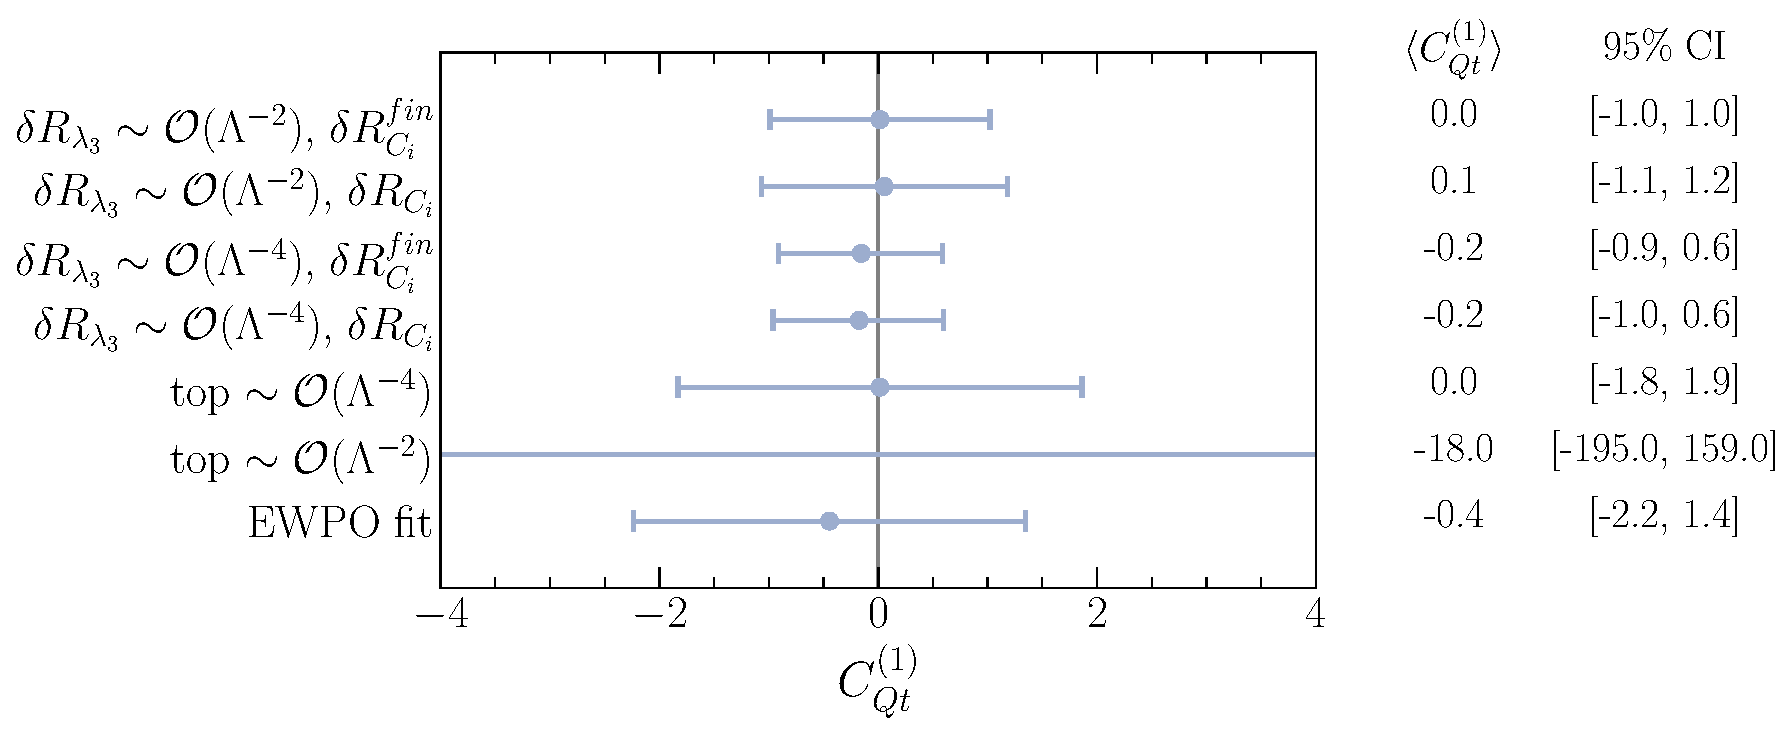
\includegraphics[width=0.75\linewidth]{fig/uebeblick_Cqt1}
		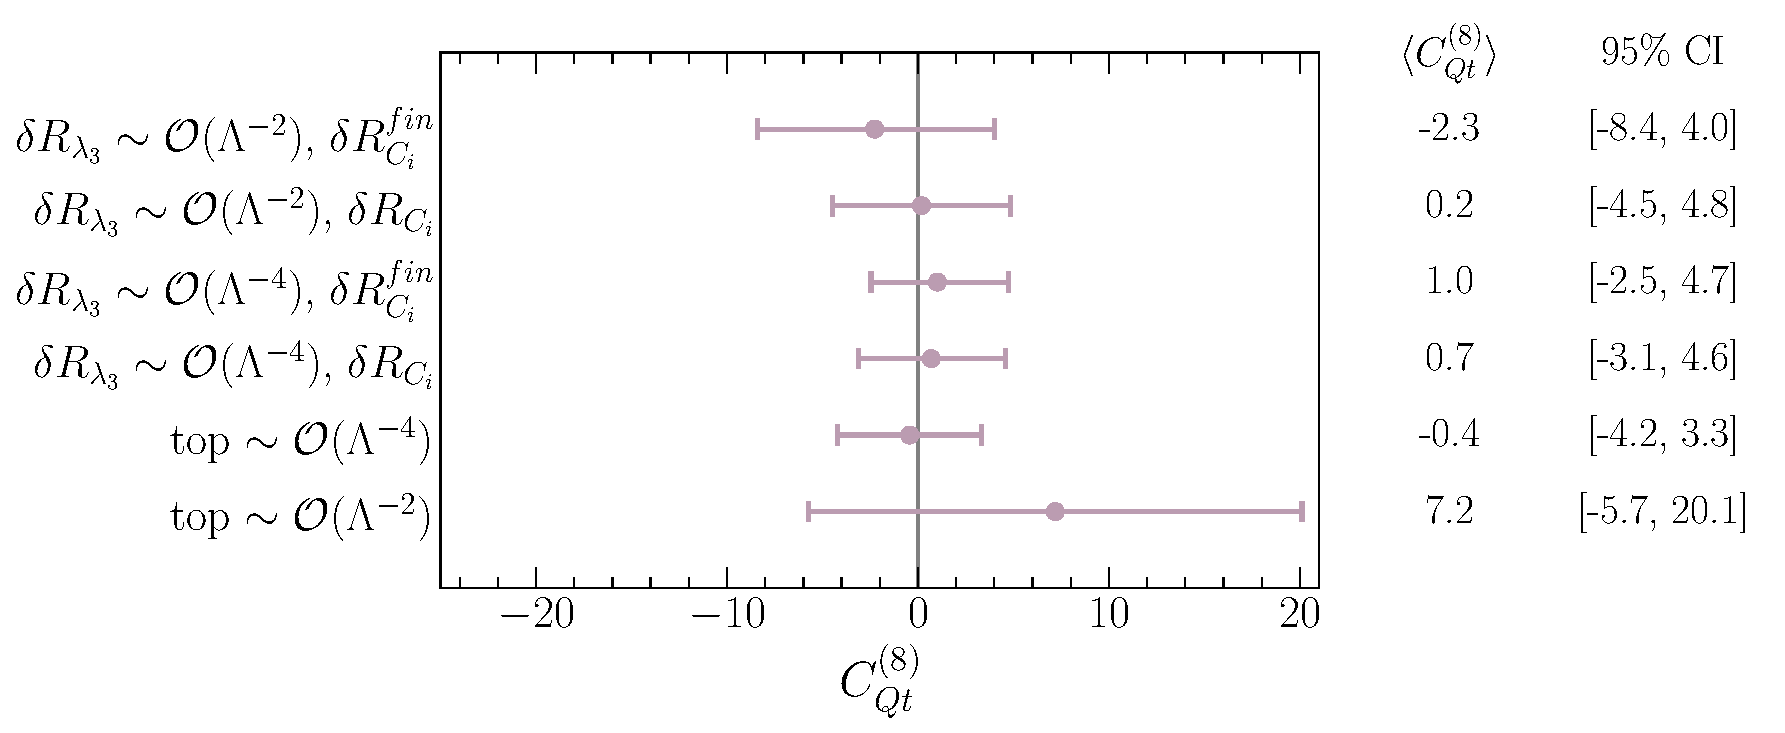
\includegraphics[width=0.75\linewidth]{fig/uebeblick_Cqt8} 
		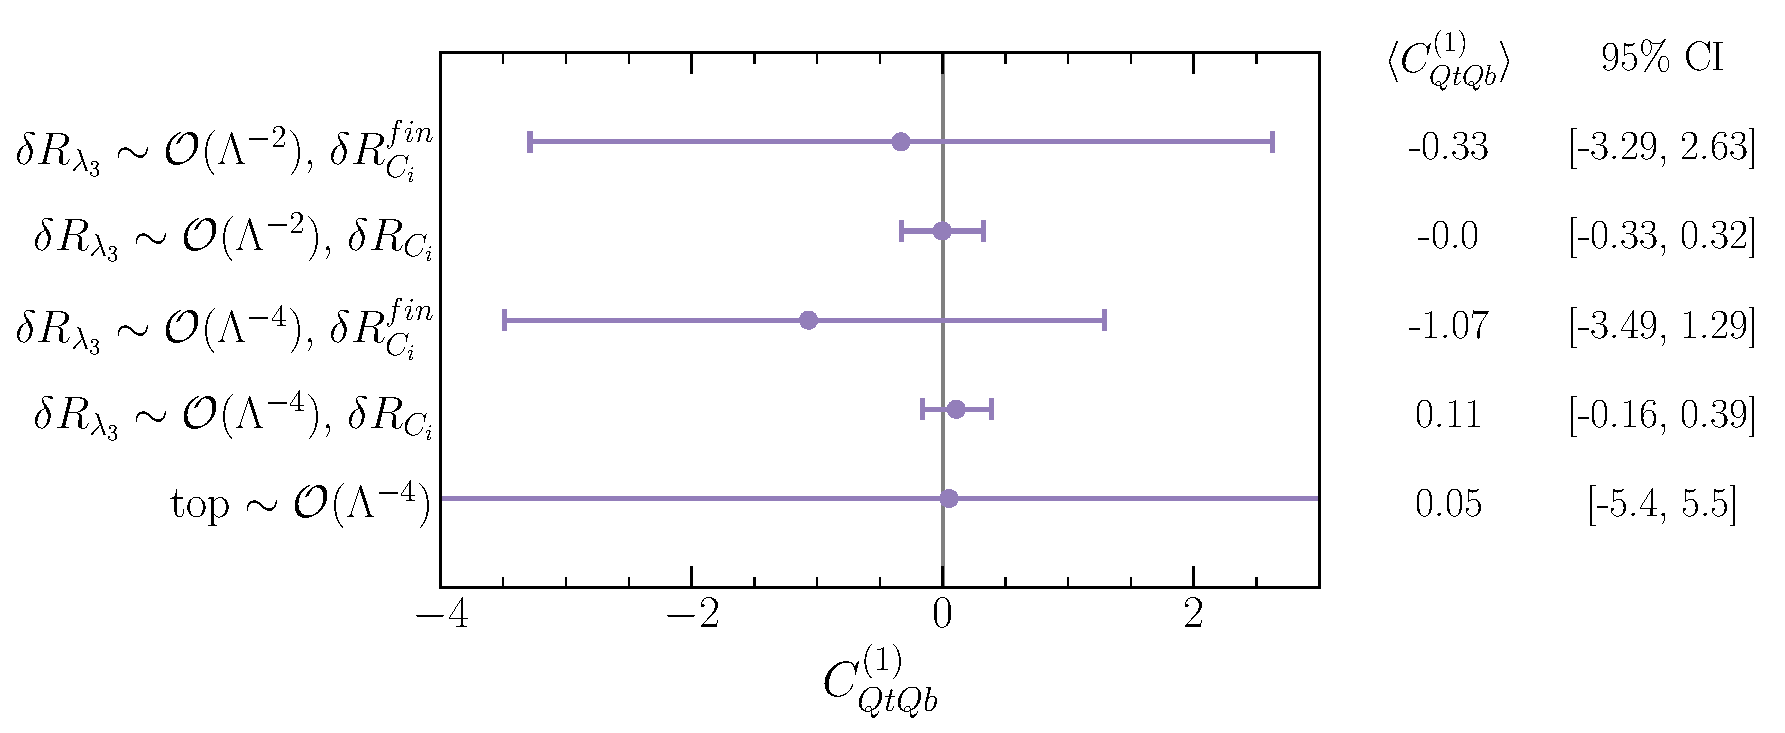
\includegraphics[width=0.75\linewidth]{fig/uebeblick_Cqtqb1}
		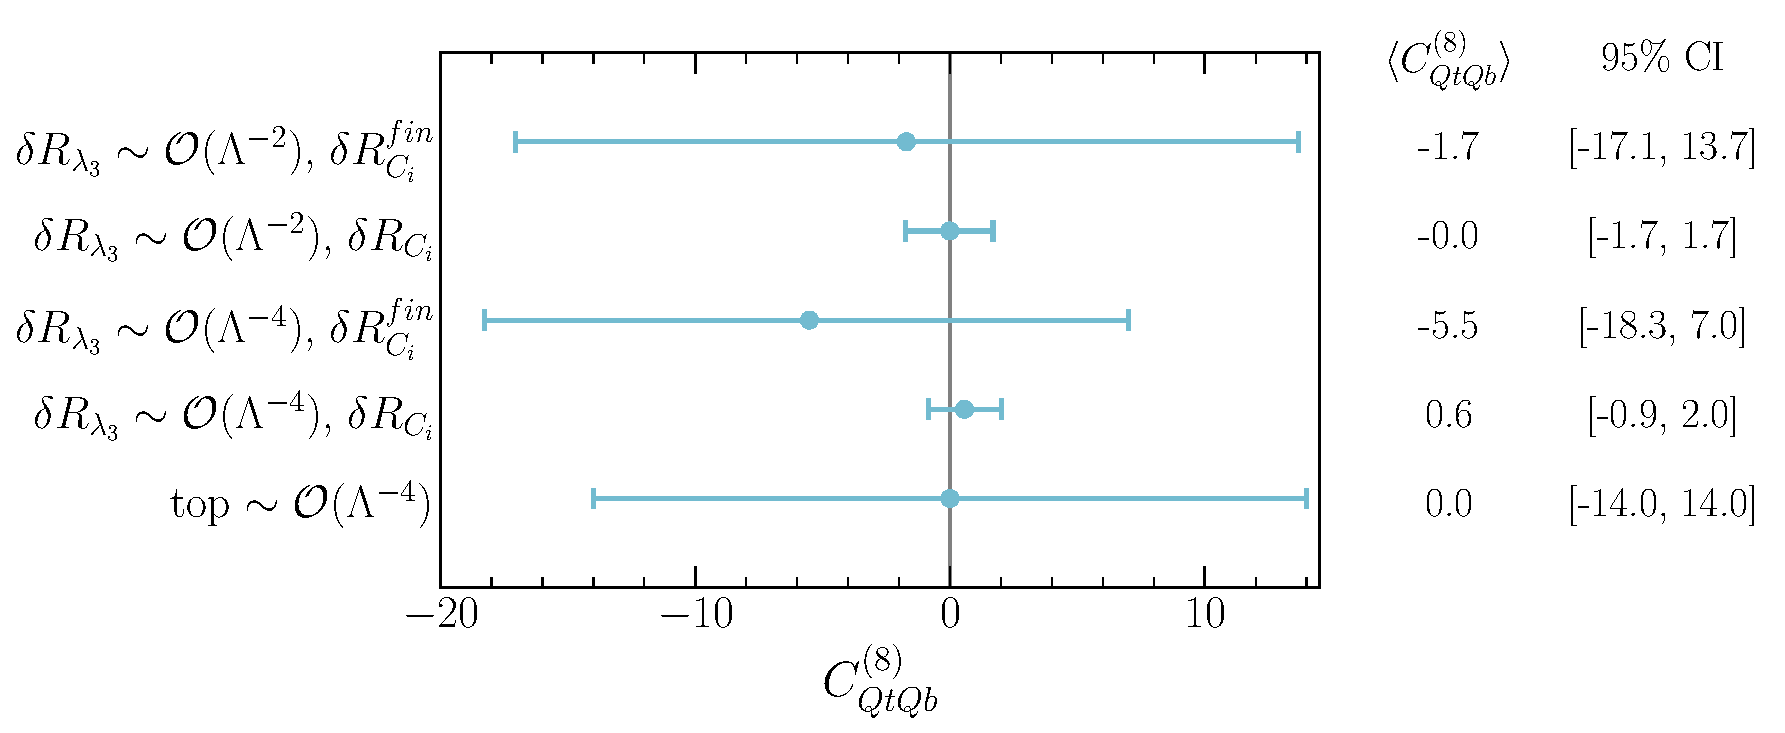
\includegraphics[width=0.75\linewidth]{fig/uebeblick_Cqtqb8}
	\end{center}
	\vspace*{-0.5cm}
	\caption{Forest plots illustrating the means and 95\% CIs of the posteriors built from the four-fermion Wilson coefficients with $C_\phi$ marginalised.  The plots confront also the truncation of the EFT at $\mathcal{O}(1/\Lambda^2)$ and $\mathcal{O}(1/\Lambda^4)$ of $\delta R_{\lambda_3}$ as defined in \eqref{eq:degrassi}. The 95\% CI bounds stem from Higgs data. The last two rows for each operator show instead the limits obtained by a single parameter fit to top data, linear and quadratic. The top data results are taken from~\cite{Ethier:2021bye} for $C_{Qt}^{(1),(8)}$ and~\cite{Hartland:2019bjb} for $C_{QtQb}^{(1),(8)}$. }
		\label{fig:summ4f}
\end{figure}
In \autoref{fig:summ4f} we show the limits of a two-parameter fit for various heavy quark Wilson coefficients $C_{i}$, marginalising over $C_\phi$. 
We confront them also with the limits obtained from fits to top data \cite{Ethier:2021bye, Ellis:2020unq, Hartland:2019bjb, Brivio:2019ius,DHondt:2018cww, Zhang:2017mls}. 
Note that, although our bounds do not come from a global fit, they can be compared with similar results from the the fits to top data that assume that
only one operator is ``switched on'' at a time.
In these cases, we find that our new bounds are more stringent or at least comparable to the 95\% CI bounds on the  $C_{i}$ operators fit results from top data. We also note that, while the limits from top data show a large uncertainty from the EFT truncation\footnote{In particular, for the $C_{QtQb}^{(1),(8)}$ operator the references only calculate contributions of order $\mathcal{O}(1/\Lambda^4)$. (The fit considering only linear terms would result in bounds of order  $\mathcal{O}(10^4)$.) Hence, in this case, we only quote the quadratic bounds.}, even when only one operator is considered at a time, our NLO results for the four-quark operators are quite stable if one considers quadratic effects, as mentioned above. 
On the other hand, fig.~\ref{fig:summ4f} also shows that there is a rather large uncertainty associated to the EFT truncation of the effects of the $\mathcal{O}_{\phi}$ operator in the wave function renormalization of the Higgs boson. Furthermore, the plot diplays the bounds for two different assumptions for the scale at which the operators are defined. The lines showing $\delta R^{fin}$ assume that there are only the corresponding four-quark operator and $\mathcal{O}_{\phi}$ at the electroweak scale\footnote{We neglect in this case the small running between the scales involved in the different processes included in the fit.}, while the line corresponding to $\delta R$ shows the limits assuming that the four-fermion operators (and $\mathcal{O}_{\phi}$) are the only ones at a scale $\Lambda=1\text{ TeV}$. 
We can again infere from the fact that the bounds remain the same order of magnitude between $\delta R^{fin}$ and $\delta R$ that the inclusion of the finite terms for the operators $\mathcal{O}_{Qt}^{(1),(8)}$ is important if the new physics scale is not extremely high. Instead, for the operators $\mathcal{O}_{QtQb}^{(1),(8)}$ the bounds become much stronger when including the logarithmic piece, so we can conclude that in that case the finite piece is less relevant.
In all the fit results that we will present in what follows, we will assume that the Wilson coefficients are always evaluated at the scale $\Lambda=1$ TeV.

In \autoref{fig:summcphi} we show the limits on $C_\phi$ for various two-parameter fits including the two different EFT truncations of $\delta R_{\lambda_3}$. 
We also show the results from a single parameter fit on $C_{\phi}$. 
For comparison, we show the ATLAS limits from full LHC run-II Higgs pair production in the final state~$b\bar{b} \gamma \gamma$~\cite{ATLAS:2021jki} where we have translated the bounds from $\kappa_\lambda\equiv\lambda_3/\lambda_3^{\SM}$ to the SMEFT, keeping both linear and quadratic terms.  While the limits on $C_{\phi}$ from single and double Higgs production are of similar size when keeping terms up to $\mathcal{O}(1/\Lambda^4)$ in the single Higgs fit, the limits from single Higgs become weaker if one keeps only terms up to $\mathcal{O}(1/\Lambda^2)$.  In this case, the fit remains questionable leading to limits beyond the perturbative unitarity bound of ref.~\cite{DiLuzio:2017tfn}. Instead, for Higgs pair production  is makes only a negligible effect  if linear or up to quadratic terms in the EFT expansion are kept  for the $C_\phi>0$ bound, while the bound weakens at linear order in $1/\Lambda^2$ for $C_\phi<0$~\cite{IML}.  We also see that the limits on $C_{\phi}$ become significantly weaker in a two-parameter fit with the four-quark operators, indicating that in a proper global SMEFT fit also the loop effects of other weakly constrained operators, such as these, need to be accounted for. 
\begin{figure}[t!]
	\begin{center}
		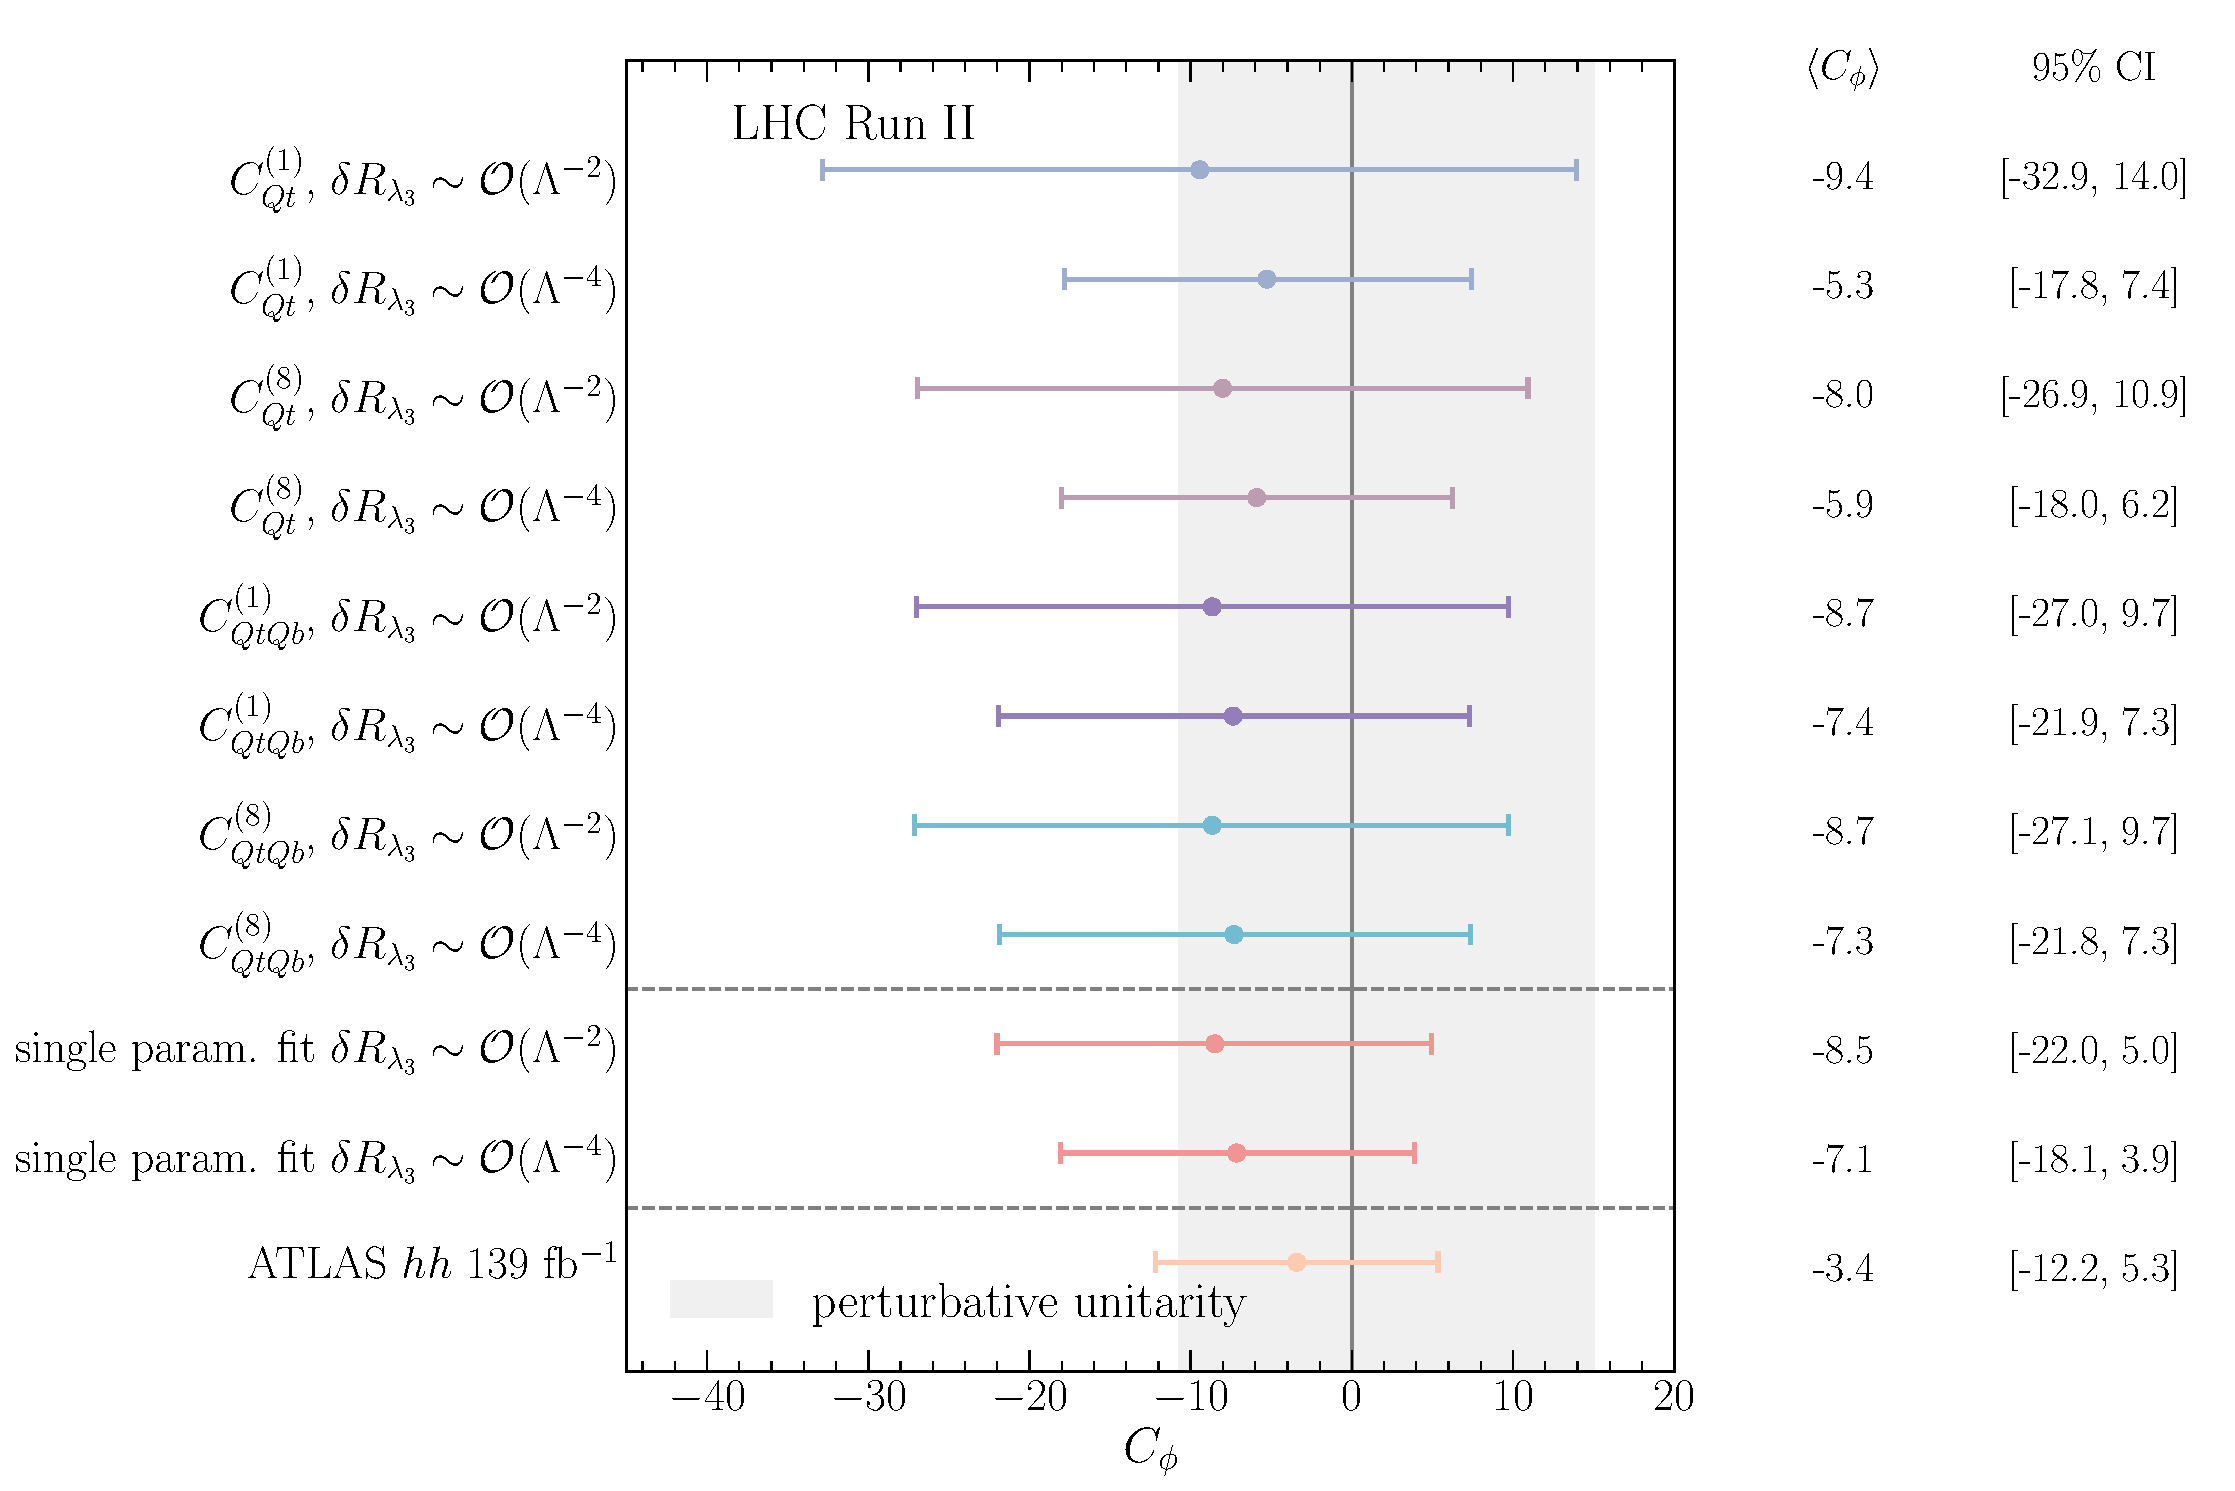
\includegraphics[width=\linewidth]{fig/uebeblick_forest_cphi_LHC_RunII}
	\end{center}
	\caption{A forest plot illustrating the means and 95\% CIs of the posteriors built from the  $C_\phi$  in a two-parameter fit with the four-fermion operators marginalised. We compare the fit results for $C_\phi$ from full run-II Higgs data keeping terms up to $\mathcal{O}(1/\Lambda^2)$ or $\mathcal{O}(1/\Lambda^4)$ in $\delta R_{\lambda_3}$.  For comparison, also the 95\% CI and means for the single parameter fit for $C_\phi$ with the same single Higgs data is shown as well as the bounds on $C_{\phi}$ from the $139$ fb$^{-1}$ search for Higgs pair production~\cite{ATLAS:2021jki}. The horizontal grey band illustrates the perturbative unitarity bound~\cite{DiLuzio:2017tfn}. \label{fig:summcphi}  }
\end{figure}
 %%%%%%%%%%%%%%%%%%%
\subsection{Two parameter fits \label{App:fitplots}}
%%%%%%%%%%%%%%%%%%%

We present in figs.~\ref{2param-cqt} and~\ref{2param-cqtqb} the $68\%$ and $ 95\%$  highest posterior density contours of the two-parameter posterior distributions and their marginalisation for the two-parameter fits involving $C_\phi$ and one of the four-heavy quark Wilson coefficients, evaluated at the scale $\Lambda=1$ TeV.  
Both linearised and quadratically truncated $\delta R_{\lambda_3}$ fits are shown, and we observe that the $95\%$ CI bounds (shown on top of the panels) and correlations depends on the truncation.

\begin{figure}[h!]
	\begin{center}
		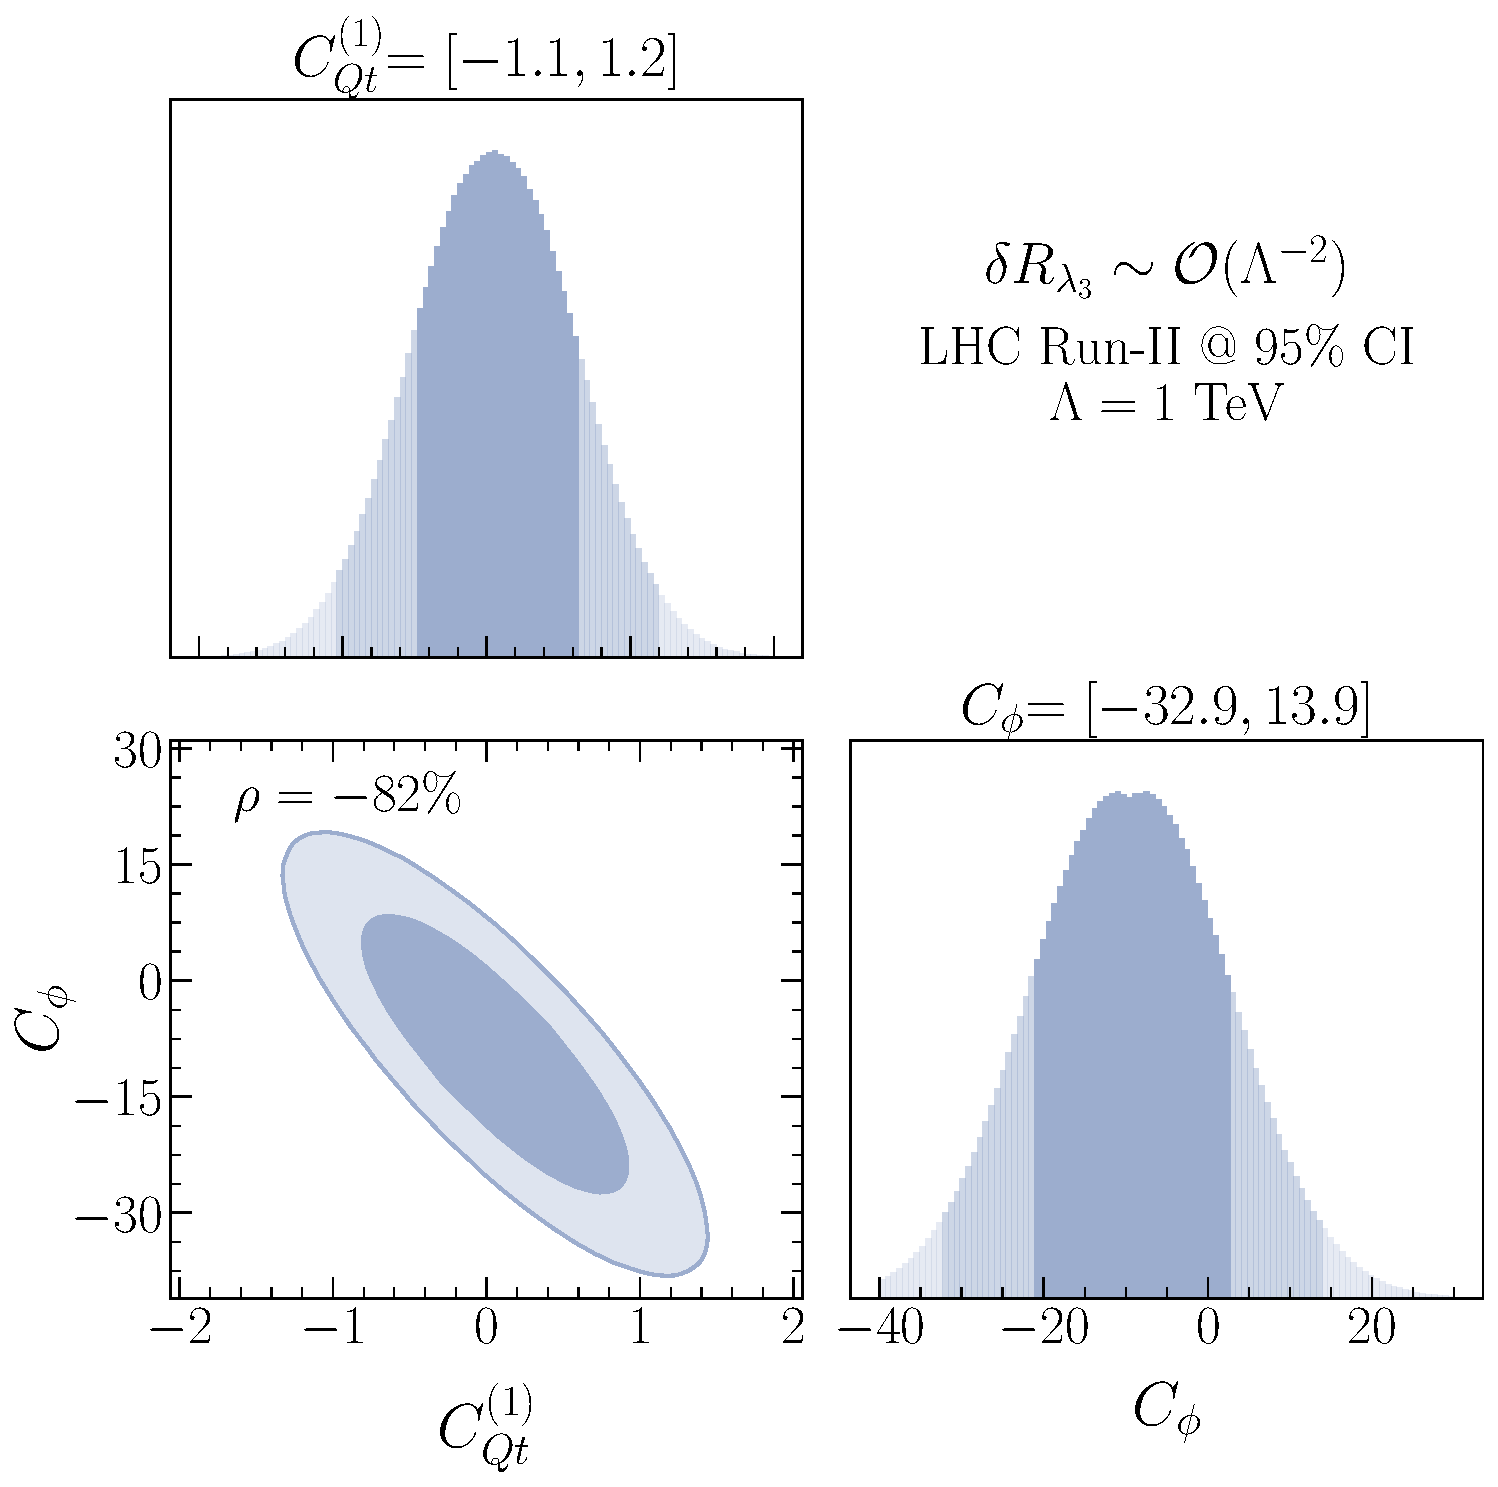
\includegraphics[width=0.45\linewidth]{fig/Cqt1_LHC_RunII_linearl3_rge}
		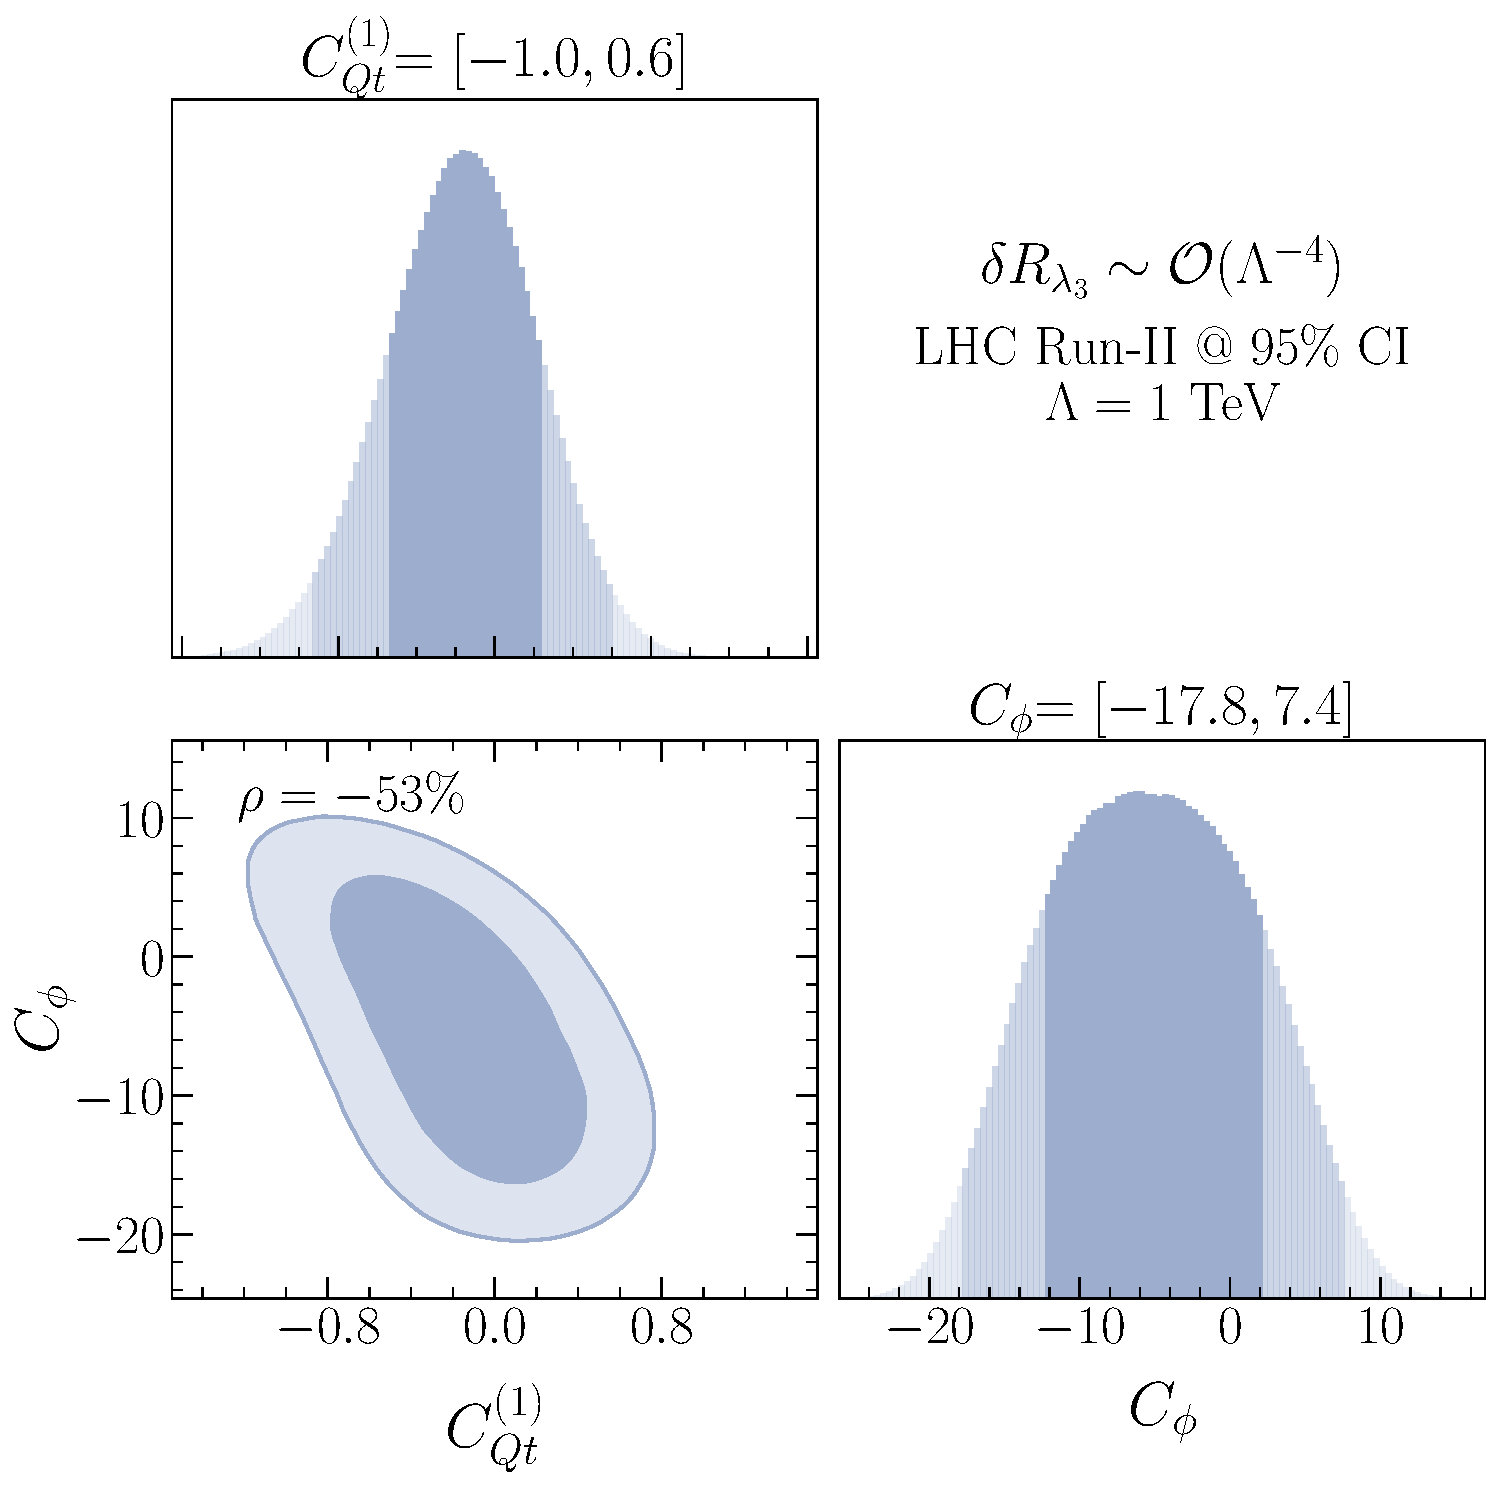
\includegraphics[width=0.45\linewidth]{fig/Cqt1_LHC_RunII_quadl3_rge} \\ 
		\includegraphics[width=0.45\linewidth]{fig/Cqt8_LHC_RunII_linearl3_rge}
		\includegraphics[width=0.45\linewidth]{fig/Cqt8_LHC_RunII_quadl3_rge} 
	\end{center}
	\caption{The 68\% and 95\% highest density posterior contours of the posterior distribution of $C_\phi$ with $C_{Qt}^{(1)}$ (up) and $C_\phi$ with $C_{Qt}^{(8)}$ (down) with the marginalised one-dimensional posteriors for each of the Wilson coefficients and their 68\% and 95\% HDPIs (shown above in numbers the 95\% CI bounds). 
		The limits correspond to values of the Wilson coefficients evaluated at the scale $\Lambda=1$ TeV.
		On the left we used the linear scheme in $\delta R_{\lambda_3}$ while on the right we keep up to quadratic terms in   $\delta R_{\lambda_3}$. \label{2param-cqt} } 
\end{figure}

\begin{figure}[h!]
	\begin{center}
		\includegraphics[width=0.45\linewidth]{fig/Cqtqb1_LHC_RunII_linearl3_rge}
		\includegraphics[width=0.45\linewidth]{fig/Cqtqb1_LHC_RunII_quadl3_rge} \\ 
		\includegraphics[width=0.45\linewidth]{fig/Cqtqb8_LHC_RunII_linearl3_rge}
		\includegraphics[width=0.45\linewidth]{fig/Cqtqb8_LHC_RunII_quadl3_rge} 
	\end{center}
	\caption{The 68\% and 95\% highest density posterior contours of the posterior distribution of $C_\phi$ with $C_{QtQb}^{(1)}$ (up) and $C_\phi$ with $C_{QtQb}^{(8)}$ (down) with the marginalised one-dimensional posteriors for each of the Wilson coefficients. and their 68\% and 95\% HDPIs (shown above in numbers the 95\% CI bounds). 
		The limits correspond to values of the Wilson coefficients evaluated at the scale $\Lambda=1$ TeV. 
		Similar to $C_{Qt}^{(1),(8)}$, the left plot shows the linearised  $\delta R_{\lambda_3}$ while the right one shows the quadratic scheme in the trilinear Higgs self-coupling modification. Due to the degeneracy between these Wilson coefficients the posterior contours and their marginalised intervals look very similar for both of them (except for the range they cover).  \label{2param-cqtqb} }
\end{figure}
%%%%%%%%%%%%%%%%%%%
One of the important aspects of multivariate studies is the correlation among variables. Apart from the two-parameter fits discussed above, here we also consider a four-parameter fit to $C_\phi$ plus the three directions in the four heavy-quark operator parameter space that the Higgs rates are
mostly sensitive too, i.e. neglecting $C_{QQ}^{(1),(3) }$ and $C_{tt}$, and trading $C_{QtQb}^{(1)}$ and $C_{QtQb}^{(8)}$ by $C_{QtQb}^{+}$.
%%%%%%%%%%
\begin{figure}[t!]
	\begin{center}
	%	\vspace{-1.5cm}
		\includegraphics[width=.6\linewidth]{fig/4param_fit_LHC_RunII_l3L_rge}\\
		%
		\includegraphics[width=.6\linewidth]{fig/4param_fit_LHC_RunII_l3Q_rge}
	%	\vspace{-.5cm}
	\end{center}
	\caption{The marginalised 68\% and 95\% HDPI's for the four-parameter fits including the different four-quark Wilson coefficients and $C_\phi$. The numbers above the plots show the 95\% CI bounds while the correlations are given on the top-right side. 
		These limits correspond to values of the Wilson coefficients evaluated at the scale $\Lambda=1$ TeV. 
		The upper panel shows the fit including up to $\mathcal{O}(1/\Lambda^2)$ in $\delta R_{\lambda_3}$  while the lower one shows the fit with including also  $\mathcal{O}(1/\Lambda^4)$.  \label{fig:4param} }
\end{figure}
%
When considering two- or four-parameter fits of $C_\phi$ and the four-heavy-quark Wilson coefficients, we observe a non-trivial correlation patterns amongst these coefficients.  Figure~\ref{fig:4param} illustrates these correlation patterns clearly for the four-parameter fit. 
We observe that the Wilson coefficients $C_{Qt}^{(1),(8) }$ are strongly correlated because, in analogy to $C_{QtQb}^{(1),(8) }$, they only appear in  certain linear combination whenever correcting the Yukawa coupling. However,  unlike $C_{QtQb}^{(1),(8) }$ they are not completely degenerate because the main part of the NLO correction to $t\bar t h$ does not contain the aforementioned linear combination.  The four-parameter fit also reveals that the Wilson coefficients~$C_{Qt}^{(1),(8) }$ have a large correlation with ~$C_{QtQb}^{+}$ because all of the four Wilson coefficients appear in a linear combination in the NLO corrections except for $ h\to b\bar b$ and $ t\bar{t} h$. However, this correlation is not as strong due to the large NLO correction of the Higgs decay $h \to b \bar b$ from ~$C_{QtQb}^{(1),(8) }$. Moreover, the correlation between the four-heavy-quark Wilson coefficients  and $C_{\phi}$ depends on the $\delta R_{\lambda_3}$ truncation. In Appendix~\ref{App:fitplots}  we present similar correlation plots for various two-parameter fits, where the same behaviour of the change in the correlation with the inclusion of quadratic terms ~$\delta R_{\lambda_3}$ is found. The correlation in those cases are though generally stronger.
%%%%%%%%%%%%
\subsection{Prospects for HL-LHC}
\begin{figure}[t!]
	\begin{center}
		\includegraphics[width=0.75\linewidth]{fig/uebeblick_forest_ci}
	\end{center}
	\caption{ Results of a single parameter fit showing the improvement in constraining power of the HL-LHC over the current bounds from Run-2 data. The limits correspond to values of the Wilson coefficients evaluated at the scale $\Lambda=1$ TeV. \label{fig:HLLHC} }
\end{figure}

\begin{figure}
	\begin{center}
		\includegraphics[width=0.75\linewidth]{fig/uebeblick_forest_cphi_singleparam}
	\end{center}
	\caption{A forest plot illustrating the means and 95\% CIs of the posteriors built from the  $C_\phi$  in a single-parameter fit, showing also the differences in including terms of $\mathcal{O}(1/\Lambda^2)$ or up to $\mathcal{O}(1/\Lambda^4)$ in the definition of $\delta R_{\lambda_3}$. For comparison, also the limits and projections from searches for Higgs pair production are shown.  \label{fig:summcphihl-lhc}  }
\end{figure}
We now turn to examine the potential of the HL-LHC. For this, we use the CMS projections for the single Higgs signal strengths provided in refs.~\cite{CMS-PAS-FTR-18-011,twiki} for a centre-of-mass energy of $\sqrt{s}=14$ TeV and integrated luminosity of $ 3\, \mathrm{ab}^{-1}$. We use the projections for the S2 scenario explained in~\cite{Cepeda:2019klc}. These assume the improvement on the systematics that is expected to be attained by the end of the HL-LHC physics programme, and that theory uncertainties are improved by a factor of two with respect to current values. 
These projections are assumed to have their central values in the SM prediction with the total uncertainties summarised in table~\ref{table:resHiggsExp} in Appendix~\ref{App:numinput}.\footnote{The correlation matrix for the S2 scenario can be found on the webpage~\cite{twiki}.} 

In \autoref{fig:HLLHC} we confront the results of the fits to Run-2 data with the projections for the HL-LHC for single parameter fits. For the operators $\mathcal{O}_{Qt}^{(1),(8)}$ the constraining power of the HL-LHC is roughly a factor two better as the current bounds we could set from single Higgs data, while for the operators $\mathcal{O}_{QtQb}^{(1),(8)}$ the improvement is a little less.
In \autoref{fig:summcphihl-lhc} we show the limits on $C_{\phi}$ in a single parameter fit for Run-2 and the projections for the HL-LHC
including in $\delta R_{\lambda_3}$ up to order $\mathcal{O}(1/\Lambda^2)$ or $\mathcal{O}(1/\Lambda^4)$. While for Run-2 data the inclusion of $\mathcal{O}(1/\Lambda^4)$ made a huge difference, this is less pronounced for the HL-LHC projections. Our results are very similar to the projections presented in a $\kappa_{\lambda}$ fit in \cite{DiMicco:2019ngk}. 
We confront this also with data from searches for Higgs pair production $139$ fb$^{-1}$ \cite{ATLAS:2021jki}  and HL-LHC projections~\cite{CMS:2018ccd} on Higgs pair production, showing that Higgs pair production will still allow to set stronger limits on $C_{\phi}$. 


%%%%%%%%%%%%%%%%%%%%%%%%%%%%%%
\section{Summary and discussion \label{sec:conc}}
%%%%%%%%%%%%%%%%%%%%%%%%%%%%%%

In this paper, we have computed the NLO corrections induced by third generation four-quark operators in Higgs observables that are relevant for its production and decay at the LHC. 
Our results show that such processes are sensitive to the all possible chiral structures for the third generation four-quark operators in the dimension-six SMEFT, but in different degrees. 
Operators with different chiralities are, for instance, the only ones that can contribute to Higgs production via gluon fusion, and the decay of the Higgs boson to gluons, photons and bottom quarks pairs.  The latter are particularly sensitive to the top-bottom operators $\mathcal{O}_{QtQb}^{(1),(8)}$, which then also significantly affect the total decay width. In the associate production of a Higgs boson with a top quark pair, on the other hand, all the third generation four-fermion operators enter.
Sensitivity to four-quark operators where all fields have the same chirality, however, is only possible for large values of the Wilson coefficients, in a way that they can generate contributions beyond the size of current theory uncertainties. 
%
\begin{figure}
	\begin{center}
		\includegraphics[width=0.75\linewidth]{figures/SMEFT_collection}
	\end{center}
	\caption{A forest plot illustrating the means and 95\% CIs of the posteriors built from the  $C_\phi$  in a single-parameter fit, showing also the differences in including terms of $\mathcal{O}(1/\Lambda^2)$ or up to $\mathcal{O}(1/\Lambda^4)$ in the definition of $\delta R_{\lambda_3}$. For comparison, also the limits and projections from searches for Higgs pair production are shown.  \label{fig:summcphihl-lhc}  }
\end{figure}
The $t\bar{t}h$ process is also rather important in setting limits on the four-quark operators $\mathcal{O}_{Qt}^{(1)}$ and $\mathcal{O}_{Qt}^{(8)}$, due to the comparatively large NLO corrections they induce in this process with respect to others. It also breaks a degeneracy among the Wilson coefficients of those two operators, which always appear in a single combination for all other processes. 
\par
To illustrate the constraining power of single Higgs processes in bounding these four-quark operators, we performed several simplified fits to these interactions and find that the resulting limits from our fits are, in some cases, comparable or better than similar results obtained from top data \cite{Ethier:2021bye, Hartland:2019bjb}.
\par
We have also performed a combined fit including the above-mentioned four-quark operators and the operator $\left(\phi^\dagger \phi\right)^3$, that modifies the Higgs potential and the trilinear Higgs self-coupling. Due to the lack of powerful constraints from top data, the inclusion of the four-fermion operators diminishes the power of setting limits on the trilinear Higgs self-coupling
from single Higgs observables. 
From our analysis we conclude that, in the absence of strong direct bounds on the third-generation four-quark operators, these should be included into a global fit on Higgs data, when attempting to obtain model-independent bounds on the trilinear Higgs self-coupling. The results of our calculations are presented such that they can be easily used by the reader in truly global fits including all other interactions entering at the LO. 
We leave this, as well as the inclusion of differential Higgs data, to future work.
%

Finally, we also illustrated the increase in constraining power expected during the high-luminosity phase of the LHC by presenting the HL-LHC projections of the above-mentioned fits.  

Moving beyond hadron colliders, it must be noted that the interplay between the Higgs trilinear and four heavy-quark operators in Higgs processes is expected to be less of an issue at future leptonic Higgs factories, such as the FCC-ee~\cite{FCC:2018byv,FCC:2018evy}, ILC~\cite{Bambade:2019fyw,LCCPhysicsWorkingGroup:2019fvj}, CEPC~\cite{An:2018dwb,CEPCStudyGroup:2018ghi} or CLIC~\cite{CLICdp:2018cto,deBlas:2018mhx}. At these machines, the effects of $C_\phi$ are still ``entangled'' with those
of the four-fermion operators in the Higgs rates, but only through the decay process, i.e. via the contributions to the BRs. However, Higgs production is purely electroweak, namely via Higgs-strahlung ($Zh$: $e^+ e^- \to Zh$) or $W$ boson fusion, and receives no contributions from the four-quark operators at the same order in perturbation theory where $C_\phi$ modifies these processes, i.e. NLO. 
Moreover, at any of these future $e^+ e^-$ Higgs factories there is the possibility of obtaining a sub-percent determination of the total $Zh$ cross section at $e^+ e^-$ colliders, by looking at events recoiling against the $Z$ decay products with a recoil mass around $m_h$. This observable is therefore completely insensitive to the four-quark operators, while still receiving NLO corrections from $C_\phi$. 
Although, in practice, in a global fit one needs to use data from all the various Higgs rates at two different energies to constrain all possible couplings entering at LO in the Higgs processes and also obtain a precise determination of $C_\phi$ ~\cite{DiVita:2017vrr}, the previous reasons should facilitate the interpretation of the single-Higgs bounds on the Higgs self-coupling at $e^+e^-$ machines.

We conclude this paper with a few words on the relevance of the results presented here when interpreted from the point of view of specific models of new physics. 
In particular, one important question is \textit{ are there models where one expects large contributions to four-top operators while all other interactions entering in Higgs processes are kept small?}
%
Indeed, large contributions to four-top operators can be expected in various BSM scenarios.\footnote{Generically, models where four-top interactions are much larger than four-fermion operators of the first and second generation can be easily conceived from some UV dynamics coupling mostly to the third generation of quarks hence respecting the Yukawa hierarchies.} For instance, in Composite Higgs Models, in which the top quark couples to the strong dynamics by partial compositeness, one expects on dimensional grounds that some of the four-top quark operators are of order $1/f^2$, where $f$ indicates the scale of strong dynamics \cite{Banelli:2020iau}. 
By its own nature, however, Composite Higgs models also predict sizeable contributions to the single Higgs couplings $\sim 1/f^2$. While, in general, sizeable modifications of the Higgs interactions are typically expected in scenarios motivated by ``naturalness'', this is not necessarily the case in other scenarios. 
It is indeed possible to think of simple models where modifications of the Higgs self-interactions or contributions to four-quark operators are the only corrections induced by the dimension-six interactions at tree level, see~\cite{deBlas:2017xtg}.
Thinking, for instance, in terms of scalar extensions of the SM, there are several types of colored scalars whose tree-level effects at low energies can be represented by four-quark operators only, e.g. for complex scalars in the $(6,1)_{\frac 1 3}$ and $(8,2)_{\frac 1 2}$ SM representations ($\Omega_1$ and $\Phi$ in the notation of \cite{deBlas:2017xtg}).  If these colored states are the only moderately heavy new particles, our results can provide another handle to constrain such extensions. 
One must be careful, though, as a consistent interpretation of our results for any such models would require to include higher-order corrections in the matching to the SMEFT. At that level, as shown e.g. by the recent results in \cite{Anisha:2021hgc}, multiple contributions that modify Higgs processes at LO are generated at the one-loop level, and are therefore equally important as the NLO effects of the (tree-level) generated four-quark operators.\footnote{Furthermore, given that some SMEFT interactions induce tree-level contributions to Higgs processes that in the SM are generated at the loop level, e.g. ${\cal O}_{\phi G}$ in gluon fusion, a consistent interpretation in terms of new physics models may require to include up to two-loop effects in the matching for such operators, for which there are currently no results or tools available.}
%
In any case, one must note that, even if similar size contributions to single Higgs processes are generated, the four-top or Higgs trilinear effects can provide extra information on the model.
%
For instance, in some of the most common scalar extensions of the SM, with an extra Higgs doublet, $\varphi\sim (1,2)_{\frac 12}$, tree-level contributions to some of the four-heavy-quark operators discussed in this paper are generated together with modifications on the Higgs trilinear self-coupling.
These two effects are independent but they are both correlated with the, also tree level, modifications of the single Higgs couplings. Essentially, the LO effects on Higgs observables are proportional to $\lambda_\varphi y_\varphi^f$, where $\lambda_\varphi $ is the scalar interaction strength of the $(\varphi^\dagger \phi)(\phi^\dagger \phi)$ operator and $y_\varphi^f$ the new scalar Yukawa interaction strength, whereas the NLO effects are proportional to the square of each separate coupling. Hence, these effects might help to resolve (even if only weakly) the flat directions in the model parameter space that would appear in a LO global fit.
%
At the end of the day, for a proper interpretation of the SMEFT results in terms of the widest possible class of BSM models, all the above simply remind us of the importance of being global in SMEFT analyses, to which our work contributes by including effects in Higgs physics that enter at the same order in perturbation theory as modifications of the Higgs self-coupling.

        %!TEX encoding = UTF-8 Unicode
% !TeX spellcheck = en_GB
%%%%%%%%%%%%%%%%%%%%%%%%%%%%%%%%%%%%%%
\chapter{ Associated $Zh$ production via gluon fusion at NLO }\label{chap:hz}
%%%%%%%%%%%%%%%%%%%%%%%%%%%%%%%%%%%%%%
\section{Overview}
\par As we have seen in the previous sections, Higgs couplings to the weak vector bosons, i.e. $Z$ and $W$ is approaching the precision level. Moreover, the associated Higgs production with these bosons is the first channel used to observer the Higgs decaying into beauty quarks   $h \rightarrow b \bar{b}$ by both ATLAS and CMS~\cite{Aaboud:2018zhk, Sirunyan:2018kst}. Hence, the $ Vh$ Higgs production channel is one of the important channels to look for in the future runs of the LHC for better measurement of the $VVh$ coupling as well as Higgs coupling to the beauty quark. As the statistical and systematic uncertainties coming from the experimental setup of the LHC get reduced in the future runs, due to higher integrated luminosity and uprated detectors and analysis techniques. There is a  need to reduce theoretical uncertainties emerging from the perturbative calculations of  cross-sections. In order to achieve that, one should include more terms in the perturbative expansion in the couplings, particularly the string coupling $\alpha_s$. In this chapter, we are interested in the channel $pp\to Zh$, which is quark-initiated tree-level process at LO interpreted as \textbf{Drell-Yan process}~ \cite{Han:1991ia,Brein:2003wg}. This process has been computed up to next-to-next-to-leading-order (NNLO) in QCD ($\sim \alpha_s^2$), and
at next-to-leading-order (NLO) in the EW interactions ($\sim \alpha^2 $) \cite{Amoroso:2020lgh}.
%%
\par Despite arising for the first time at NNLO in perturbation theory to the partonic cross-section  , the gluon fusion channel $g g \rightarrow Zh$ has a non-negligible contribution to the hadronic cross-section of  $pp\to Zh$ process, which could reach $>16\%$ of the total cross-section contribution at $14$ TeV~\cite{Cepeda:2019klc}.The contribution becomes more significant when looking at large invariant mass bins in the differential cross-section. This is due to the significant abundance of gluons at the LHC for large $Q$ as well as the top quark initiated contribution near the $t\bar t$ threshold~\cite{Englert:2013vua}.  The gluon fusion channel has a higher scales uncertainties than the quark induced one, and due to the significant contribution of the former, and the absence of gluon fusion channel for $Wh$ channel, the $Zh$ channel has  higher theoretical uncertainties. This motivates NLO calculation of the  $g g \rightarrow Z h$ channel in order to reduce these uncertainties and facilitate the precision measurement potential of the $Zh$ channel at the future LHC runs, such as sign and magnitude
of the top Yukawa coupling,  dipole operators \cite{Englert:2016hvy}
and it can receive additional contributions from new particles \cite{Harlander:2013mla}. Therefore, better understanding of the SM prediction of the $Zh$ gluon fusion channel is crucial for both the SM precision measurements of Higgs production within the SM and for testing NP in this channel, e.g. new vector-like leptons.  
%%
\par  The leading order (LO) contribution to the $g g \rightarrow Z H$ amplitude, given by one-loop diagrams, was computed exactly in refs.\cite{Kniehl:1990iva, Dicus:1988yh}.However, for the NLO, the virtual corrections contain multi-scale two-loop integrals some of which are still not known analytically ( for the box diagram).  The fiirst computation of the NLO terms has been done by~\cite{Altenkamp:2012sx} using an asymptotic expansion in the limit
$\mt \rightarrow \infty$ and $m_b = 0$, and pointed to a $K$-factor of about $\sim2$.  Later, the computation has been improved via soft gluon resummation, and including NLL terms found in ref.\cite{Harlander:2014wda}, the NLL terms has been matched to the fixed NLO computation of~\cite{Altenkamp:2012sx}.  Top quark mass effects to the  $g g \rightarrow Zh$ process were first implemented using a combination of of large-$\mt$ expansion (LME) and Pad\'e approximants~\cite{Hasselhuhn:2016rqt}. 
%%%%%%%%%%%%%%%%%%%%%%%%%%%%%%%%%%%%%%%%%%%%%%%%%
 .  In addition, a data-driven method to extract
the non-Drell-Yan part of $p p \rightarrow Z H$, which is dominated by
the gluon-induced contribution, has been proposed in
ref.\cite{Harlander:2018yns}, exploiting the known relation between $W H$
and $ Z H$ associated production when only the Drell-Yan component of
the two processes is considered.  A qualitative study focusing on
patterns in the differential distribution has been conducted in
ref.\cite{Hespel:2015zea}, where $2 \rightarrow 2$ and $2 \rightarrow 3$
LO matrix elements were merged and matched to improve the description
of the kinematics.

Very recently, a new analytic computation  of the NLO virtual contribution
based on a high-energy expansion of the amplitude, supported by Pad\'e
approximants, and on an improved LME, has been
carried out \cite{Davies:2020drs}. The results are in agreement with a new
exact numerical study \cite{Chen:2020gae}, in the energy regions where the
expansions are legitimate. Nonetheless, an improvement on the analytic
calculation is still desirable, since the heavy-top and the
high-energy expansions do not cover well the region
$350\,  \si{\GeV} \lesssim \sqrt{\hat{s}} \lesssim 750\,  \si{\GeV}$, where
$\sqrt{\hat{s}}$ is the partonic center of mass energy. It should be
remarked  that this region provides a significant part of the hadronic cross
section at the LHC, about 68\%.

In this paper, we present an analytic calculation of the virtual NLO QCD
corrections to the $gg\to Z H$ process that covers the region
$\sqrt{\hat{s}} \lesssim 750\, \si{\GeV}$,  which contributes about 98\% to the hadronic
cross section. The most difficult parts, i.e.~the two-loop box
diagrams, are computed in
terms of a forward kinematics  \cite{Bonciani:2018omm} via an  expansion in
the $Z$ (or Higgs) 
transverse momentum, $\pt$, while the rest of the
virtual corrections is computed exactly. 
We remark that our calculation is complementary
to the results of ref.\cite{Davies:2020drs}, which covers the region of
large transverse momentum of the $Z$. Furthermore, the merging of the two
analyses
allows an analytic evaluation of the NLO virtual corrections in
$gg\to Z H$ in the entire phase space. 

\section{Definitions}
In this section we  introduce our definitions for the
calculation of the NLO QCD corrections to the associated production of
a Higgs and a $Z$ boson from gluon fusion.

The amplitude  $g^\mu_a(p_1)g^\nu_b(p_2)\to Z^\rho(p_3) H(p_4)$ can be written as
\bea
&&\amp=i \sqrt{2}\frac{\mz \Gfer \as(\mu_R)}{\pi}\delta_{ab}\epsilon^a_\mu(p_1)
\epsilon^b_\nu(p_2)\epsilon_\rho(p_3)\hat{\amp}^{\mu\nu\rho}(p_1,p_2,p_3 ),\\
&&\hat{\amp}^{\mu\nu\rho}(p_1,p_2,p_3 )=\sum_{i=1}^{6}
\mathcal{P}_i^{\mu\nu\rho}(p_1,p_2,p_3 )
\amp_i(\hat{s},\hat{t},\hat{u},\mt,\mh,\mz),
\label{eq:amp}
\eea
where $\Gfer$ is the Fermi constant, $\as(\mu_R)$ is the strong coupling
constant defined at a  scale $\mu_R$ and
$\epsilon^a_\mu(p_1)\epsilon^b_\nu(p_2)\epsilon_\rho(p_3)$ are the
polarization vectors of the gluons and the $Z$ boson, respectively. The
tensors $\mathcal{P}_i^{\mu\nu\rho}$ are a set of orthogonal
projectors, whose explicit expressions are presented in appendix \ref{app:uno}.
The corresponding form factors
$\amp_i(\hat{s},\hat{t},\hat{u},\mt,\mh,\mz)$ are functions of the
masses of the top quark ($\mt$), Higgs ($\mh$) and $Z$ ($\mz$) bosons, and of
the partonic Mandelstam variables
\beq
\hat{s}=(p_1+p_2)^2,~~ \hat{t}=(p_1+p_3)^2,~~ \hat{u}=(p_2+p_3)^2,
\eeq
where $\hat{s}+\hat{t}+\hat{u}=\mz^2+\mh^2$ and we took all the momenta to
be incoming.

The $\amp_i$ form factors can be expanded up to NLO terms as
\beq
\amp_{i} = \amp_i^{(0)} + \frac{\as}{\pi} \amp_i^{(1)}
\label{eq:ampexp}
\eeq
and the  Born partonic cross section can be written as
\beq
\hat{\sigma}^{(0)}(\hat{s})=
\frac{\mz^2 \Gfer^2 \as(\mu_R)^2}{64 \hat{s}^2(2\pi)^3}
\int^{\hat{t}^+}_{\hat{t}^-}d\hat{t}\sum_i \left|\amp_i^{(0)}\right|^2,
\eeq
where
$\hat{t}^\pm=[-\hat{s}+\mh^2+\mz^2\pm\sqrt{(\hat{s}-\mh^2-\mz^2)^2-4\mh^2\mz^2}\,]/2$.
\label{sec:due}

\begin{figure}
	\begin{center}
		\includegraphics[width=12cm]{./figures/Feynman_LO_und_NLO.eps}
		\caption{Examples of Feynman diagrams contributing to $gg \to ZH$ at  LO and
			NLO.}
		\label{fig:dia}
	\end{center}
\end{figure}

The Feynman diagrams that contribute to the $gg \to  ZH$ amplitude up to NLO
can be separated into triangle, box and double-triangle
contributions, the last type appearing for the first time at the
NLO level. Examples of LO (NLO) triangle and box
categories are shown in fig.\ref{fig:dia} $(a)$ - $(c)$
($(d)$ - $(f)$).
Due to the presence of a $\gamma_5$ in the axial coupling of the $Z$ boson to
the fermions in the loop, the projectors $\mathcal{P}_i^{\mu\nu\rho}$ are
proportional to the Levi-Civita total anti-symmetric tensor
$\epsilon^{\alpha\beta\gamma\delta}$ (see appendix \ref{app:uno}),
whose treatment in dimensional regularization is, as well known, delicate
and will be discussed in section \ref{sec:quattro}.

In our calculation we treat all the quarks but the top as massless.
As a consequence, the contribution to the amplitude of the first two generations
vanishes. Concerning the third generation, the contribution of the bottom
is present  in the triangle diagrams with the exchange of a $Z$ boson
(fig.\ref{fig:dia}$(b),(e)$) and in the double-triangle diagrams
(fig.\ref{fig:dia}$(g)$).
A nice observation in ref.\cite{Altenkamp:2012sx} allows to compute
easily the full (top+bottom) triangle contribution. As noticed in that
reference,
the triangle contribution with a $Z$ exchange contains a $ggZ^*$ subamplitude
which in the Landau gauge can be related to the decay of a massive vector boson
with mass $\sqrt{\hat{s}}$ into two massless ones, a process that is
forbidden by
the Landau-Yang theorem \cite{Landau:1948kw,Yang:1950rg}. As a consequence,
the full triangle contribution can be obtained from the top triangle diagrams
with the exchange of the unphysical scalar $G^0$, with the propagator of the
$G^0$ evaluated in the Landau gauge. This part of the top triangle
diagrams  can be obtained from the decay
amplitude of a pseudoscalar boson into two gluons which is  known in
the literature in the full mass dependence up to NLO terms \cite{Spira:1995rr,Aglietti:2006tp}. 

Given the above observation, our calculation of the NLO corrections to
the $gg \to ZH$ amplitude focuses on the analytic evaluation of the
double-triangle (fig.\ref{fig:dia}$(g)$) and two-loop box contributions
(fig.\ref{fig:dia}$(f)$). The former contribution is evaluated exactly.
The latter is evaluated via two different expansions: i) via  a LME, following
ref.\cite{Degrassi:2010eu}, up to and including ${\cal O}(1/\mt^6)$ terms,
which is expected to work below the $2\, \mt$ threshold; ii) via an expansion in
terms of the $Z$ transverse momentum, following ref.\cite{Bonciani:2018omm},
whose details are presented in the next section.

\section{Expansion in the transverse momentum}
\label{sec:tre}
The transverse momentum of the $Z$  boson can be written in
terms of the Mandelstam variables as
\beq
\pt^2=\frac{\hat{t}\hat{u}-\mz^2\mh^2}{\hat{s}}.
\label{ptdef}
\eeq
From  eq.(\ref{ptdef}), together with the relation between
the Mandelstam variables, one finds 
\beq
\pt^2+\frac{\mh^2+\mz^2}{2}\leq\frac{\hat{s}}{4}+\frac{\dm^2}{\hat{s}},
\label{ptexp}
\eeq
where
$\dm = (\mh^2 -\mz^2)/2$. Eq.(\ref{ptexp}) implies 
$\pt^2/\hat{s} < 1$ that, together with the kinematical constraints
$\mh^2/\hat{s}< 1$ and
$\mz^2/\hat{s} < 1$,  allows the expansion of the amplitude in terms of these
three ratios.


A direct expansion in $\pt$ is not possible at amplitude level, since $\pt$
itself does not appear in the amplitudes. However, as we argued in
ref.\cite{Bonciani:2018omm}, the expansion in $\pt^2/\hat{s}\ll 1$ is equivalent
to an expansion in terms of the ratio of the reduced Mandelstam variables
$t^\prime/s^\prime\ll 1$ or $u^\prime/s^\prime\ll 1$, depending whether we are
considering the process to be in a forward or backward kinematics. The
$s^\prime,\,t^\prime$ and $u^\prime$  variables are defined as
\beq
s^\prime=p_1\cdot p_2=\frac{\hat{s}}{2},~~
t^\prime=p_1\cdot p_3=\frac{\hat{t}-\mz^2}{2},~~ u^\prime =
p_2\cdot p_3=\frac{\hat{u}-\mz^2}{2}
\eeq
and satisfy
\beq
s^\prime + t^\prime + u^\prime =\dm.
\eeq

The cross section of a $2 \to 2$ process can always be expanded into
a forward and backward contribution. Looking at the dependence of $\sigma$
upon $t^\prime,\, u^\prime$ we can write
\bea
\sigma&\propto&\int^{t_f}_{t_i}dt^\prime\mathcal{F}(t^\prime,u^\prime)=
\int^{t_m}_{t_i}dt^\prime\mathcal{F}(t^\prime,u^\prime)+
\int^{t_f}_{t_m}dt^\prime\mathcal{F}(t^\prime,u^\prime) \nn \\
&\sim&\int^{t_m}_{t_i}dt^\prime\mathcal{F}(t^\prime\sim0,u^\prime\sim-s^\prime)+
\int^{t_f}_{t_m}dt^\prime \mathcal{F}(t^\prime\sim -s^\prime,u^\prime\sim0)
\label{eq:forback}
\eea
where $t_i=(\hat{t}^--\mz^2)/2$, $t_f=(\hat{t}^+-\mz^2)/2$ and $t_m$ is the
value of $t^\prime$ at which
$t^\prime =u^\prime=(-s^\prime+\dm)/2$. The two terms in the second
line of eq.(\ref{eq:forback}) represent the expansion in the forward and
backward kinematics, respectively.\\
If the amplitude is symmetric under $t^\prime\leftrightarrow u^\prime$
exchange then
\bea
\sigma&\propto&\int^{t_m}_{t_i}dt^\prime\mathcal{F}(0,-s^\prime)+
\int^{t_f}_{t_m}dt^\prime\mathcal{F}(-s^\prime,0)= \nn \\
&& 
\int^{t_m}_{t_i}dt^\prime\mathcal{F}(0,-s^\prime)+
\int^{t_f}_{t_m}dt^\prime\mathcal{F}(0,-s^\prime)=
\int^{t_f}_{t_i}dt^\prime\mathcal{F}(0,-s^\prime)
\eea
so that the expansion in the forward kinematics actually covers the entire
phase space.

In the case of $gg \to ZH$ the process itself is not symmetric
under the $t^\prime\leftrightarrow u^\prime$ exchange. However, as
can be seen from the explicit expressions of the projectors in appendix
\ref{app:uno},  it can be written as a sum of symmetric and antisymmetric
form factors. To perform only the expansion in the forward kinematics
one can proceed in the following way.
On the symmetric form factors the expansion can be directly performed. 
For the antisymmetric ones,
it is sufficient first  to extract  the overall antisymmetric factor
$(\hat{t}-\hat{u})$  just by multiplying the form factor by $1/(\hat{t}-\hat{u})$,
written as $1/( 2 s^\prime - 4 t^\prime - 2 \dm)$, 
then perform the expansion in the forward
kinematics and finally multiply back by $(\hat{t}-\hat{u})$.

As discussed in ref.\cite{Bonciani:2018omm}, to implement the $\pt$-expansion
at the level of Feynman diagrams it is convenient
to introduce the  vector $r^\mu = p_1^\mu +p_3^\mu$, which satisfies
\beq
r^2= \hat{t},~~ r\cdot p_1=\frac{\hat{t}-\mz^2}{2},~~
r\cdot p_2=-\frac{\hat{t}-\mh^2}{2},
\label{rsp}
\eeq
and therefore can be also written as
\beq
r^\mu =-\frac{\hat{t}-\mh^2}{\hat{s}}p_1^\mu +
\frac{\hat{t}-\mz^2}{\hat{s}} p_2^\mu + r_\perp^\mu =
\frac{t^\prime}{s^\prime}\,(p_2^\mu -p_1^\mu) - \frac{\dm}{s^\prime} \, p_1^\mu +
r_\perp^\mu,
\label{rpp}
\eeq
where
\beq
r_\perp^2=-\pt^2.
\eeq

From eq.(\ref{ptdef}) one obtains
\beq
t^\prime = -\frac{s^\prime}2 \left\{ 1 - \frac{\dm}{s^\prime} \pm
\sqrt{\left( 1 - \frac{\dm}{s^\prime} \right)^2 -
	2 \frac{\pt^2 + \mz^2}{s^\prime}} \right\}
\label{tpdef}
\eeq
that implies  that the expansion in
small $\pt$ (the minus sign case in eq.(\ref{tpdef})) can be realized
at the level of Feynman diagrams, by expanding the propagators
in terms of the vector $r^\mu$ around $r^\mu \sim 0$ or, equivalently,
$p_3^\mu \sim -p_1^\mu$, see eq.(\ref{rpp}). 

The outcome  of the evaluation of the $gg \to ZH$ amplitude via a
$\pt$-expansion is expressed in terms of a series of Master Integrals (MIs)
that are functions of $\hat{s}$ and $\mt^2$ only, and whose coefficients can be
organized in terms of powers of ratios of small  over large parameters
where $\pt^2, \, \mh^2$ and $\mz^2$ are identified as the small parameters while
$\mt^2$ and $\hat{s}$ as the large ones. 
Thus, the range of validity of the expansion depends
on  the condition that $\pt^2$ can be treated as a ``small parameter'' with
respect to $\mt^2$ because all the other ratios, small over
large, are always smaller than 1.

\section{LO Comparison}
\label{sec:Add}
In order to investigate  the range of validity of the evaluation of the
$gg \to ZH$ amplitude via a $\pt$-expansion,  we compare
the exact result for the LO partonic cross
section \cite{Kniehl:1990iva, Dicus:1988yh} with the result obtained
via our $\pt$-expansion. The latter is expressed in terms of the same four MIs
that enter into the analogous calculation of the
$gg \to HH$ LO amplitude \cite{Bonciani:2018omm}, or
\bea
B_0[\hat{s},\mt^2,\mt^2] \equiv  B_0^+, &
B_0[- \hat{s},\mt^2,\mt^2]  \equiv B_0^- , &\\
C_0[0,0,\hat{s},\mt^2,\mt^2,\mt^2]  \equiv  C_0^+  ,& ~~~
C_0[0,0,-\hat{s},\mt^2,\mt^2,\mt^2]  \equiv C_0^- &
\eea
where
\beq
B_0[q^2,m_1^2,m_2^2] = \frac1{i\pi^2}
\int \frac{d^n k}{\mu^{n-4}} \frac1{(k^2 -m_1^2)((k+q)^2-m_2^2)}
\label{Bzero}
\eeq
\begin{align}
%	\specialcell
	{ C_0[q_a^2,q_b^2,(q_a+q_b)^2, m_1^2,m_2^2,m_3^2] = \hfill }\nn  \\
	\frac1{i\pi^2}  \int \frac{d^n k}{\mu^{n-4}} \frac1{[k^2 -m_1^2][(k+q_a)^2-m_2^2]
		[(k-q_b)^2 - m_3^2]} &
	\label{Czero}
\end{align}
are the Passarino-Veltman functions \cite{Passarino:1978jh},
with $n$ the dimension of spacetime and $\mu$ the 't Hooft mass.

As an illustration of our LO result we present the explicit expressions for 
one symmetric, ${\cal A}_2$, and one antisymmetric,
${\cal A}_6$, form factor including the first correction in the ratio of
small over large parameters which will be referred
to as\footnote{With a slight abuse of notation we indicate the
	counting of the orders in the expansion as
	$\mathcal{O}(\pt^{2n})$ that  actually means the inclusion of terms that
	scale   as $(x/y)^n$,   where $x=\pt^2,\, \mz^2,\,\mh^2$ and
	$y=\hat{s},\,\mt^2$, with respect to the $\hat{s}, \mt^2 \to \infty$
	contribution. The latter is indicated as $\mathcal{O}(\pt^0)$ and corresponds
	to the first non zero contribution in the expansion of the diagrams
	in terms of the vector $r^\mu$.} 
${\mathcal O}(\pt^2)$.
We divide the result into triangle ($\triangle$) and
box ($\square$) contribution or
\bea
\mathcal{A}_{2}^{(0, \triangle)} &=& -
\frac{ \pt }{\sqrt{2} \left( \mz^2+\pt^2 \right)} (\hat{s}-\dm)\,
\mt^2 C_0^+,
\label{Adt}\\
\mathcal{A}_{2}^{(0, \square)} &=&
\frac{ \pt }{\sqrt{2} \left(\mz^2+\pt^2 \right)}\, \Biggl\{ \Biggr. \nn \\
&& \Biggl( \mt^2 -\mz^2 \frac{ \hat{s}-6 \mt^2}{4 \hat{s}}-
\pt^2 \frac{ 12 \mt^4-16 \mt^2 \hat{s}+\hat{s}^2}{12 \hat{s}^2}
\Biggr)  B_0^+ \nn \\
&-& \Biggl( \mt^2 -\dm  \frac{\mt^2}{ \left( 4 \mt^2+\hat{s}\right)}
+ \mz^2 \frac{ 24 \mt^4 -6 \mt^2 \hat{s}-
	\hat{s}^2 }{4 \hat{s} \left(4 \mt^2+\hat{s}\right)} -
\nn \\
& & ~~~~~~~\pt^2 \frac{ 48 \mt^6-68 \mt^4 \hat{s}-4
	\mt^2 \hat{s}^2+\hat{s}^3 }{ 12 \hat{s}^2 \left(
	4 \mt^2 +\hat{s} \right) }  \Biggr)
B_0^- \nn \\
&+&\Biggl( 2 \mt^2- \dm +
\mz^2 \frac{3 \mt^2-\hat{s}}{\hat{s} } +
\pt^2  \frac{ 3 \mt^2 \hat{s}-2 \mt^4 }{\hat{s}^2}\Biggr)
\mt^2 \, C_0^- \nn \\
& +&\Biggl( \hat{s}-2 \mt^2 +
\mz^2  \frac{\hat{s}-3 \mt^2 }{\hat{s}}+
\pt^2 \frac{ 2 \mt^4-3 \mt^2 \hat{s}+\hat{s}^2}{\hat{s}^2 }\Biggr)
\mt^2 \, C_0^+ \nn \\
& +&\log \left(\frac{\mt^2}{\mu^2}\right) \frac{ \mt^2}{\left(4
	\mt^2+\hat{s}\right) } \Biggl( \dm + 2  \mz^2
+\pt^2 \frac{2   \hat{s}-2 \mt^2}{3 \hat{s} }\Biggr)\nn  \\
&-&\dm \frac{2 \mt^2}{\left(4 \mt^2+\hat{s}\right) } +
\mz^2  \frac{\hat{s}-12 \mt^2}{4 \left(4 \mt^2+\hat{s}\right)}
+\pt^2 \frac{ 8 \mt^4-2 \mt^2 \hat{s}+ \hat{s}^2 }
{4\hat{s} ( 4\mt^2 + \hat{s})}  \Biggl. \Biggl\},\nn \\
&&
\label{Adb}
\eea
and
\bea
\mathcal{A}_{6}^{(0, \triangle)} &=&  0,
\label{Ast} \\
\mathcal{A}_{6}^{(0, \square)} &= & 
\frac{\hat{t}-\hat{u}}{\hat{s}^2} \,\pt \Biggl[ \frac{\mt^2}2
\Bigl( B_0^- - B_0^+ \Bigr) -\frac{\hat{s}}{4} \nn \\
& -&\frac{2 \mt^2+\hat{s}}{2}\mt^2 \, C_0^- 
+\frac{2 \mt^2-\hat{s}}{2} \mt^2 \,C_0^+  \Biggr],
\label{Asb}
\eea
where in eqs.(\ref{Adb},\ref{Asb}) the $B_0$ functions are understood as the
finite part of the integrals on the right hand side of eq.(\ref{Bzero}).

\begin{figure}[t]
	\centering
	\includegraphics[width=\linewidth]{./figures/LO_ptexp_ratio_1000.pdf}
	\caption{LO partonic cross section
		as a function of the invariant mass $M_{ZH}$.
		The full result (red line) is plotted together with results at
		different orders in the $\pt$-expansion (dashed lines). In the bottom part,
		the ratio of the full result over the $\pt$-expanded one at
		various orders is shown.}
	\label{fig:LO}
\end{figure}

In fig.\ref{fig:LO} the exact partonic LO cross section (red line) is
shown as a function of the invariant mass of the $ZH$ system, $M_{ZH}$, and
compared to various $\pt$-expanded results. 
For the numerical evaluation of the cross section here and in
the following, we used as SM input parameters
\begin{equation}
	\begin{split}
		\mz=91.1876 \,\gev, ~~\mh=125.1 \gev, ~~  \mt=173.21\, \gev, \nn\\
		m_b = 0 \, \gev, ~~G_F= 1.16637\,\gev^{-2},~~ \alpha_s(\mz)=0.118.
	\end{split}
\end{equation}
In the lower part of fig.\ref{fig:LO}  the ratio of the
exact result over the $\pt$-expanded one is shown.  From this ratio
one can see that 
the $\mathcal{O}(\pt^0)$ contribution covers well the $ZH$ invariant mass
region $M_{ZH}\lesssim 2\mt$, corresponding to the range of validity of an
expansion in the large top quark mass. Furthermore, when the contributions up to
$\mathcal{O}(\pt^4)$ are taken into account a remarkable agreement with the
exact result is found up to $M_{ZH}\lesssim 750\gev$.
This agreement is extended to
sligthly higher values of $M_{ZH}$ when the $\mathcal{O}(\pt^6)$ contribution is
included, a finding in close analogy to the result for di-Higgs
production \cite{Bonciani:2018omm}. Similar conclusions can be drawn from table
\ref{tab:partonic}, where it is shown that the partonic cross section
at $\mathcal{O}(\pt^4)$ agrees with the full result for
$M_{ZH} \lesssim 600 \gev$  on the permille level 
and the agreement further improves when $\mathcal{O}(\pt^6)$ terms are included.
As a final remark for this section, we notice that, from the comparison
with the LO exact result, the $\pt$-expanded evaluation of the amplitude is  expected to provide an
accurate result up to $M_{ZH}\sim 700-750\gev$ that corresponds, from
eq.(\ref{ptexp}), to $\pt \lesssim 300-350\, \gev\approx 2\, \mt$.

\begin{table}
	\renewcommand{\arraystretch}{1.2}
	\centering
	\begin{tabular}{| c| c | c | c| c| c|} \hline
		\rowcolor{lightgray}  $M_{ZH}$ [GeV]  & $\mathcal{O}(\pt^0)$ & $\mathcal{O}(\pt^2)$ & $\mathcal{O}(\pt^4)$ & $\mathcal{O}(\pt^6)$ & full \\ \hline 
		\cellcolor{lightgray} 300 & 0.3547 & 0.3393 &  0.3373 &0.3371& 0.3371 \\
		\cellcolor{lightgray} 350 & 1.9385 & 1.8413& 1.8292 &1.8279& 1.8278 \\
		\cellcolor{lightgray} 400 & 1.6990 & 1.5347 & 1.5161 &1.5143& 1.5142 \\
		\cellcolor{lightgray} 600 & 0.8328 & 0.5653 & 0.5804 &0.5792&  0.5794 \\ 
		\cellcolor{lightgray} 750 & 0.5129 & 0.2482 & 0.3129 & 0.2841 &  0.2919 \\ \hline
	\end{tabular}
	\caption{The partonic cross section $\hat{\sigma}^{(0)}$ at
		various orders in $\pt$ and the full computation for several values of $M_{ZH}$. \label{tab:partonic}}
\end{table}

%%%%
\section{ Renormalisation}

Recall that the bare amplitude  reads :

\begin{align}
	-i \mathcal{M} &=  \varepsilon_\mu(p_1) \varepsilon_\nu(p_2)  \,T_R\, \delta_{ab}  \mu_R^{2\epsilon} \as\,  \hat{\mathcal P}_{\mu\nu\rho} \nonumber \\
	& \times S_{\epsilon} \left( \frac{\mu^2_R}{\hat s} \right) ^\epsilon \left[   \mathcal F ^{1 \ell} + \mu_R^{2\epsilon} \as \mu_R^{-2\epsilon} S_{\epsilon} \left( \frac{\mu^2_R}{\hat s} \right) ^\epsilon  \mathcal F ^{2 \ell}  \right]
\end{align}
Where $ \mathcal F^{n\ell}$ is the nth loop form factor, and $\hat{\mathcal P}_{\mu\nu\rho} $ is the normalised projector, written as
\begin{align}
	L^{(1)}_{\mu\nu\rho}  &=  \frac{\hat s}{2} \, \varepsilon_{\mu\nu\rho \xi} \, p_2^\xi -( p_2)_\mu\, \varepsilon_{\nu\rho \xi \lambda } \, p_1^\xi\, p_2 ^\lambda,  \nonumber \\
	L^{(2)}_{\mu\nu\rho}  &= \frac{\hat s}{2} \, \varepsilon_{\mu\nu\rho \xi} \, p_1^\xi -( p_1)_\nu\, \varepsilon_{\mu\rho \xi \lambda } \, p_1^\xi\, p_2 ^\lambda,  \nonumber \\
	\hat{\mathcal P}_{\mu\nu\rho}  &=  \frac{2}{\hat s^3} \left( 	L^{(1)}_{\mu\nu\rho} - 	L^{(2)}_{\mu\nu\rho}\right) .
\end{align}
The 1 loop form factor is given by
\begin{equation}
	\mathcal F ^{1 \ell}  = \frac{m^2}{\hat s} \, C_0(\hat s,0; m,m,m) - \frac{1}{4 \hat s},
\end{equation}
where the last term, not proportional to the mass is corresponding to  the chiral anomaly .
The 2 loop form-factor, can be decomposed in terms of the colour Casimir invariants $ C_A$ and $ C_F$
\begin{equation}
	\mathcal F ^{2 \ell}   = C_F \mathcal F_{CF} ^{2 \ell}  + C_A \mathcal F_{CA} ^{2 \ell}
\end{equation}
The $CA$ part contains double pole $ \mathcal O( 1/\epsilon^2) $  and a single pole $ \mathcal O( 1/\epsilon) $, both  coming from the IR divergence. Whilst the $CF$ part contains a UV divergent pole that needs to be cured via mass renormalisation. The poles do not have a dependence on the renormalisation scale $ \mu_R$, however, there is a dependence on that scale in the finite part.
\subsection{Gluon wavefunction}
We start by the gluon wavefunction renormalisation of the incoming gluons  ( external legs) such that the amplitude is renormalised by $ Z_A^{1/2}$ for each gluon.
\begin{equation}
	Z_A= 1+\as \frac{2}{3\epsilon} \left( \frac{\mu_R^2}{m_t^2} \right) ^\epsilon.
\end{equation}
\subsection{ Strong coupling constant}

The strong couplings constant $ \alpha_s$ renormalisation is done via replacing the bare constant $\alpha_s^0$ with the renormalised one, hence it becomes  $ \alpha^0_s = \frac{\mu_R^{2\epsilon}}{S_\epsilon}  \Zas \alpha_s$, where
\begin{equation}
	\Zas = 1- \frac{\alpha_s}{4 \pi} \, \frac{1}{ \epsilon}\,  \left( \beta_0-\frac{2}{3} \right) \left(\frac{\mu_R^2}{m_t^2} \right) ^\epsilon,
\end{equation}
and the constant $ \beta_0 = \frac{11}{3} C_A -\frac{2}{3}N_f$, where $N_f$ is the number of "active" flavours. In the 5-flavour scheme $N_f=5$.
\subsection{ Top mass}
We use the $\bar{MS}$ scheme for the top mass renormalisation $ m_0 = Z_m m$ , replaced in the propagators, also can be done with multiplying $ \delta Z_m$ with the derivative of the 1 loop form-factor with respect to the  mass., here $Z_m$ is given by
\begin{equation}
	Z_m = 1+ C_F \frac{3}{\epsilon}.
\end{equation}
For the on-shell scheme we add the finite renormalisation term
\begin{equation}
	Z^{OS}_m = 1- 2 C_F
\end{equation}
\subsection{ Larin counter-term}
For the vertex $ -i \bar \psi \gamma_\rho \gamma_5 \psi$, we let $\gamma_5$ naively anti-commute with all $d$-dimensional $\gamma_\mu$'s and then correct that with the finite renormalisation constant
\begin{equation}
	Z_5 = 1- 2\, C_F
\end{equation}

\subsection{All terms together }
The renormalised amplitude is written as
\begin{equation}
	\mathcal M  (\alpha_s, m, \mu_R) = Z_A \mathcal M( \alpha_s^0, m^0).
\end{equation}
Putting all the above substitutions together, we get the renormalised  2 loop form-factor:
\begin{align}
	( \mathcal F ^{2 \ell})^R &= 	\mathcal F ^{2 \ell} -	\mathcal F_{UV} ^{1 \ell}- 	\mathcal F_{UV, m} ^{1 \ell} + \mathcal F_{\text{Larin}} ^{1 \ell}   \\
	\mathcal F_{UV} ^{1 \ell} &= \asr\,\frac{\beta_0}{\epsilon} \left( \frac{\mu_R^2}{\hat s} \right) ^{ -\epsilon}.  \nonumber \\
	\mathcal F_{UV, m} ^{1 \ell} &= \asr \, \left( \frac{3}{\epsilon} -2\right) C_F \left( \frac{\mu_R^2}{\hat s} \right) ^{ -\epsilon} m^0 \partial_m \mathcal F ^{1 \ell} . \nonumber \\
	\\
	\mathcal	F_{\text{Larin}} ^{1 \ell}  &= - \asr \, C_F  \mathcal F ^{1 \ell} .\nonumber
\end{align}
We expand the 1 loop for factor up to order $ \mathcal O(\epsilon) $.
\section{ IR subtraction}
We use the following IR-counter-term
\begin{equation}
	\mathcal F_{IR} ^{1 \ell}  = \frac{e^{\gamma_E \epsilon}}{\Gamma(1-\epsilon)} \, \asr \left( \frac{\beta_0}{\epsilon} + \frac{ C_A}{\epsilon^2} \right)  \, \left(  \frac{\mu_R^2}{\hat s}\right) ^{2\epsilon} \mathcal F ^{1 \ell}
\end{equation}
Here, we expand the 1 loop up to order $ \mathcal O(\epsilon^2) $.
%%%
\section{Outline of the NLO Computation}
\label{sec:quattro}
In this section we discuss our evaluation of the three different types of
diagrams that appear in the virtual corrections to the $gg \to ZH$ amplitude
at the NLO.

The triangle contribution (fig.\ref{fig:dia}$(d),(e)$) was evaluated using the
observation of  ref.\cite{Altenkamp:2012sx}, i.e.~we adapted
the result of ref.\cite{Aglietti:2006tp} for the decay of a
pseudoscalar boson into two gluons  to our case. This contribution is evaluated
exactly and explicit expressions for the form factors are presented in
appendix \ref{app:due}. We notice that if we interpret the exact result
in terms of our counting of the expansion in $\pt$, the $\pt$-expansion of the triangle contribution stops at ${\cal O}(\pt^2)$.

Given the reducible structure of the double-triangle diagrams
(fig.\ref{fig:dia}$(g)$), an exact result for the double-triangle contribution
can be derived in terms of products of one-loop Passarino-Veltman functions
\cite{Passarino:1978jh}.     
Explicit expressions for this contribution are presented in
appendix \ref{app:due}. Although we write the amplitude using a different
tensorial structure with respect to ref.\cite{Davies:2020drs} we checked,
using the relations between the two tensorial structures reported in appendix
\ref{app:uno}, that our result is in agreement with the one presented
in ref.\cite{Hasselhuhn:2016rqt}.

The box contribution (fig.\ref{fig:dia}$(f)$) was computed evaluating
the two-loop multi-scale Feynman integrals via two different expansions:
a LME up to and including $\mathcal{O}(1/\mt^6)$ terms, and  an
expansion in the transverse momentum up to and including
${\cal O}(\pt^4)$ terms.
The former expansion was used as ``control'' expansion of the latter.
Indeed, the $\pt$-expanded result actually ``contains'' the LME one. The LME
differs from the expansion in $\pt$ by the fact that $\hat{s}$ is
treated as a small parameter with respect to $\mt^2$, and not on the same
footing as in the latter case. This implies that if the $\pt$-expanded result is
further expanded in terms of the  $\hat{s}/\mt^2$ ratio the LME result has to
be recovered. This way, we were able to reproduce, at the analytic level,
our LME result. 


We conclude this section outlining some technical details concerning our
computation.  We generated the amplitudes using \texttt{FeynArts} \cite{Hahn:2000kx} and
contracted them with the projectors as defined in appendix \ref{app:uno}
using \texttt{FeynCalc }\cite{Mertig:1990an,Shtabovenko:2016sxi} and in-house
Mathematica routines.  We used  dimensional regularization and
the rule for the contraction of two epsilon tensors written in terms of
the determinant of $n$-dimensional metric tensors. This is not a consistent
procedure and  needs to be corrected. A correction term should be added
\cite{Larin:1993tq} to the form factors computed as described
above, $\amp^{(1,ndr)}_i$, namely
\beq
\amp^{(1)}_i = \amp^{(1,ndr)}_i -\frac{\as}{\pi} C_F \amp_i^{(0)}~.
\label{eq:larin}
\eeq
In order to check eq.(\ref{eq:larin}), following ref.\cite{Degrassi:2011vq}
we bypassed the problem of the treatment of 
$\gamma_5$ in dimensional regularization computing the amplitude via
a LME working in 4 dimension, employing the Background Field Method (BFM)
\cite{Abbott:1980hw} and using as regularization scheme  the Pauli-Villars
method. This result was compared with the LME evaluation of
$\amp^{(1,ndr)}_i$, finding that the difference between the two
evaluations was indeed given by the second term on the right-hand-side of
eq.(\ref{eq:larin}).

After the contraction of the epsilon tensors the diagrams were expanded as
described in section \ref{sec:tre}. They were reduced to MIs
using \texttt{FIRE} \cite{Smirnov:2014hma} and \texttt{LiteRed} \cite{Lee:2013mka}. The
resulting MIs were exactly the same as previously found for di-Higgs
production \cite{Bonciani:2018omm}. Nearly all of them are expressed
in terms of generalised harmonic polylogarithms with the exception of
two elliptic integrals \cite{vonManteuffel:2017hms, Bonciani:2018uvv}.
The top quark mass was renormalized in the onshell scheme\footnote{Different choices
	for the renormalized top mass can be easily implemented in our calculation.}
and the IR poles were subtracted as in ref.\cite{Degrassi:2016vss}.

\section{Conclusion \label{sec:conclusion}}
In this paper, we computed  the two-loop NLO virtual corrections to the 
$gg \to ZH$ process. Among the two-loop Feynman diagrams contributing
to the process,  the ones belonging to the triangle and
double-triangle topology were computed exactly. The ones  belonging 
to the box topology, which contain multiscale integrals, were evaluated via an
expansion in the $Z$ transverse momentum. This novel approach of
computing a process in the forward kinematics
was originally proposed in ref.\cite{Bonciani:2018omm} for
double Higgs production where the particles in the final state have
the same mass. In this paper,  we  extended
the method to the more general case of two different masses in the
final state and to a process whose amplitude is not symmetric
under the  $\hat{t}\leftrightarrow \hat{u}$ exchange.

The result of the evaluation of the box contribution is expressed,
both at one- and two-loop level, in terms of the
same set of MIs that was found in ref.\cite{Bonciani:2018omm} for
double Higgs production.  The two-loop MIs  can be all
expressed in terms of generalised harmonic polylogarithms with the
exception of two elliptic integrals.

As we have shown explicitly at the LO, the range of validity of our
computation covers values of the invariant mass
$M_{ZH}\lesssim 750\text{ GeV}$ corresponding to 98.5\% of the phase
space at LHC energies.  We showed that few terms in our
expansion were sufficient to obtain an incredible good agreement with the
numerical evalution of ${\mathcal V}_{fin}$ presented in ref.\cite{Chen:2020gae},
at the level of a permille or less difference between our analytic result and the numerical one.

The advantage of our analytic approach compared to the numerical
calculation is also in the computing time. With an average evaluation
time of half a second per phase space point, an inclusion into a Monte Carlo
programme is realistic. Due to the flexibility of our analytic
results, an application to beyond-the-Standard Model is certainly
possible.

Finally, we remark that our calculation complements
nicely the results obtained in ref.\cite{Davies:2020drs} using a high-energy
expansion, that according to the authors provides precise results for
$\pt \gtrsim 200\gev$. The merging of the two analyses is going to provide
a result that covers the whole phase space, can be easily implemented into a
Monte Carlo code and  presents the flexibility of an analytic calculation.
%         % Part 3
        \part{Higgs Pair Production \label{part:hh} }
       %!TEX encoding = UTF-8 Unicode
% !TeX spellcheck = en_GB

%%%%%%%%%%%%%%%%%%%%%%%%%%%%%%%%%%%%%%
\chapter{ Overview of Higgs pair production at colliders }\label{chap:overviewDiHiggs}
%%%%%%%%%%%%%%%%%%%%%%%%%%%%%%%%%%%%%%
The dominant process for Higgs pair production at the LHC~(and hadron colliders in general) is the gluon gluon fusion~(ggF) via a heavy quark loop~$Q$, mainly the top and beauty quark, with the latter contributing only to about~$1\%$, see figure~\ref{fig_ggf_sm}.
%
\begin{figure}[!htpb]
	\centering
	\includegraphics[width = 0.35\textwidth]{./figures/ggfbox}
	\hspace{0.3 cm}
	\includegraphics[width = 0.4\textwidth]{./figures/ggftri}
	\caption{Feynman diagrams for the ggF process of Higgs pair production in the SM.} % verify the notation
	\label{fig_ggf_sm}
\end{figure}
%
This process is well-studied at leading order~(LO) analytically \cite{EBOLI1987269,GLOVER1988282,DICUS1988457,Plehn:1996wb}. The next-to-leading  QCD order~(NLO)   was initially computed using infinite top mass limit~($m_t \to \infty$) using the Higgs effective field theory~(HEFT) and implemented in the programme \texttt{Hpair}~\cite{Dawson:1998py}. However, this approximation is not suitable for obtaining distributions, and using numerical methods~\cite{Borowka:2016ypz,Borowka:2016ehy,Baglio:2018lrj} the full NLO results were obtained. In ~\cite{Heinrich:2019bkc}, parton shower effects were included in the NLO calculations, allowing the use of the NLO in event generators such as \textsc{Pythia} and \textsc{Powheg}. Analytical calculations for the NLO corrections using small Higgs transverse momentum~$p_{T,h} \to 0$ yielded a good estimation for the numerical result~\cite{Bonciani:2018omm}. The use of Pad\'e approximation obtained also analytical results for the NLO result and a description for the three-loop~(NNLO) form factors~\cite{Davies:2019nhm}. The NNLO cross section with top mass effects has been computed numerically in~\cite{Grazzini:2018bsd}.
%
\par
%
{}
In this work, we have calculated the  $ \sqrt{s} = 14$ \text{TeV}  LO ggF inclusive cross-section and distributions with modified light Yukawa couplings by including the light quark loops and the coupling $hh q \bar q$ described in the last diagram in figure~\ref{fig_ggf_diag} .
\begin{figure}[!htpb]
	\centering
	\includegraphics[width = 0.4\textwidth, angle =-90]{./figures/gg_hh_lo}
	\caption{The one-loop diagrams calculated in the ggF with modified Yukawa couplings}
	\label{fig_ggf_diag}
\end{figure}
The calculation was carried out using a FORTRAN code utilising the \texttt{VEGAS} integration algorithm, and NNPDF30 parton distribution functions~(PDF's)\cite{Ball:2017nwa} implemented via \texttt{LHAPADF-6} package\cite{Buckley:2014ana}. For the loop integrals~(see Appendix), we have used the \textsc{Collier} library~\cite{Denner:2014gla} for regularisation of the IR divergent light quark loops, that were assumed massless. A $K$-factor, for the NNLO correction were used according to the Higgs cross section working group recommended values~\cite{Dittmaier:2012vm,deFlorian:2016spz}:
\begin{equation}
	K = \frac{\sigma_{NNLO}}{\sigma_{LO}}, \;\;\;\;\; K_{14 \mathrm{TeV}} \approx 1.71.
\end{equation}
Since the cross-section is not expected to change a lot by changing the light Yukawa couplings, we use the same NNLO K-factor for all values of the scalings.
The renormalisation~$\mu_R$ and factorisation~$ \mu_F$ scales of the $\alpha_s$ and PDF running are set to $\mu_0 =0.5\, M_{hh}$, and $\alpha_s(M_Z) = 0.118$. In our calculations, we did not consider the quark mass running, as the later will be accounted for in the K-factor.
\subsubsection{Theoretical systematic uncertainties}
There are three main sources of theoretical \textit{systematic} uncertainties:
\begin{enumerate}
	\item Scale uncertainty: coming form the arbitrariness of scales choice.
	\item PDF uncertainties : coming form the uncertainty in the PDF fitting and model.
	\item $\alpha_s$ running uncertainty: originating from the initial value (i.e. $\alpha_s(M_Z) $).
\end{enumerate}
In order compute these uncertainties, we follow the recommendations of the Higgs cross-section working group for the value and uncertainty of $\alpha_s$
\begin{equation}
	\alpha_s(M_Z) = 0.1180 \pm 0.0015,
\end{equation}
and the methods described in ~\cite{Martin:2009bu, Demartin:2010er}. for PDF and $\alpha_s$ uncertainties.
% should I put the formula ?
In order to calculate the scale uncertainties, the cross-section was computed with different $ \mu_R$ and $\mu_F$ values ranging between:
\begin{equation}
	\frac{M_{hh}}{4} \leq \mu_R/\mu_F  \leq \,M_{hh}
\end{equation}
The scale uncertainty for the LO total cross-section was found to be $+20\%, -16 \%$. Moreover, the PDF$+\alpha_s$ uncertainty was $\pm 6.8\%$.
\subsubsection{results}
The total cross sections with their uncertainties is shown in table~\ref{ggf_xsres}.
%
\begin{table}
	\centering
	\begin{tabular}{ccccc}
		\toprule
		& $ \sigma$	[fb] & Scale [fb] & PDF$+\alpha_s$ [fb]& Total [fb] \\
		\midrule
		SM HEFT  (LO)      &  $ 18.10$    &   $-$      & $-$   &  $-$ \\
		SM   running mass (LO)  &  $ 16.96$    &   $ -$   & $-$   &  $-$ \\
		SM    (LO)  &  $ 21.45$    &   $ \,^{+4.29}_{-3.43}$   & $\pm 1.46$   &  $ \,^{+4.53}_{-3.73}$ \\
		SM   (NLO)~\cite{Baglio:2012np}  &  $ 33.89$   &   $ \,^{+6.17}_{-4.98}$   & $ \,^{+2.37}_{-2.01}$   &  $ \,^{+6.61}_{-5.37}$ \\
		SM   (NNLO)~\cite{Grazzini:2018bsd}  &  $36.69$    &    $ \,^{+0.77}_{-1.83}$   & $\pm 1.10$    ($g_{hq \bar q} = g_{h b \bar b}^{SM}$) &  $ \,^{+1.66}_{-6.43}$ {\tiny(incl. $m_t$ uncertainty)} \\
		($g_{hq \bar q} = g_{h b \bar b}^{SM}$)  (ggF-LO)  &  $ 21.84$    &  $ \,^{+4.38}_{-3.51}$   & $\pm 1.49$   &  $ \,^{+4.62}_{-3.81}$ \\
		\bottomrule
	\end{tabular}
	\label{ggf_xsres}
	\caption{Gluon fusion~(ggF) Higgs pair production cross-section with theoretical systematic uncertainties, for infinite top mass limit (SM HEFT), running mass, LO, NLO and NNLO QCD corrections. The NLO and NNLO results are taken from the references cited in the table. We also state the benchmark point ($g_{hq \bar q} = g_{h b \bar b}^{SM}$)  cross section result (all the light Yukawa couplings are scaled to the SM beauty Yukawa )}
\end{table}
        %!TEX encoding = UTF-8 Unicode
% !TeX spellcheck = en_GB

%%%%%%%%%%%%%%%%%%%%%%%%%%%%%%%%%%%%%%
\chapter{ Higgs pair as a probe for light Yukawa couplings }\label{chap:lightyuk}
%%%%%%%%%%%%%%%%%%%%%%%%%%%%%%%%%%%%%%
The vast hierarchy of quark  ( and lepton) masses that we have seen in~ \autoref{smyukawa} poses one of the unsolved mysteries of the SM. As one might wonder whether the Higgs is Higgs is actually responsible for the quarks of first and second generation masses or there exist other physics that interplays with the Higgs. In fact, one of Weinberg's last papers was exactly addressing this question~\cite{Weinberg:2020zba}, in which he proposed that only the third generation fermions obtain their masses from Yukawa coupling, while the rest squire their masses via loop-level interactions. Despite his models being only illustrative, his paper indicates that even one of the pioneers of the SM theory was thinking about this mystery through the last year of his life !  \\
The pragmatic approach to unravelling this mystery , however, would be to measure directly the Higgs interaction with light fermions. Ideally, this would be via Higgs decay to first and second generation leptons. This is feasible for the muon case ~\cite{ATLAS:2020fzp,CMS:2020xwi}, challenging for the charm quarks~\cite{ATLAS-CONF-2021-021,ATLAS:2022ers,CMS:2019hve} but almost impossible with the current technologies for the electron~ \cite{Khachatryan:2014aep}, strange and first generation quarks. Although, lepton colliders might have potential for \emph{strange tagging}~\cite{Nakai:2020kuu}. The difficulties here is twofold, starting from the fact that the SM predict  these couplings to be extremely small effectually making these decay channels undetectable  even at few inverse attobarn luminosity. Secondly, even if NP would enhance the Higgs coupling to these fermions, the resolution of the LHC, would not be sufficient for efficient reconstruction of the Higgs from electron pairs, and it is not possible to distinguish up, down or gluon jets at the LHC and the untagged jets form an overwhelming background at any Hadron collider. This means that the search for these couplings ought to take a non-trivial path. Focusing on the production of the Higgs at the LHC, enhancements of light quark Yukawa couplings would open the tree-level quark anti-quark inhalation channel $\qqA$, which is enhanced  by the presence of light quarks in the PDF's. Moreover breaking the degeneracy amongst the strange up and down quarks, by having a \emph{production tagging} coming form the angular distributions of the PDF's for different quark flavours.  For sufficiently large enhancement of the light quark Yukawa couplings, this channel would even become dominant over the loop-induced gluon fusion, as~\autoref{fig:pphhvsh}. Working in an EFT paradigm, the $\qqA$ channel would contain a $hhq\bar q$ contact interaction illustrated in~\autoref{qqA_fd}, that would enhance the Higgs pair production even further than the single Higgs $\qqA $ making Higgs pair production more sensitive to light quark Yukawa enhancement, as the $\qqA$ production would become more dominant the di-Higgs ggF at lower values of light Yukawa enhancement as ~\autoref{fig:pphhvsh} shows. \\ Despite the ggF Higgs pair production channel in EFT containing a diagram with a contact  $hhq\bar q$  interaction shown in~\autoref{fig_ggf_diag}, the contribution is suppressed by the kinematic mass of the quarks appearing inside the loops, hence this channel's effect on enhancing the Higgs pair signal is negligible when light quarks Yukawa enhancement is considered. \\
\begin{figure}[!tb]
	\centering
	\begin{picture}(180,200)
		\put(-120,120){\includegraphics[scale =0.25]{./fig/qqh_higgs_prpg}}
		\put(20,120){\includegraphics[scale = 0.25]{./fig/qqh_dim6}}
		\put(110,110){\includegraphics[scale =0.21]{./fig/qqh_tchannel}}
		\put(230,145 ){{\large+ crossed} }
	\end{picture}
	\vspace*{-4cm}
	\caption{ Feynman diagrams for the $\qqA$ Higgs pair production in the EFF paradigm. The middle diagram shows a contact $hh q\bar q$ interaction, that contributes to significant enhancement of this channel compared to its single Higgs counterpart. }
	\label{qqA_fd}
\end{figure}
\begin{figure}[t]
	\centering
	\includegraphics[width=0.75\textwidth]{fig/pph_hh_14Tev.pdf}
	\caption{\it The production cross-section of single Higgs and di-Higgs at $14$ TeV from the quark anti-quark annihilation $q\bar{q}A$ as a function of the Wilson coefficients $C_{u\phi}$ and $C_{d\phi}$ versus the SM gluon fusion cross-sections (the horizontal solid line for $gg \to h$ and the dashed-dotted one for $gg \to hh$). One can observe that for values of $C_{u\phi}=0.22\, (0.43)$ and $C_{d\phi}=0.26\, (0.47)$ the $q\bar{q}A$ channel becomes the dominant di-Higgs (single Higgs) production channel. The UV scale is set to $\Lambda = 1$ TeV. }
	\label{fig:pphhvsh}
\end{figure} 
\begin{figure}[!hb]
	\centering
	\includegraphics[width = 0.5\textwidth]{./fig/ggfdim6}
	\caption{The new diagram for ggF emerging from the $hh q \bar q$ coupling stemming from an effective dim-6 operator.}
	\label{fig_ggf_diag}
\end{figure}
This chapter aims to exploit the potential for Higgs pair production as a direct measurement channel for light quark Yukawa. Focusing on the first generation quarks.  I will start by introducing the inclusion of light quark couplings to the Higgs in the EFT framework in~\autoref{sec:EFTlightyuk}. Then the NLO QCD calculation of the $\qqA$ channel will be shown in~\autoref{sec:qqHH}. \autoref{sec:cutbasedly} will outline a cut-based analysis of the di-Higgs final state $ b \bar b \gamma \gamma$ in order to estimate the sensitivity of this channel for the HL-LHC. Later, in~\autoref{sec:mlanalysisly} an optimised approach for enhancing the sensitivity based on interpretable machine learning will be showcased. The results of both analysis techniques will be discussed and compared in ~\autoref{sec:resultsly} While in ~\autoref{sec:comparetoothers} I will overview  the other searches for light Yukawa couplings comparing it the Higgs pair production expected sensitivity. This chapter will be concluded in~\autoref{sec:concly}. \\ The cut-based analysis has been published in~\cite{Alasfar:2019pmn}, while the interpretable machine-learning one is an undergoing project with \\ The analysis of the final state $b \bar b \gamma \gamma$ for the HL-LHC simulated events details can be either found in the aforementioned paper or appendix Cut-based analysis and fit results on the second generation quarks are found in the appendix. \la{add this later}
%%%%%%%%%%%%%%%%%%%%%%%%%%%%%%%%%%%%%%%%%%%%%%%%%%
\section{Effective Field Theory of light Yukawa couplings\label{sec:EFTlightyuk}}
%%%%%%%%%%%%%%%%%%%%%%%%%%%%%%%%%%%%%%%%%%%%%%%%%%
Including the flavour indices~$ij$ of the SMEFT operators introduced in refs.~\cite{Grzadkowski:2010es,Contino:2013kra} and~\autoref{chap:HiggsEFT}, we would get light quark -Higgs coupling enhancement from the operators
\begin{equation}
	\Delta \mathcal{L}_{y}=\frac{\phi^{\dagger}\phi}{\Lambda^2}\left( C_{u \phi}^{ij} \bar{Q}_L^i \tilde{\phi} u_R^j + C_{d \phi}^{ij} \bar{Q}_L^i \phi d_R^j +h.c.\right)\,,
	\label{eq:EFTop}
\end{equation}
  The mass matrices of the up- and down-type quarks obtained from the Yukawa and the new SMEFT coupling are
 %
 \begin{align}
 	M^u_{ij} =& \frac{v}{\sqrt{2}} \left( y^u_{ij}-\frac{1}{2} (C_{u\phi})_{ij}\frac{v^2}{\Lambda^2}\right)\,,\nonumber\\
 	M^d_{ij} =& \frac{v}{\sqrt{2}} \left( y^d_{ij}-\frac{1}{2} (C_{d\phi})_{ij}\frac{v^2}{\Lambda^2}\right)\,, \label{eq:mass}
 \end{align}
where $y^q_{ij}$ are the SM Yukawa matrix elements introduced in eq.~\eqref{lag-yuk}. Since the quark masses are measured quantities, one would naturally rotate to the mass basis using bi-unitary transformation represented by the matrices ~$ \mathcal{V}_q, \mathcal{U}_q$, like in the SM. The Wilson coefficients matrix elements in the flavour space in the mass basis can be written as
\begin{equation}
	\tilde{C}_{q \phi}^{ij}= \left(\mathcal{V}_{q}\right)^*_{ni}C^{nm}_{q\phi}\left( \mathcal U_{q}\right)_{mj}\, , \; \; \; \;  \text{with } \;\;\;\;\; q = u,d\, .
\end{equation}
n order to match these Wilson coefficients to Higgs couplings to quarks, we use the Lagrangian operator describing these couplings
\begin{equation}
	\mathcal{L}\supset g_{h\bar{q}_i q_j}\bar{q}_i q_j h + g_{h\bar{q}_i q_j}\bar{q}_i q_j h^2
\end{equation}
Then the matching results in identifying the SMEFT couplings of Higgs and quarks
\begin{equation}
	g_{h\bar{q}_i q_j} := \quad \frac{m_{q_i}}{v}\delta_{ij}-\frac{v^2}{\Lambda^2} \frac{	\tilde{C}_{q \phi}^{ij}}{\sqrt{2}}\,, \quad \quad \quad \quad \quad g_{h h\bar{q}_i q_j} := \quad -\frac{3}{2\sqrt{2}}\frac{v}{\Lambda^2}	\tilde{C}_{q \phi}^{ij}\,. \label{eq:couplingsEFT}
\end{equation}
We observe that, in the general case, we will be having non-diagonal couplings. However, such couplings are strongly constraint by flavour observables , particularly neutral meson mixing~\cite{Blankenburg:2012ex}.
\begin{equation}
|\tilde{C}_{q\phi}^{12}| \lesssim 10^{-5} \Lambda^2/v^2| \quad \quad  \quad \quad | \tilde{C}_{d\phi}^{13/23}| \lesssim 10^{-4} \Lambda^2/v^2
	\end{equation}
 Due to these strong constraints, it is typical to consider SMEFT with minimal flavour violation~(MFV)~\cite{DAmbrosio:2002vsn}, in which the SM Yukawa matrices $y_q^{ij}$ are the only spurions breaking the global $SU(3)_Q \otimes SU(3)_U \otimes SU(3)_D \to U^6(1)$ flavour symmetry. This would imply that the Wilson coefficients matrices in the mass basis are simultaneously diagonalisable with the SM Yukawa matrices. This make the Wilson coefficients  maintain the hierarchy of the couplings seen in the SM, thus MFV is not a viable scheme when one wants to consider significant enhancements to the couplings for first and second generations, but keep the third generation couplings unchanged. \\ In order to bypass the constraints of MFV and yet avoid flavour changing neutral currents~(FCNC) that are prohibited by flavour observables, one needs to turn to  flavour alignment~\cite{Pich:2009sp,Pich:2010ic} or its generalisation aligned flavour violation~(AFV)~\cite{Egana-Ugrinovic:2018znw} . \\ 
 With flavour alignment, the NP flavour parameters~(here the Wilson coefficients) are aligned with the SM Yukawa, such that both can be simultaneously diagonalised, hence preventing tree-level FCNCs. But unlike MFV, the constraint on making these new parameters proportional to the SM Yukawas is lifted.  This would induce radiative FCNCs, as this formalism in unstable under quantum corrections ~\cite{Ferreira:2010xe,Jung:2010ik,Botella:2015yfa}. This alignment breaking would not be seen in the SMEFT, but rather when UV-complete models are considered. AFV resolves this instability, by ensuring that any NP spurion breaking the flavour symmetry will transform trivially under the quark phases transformations $ U^6(1)$, keeping the CKM matrix as the only flavour object that has non-trivial transformations. Thereby the CKM will have physical flavour changing currents as well as a $\mathcal{CP}$-violating phase. This constraint on the NP flavour spurions $k_q$, allows them to be written as a series in powers of the CKM matrix, known as the alignment expansion
 \begin{align}
 	k_u &= K_{0,u}+ K_{1,u} V^*_{CKM} K_{2,u} V^T_{CKM} K_{3,u} + \mathcal O(V^4_{CKM})+ \dots,  \\
 	(k_d)^\dagger&=K_{0,d}+ K_{1,d} V^T_{CKM} K_{2,d} V^*_{CKM} K_{3,d} + \mathcal O(V^4_{CKM}) + \dots,
 	\label{eqK}
 \end{align}
 where $K_{i,u}$ and $K_{i,d}$ are complex $3\times3$ diagonal matrices invariant under flavour transformations. This formalism is stable under renormalisation group evolution as any linear combinations or tensor product of the spurions will remain flavour aligned. \\
 For simplicity, I shall only consider the first term in the alignment expansion, such that only diagonal $C_{q\phi}$ are investigated, as the other terms are already CKM-suppressed and not of particular phenomenological interest.  With this in mind, and using the translation between SMEFT and $\kappa$-formalism discussed in~\autoref{eftkappa}, it is possible to identify the couplings in SMEFT with the $\kappa$'s
\begin{equation}
	g_{h\bar{q}_i q_i} =\kappa_q g_{h\bar{q}_i q_i}^{\text{SM}} \,, \quad \quad \quad \quad \quad g_{h h\bar{q}_i q_i}= - \frac{3}{2}\frac{1-\kappa_q}{v}g_{h\bar{q}_i q_i}^{\text{SM}} \,,
	\label{eq:def_kappa}
\end{equation}
in a slight abuse of language of the $\kappa$-framework used often in experimental analyses, as the $hhq \bar q$ coupling also depends on the light quarks coupling modifier $\kappa_q$. 
\par
Higgs pair production offers an extra advantage for probing light Yukawa interactions, as it is particularly sensitive to the $hh q\bar q$ interaction, one could also consider the non-linear HEFT/EWChL, by extending it to include Wilson coefficients $c_q$ and $c_{qq}$ for the first and second generation quarks, in analogy to ones defined for the top quark in eq.~\eqref{eq:coupl_def}~ \cite{Contino:2010mh}.
%%%%%%%%%%%%%%%%%%%%%%%%%%%%%%%%%%%%%%%%%%%%%%%%%%
\section{Higgs pair production and Higgs decays with modified light Yukawa couplings \label{sec:qqHH}}
%%%%%%%%%%%%%%%%%%%%%%%%%%%%%%%%%%%%%%%%%%%%%%%
As we have briefly discussed in the introduction, the gluon fusion channel Higgs pair production is affected by enhanced light Yukawa couplings in two ways. First, the inclusion of light quark loops in the triangle and box diagrams. Second, the new diagrams introduced by the contact $hh q\bar q$ coupling shown in~\autoref{fig_ggf_diag}. However, these effects are negligible, this is due to the mass-suppression of these diagrams by the light quark masses. Therefore, effectively, one could consider the ggF channel as purely derived by third generation quarks. 
%This benchmark is inspired by ref.~\cite{Bar-Shalom:2018rjs}.
%%%%%%%%%%%%%%%%%%%%%%%%%%%%%%%
\subsection{Higgs pair production via quark anti-quark annihilation}
Contrary to the ggF channel, the $\qqA$ one does not exist in the SM for the first and second generation quarks, due to the assumptions of 4(or 5)-flavour scheme, that the these quarks are massless.  This channel contains four-diagrams shown in~\autoref{qqA_fd}, and its  differential partonic cross-section is given by 
\begin{align}
	\frac{d \hat \sigma_{q_i\bar{q}_j}}{d \hat t} &= \frac{1}{16 \pi}\, \frac{1}{12  \hat{s}} \bigg[ \left| 2  g_{hh q_i \bar q_j} + \frac{g_{hhh}\, g_{h q_i \bar q_j}}{\hat{s}-m_h^2-im_h\Gamma_h}\right|^2+ \mathcal{O}(g_{h q_i \bar q_j}^4) \bigg],
	\label{sigmaqqa}
\end{align}
where the~$ \mathcal{O}(g_{h q_i \bar q_j}^4)$ terms stem from the $\hat{t}$ and $\hat{u}$ channel diagrams, and their contribution is typically only $\sim 0.1 \%$ of the total cross-section.
The hadronic cross section is then obtained by
\begin{equation}
	\sigma_{\mathrm{hadronic}} =  \int_{\tau_0}^1 d\tau \int_{\hat{t}_-}^{\hat{t}_+} d\hat{t} \sum_{i,j} \frac{d\mathcal{L}^{q_i\bar{q}_j}}{d\tau}\frac{ d\hat \sigma_{q_i\bar{q}_j}}{d \hat t}\,, \label{eq:sigmahadron}
\end{equation}
with $ \tau_0= 4\, m_h^2/s$, $\hat{s}=\tau s$ and
\begin{equation}
	\hat{t}_{\pm}=m_h^2-\frac{\hat{s}(1\mp \beta)}{2} \quad\quad \text{and}\quad \quad \beta=\sqrt{1-\frac{4 m_h^2}{\hat{s}}}\,.
\end{equation}
The parton luminosity is given by
\begin{equation}
	\frac{d{\cal L}^{q_i \bar q_j}}{d\tau} = \int_\tau ^1 \frac{dx}{x} \,\left[  f_{q_i}(x/\tau,\mu_F^2) f_{\bar{q}_j}(x,\mu_F^2) + \,f_{\bar{q}_j}(x/\tau,\mu_F^2) f_{q_i}(x,\mu_F^2)\right]\,.
\end{equation}
All the kinematic masses were neglected, in accordance with the 5-flavour scheme of the PDFs while the coupling of the Higgs boson to the light quarks (for flavour diagonal couplings) is
\begin{equation}
	g_{hq_i\bar{q}_j}=\frac{m^{\bar{MS}}_q(\mu_R)}{v}  \kappa_q \delta_{ij}\,,
\end{equation}
and analogously for the $g_{hhq_i\bar{q}_j}$ coupling.  It is worth noting that there is no inconsistency with such an assumption since in scenarios of modified Yukawa couplings, the masses of the quarks need not to be generated by electroweak symmetry breaking.
%%%%%%%%%%%%%%%%%%%%%%%%%%%%%%%%
\subsubsection{NLO QCD correction \label{sec:qqA_NLO}}
%%%%%%%%%%%%%%%%%%%%%%%%%%%%%%%%
Since the ggF NLO QCD corrections are sizeable,  it is important to investigate these effects for the $\qqA$ channel.  Computing such effects is relatively straight-forward task, as they are only one-loop. More simplifications can be made by neglecting the NLO corrections of the $\hat{t}$ and $\hat{u}$ channels because they are strongly suppressed.  This enables us to use the NLO QCD corrections results from $ b \bar b \to h$ in the 5-flavour scheme~\cite{Dicus:1998hs, Balazs:1998sb, Harlander:2003ai}\footnote{Note that the NLO and NNLO QCD corrections for $b\bar{b}hh$ have been given in \cite{Dawson:2006dm,  H:2018hqz}.}  by some adjustments taking into account the modified LO cross section and the different kinematics of the process.
The Feynman diagrams at NLO QCD are shown in fig.~\ref{qqA_nlo}.
%%
\begin{figure}[!t]
	\centering
	\includegraphics[width = 0.20\textwidth, angle = -90]{./fig/qqbar_hh_nlo.pdf}
	\caption{Generic form of the QCD corrections of order $\mathcal O(\alpha_s)$ to the qqA Higgs pair production. }
	\label{qqA_nlo}
\end{figure}
%%
For convenience and for making our adjustments explicit we report here the formulae from \cite{Spira:2016ztx}
%%
\begin{subequations}
	\begin{eqnarray}
			\sigma(q\bar q\to h) & = & \sigma_{LO} + \Delta\sigma_{q\bar q} +
			\Delta\sigma_{qg}  \\
			\Delta\sigma_{q\bar q} & = & \frac{\alpha_s(\mu_R)}{\pi} \int_{\tau_0}^1
			d\tau \sum_q \frac{d{\cal L}^{q\bar q}}{d\tau} ~\int_\tau^1 dz~\hat{\sigma}_{LO}(Q^2=z\tau s)~\omega_{q\bar
					q}(z)  \\
			\Delta\sigma_{qg} & = & \frac{\alpha_s(\mu_R)}{\pi} \int_{\tau_0}^1 d\tau
			\sum_{q,\bar q} \frac{d{\cal L}^{qg}}{d\tau}~\int_\tau^1 dz~\hat{\sigma}_{LO}(Q^2=z\tau s)~\omega_{qg}(z)
		\end{eqnarray}
\end{subequations}
and
\begin{equation}
	\hat{\sigma}_{LO}(Q^2)= \int_{\hat{t}_-}^{\hat{t}_+} \frac{ d\hat \sigma_{q_i\bar{q}_j}}{d \hat t}
\end{equation}
%%
with $z=\tau_0/\tau$, $\sigma_{LO}=\sigma_{\mathrm{hadronic}}$ of eq.~\eqref{eq:sigmahadron}, and the $\omega$ factors are given by \\
%%
\begin{subequations}
	\begin{eqnarray}
			\omega_{q\bar q}(z) & = & -P_{qq}(z) \ln \frac{\mu_F^2}{\tau s}
			+ \frac{4}{3}\left\{ \left(2\zeta_2-1 +
			\frac{3}{2}\ln\frac{\mu_R^2}{M_{hh}^2} \right)\delta(1-z)  \right. \\ &+ & \left.  (1+z^2) \left[
			2 {\cal D}_1(z) - \frac{\ln z}{1-z} \right] + 1-z \right\} \nonumber \,, \\
			\omega_{qg}(z) & = & -\frac{1}{2} P_{qg}(z) \ln \left(
			\frac{\mu_F^2}{(1-z)^2 \tau s} \right) - \frac{1}{8}(1-z)(3-7z)\,,
		\end{eqnarray}
\end{subequations}
%%
with $ \zeta_2 = \frac{\pi^2}{6}$.
The Altarelli Parisi splitting functions $ P_{qq}(z)$ and $ P_{qg}(z)$~\cite{gribov1972deep,Altarelli:1977zs,Dokshitzer:1977sg} are given by
\begin{subequations}
	\begin{align}
			P_{qq}(z) & = \frac{4}{3} \, \left[2{\cal D}_0(z)-1-z+\frac{3}{2}\, \delta(1-z)\right],  \\
			P_{qg} &= \frac{1}{2}\, \left[  z^2+(1-z)^2\right],
		\end{align}
\end{subequations}
and the `plus' distribution is
\begin{equation}
	{\cal D}_n(z) := \left(\frac{\ln(1-z)^n}{1-z} \right)_+.
\end{equation}
The renormalisation scale $ \mu_R = M_{hh}$ and the factorisation scale $ \mu_F= M_{hh}/4$, were chosen as central values. \\
The NLO $\qqA$ cross-section as well as the LO ggF were implemented in a private FORTRAN code utilising the \texttt{VEGAS} integration algorithm, and NNPDF30 parton distribution functions~(PDF's)\cite{Ball:2017nwa} implemented via the \texttt{LHAPDF-6} package \cite{Buckley:2014ana}. For the one-loop integrals appearing in the form factors of the box and triangle diagrams, we have used the \textsc{Collier} library~\cite{Denner:2014gla} to ensure numerical stability of the loop integral calculation for massless quarks inside the loops~\footnote{I have expanded code to include other SMEFT operators, and it can be found in the \texttt{GitHub} repository \url{https://github.com/alasfar-lina/HH_XS_in_SMEFT} }. 
The resulting NLO $K$-factor was found to be
\begin{equation}
	K_{NLO}=\frac{\sigma_{NLO}}{\sigma_{LO}} = 1.28 \pm 0.02\,,
\end{equation}
with the error denoting the theoretical uncertainty.
The $K$-factor does not depend on the scaling of the couplings, nor the flavour of the initial $q \bar q$ since the LO cross section factors out (with exception of the different integration in the real contributions). \\
The $\qqA$ channel will enhance the overall Higgs pair production cross-section, but if one considers the ggF as a SM background for the Yukawa enhancement  ``signal'' $\qqA$ channel, it would be interesting to estimate qualitatively when this signal becomes dominant. This estimates how sensitive is Higgs pair to enhanced light Yukawa couplings as~\autoref{pphhvsh} demonstrates.
The dominant term for  $\qqA$ comes from the $hh q \bar q$ vertex diagram, such that the $\qqA$ cross section behaves for large values of $\kappa$ as (assuming that $ \sigma^{qqA}_{SM}\sim 0 $)
\begin{equation}
	(\sigma^{qqA}-\sigma^{qqA}_{SM}) \sim  g_{hh q \bar q}^2 \sim v^{-4}\,{m_q^2\,\kappa_q^2}.
\end{equation}
The ggF cross-section instead gets contributions from light quark loops interfering with top quark loops in the triangle SM diagram,  leading to a scaling of
\begin{equation}
	(\sigma^{ggF} - \sigma^{ggF}_{SM} ) \sim  \kappa_q\, \frac{m_q^2}{ v^2\,M_{hh}^2}\,\ln^2{\left(\frac{M_{hh}}{m_q}\right)}\,.
\end{equation}
Taking the ratio we get
\begin{equation}
	\frac{(\sigma^{qqA}-\sigma^{qqA}_{SM})}{(\sigma^{ggF} - \sigma^{ggF}_{SM} )} \sim  \frac{\kappa_q}{ v^2\left(\frac{
			\ln^2{\left(\frac{M_{hh}}{m_q}\right)}}{M_{hh}^2}\right)}\,.
\end{equation}
This ratio approaches one (neglecting effects from different PDFs) when
\begin{equation}
	\kappa_q^{qqA = ggF} \sim  \frac{v^2\,\ln^2{\left(\frac{M_{hh}}{m_q}\right)}}{M_{hh}^2}\,.
\end{equation}
Using this order of magnitude estimate, we see that  the two cross sections are roughly equal if $\kappa_c^{qqA = ggF} \sim 1$, $\kappa_s^{qqA = ggF} \sim 10$ and $\kappa_u^{qqA = ggF} \sim \kappa_d^{qqA = ggF} \sim 10^3$.
The actual values of $\kappa_q^{qqA = ggF}$ for the first generation quarks can be read from fig.~\ref{pphhvsh}.It is interesting to point out to the pact that these $\kappa_q$ values are not yet excluded.
%%%%%%%%%%%%%%%%%%%%%%%%%%%%%%%
\subsection{Higgs decays \label{sec:Hdecay}}
%%%%%%%%%%%%%%%%%%%%%%%%%%%%%%%
The same way $hh$ production squires  additional channels due to enhanced Yukawa couplings, also Higgs decays to light quarks will become significant compared to the SM case with Higgs decays to first generation BR'S being $<\mathcal{O}(10^{-9})$ ~\cite{deFlorian:2016spz}.  In addition to the contribution of light quarks in the loop-level decays $h \to \gamma \gamma/Z \gamma$ and $ h \to gg$, though this effect is small.  Since the $ h \to q\bar q$ decay are near impossible to detect with the current technologies, the effect of opening these decay channels is reduction in the branching ratios of the Higgs final states that are typically sought after, like $ h \to b \bar b $ and $ h \to \gamma \gamma$. \\ In order to compute the Higgs partial widths and branching ratios (BR) at higher orders in QCD, I have modified the FORTRAN programme \texttt{HDECAY}~\cite{Djouadi:1997yw,Djouadi:2018xqq} to include the light fermion decay channels and loops in the above-mentioned decays~\footnote{The modified \texttt{HDECAY} code can be found in the \texttt{GitHub} repository \url{https://github.com/alasfar-lina/hdecay_lightflavour}}. The overall change of the Higgs total width is given by
\begin{equation}
	\Gamma_H \approx \Gamma_{\text{SM}}+\sum_{q=c,s,u,d}\frac{g_{h \bar{q}_i q_i}^2}{(g_{h \bar{q}_i q_i}^{\text{SM}})^2}\Gamma_{q}\,,
\end{equation}
where $\Gamma_q$ can be obtained at NLO QCD from the modified ~\texttt{HDECAY} code. Detailed results for the Branching ratios for the final states of interest have been published in~\cite{Alasfar:2019pmn}.\\ 
%###
In order to have a preliminary estimate about the sensitivity of Higgs pair production to light Yukawa enhancements, it is important to consider both production and decay effects in terms of signal strength
\begin{equation}
	\mu_i : = \frac{\sigma \, {\rm BR}_i } {\sigma^{\SM} \, {\rm BR}_i^{\SM}}.
\end{equation}
Comparing the production of single Higgs vs. Higgs pair signal strengths, for any final state of interest, we could see in~\autoref{signal_strength_hh} that for  first generation $C_{q \phi} \lsim 0.8$ Higgs pair production has a higher signal strength than single-Higgs production despite having double the reduction in the signal strength from the decays of two Higgs bosons as opposed to a single one. 
\begin{figure}[!t]
	\centering
	\includegraphics[width = 0.49\textwidth]{./figures/up-signal-strength.pdf}
	\includegraphics[width = 0.49\textwidth]{./figures/dn-signal-strength}
	\caption{Signal strength at 14 TeV LHC, of the single Higgs (purple solid line) vs. Higgs pair (blue dashed line) as functions of $C_{u\phi}$ (left) and $C_{d \phi}$ (right). Both plots show that for $C_{q \phi} \lsim 0.8$  the signal strength of Higgs pair production is higher than the single Higgs one. This implies that Higgs pair production is more sensitive to enhancements of light quark Yukawa in SMEFT. This is independent of the final state (except for $ h \to q \bar q$).  }
	\label{signal_strength_hh}
\end{figure}
In fact, and as we shall see in~\autoref{sec:comparetoothers}, values of $C_{q \phi} >0.4$ have been already excluded by multiple searches. 
%%%%%%%%%%%%%%%%%%%%%%%%%%%%%%%
\section{Event generation for the final state $ hh \to b \bar b \gamma \gamma$ \label{sec:evnt}}
%%%%%%%%%%%%%%%%%%%%%%%%%%%%%%%
For this study,  the final state~$b \bar{b} \gamma \gamma$ is considered, as this channel has the most potential for Higgs pair searches~\cite{Cepeda:2019klc}. It has the ``clean'' $h \to \gamma \gamma$ decay, but also the other Higgs decay to $b$-quark pair is a channel with large branching ratio~$\sim 58\%$ and b-tagging capabilities for ATLAS and CMS are continuously improving. \\
\par 
For the cut-based analysis, the FORTRAN codes used to compute the $hh$ cross-section and decay have been interfaced with ~\texttt{Pythia} 6.4~\cite{Sjostrand:2006za}, where the $\qqA$ process was generated at NLO and the ggF at NLO, then multiplied with the NLO $k$-factor. The generated events were written to a ROOT file via \texttt{RootTuple} tool~\cite{roottuple} for further analysis. \\ The backgrounds were not simulated for this analysis, rather, the results from ~\cite{Azatov:2015oxa} were used, because we have used the same cuts as this reference.
\par 
For the improved analysis which is based on interpretable BDT, the backgrounds and signal events needed to be generated. The backgrounds described in~\autoref{tab:xsec14} were generated using~ \texttt{MadGraph\_aMC@NLO}~\cite{Alwall:2014hca}, then showered via ~\texttt{Pythia 8.3}~\cite{Sjostrand:2014zea} and a detector simulation is done using \texttt{Delphes 3}~\cite{deFavereau:2013fsa}, the QED/QCD background $ b \bar b\gamma \gamma$, $Zh$  and $ b \bar b h$ events were taken from the analysis data of Ref.~\cite{Grojean:2020ech}, while $t \bar t h $ events were generated specifically for this analysis.In order to obtain the NLO cross-section for these process, the events were multiplied by their respective $K$-factors that have been obtained from~$t\bar{t}h$~\cite{Beenakker:2001rj}, $b\bar b \gamma\gamma$~\cite{Fah:2017wlf}, $Zh$~\cite{Campanario:2014lza} and the remaining part of the $b\bar bh$ processes from~\cite{Dawson:2005vi}. \\ 
The Higgs pair signals were generated in a slightly different pipeline, the ggF channel events were simulated first using \texttt{POWHEG}~\cite{Heinrich:2017kxx,Heinrich:2019bkc,Heinrich:2020ckp}, which has been modified to separate the individual contributions from the box, triangle and their interference individually.  This is done in order to easily scale by $\kappa_\lambda$ (or $C_\phi$), as the box does not depend on it, while the triangle and the interference have quadratic and linear dependence on the trilinear coupling, respectively. The $\qqA$ channel events were generated via~\texttt{MadGraph\_aMC@NLO} using a UFO model created with \texttt{FeynRules}~\cite{Alloul:2013bka}. Samples for both up- and down-quark initiated $q\bar q$A processes have been generated. Parton showering and fast detector simulation for both Higgs pair processes were run thorough the same pipeline as the backgrounds, this also goes for the scaling by the NLO  of $ \qqA$ and NNLO for ggF $K$-factors after the event generation. The Higgs bosons were decayed with the assumption of narrow width approximation, and the BR values were computed in the modified \texttt{HDECAY} code. 
\\
To be inclusive and to explore the capabilities and importance of the full detector coverage, no generator-level cuts were applied on these processes except for the $b\bar b \gamma\gamma$ processes to avoid divergences. These minimal generator-level cuts for $b\bar b\gamma\gamma$ are
\begin{equation}
	\begin{aligned}
		& Xp_T^b>20\,\gev, \\
		\textrm{generator level cuts:}\qquad& \eta_\gamma<4.2,~ \Delta R_{b\gamma}>0.2, \\
		& 100< m_{\gamma\gamma} \,(\gev) < 150.
	\end{aligned}
\end{equation}
Here $Xp_T$ implies a minimum $p_T$ cut for at least one $b$-jet. 
After the showering and detector simulation, further basic selection cuts were applied to select events with
\begin{equation}
	\textrm{basic cuts:}\qquad
	\begin{array}{l}
		n_{\mathrm{eff}}^{bjet}\geq 1,~n_{eff}^{\gamma jet} \geq 2,\\
		p_T^{bjet}>30\,\gev,~p_T^{\gamma jet}>5\,\gev,\\
		\eta_{bjet,\gamma jet}<4,~ 110\, \gev < m_{\gamma_1\gamma_2} < 140\,\gev,
	\end{array}
	\label{eqn:bcuts}
\end{equation}
and $n_{eff}^{b/\gamma jet}$ representing the number of $b/\gamma$-jets that pass the basic selection. The cross-section, $K$-factors, number of events with 6ab$^{-1}$ luminosity at 14 TeV are given in~\autoref{tab:xsec14} for the background and in~ \autoref{tab:kfact} for the Higgs pair signals. 
\begin{table}[t]
	\centering
	\begin{tabular}{ccccc}
		\toprule
		Channel	        &LO $\sigma $ [fb]	&$K$-fact.	&Order&6$\inab$ [\#evt @ order]   \\
		\midrule
		$\hhtri$	        &  $7.288 \cdot10^{-3}$    & 2.28 &\multirow{3}{*}{NNLO}   &  96   \\ 
		$\hhbox$            & $0.054$    & 1.98 &  & 680   \\ 
		$\hhint$            &$-0.036$    & 2.15 &  &-460   \\ 
		$\uuA$ $(C_{d\phi}=0.1)$ &  $2.753$    & 1.29&\multirow{2}{*}{NLO} &  28   \\ 
		$\ddA$ $(C_{u\phi}=0.1)$ &  $4.270$    & 1.30 & &  43   \\ 
		\bottomrule
	\end{tabular}
	\caption{  The LO cross-section for Higgs pair production processes (including the decay $hh \to b \bar b \gamma \gamma$ ) for 6$\inab$ 14 TeV HL-LHC.}
	\label{tab:kfact}
\end{table}
Both analysis methods included sensitivity analysis for the HL-LHC, i.e. 14 TeV and 6$\inab$~\footnote{In the published cut-based analysis~\cite{Alasfar:2019pmn} 3$\inab$ luminosity for the HL-LHC was used. However, here I used 6$\inab$ when reporting fit results} luminosity and projections for a future hadron circular collider (FCC-hh), with 100 TeV and the luminosity of 30 ab$^{-1}$ has been done for the ML based analysis, the results for the FCC can be foun in the~\autoref{app:fcc}



%%%%%%%%%%%%%%%%%%%%%%%%%%%%%%%
\section{Cut-based analysis \label{sec:cutbasedly}}
%%%%%%%%%%%%%%%%%%%%%%%%%%%%%%%
A cut and count analysis has been preformed mainly as a ``proof of concept'', in order to demonstrate the sensitivity of Higgs pair production for probing light quark Yukawa couplings.  The analysis used the same cuts and $m_{hh}$ binning as ref.~\cite{Azatov:2015oxa} such that their background events counts can be used. 
%%%%%%%%%%%%%%%%%%%%%%%%%%%%%%%
\subsection{Analysis strategy}
%%%%%%%%%%%%%%%%%%%%%%%%%%%%%%%
In order to derive sensitivity bounds, the number of expected background $N_b$ and signal $N_s$ events needs to be estimated from simulated events. Since  $N_b$ is  taken from ~\cite{Azatov:2015oxa}, the task is to estimate $N_s$ for the $\qqA$ process as a function of $C_{q\phi}$, and to reproduce $N_s$ of the ggF SM process published in the reference as a cross-check.\\ 
Since the cross-section, branching fraction and the integrated luminosity, it is only needed to estimate the selection efficiency $\epsilon_{SEL}$ from the applied cuts appearing in eq~\eqref{nevents} to obtain the number of signal events.\\
The basic cuts of trigger-level selection are jets and photons with minimal $\pt$ and maximal $\eta$.
\begin{equation}
	p_T(\gamma/j) > 25 \, \GeV\,, \; \; \; \; |\eta(\gamma/j)| < 2.5\,.
	\label{tricut1}
\end{equation}
Additionally, a veto on the events with hard leptons is applied  
\begin{equation}
	p_T(\ell) > 20 \, \GeV, \; \; \; \; |\eta(\ell)| < 2.5\,,
		\label{tricut2}
\end{equation}
Jets were clustered using \texttt{fastjet}~\cite{Cacciari:2011ma} with the anti-kt algorithm with a radius parameter of $R=0.5$. \\
The $b$-tagging efficiency of $ \epsilon_b = 0.7$, as well as the photon identification efficiency~$ \epsilon_\gamma = 0.8$ have been simulated, in accordance with the ATLAS and CMS performance~\cite{Chatrchyan:2012dk,CMS:2013vea,ATL-PHYS-PUB-2013-009,ATL-PHYS-PUB-2013-009,CMS:2013aoa}.
The selection cuts we used are the same ones as in~\cite{Azatov:2015oxa}, starting with the cuts of the transverse momentum $p_T$ of the photons and $b$-tagged jets. The two hardest photons/$b$-tagged jets,  with transverse momentum $p_{T>}$, and the softer ones with $p_{T<}$ are selected to satisfy
\begin{equation}
	p_{T>}(b/ \gamma) > 50 \, \GeV, \quad \text{and} \quad   p_{T<}(b/ \gamma) > 30 \, \GeV\,.
	\label{cut1}
\end{equation}
In order to ensure well-separation of the photons and $b$-jets, we require the following cuts on the jet radius,
\begin{equation}
	\Delta R(b,b) < 2  ,\; \; \; \; \Delta R(\gamma,\gamma) < 2, \; \;  \; \; \Delta R(b,\gamma) > 1.5\,.
	\label{cut2}
\end{equation}
The mass windows used used are about three times the photon resolution of ATLAS and CMS~\cite{ATL-PHYS-PUB-2013-009,CMS:2013aoa}, such wide windows were used in order to avoid significant signal loss.
\begin{equation}
	105\,\GeV < m_{b \bar b} < 145 \, \GeV, \; \; \; \;123\, \GeV < m_{\gamma \gamma} < 130 \, \GeV\,.
	\label{cut3}
\end{equation}
The selection cuts are summarised in table~\autoref{cuts_eff} with their corresponding efficiency. 
\begin{table}[!t]
	\centering
	\begin{tabular}{l cc }
			\toprule
			cut  & $\epsilon_{\mathrm{cut}}$  &  $ \delta \epsilon_{\mathrm{cut}}$ \\
			\midrule
			Trigger-level in eq.~\eqref{tricut1} and~\eqref{tricut2} &0.71 & 0.04 \\
			$p_T$ cuts in eq.~\eqref{cut1} & 0.35 & 0.07\\
			$\Delta R$ cuts  in eq.~\eqref{cut2} & 0.69 & 0.21 \\
			\hline
			total    & 0.11 & 0.06 \\
			\bottomrule
		\end{tabular}
	\caption{The cuts used in the analysis with their efficiency $\epsilon_{\mathrm{cut}}$ and uncertainties on these efficiencies $ \delta \epsilon_{\mathrm{cut}} = \sqrt{\epsilon(1-\epsilon)\,N}$, where $N$ is the total number of events. The analysis was performed on 100K SM simulated events. This table is published in~\cite{Alasfar:2019pmn}.}
	\label{cuts_eff}
\end{table}
%
The total selection efficiency for the ggF channel was found to be $\epsilon_{ggF} = 0.044$, consistent with the results of~\cite{Azatov:2015oxa}, while the $\qqA$ channel efficiency is slightly higher $\epsilon_{qq} = 0.05 \pm 0.001$ for the up and down quark initiated $ \qqA$, results for second generation quarks can be found in~\cite{Alasfar:2019pmn}.
%%%%%%%%%%%%%%%%%%%%%%%%%%%%%%%
\subsection{Statistical analysis}
%%%%%%%%%%%%%%%%%%%%%%%%%%%%%%%
The likelihood ratio test statistic~$q_\mu$ was used  in order to estimate the HL-LHC sensitivity, and set projected limits on the SMEFT Wilson coefficients $C_{q\phi}$, with and without the modifier of the trilinear coupling~$C_\phi$. Additionally to the HEFT parameters $c_q$ and $c_{qq}$. The likelihood function was constructed from the signal and background events in each bin of the $m_{hh}$ distribution described in ~\cite{Azatov:2015oxa} 
\begin{equation} \label{loglik}
	- \ln \mathscr L (\mu) = \sum_{i \in \mathrm{bins}} (N_{bi} + \mu\, N_{si}) - n_i\, \ln(N_{bi} + \mu\, N_{si}),
\end{equation}
with  $N_{bi}$ and $N_{si}$ being the number of background  and signal events in the $i$th $ m_{hh}$ distribution, respectively. In order to include the theoretical uncertainties on the expected number of signal events, the above likelihood was extended by a Gaussian distribution for $N_{si}$ in which the mean equals to the central value of the bin values and standard deviation $\sigma$ equals to its theoretical uncertainty.
The signal strength $ \mu$ was then estimated by minimising $- \ln \mathscr L (\mu)$ to obtain the estimator for $\hat \mu$ by injecting SM signal + background events $n_i$. The test statistic is then given by
\begin{equation}
	q_\mu = 2 (\ln \mathscr L (\mu)- \ln \mathscr L ( \hat \mu) ),
\end{equation}
following the procedure described in~\cite{Cowan:2010js}, and using the Python package~\texttt{pyhf}~\cite{pyhf,pyhf_joss}.
The expected  6 $\inab$HL-LHC sensitivity for the signal strength  at 95\% (68 \%) CL is found to be $\mu  = 1.5 (1.1)$.
%%%%%%%%%%%%%%%%%%%%%%%%%%%%%%%
\section{Optimised search for Higgs pair via Interpretable machine learning \label{sec:mlanalysisly}}
%%%%%%%%%%%%%%%%%%%%%%%%%%%%%%%
When dealing with a multi-variate problem, such as the separation of the Higgs pair signal from its backgrounds, the use of ``simple'' cuts is not the most efficient method for accomplishing this task. This is mainly due to the fact that in multivariate analysis, the various features used in the classification correlate with each other. This is not captured with the cut and count method. With boasted decision tree~(BDT) classifier, it is possible to capture these correlations and introduce highly non-trivial cuts .
%%%%%%%%%%%%%%%%%%%%%%%%%%%%%%%
\subsection{Constructing features}
%%%%%%%%%%%%%%%%%%%%%%%%%%%%%%%
The simulated events of the signal and background described in the event selection section are required to contain at least two reconstructed photons and at a $b$-tagged jet. From these events, the following high-level features were constructed
\begin{itemize}
	\setlength{\itemsep}{0pt}
	\item $p_T^{b_1}$, $p_T^{b_2}$, $p_T^{\gamma_1}$, $p_T^{\gamma\gamma}$, 
	\item $\eta_{b_{j1}}$, $\eta_{b_{j2}}$, $\eta_{\gamma_1}$, $\eta_{\gamma\gamma}$,
	\item $n_{bjet}$, $n_{jet}$, $\Delta R_{\rm min}^{b\gamma}$, $\Delta \varphi_{\rm min}^{bb}$, 
	\item $m_{\gamma\gamma}$, $m_{bb}$, $m_{b_{1} h}$, $m_{b\bar b h}$, $H_T$.
\end{itemize}
$p_T^{{b/\gamma}_{1,2}}$ and $\eta^{{b/\gamma}_{1,2}}$ are the $p_T$ and pseudorapidity for the tagged leading and sub-leading $b/\gamma$-jets (in our definition the subleading $b$-jet could be a null four-vector since we require one $b$-jet inclusive), $n_{bj}$ is the number of tagged and passed $b$-jets. $\Delta R_{\rm min}^{b\gamma}$ and $\Delta \varphi_{\rm min}^{bb}$ are the minimum $R$-distance and $\varphi$-angle between a tagged $b$-jet and a photon jet. The remaining variables are the invariant masses and $H_T$ is the scalar sum of the transverse mass of the system. \\ These features are the same as the ones studied in ref..~\cite{Grojean:2020ech} for $\bbh$. However, they are, by no means, unique. It is possible to run the analysis with another set of features and obtain the same results, as long as these features are independent and highly correlated. \autoref{fig:voilen} shows the distributions four most important features from this list, the $m_{\gamma \gamma}$ is very important in distinguishing the large $b \bar b \gamma \gamma$ background from the signal and $ t\bar t h$ ( or other background that contain $ h \to \gamma \gamma$). While the rest, particularly $ H_T$ distinguishes the different $hh$ channels and also $hh$ from other Higgs channels backgrounds.  
\begin{figure}[htpb!]
	\centering
	\includegraphics[width=0.35\textwidth]{fig/shape-MAA} 	\hspace*{0.25 cm}
	\includegraphics[width=0.35\textwidth]{fig/shape-HT}  \\
	\includegraphics[width=0.35\textwidth]{fig/shape-PTA2} \hspace*{0.25 cm}
	\includegraphics[width=0.35\textwidth]{fig/shape-ETAa1} 
	\caption{violin plots of the most significant features used by the BDT classifier for the signal channels, and the two most significant backgrounds $ b \bar b \gamma \gamma$. }
	\label{fig:voilen}
\end{figure}  
%%%%%%%%%%%%%%%%%%%%%%%%%%%%%%%
\subsection{Interpretable machine learning}
%%%%%%%%%%%%%%%%%%%%%%%%%%%%%%%
\begin{table}[]
	\centering
	{\footnotesize
		\begin{tabular}{ll|rrrrr|r}
			\multirow{7}{*}{\rb{\bf Actual no. of events\hspace{0.45cm}}} & \multicolumn{7}{c}{\bf Predicted no. of events at HL-LHC}\\
			\cmidrule[\heavyrulewidth]{2-8}
			& Channel & $\hhtri$ & $\hhtri$ &  $\hhbox$&      $\QQh$ & $\bbaa$ &   total \\
			\cline{2-8}
			&$\hhtri$         &   28 &	14 &	18&	38&	10&	108 \\
			&$\hhint$         &   	89&	80&	129&	178&	41&	517\\
			&$\hhbox$         &   77&	105&	266&	265&	50&	763 \\
			&$\QQh$           &  177&	98&	191&	5,457&	1,835& 7,758 \\
			&$\bbaa$          & 1,743&	845&	1,074& 30,849&	287,280&	321,791 \\
			\cline{2-8}
			&$\mathcal{Z}_j$& 0.61&	2.37&	6.49&	28.45&	534.1	&       \\
			\cmidrule[\heavyrulewidth]{2-8}
		\end{tabular}
	}
	\caption{\it Trained BDT classification (confusion matrix) of the five channel used to extract constraints on $C_\phi$ (or $\kappa_\lambda$) at HL-LHC with 6 $\iab$ luminosity (ATLAS+CMS), assuming SM signal injection. The right-most column gives the total number of events expected in each channel in the SM and the bottom-most row gives the signal significance.}
	\label{tab:HL-LHC-confusion-CH}
\end{table}
%%%%%%%%%%%%%%%%%%%%%%%%%%%%%%%
\subsection{Statistical fits ?}
%%%%%%%%%%%%%%%%%%%%%%%%%%%%%%%
%%%%%%%%%%%%%%%%%%%%%%%%%%%%%%%
\section{Fit results\label{sec:resultsly}}
%%%%%%%%%%%%%%%%%%%%%%%%%%%%%%%

\begin{figure}[htpb!]
	\centering
	\includegraphics[width=0.48\textwidth]{fig/kukl-HL-LHC} % \hspace*{0.25 cm}
	\includegraphics[width=0.48\textwidth]{fig/kdkl-HL-LHC} 
	\includegraphics[width=0.48\textwidth]{fig/kdku-HL-LHC}  \\
	\caption{The . }
	\label{fig:rescut}
\end{figure}  

A better portrayal of the advantages gained by using a multivariate analysis can be made by comparing the constraints set on $C_{u\phi}$, or $\kappa_u$, and $C_{d\phi}$, or $\kappa_d$, from a cut-and-count (CC) analysis  and a multivariate (MV) analysis allowing for the variation of only one Wilson coefficient at a time. The projected $1\sigma$ bounds at HL-LHC for 6$\inab$ of luminosity for a CC are given in~\cite{Alasfar:2019pmn} and compare to our results as follows
\begin{eqnarray}
	C_{u\phi}^{MV} \left(\kappa_u^{MV}\right) = [-0.09, 0.10] \;([-466, 454]),\quad C_{u\phi}^{CC} (\kappa_u^{CC}) = [-0.18, 0.17] \;([-841, 820]), \nonumber\\
	C_{d\phi}^{MV} (\kappa_d^{MV}) = [-0.16, 0.16] \;([-360, 360]),\quad C_{d\phi}^{CC} (\kappa_d^{CC}) = [-0.18, 0.18] \;([-405, 405]). \nonumber\\
\end{eqnarray}
From this we clearly see a factor of $\sim$2 improvement in the bounds on $C_{u\phi}$ and $\mathcal O(10\%)$ improvement in the determination of $C_{d\phi}$.
\begin{table}[]
	\centering
	{\footnotesize
		\begin{tabular}{cccc||ccc}
			\toprule
			Operators &  $C_{u\phi}$&   $C_{d\phi}$&   $C_{\phi}$&    $\kappa_{u}$&   $\kappa_{d}$&   $\kappa_\lambda$\\
			\midrule
			\multicolumn{7}{c}{HL-LHC 14 TeV 6$\inab$}\\
			\midrule
			$\mathcal O_{\phi}$ &--   & --            &[-1.57, 1.00] &--  & -- &[0.53, 1.73]\\
			$\mathcal O_{u\phi}$&[-0.09, 0.10]   & --            &-- &[-477, 431]  & -- &--\\
			$\mathcal O_{d\phi}$&--   & [-0.16, 0.16]            &-- &--  & [-360, 360] &--\\
			$\mathcal O_{u\phi}$ \& $\mathcal O_{\phi}$ &[-0.087, 0.091]  & --            &[-2.42, 0.79] &[-434, 417] & -- &[0.63, 2.13]\\
			$\mathcal O_{d\phi}$ \& $\mathcal O_{\phi}$ & --             &[-0.17, 0.17]  &[-2.73, 0.77]& -- &[-381, 379] &[0.63, 2.27]\\
			$\mathcal O_{u\phi}$ \& $\mathcal O_{d\phi}$&[-0.065, 0.069]&[-0.12, 0.12]& --            &[-331, 312] &[-268, 272] & -- \\
			All                                   &[-0.077, 0.084]&[-0.160, 0.162]& [-2.77, 0.43]&[-400, 369] &[-362, 359] & [0.79, 2.30] \\
			\bottomrule
		\end{tabular}
	}
	\caption{\it The 1$\sigma$ bounds on $C_{u\phi}$, $C_{d\phi}$ and $C_\phi$ from one-, two- and three-parameter fits for HL-LHC with 6$\inab$ of data and FCC-hh with 30$\inab$ of data. The corresponding bounds on the rescaling of the effective couplings, $\kappa_u$, $\kappa_d$ and $\kappa_\lambda$ are presented on the right side of the table.}
	\label{tab:twoparambounds}
\end{table}

\begin{figure}[t!]
	\centering
	\includegraphics[width=0.47\linewidth]{fig/kappa_u-kappa_l-HL-LHC.pdf}
	\includegraphics[width=0.47\linewidth]{fig/kappa_d-kappa_l-HL-LHC.pdf}
	\includegraphics[width=0.47\linewidth]{fig/kappa_u-kappa_d-HL-LHC.pdf}
	\caption{\it Constraints on pairs of Wilson coefficients for $C_\phi$, $C_{u\phi}$ and $C_{d\phi}$, The panels of the left are for HL-LHC with 6 $\iab$ of luminosity and the ones on the right are for FCC-hh with 30 $\iab$ of luminosity.}
	\label{fig:constraint2d}
\end{figure}
\FloatBarrier

\begin{figure}[t!]
	\centering
	\includegraphics[width =0.47\linewidth]{fig/kappa_u-kappa_d-kappa_l-HL-LHC.pdf}
	\caption{\it Three parameter fits with $C_{u\phi}$, $C_{d\phi}$ and $C_\phi$, 6$\inab$ of luminosity at 14 TeV for HL-LHC (left panel) and 30$\inab$ of luminosity at 100 TeV for FCC-hh (right panel).}
	\label{fig:constraint3d}
\end{figure}

%%%%%%%%%%%%%%%%%%%%%%%%%%%%%%%%%%%%%%%%%%%%%%%%%%
\section{Overview of Light Yukawa searches \label{sec:comparetoothers}}
%%%%%%%%%%%%%%%%%%%%%%%%%%%%%%%%%%%%%%%%%%%%%%%%%%
There are additional measurements of the light-quark Yukawa couplings that might become relevant at HL-LHC or FCC-hh, a careful study of which is beyond the scope of the current work. Yet we attempt to include a discussion here, so as to provide a comparison with our study and to put it into proper context, or to serve as proposal for further studies.

The channel $pp \to h +j $ has been suggested as a probe for charm Yukawa coupling~\cite{Brivio:2015fxa} with charm-tagged jet having a potential bound of $\kappa_c\sim 1$ for the HL-LHC, depending on the charm-tagging scheme. This process could be used for the first and second generations Yukawa couplings by looking at the shapes of kinematic distributions, the most important one being the $p_T$ distribution~\cite{Soreq:2016rae,Bishara:2016jga, Bonner:2016sdg}. The expected HL-LHC 95\% CL bounds are $\kappa_c \in [-0.6,3.0]$, $|\kappa_u |\lesssim 170 $ and $|\kappa_d| \lesssim 990$. The use of $h+j$ process along with other single Higgs processes have also been suggested as indirect probes for Higgs self coupling~\cite{McCullough:2013rea,Gorbahn:2016uoy,Bizon:2016wgr,Degrassi:2016wml,Maltoni:2017ims,Degrassi:2021uik}, due to the contribution of the trilinear coupling to NLO electroweak corrections to these processes. In addition, experimental fits have been carried out for the trilinear coupling from single Higgs observables~\cite{CMS:2018rig,ATLAS:2019pbo}. 

It seems that for the HL-LHC, an optimal bound for the trilinear coupling can be obtained by combing both the data from single-Higgs process as well as Higgs pair production~\cite{DiVita:2017eyz}, with 68\% CL bound on $\kappa_\lambda \in[0.1,2.3]$, compared to the expected bound of $\kappa_\lambda \in [0.0,2.5] \cup [4.9,7.4]$ coming from using di-Higgs measurements alone. Moreover, single Higgs processes, namely $Zh$ and $ W^\pm h$ production, could also be useful in probing charm-Yukawa coupling using a mixture of $b$- and $c$-tagging schemes leveraging the mistagging probability of $c$-jets as $b$-jets in $b$-tagging working points, and vice-versa, in order to break the degeneracy in the signal strength~\cite{Perez:2015lra}. The use of this technique could probe $\kappa_c \sim 1$ in the FCC-hh. Of course, for the charm-Yukawa coupling, the constraints are set to improve significantly, as there has been recent direct observation of $h\to c \bar c$~\cite{ATLAS-CONF-2021-021}. Therefore, from here on, we will mainly concentrate  on the process with more potential for constraining Yukawa couplings of the first generation quarks. 

Rare Higgs decays to mesons, $h \to M +V ,\, \, M = \Upsilon, J/\Psi, \phi\dots$, were also suggested as a probe for light-quark Yukawa couplings~\cite{Bodwin:2013gca,Kagan:2014ila,Konig:2015qat}, and there have been experimental searches for these decays~\cite{ATLAS-CONF-2021-021,CMS:2018gcm} with bounds on the branching ratios, $\mathcal{B} (h \to X, \gamma, \,\,\, X =\Upsilon, J/\Psi,  ) \sim 10^{-4} - 10^{-6}$ at 95\% CL. It was shown in Ref.~\cite{Yu:2017vul}, that the charge asymmetry of the process $pp \to h W^+$ vs $ pp \to h W^-$ can be used as a probe for light-quark Yukawa couplings as well as to break the degeneracy amongst quark flavours. Moreover, the rare process $ pp \to h \gamma$ is also a possible way to distinguish between enhancements of the up- and down-Yukawa couplings~\cite{Aguilar-Saavedra:2020rgo} where the authors have estimated the bounds on the up-Yukawa coupling of $\kappa_u\sim 2000$ at the HL-LHC. Despite some processes appearing more sensitive than others, one should think of these processes as complementary to each other. 

\begin{figure}[t!]
	%	\centering
	\includegraphics[width=\linewidth]{figures/ueberblick_ly.pdf}
	\caption{Summary of the $95\%$ CI/CL sensitivity bounds on the SMEFT Wilson coefficients $C_{u\phi}$ (blue), and $C_{d\phi}$ (green). The bounds are interpreted in terms of the NP scale $\Lambda$ that can be reached through the measurements of the Wilson coefficient at the HL-LHC at $6$ \invab, the corresponding $\kappa_q$'s are shown inside the parentheses. Single parameter fit $95\%$ CI bounds are used from this analysis for comparison with previous studies.}
	\label{fig:comparison}
\end{figure}

One of the main features of the effective couplings $hh q\bar q$ and $hhh q\bar q$ emerging from SMEFT operator $\mathcal O_{q\phi}$, or the Chiral Lagrangian for that matter, is that these couplings are either free from propagator suppression for $hh q\bar q$ or scale with energy for $hhh q\bar q$ while being safe from strong unitarity constraints. This feature gives processes with multiple Higgs and/or vector bosons $V= W^\pm, Z$ an advantage in constraining $\mathcal O_{q\phi}$. The latter constrains come from the longitudinal degrees of freedom of the gauge bosons  which can be understood from the Goldstone boson equivalence theorem. The use of the final state $VV$ as a probe for $\mathcal O_{q\phi}$ is difficult due to the large SM background. However, the three-boson final state $VVV$ was shown to give strong projected bounds for light-quark Yukawa couplings for HL-LHC with 95\% CL bounds on $\kappa_u \sim 1600$, and $\kappa_d\sim 1100$. A ten fold improvement is expected at FCC-hh~\cite{Falkowski:2020znk} with bounds of order $\kappa_d\sim 30$. 
Higgs pair production has a smaller SM background compared to $VV$ production, but it has a significantly smaller cross section too, even when compared to $VVV$, as the latter process has already been observed at the LHC~\cite{Sciandra:2688061,CMS-PAS-SMP-19-014}.

On the contrary, Higgs pair production is inaccessible with the runs I-III of the LHC, but it is potentially accessible at the HL-LHC~\cite{Binoth:2006ym} having a $ \sigma \cdot BR\sim 1\mathrm{fb}^{-1}$. However, Higgs pair production, particularly the channel $h \to b \bar b \gamma \gamma $, is of significant interest as it has unique features. The first being the ability to constrain the trilinear and light-quark Yukawa couplings simultaneously, as we have already seen in the previous sections. Secondly, Higgs pair production could probe non-linear relations between Yukawa interaction and $hh q\bar q$ couplings~\cite{Contino:2012xk}. Lastly, Higgs pair production is expected to be significant enhanced in certain models involving modification of light-quark Yukawa couplings (cf. ~\cite{Bar-Shalom:2018rjs,Bauer:2017cov,Egana-Ugrinovic:2021uew})

For future colliders, like the FCC-hh at $100$ TeV, in addition to Higgs pair production triple Higgs production might be an interesting channel for constraining the operators with Wilson coefficient $C_{u\phi}$ and $C_{d\phi}$ due to the energy increase of a Feynman diagram coupling the quarks to three Higgs bosons.   In this case, a similar study to ours should be performed to see whether also in this case it will be important to do a combined fit on the light quark Yukawa couplings together with the trilinear and quartic Higgs self-couplings.\footnote{In~\cite{Papaefstathiou:2047255}, it was shown that $\sim \mathcal{O}(1)$ bounds on the quartic Higgs self-coupling can be reached at the FCC-hh.}
Finally, it should be noted that there are also non collider signatures for enhanced light-quark Yukawa couplings, manifesting in frequency shifts in atomic clocks from Higgs forces at the atomic level~\cite{Delaunay:2016brc}. 
%%%%%%%%%%%%%%%%%%%%%%%%%%%%%%%
\section{Discussion and conclusion \label{sec:concly}}
%%%%%%%%%%%%%%%%%%%%%%%%%%%%%%%
\begin{figure}[!t]
	\centering
	\includegraphics[width = 0.25\textwidth]{./fig/qqh_2hdm}
	\hspace{0.5 cm}
	\includegraphics[width = 0.2\textwidth]{./fig/VLQ}
	\caption{Examples of potential UV-complete models leading to a  $hh f \bar{f} $ coupling. The left Feynman diagram shows a heavy Higgs $H$, the right diagram a vector-like quark $\mathcal Q $.} % verify the notation
	\label{fig_uv_qqhh}
\end{figure}


%%%%%%%%%%%%%%%%%%%%%%%%%%%%%
%\section{Phenomenological analysis \label{sec:pheno}}
%In this section we will investigate whether enhanced light quark Yukawa couplings can be measured in Higgs pair production. As we have seen in the previous section,
%we can get an enhancement in the signal strengths for first generation quarks from the enhanced cross sections while BRs in the standard di-Higgs search channels decrease. We have also seen that final states with charm quarks might be worth studying further for enhanced second generation Yukawa couplings.
%Here in this section, we will perform a phenomenological analysis to see if the HL-LHC has potential to constrain the light quark Yukawa couplings in di-Higgs channels.
%The first part of the section is devoted to the analysis strategy, before we discuss the bounds from final states with bottom quarks. We will be  focussing in particular on the $b\bar{b}\gamma\gamma$ final state as it holds promising prospects \cite{Azatov:2015oxa, Baur:2003gp, Baglio:2012np, Kling:2016lay, Barger:2013jfa, Adhikary:2017jtu} despite the low BR of 0.27\% in the SM for the Higgs boson pair. At the end of the section we take a closer look at the $c\bar{c}\gamma \gamma$ final state, which is in particular interesting for enhanced charm Yukawa couplings.
%
%For our phenomenological analysis we do not assume that the efficiency is constant for the new physics hypothesis with respect to the SM efficiency.  Hence, we use the full definition of the signal strength $\mu$ as the ratio of the number of events measured or expected given the new physics hypothesis over the number of events expected by the SM~(null) hypothesis
%\begin{equation}
%	\mu = \frac{ N_{expec}}{ N^{SM}_{expec}}.
%\end{equation}
%The number of expected events $ N_{expec}$ at a hadron collider with integrated luminosity $L$ and selection efficiency $\epsilon_{SEL}$  in the narrow width approximation for a process $pp\to R$ with subsequent decay of $R\to X$ is given by the formula
%\begin{equation}
%	N_{expec} = \sigma(pp\to R) \, \mathcal B(R \to X)\, L \, \epsilon_{\mathrm{SEL}}.
%\end{equation}
%The selection efficiency can be written in terms of several factors by
%\begin{equation}
%	\epsilon_{\mathrm{SEL}} = \epsilon_{\mathrm{Acc}} \cdot \epsilon_{\mathrm{Rec}} \cdot \epsilon_{\mathrm{Trig}}\cdot \epsilon_{\mathrm{cut}},
%\end{equation}
%with $ \epsilon_{\mathrm{Acc}}$ being the detector acceptance efficiency, $ \epsilon_{\mathrm{Rec}}$ the efficiency from reconstruction,  $\epsilon_{\mathrm{Trig}}$ the trigger efficiency and $\epsilon_{\mathrm{cut}}$ the efficiency obtained from the applied kinematical cuts on the signal. For the ATLAS and CMS experiments, the acceptance for the Higgs pair production is close to $100 \%$ due to the complete coverage of the pseudorapidity range of~$2.5< |\eta |< 5$, so we use $\epsilon_{\mathrm{Acc}}=1$.
%The other efficiencies will be discussed in more detail in subsect.~\ref{sec:analysisstrategy}.
%%%%%%%%%%%%%%%%%%%%%%%%%%%%%%%%%%%%%%%%%%%%%%%%%%%%%%
%\subsection{Event generation}
%The parton showering and hadronisation of the process $pp \to hh \to b \bar b \gamma \gamma$ has been simulated using \texttt{Pythia} 6.4~\cite{Sjostrand:2006za} with the settings detailed in appendix~\ref{app:pythia}. The cross section of the Higgs pair production (ggF and qqA both at LO multiplied by a $K$-factor as described in subsect.~\ref{sec:ggF} and \ref{sec:qqA_NLO}) is fed to \texttt{Pythia} which decays the two Higgs bosons and then performs the parton showering. We have accounted for the correct BRs by using the values obtained as described in subsect.~\ref{sec:Hdecay} from \texttt{ HDECAY}. We have turned on initial and final state QCD and QED radiation and multiple interactions.  \\
%The generated events were written to a ROOT file via \texttt{RootTuple} tool~\cite{roottuple} for further analysis.
%%%%%%%%%%%%%%%%%%%%%%%%%%%%%%%
%\subsection{Analysis strategy \label{sec:analysisstrategy}}
%The analysis strategy follows the one performed in~\cite{Azatov:2015oxa} allowing us to use their backgrounds. Note that the analysis was based on the SM  simulated events, meaning that the significances could be potentially improved performing a dedicated new physics analysis.
%In order to satisfy the minimal reconstruction requirements of the LHC we select only events with
%\begin{equation}
%	p_T(\gamma/j) > 25 \, \GeV\,, \; \; \; \; |\eta(\gamma/j)| < 2.5\,.
%\end{equation}
%Moreover, we veto events with hard leptons
%\begin{equation}
%	p_T(\ell) > 20 \, \GeV, \; \; \; \; |\eta(\ell)| < 2.5\,,
%\end{equation}
%corresponding of an expected $ \epsilon_{\mathrm{Trig}}=0.9$.
%Jets were clustered using \texttt{fastjet}~\cite{Cacciari:2011ma}  with the anti-kt algorithm with a radius parameter of $R=0.5$. \\
%We have used a $b$-tagging efficiency of $ \epsilon_b = 0.7$ \footnote{We have explicitly cross checked the number by doing a mass-drop tagger analysis \cite{Butterworth:2008iy}.}.
%The contamination probability of $\epsilon_{j \to b} < 1 \%$  is found to be consistent with ATLAS and CMS performance~\cite{Chatrchyan:2012dk,CMS:2013vea,ATL-PHYS-PUB-2013-009}. For the photon reconstruction efficiency  we used $ \epsilon_\gamma = 0.8$ as reported by ATLAS and CMS in~\cite{ATL-PHYS-PUB-2013-009,CMS:2013aoa}.
%The selection cuts we used are the same ones as in~\cite{Azatov:2015oxa}, starting with the cuts of the transverse momentum $p_T$ of the photons and $b$-tagged jets. The two hardest photons/$b$-tagged jets,  with transverse momentum $p_{T>}$, and the softer ones with $p_{T<}$ are selected to satisfy
%\begin{equation}
%	p_{T>}(b/ \gamma) > 50 \, \GeV, \quad \text{and} \quad   p_{T<}(b/ \gamma) > 30 \, \GeV\,.
%	\label{cut1}
%\end{equation}
%%
%In order to ensure well-separation of the photons and $b$-jets, we require the following cuts on the jet radius,
%% new plots
%\begin{equation}
%	\Delta R(b,b) < 2  ,\; \; \; \; \Delta R(\gamma,\gamma) < 2, \; \;  \; \; \Delta R(b,\gamma) > 1.5\,.
%	\label{cut2}
%\end{equation}
%While the majority of the signal lies within this region, these cuts significantly reduce the backgrounds.
%
%We choose a wide $m_{\gamma \gamma}$  window (see eq.~\eqref{cut3}) corresponding to 2-3 times the photon resolution of ATLAS and CMS~\cite{ATL-PHYS-PUB-2013-009,CMS:2013aoa} which does not cause any significant loss. As for the Higgs  mass window reconstructed from 2 $b$-jets $ m_{b\bar b}$, the mass window chosen in eq.~\eqref{cut3} corresponds to the given $b$-tagging efficiency. The mass windows used are then
%% \Lina{If you use the truth-level b- jets as b-tagged ones, without a mass window, this gives $\epsilon_b = 1$, However, the $m_{bb}$ mass window gives approx. the correct b-tagging efficiency. The mass window is not efficiency is not included in the cuts efficiency. Typically in experimental analysis they use a narrower window.  The mass window on $m_{\gamma \gamma}$ corresponds to the detector resolution not particle identification in the EM calorimeter, $\epsilon_\gamma$ is for the identification not resolution. }
%\begin{equation}
%	105\,\GeV < m_{b \bar b} < 145 \, \GeV, \; \; \; \;123\, \GeV < m_{\gamma \gamma} < 130 \, \GeV\,.
%	\label{cut3}
%\end{equation}
%The selection cuts are summarised in table~\ref{cuts_eff} with their corresponding efficiency. In table~\ref{eff} we summarise all the efficiencies used in the analysis.
%
%\begin{table}[!t]
%	\centering
%	\begin{tabular}{l cc }
%		\toprule
%		cut  & $\epsilon_{\mathrm{cut}}$  &  $ \delta \epsilon_{\mathrm{cut}}$  \\
%		\midrule
%		$p_T$ cuts in eq.~\eqref{cut1} & 0.35 & 0.07\\
%		$\Delta R$ cuts  in eq.~\eqref{cut2} & 0.69 & 0.21 \\
%		% Higgs mass windows in~\ref{cut3} & \eff{13}{14} & \poiserr{13}{18} \\
%		\hline
%		total    & 0.16 & 0.05 \\
%		\bottomrule
%	\end{tabular}
%	\caption{The cuts used in the analysis with their efficiency $\epsilon_{\mathrm{cut}}$ and uncertainties on these efficiencies $ \delta \epsilon_{\mathrm{cut}} = \sqrt{\epsilon(1-\epsilon)\,N}$, where $N$ is the total number of events. The analysis was performed on 100K SM simulated events.}
%	\label{cuts_eff}
%\end{table}
%\begin{table}[!t]
%	\centering
%	\begin{tabular}{ c c }
%		\toprule
%		Type & efficiency \\
%		\midrule
%		$\epsilon_{\mathrm{Acc}}$  & $\sim 1$ \\
%		$\epsilon_{\mathrm{Rec}}$ & 0.31 \\
%		$\epsilon_{\mathrm{Trig}}$ & 0.90 \\
%		$\epsilon_{\mathrm{Cut}}$ & 0.16 \\
%		\hline
%		total    &  0.044\\
%		\bottomrule
%	\end{tabular}
%	\caption{Values of the efficiencies calculated/used in this analysis. }
%	\label{eff}
%\end{table}
%\par
%The major backgrounds for the considered final state are the $b\bar{b}\gamma\gamma$ continuum background, $\gamma\gamma jj$ with two mistagged jets, $t\bar{t}h$, $Zh$ and $b\bar{b}h$ in the order of importance after the cuts in eq.~\eqref{cut1}. The number of background events (surviving the cuts) is taken from~\cite{Azatov:2015oxa}. The backgrounds are illustrated in the fig.~\ref{sm_hh_and_bkg} in which we show the number of events for the SM Higgs pair signal in light blue and the most relevant backgrounds in other colors. It should be noted that the background $h(\to \gamma \gamma) Z(\to b \bar b)$  is modified in the presence of enhanced light quark Yukawa couplings. We checked though explicitly that scaling the Yukawa couplings to the values of our benchmark point only changes the NLO cross section by less than 1\%, making this effect negligible.
%%
%The analysis was carried out for varying values of $\kappa_f$ for the different flavours. Due to the change in the kinematical distributions (cf.~fig.~\ref{eff_ratio}) resulting from the PDFs of the different flavours, the efficiencies depend on the flavour of the quarks.
%For $\kappa_f\gg 1$ the $\kappa_f$ dependence factors out of the cross section such that for the values considered in the analysis of the distributions no dependence on the concrete value of $\kappa_f$ is seen. The flavour-specific efficiency ratio~$\epsilon_f$ is given by
%\begin{equation}
%	\epsilon_f =  \frac{\sigma_{ggF} \, \epsilon_{ggF} + \sigma_{q\bar q}  \, \epsilon_{qq} }{\sigma_{gg} + \sigma_{q\bar q}}\,,
%	\label{effrat}
%\end{equation}
%with $\sigma_{ggF}$ being the gluon fusion cross section, $\sigma_{q\bar q}$ the quark annihilation cross section and $\epsilon_{ggF} = 0.044$. We give the values for the qqA efficiency $\epsilon_{qq}$ in table~\ref{eps_vark}.
%\begin{table}[!b]
%	\centering
%	\begin{tabular}{cc}
%		\toprule
%		$\delta \kappa$ 	& $ \epsilon_{qq}$	 \\
%		\midrule
%		$\kappa_{u}$   & $0.050$  \\
%		$\kappa_{d}$   & $0.049$   \\
%		$\kappa_{u}$ \& $\kappa_{d}$   & $0.053$  \\
%		\hline
%		$\kappa_{c}$   & $0.034$  \\
%		$\kappa_{s}$   & $0.037$   \\
%		$\kappa_{c}$ \& $\kappa_{s}$   & $0.039$  \\
%		\bottomrule
%	\end{tabular}
%	\caption{The dependence of $\epsilon_{qq}$ on the flavour of the Yukawa couplings' scalings.}
%	\label{eps_vark}
%\end{table}
%
%In fig.~\ref{eff_ratio} we show for the SM and for our benchmark point $g_{hq\bar{q}}=g_{hb\bar{b}}^{\text{SM}}$ the $M_{hh}$ distribution. The lower panels in the plot show the efficiencies. These plots illustrate how the efficiency depends on the shape of the distribution, and hence the flavour~$f$ that is scaled by $\kappa_f$.
%
%%
%\subsection{Statistical analysis}
%We have used the likelihood ratio test statistic~$q_\mu$ in order to estimate the HL-LHC sensitivity, and set projected limits on the scalings of the light Yukawa couplings. A (log)--likelihood was constructed from the signal and background events in each bin of the histogram in fig.~\ref{sm_hh_and_bkg},
%\begin{equation} \label{loglik}
%	- \ln \mathscr L (\mu) = \sum_{i \in \mathrm{bins}} (N_{bi} + \mu\, N_{si}) - n_i\, \ln(N_{bi} + \mu\, N_{si}),
%\end{equation}
%with  $N_{bi}$ and $N_{si}$ being the number of background  and signal events in the $i$th $ M_{hh}$ distribution, respectively. In order to include the theoretical uncertainties on the expected number of signal events, the above likelihood was extended by a gaussian distribution for $N_{si}$ in which the mean equals to the central value of the bin values and standard deviation $\sigma$ equals to its theoretical uncertainty.
%The signal strength $ \mu$ was then estimated by minimising $- \ln \mathscr L (\mu)$ to obtain the estimator for $\hat \mu$ by injecting SM signal + background events $n_i$. The test statistic is then given by
%\begin{equation}
%	q_\mu = 2 (\ln \mathscr L (\mu)- \ln \mathscr L ( \hat \mu) ),
%\end{equation}
%following the procedure described in~\cite{Cowan:2010js}.
%\par
%In order to set bounds on the scalings, we have fitted the signal strength inclusively by a function depending on the scaling of the Yukawa couplings
%\begin{equation}
%	\mu(\kappa_1,\kappa_2) = \Bigg\{ \frac{1}{Z}\,\left[ A_0\,
%	\left(
%	\kappa_1^2 \frac{m_{q1}^2}{M_{hh}^2} \, \ln^2\left(\frac{M_{hh}}{m_{q1}} \right) \right)+ A_1\,\left(\kappa_2^2 \frac{m_{q2}^2}{M_{hh}^2} \, \ln^2 \left(\frac{M_{hh}}{m_{q2}} \right)
%	\right)
%	\right] + B_2 \Bigg\}\, \epsilon_f,
%	\label{modelmu}
%\end{equation}
%with
%\begin{equation}
%	Z = \frac{\kappa_1^2 \, m_{q1}^2 +\kappa_2^2 \, m_{q2}^2  + B_0}{m_{q1}^2+m_{q2}^2+ B_1}
%\end{equation}
%and $m_{q1}$ and $m_{q2}$ denoting the $\bar{\text{MS}}$ masses of the quarks.
%% In table~\ref{eps_vark}
%
%
%Taking $M_{hh} \approx 300$ GeV, we could perform a fit for the signal strength for each of the quark generations scalings separately. Note that one could of course also extend the model to include the dependence of the signal strength on four Yukawa coupling modifications, taking into account the correlation between them when fitting the likelihood in eq.~\eqref{loglik}.
%
%The expected HL-LHC sensitivity for the signal strength  at 95\% (68 \%) CL is found to be $\mu  = 2.1 (1.6)$.
%\par
%\subsection{Results for the $b\bar{b}\gamma\gamma$ final state}
%We have performed a scan on the first generation Yukawa coupling scalings $ \kappa_u$ and $ \kappa_d$ in order to obtain exclusion limits, derived from the likelihood contours shown in fig.~\ref{bounds_1stgen}. The individual $\kappa_q$ expected upper bounds at 68\% and 95\% CL are obtained by profiling the likelihood over the other first generation $\kappa_q$.  Doing so, we obtain the following upper bounds for HL-LHC
%\begin{equation}
%	-571  < \kappa_d <  575, \;(\text{68\% CL}), \, \;\;\;\; \,
%	-853 < \kappa_d <  856,\;(\text{95\% CL}),
%\end{equation}
%and %
%\begin{equation}
%	-1192  < \kappa_u < 1170, \;(\text{68\% CL}), \, \;\;\;\; \,
%	-1771 < \kappa_u <  1750,\;(\text{95\% CL}).
%\end{equation}
%
%\begin{figure}[!b]
%	\centering
%	\includegraphics[width = 0.75\textwidth]{./fig/1st_gen_exclusion}
%	\caption{The expected sensitivity likelihood contours  at  68\% and 95\% CL of the HL-LHC for the first generation Yukawa coupling scalings. }
%	\label{bounds_1stgen}
%\end{figure}
%%
%\par
%Note that these bounds are not directly comparable to the standard $\kappa$ formalism bounds since we relate with $\kappa$ the Yukawa couplings $g_{hq\bar{q}}$ and the new coupling  $g_{hhq\bar{q}}$.
%For the second generation quarks we were not able to obtain similar bounds due to the reduction of ~$\mu /\mu_{\SM}$ with increasing $ \kappa_s$ and $\kappa_c$ away from the SM, which stems from the decrease of the branching ratio $\mathcal B (hh \to b \bar b \gamma \gamma)$ as new decay channels open, while the cross section is not as much enhanced as for up and down quarks due to the charm and strange quark being less abundant in the proton. This leads to signal strength modifiers $\mu/\mu_{\SM}< 1$ (\textit{cf}.~fig.~\ref{kcks_mu_contors}).  We will analyse the second generation Yukawa couplings instead for the final state $hh \to c \bar c \gamma \gamma$, in which we observe significant enhancement of the relative signal strength modifier $\mu/\mu_{\SM}$ (\textit{cf}.~fig.~\ref{kcks_mu_contors}). Before turning to a different final state though, we will reanalyse the $b\bar{b}\gamma\gamma$ final state under the point of view of a non-linear effective field theory, hence leaving the couplings $g_{hq\bar{q}}$ and $g_{hhq\bar{q}}$ independent.
%%%%%%%%
%\subsubsection{Results for non-linear EFT}
%We will consider in this part a non-linear EFT as introduced in eq.~\eqref{chirallag}. By expanding in the chiral modes, taking the 0th mode and the flavour diagonal terms, we get
%\begin{equation}
%	-\mathcal L = \bar q_{L} \frac{m_q}{v} \left( v + c_{q}h + \frac{c_{qq}}{v} h^2 + \dots \right) q_R + h.c,
%\end{equation}
%where we rescaled the coefficients $k_{q}$ and $k_{2q}$ of eq.~\eqref{chirallag} as  $ k_{q,ii} =\sqrt{2}  c_{q} m_q/v $ and $ k_{2q,ii} =\sqrt{2}  c_{qq}m_q/v^2 $.  Unlike the linear EFT, the Wilson coefficients $c_{q}$ and $ c_{qq}$ are independent of each other. Using the previous analysis,  it is possible to set bounds on these coefficients separately, as seen in fig.~\ref{nleft}.
%\begin{figure}[!ht]
%	\centering
%	\includegraphics[width = 0.49\textwidth]{./fig/up_nleft}
%	\includegraphics[width = 0.49\textwidth]{./fig/down_nleft}
%	\\
%	\includegraphics[width = 0.49\textwidth]{./fig/charm_nleft}
%	\includegraphics[width = 0.49\textwidth]{./fig/strange_nleft}
%	\caption{95\% CL likelihood contours for the non-linear EFT Wilson coefficients $c_{qq}$ and $ c_{q}$ for up  (\textit{upper left}), down  (\textit{upper right}), charm (\textit{lower left}) and strange quarks (\textit{lower right}).}
%	\label{nleft}
%\end{figure}
%We observe that without the $hh \bar q q$ interaction, one cannot set bounds on any of the light Yukawa couplings from Higgs pair production. We remark though that in case any deviation in the light Yukawa couplings is observed, the di-Higgs channel can distinguish whether electroweak symmetry breaking is realised linearly or non-linearly.
%%%%%%%%%%%%%%%%%%%%%%%%%%%%%%%%%%%%%%%%%%%%%%%%%%%%%
%\subsection{Charm-tagging and second generation bounds}
%In order to set bounds on the second generation Yukawa couplings, we use the method developed in~\cite{Perez:2015aoa,Kim:2015oua} that re-analyses final states with $b$-quarks based on the mistagging of $c$-jets as $b$-jets in associated $VH$ production. The analysis relies on the current CMS~\cite{Chatrchyan:2013zna} and ATLAS~\cite{Aad:2014xzb} working points for $b$-tagging, as illustrated in the table~\ref{btag_wp}.
%\begin{table}
%	\centering
%	\begin{tabular}{ccc}
%		\toprule
%		Detector	& Cuts (1st, 2nd) $b$-jets	& $\epsilon_{c/b}^{\mathrm{b-tag}\,2}$  \\
%		\midrule
%		CMS    & Med1-Med1   & $0.18$               \\
%		CMS    & Med1-Loose  & $0.23$                \\
%		\hline
%		ATLAS  & Med-Med     & $8.2 \cdot 10^{-2}$ \\
%		ATLAS  & Tight-Tight & $5.9 \cdot 10^{-3}$ \\
%		\bottomrule
%	\end{tabular}
%	\caption{The $b$-tagging working points used in the analysis, for CMS~\cite{Chatrchyan:2013zna} and ATLAS~\cite{Aad:2014xzb}. }
%	\label{btag_wp}
%\end{table}
%The signal strength estimator when considering the mistagging probability  of $b$-jets to $c$-jets~(i.e. $c$-jet contamination of b-tagged jets)~$\epsilon_{b\to c}$ is
%\begin{equation}
%	\hat \mu = \frac{\sigma_{hh}\, \mathcal B_b\ \,\epsilon_{b1}\,\epsilon_{b2} \,\epsilon_f+\sigma_{hh}\, \mathcal B_c \,\epsilon_{b\to c,1} \,\epsilon_{b\to c,2}\,\epsilon_f }{\sigma_{hh}^{\SM}\, \mathcal B_b^{\SM}\,  \epsilon_{b1}\,\epsilon_{b2}},
%\end{equation}
%with~$\epsilon_f$ being the efficiency ratio in eq.~\eqref{effrat}. The above expression simplifies to
%\begin{equation}
%	\hat \mu = \mu_b\,\epsilon_f +0.05\cdot \left(\epsilon_{c/b}^{\text{$b$-tag}}\right)^2 \, \epsilon_f \cdot  \mu_c\,,
%\end{equation}
%for~$ \mathcal B_c^{\SM} / \mathcal B_b^{\SM} \approx 0.05$. The signal strength modifier of the $b\bar{b}\gamma\gamma$ final state is denoted by~$\mu_b$ and the one of the  $c\bar{c}\gamma\gamma$ final state by~$\mu_c$.
%The ratio of tagging efficiencies is defined as
%\begin{equation}
%	\left( \epsilon_{c/b}^{\text{$b$-tag}}\right)^2 = \frac{\epsilon_{b\to c,1}  \epsilon_{b\to c,2} }{\epsilon_{b1} \epsilon_{b2}}\,.
%\end{equation}
%\par
%\begin{figure}[!ht]
%	\centering
%	\includegraphics[width = 0.75\textwidth]{./fig/muc_mub_unellepse}
%	\caption{The  95 \% CL contours of $\mu_b$ vs $\mu_c$, obtained from fitting of the signal strength for several CMS and ATLAS $b$-tagging working points. Their combination with the 68\% and 95\% CL upper limits on $\mu_b$ and $\mu_c$ are shown.}
%	\label{bworkingpoints}
%\end{figure}
%One~$b$-tagging working point could only constrain either~$ \mu_b$ or~$\mu_c$. In order to resolve the flat direction several $b$-tagging working points~$\left(\epsilon_{c/b}^{\text{$b$-tag}} \right)^2$ are needed. This is illustrated in fig.~\ref{bworkingpoints}, where the working points fitting contours are combined  using Fisher's method~\cite{heard2018choosing}. We thus obtain an upper projected limit on the charm final state signal strength after profiling over~$\mu_b$,
%\begin{equation}
%	\mu_c(\mathrm{up}) = 36.6 \;(\text{68\% CL})\,, \, \;\;\;\; \,  \mu_c(\mathrm{up}) = 74.8 \;(\text{95\% CL})\,.
%\end{equation}
%However, the obtained sensitivity is not sufficient to set any better limits at 95\% CL than the existing ones (or projected ones in other  channels) for the Yukawa coupling modifiers~$\kappa_c$, and~$\kappa_s$. Instead, we can improve on them by introducing $c$-tagging working points~$(\epsilon_{c/b}^{\text{$c$-tag}})^2$
%\begin{equation}
%	\left( \epsilon_{c/b}^{\text{$c$-tag}}\right)^2 = \frac{\epsilon_{c1}  \epsilon_{c2} }{\epsilon_{c \to b,1} \epsilon_{c \to b,2}}\,,
%\end{equation}
%mixed with the  $b$-tagging ones. We denoted  the contamination of $c$-jets with $b$-jets by $\epsilon_{c \to b}$.  For mixed tagging,  the signal strength estimator becomes
%\begin{equation}
%	\hat \mu = \frac{\sigma_{hh}\, \mathcal B_b \,\epsilon_{b1}\,\epsilon_{b2} \, \epsilon_f+\sigma_{hh}\, \mathcal B_c  \,\epsilon_{c1}\,\epsilon_{c2} \,\epsilon_f }{\sigma_{hh}^{\SM}\, \mathcal B_b^{\SM}\, \epsilon_{b1}\,\epsilon_{b2}
%		+\sigma_{hh}^{\SM}\, \mathcal B_c^{\SM}\, \epsilon_{c1}\,\epsilon_{c2}
%	} \,,
%\end{equation}
%where now $\epsilon_{b}$ is either $\epsilon_{b}$ or $\epsilon_{c\to b}$  and $\epsilon_{c}$ either $\epsilon_{c}$ or $\epsilon_{b\to c}$.
%This simplifies to
%\begin{equation}
%	\hat \mu  = \frac{\mu_b+0.05\,\epsilon_{c/b}^2\,\mu_c}{1+0.05\,\epsilon_{c/b}^2}\, \epsilon_f\,.
%\end{equation}
%The working point~$\epsilon_{c/b}^2$ could be the $b$-tagging or $c$-tagging working point.
%Assuming that $c$-tagging and $b$-tagging are uncorrelated, and working with the methods discussed in~\cite{Perez:2015aoa,Perez:2015lra}, i.e.~combining the ATLAS medium cuts (med.) for $b$-tagging with the $c$-tagging working points in order to break the degeneracy, we could improve the 95\% CL sensitivity on $\mu_c$.
%We start by the $c$-tagging working point used by the ATLAS collaboration in Run I searches for top squarks decays to charm and neutralino~\cite{Aad:2015gna,ATLAS-CONF-2013-063}, which we refer to as $c$-tagging I.
%Further $c$-tagging working points from the HL-LHC upgrade are used: with the expected insertable B-layer (IBL) sub-detector that is to be installed during the ATLAS HL-LHC upgrade~\cite{Capeans:1291633,ATL-PHYS-PUB-2015-018}, the new $c$-tagging II and III points, as illustrated in table~\ref{ctag_wp},
%can be identified. In fig.~\ref{bounds_2ndgen1_btag}  we used them to obtain in combination with the ATLAS med $b$-tagging expected 95\% CL upper limits on~$\mu_c$ for the HL-LHC from an analysis of the final state~$b\bar{b}\gamma\gamma$.
%\begin{table}
%	\centering
%	\begin{tabular}{cccc}
%		\toprule
%		$c$-tagging working point	&$\epsilon_{c}$	& $\epsilon_{c \to b}$ & $\mu_c(\mathrm{up})$ 95\% CL  \\
%		\midrule
%		$c$-tag I ~\cite{Aad:2015gna,ATLAS-CONF-2013-063}
%		& $19\%$ & $13 \%$ & $ 10.1$\\
%		$c$-tag II ~\cite{Capeans:1291633,ATL-PHYS-PUB-2015-018}
%		& $30\%$ & $20 \%$ & $ 8.2$\\
%		$c$-tag III ~\cite{Capeans:1291633,ATL-PHYS-PUB-2015-018}
%		& $50\%$ & $20 \%$ & $ 3.8$\\
%		\bottomrule
%	\end{tabular}
%	\caption{The $c$-tagging working points with the expected 95\% CL upper limit~(sensitivity) of $\mu_c$ obtained after profiling over $\mu_b$. }
%	\label{ctag_wp}
%\end{table}
%%
%%
%%
%%
%Fitting  signal strengths with varying $\kappa_c$,  $\kappa_s$ for charm and bottom final states (\textit{cf.} eq.~\eqref{modelmu}) for constructing the likelihood $\mathscr{L}(\kappa_c,\kappa_s)$, we can set limits from the anticipated charm tagging working points as shown in fig.~\ref{bounds_2ndgen1}.
%\begin{figure}[!t]
%	\centering
%	\includegraphics[width = 0.49\textwidth]{./fig/2nd_gen_exclusion_ctag1}
%	\includegraphics[width = 0.49\textwidth]{./fig/2nd_gen_exclusion_ctag2}
%	\centering
%	\includegraphics[width = 0.49\textwidth]{./fig/2nd_gen_exclusion_ctag3}
%	\caption{The expected sensitivity likelihood contours at 68\% CL and 95\% CL for an integrated luminosity $L=3000\text{ fb}^{-1}$ for modified second generation quark Yukawa couplings, using the c-tagging I (\textit{upper pannel, left}), II (\textit{upper pannel, right}) and III (\textit{lower pannel}) working points. }
%	\label{bounds_2ndgen1}
%\end{figure}
%These projected limits are an improvement compared to the current direct bound and prospects for HL-LHC, particularly for charm quark Yukawa modifications~\cite{Perez:2015aoa,Perez:2015lra}.
%Again, it should be kept in mind that the bounds on $\kappa_q$ do not just correspond to the scaling of the Yukawa coupling, but also to the new coupling $g_{hhq\bar{q}}$ arising in SMEFT.
%%%%%%%%%%%%%%%%%%%%%%%%%%%%
%
%%%%%%%%%%%%%%%%%%%%%%%%%%%%%%%%%%%%%%%%%%%%%%%%%
%\section{Conclusion \label{sec:conclusion}}
%The couplings to the first and second generation fermions remain among the less well measured couplings of the Higgs boson.
%In this paper we investigated the possibility of measuring light quark Yukawa couplings in Higgs pair production.
%For enhanced Yukawa couplings of the first generation quarks, we found that limits can be set when considering
%quark annihilation with subsequent decay of the Higgs boson pair to $b\bar{b}\gamma\gamma$. In an effective theory description with dimension 6 operators that modify the quark Yukawa couplings,
%there exists also a coupling of two Higgs bosons to two fermions. This coupling increases the Higgs pair production cross section and hence allows to set bounds on the light quark Yukawa coupling modifications.
%For the HL-LHC we found a sensitivity of $|\kappa_u| \lesssim 1170 $ and $|\kappa_d| \lesssim 850 $, \textit{cf}.~fig.~\ref{bounds_1stgen}, which is comparable to the sensitivity of other channels that can directly probe the light quark Yukawa couplings though being weaker than the results from a global fit. Further improvements could be possible with a more dedicated analysis.
%We note though that the bounds we find stem mostly
%due to the diagram involving the coupling of two Higgs bosons to two quarks, as we showed explicitly also by considering a non-linear effective
%theory in which the coupling of one and two Higgs boson to fermions are uncorrelated.
%This channel can hence also be used to distinguish between a linear vs non-linear Higgs EFT hypothesis in the light quark sector.
%The LHC experiments should hence consider the Higgs pair production process in addition to other channels for probing the light quark Yukawa couplings.
%\par
%For the second generation quarks we found that at the HL-LHC in the di-Higgs channel we will be able to set competitive bounds on the
%charm Yukawa coupling if final states with tagged charm quarks are considered.
%We were in particularly considering the final state $c\bar{c}\gamma\gamma$, in which we found a sensitivity of $|\kappa_c| \lesssim 5$ and $|\kappa_s | \lesssim 100 $, \textit{cf.}~fig.~\ref{bounds_2ndgen1}, where the first prospective limit is comparable to the prospects from charm tagging in the $Vh$ channel \cite{Perez:2015lra}.
%
%%%%%%%%%%%%%%%%%%%%%%%%%%%%%%%%%%%%%%%%%%%%%%%%%
%
%%%%%%%%%%%%%%%%%%%%%%%%%%%%%%%%%%%%%%%%%%%%%%%%%%
%%\appendix
%%%%%%%%%%%%%%%%%%%%%%%%%%%%%%%%%%%%%%%%%%%%%%%%%%
%%\section{Parameter values as used in the analysis \label{app:pythia}}
%%In this appendix, we give the input parameters for masses, widths, and couplings as used in the \textsc{Pythia} simulation, see table~\ref{pp}. The collider input is given in table~\ref{cp} and the parton shower parameters in table~\ref{pyp}.
%%\begin{table}[!htpb]
%%	\centering
%%	\begin{tabular}{ccc}
%%		\toprule
%%		Parameter	     & value                    & notes  \\
%%		\midrule
%%		$ m_h$          & \SI{125.25}{\GeV}      & \\
%%		$\Gamma_h$      &\SI{0.013}{\GeV}         &  SM value, changes with $\kappa_f$\\
%%		$v$             & \SI{246.2}{\GeV}      &   \\
%%		$m_W$           & \SI{80.397}{\GeV}       &  \\
%%		$m_Z$           & \SI{91.1876}{\GeV}       &   \\
%%		$\Gamma_W$      & \SI{2.0886}{\GeV}        & \\
%%		$\Gamma_Z$      & \SI{2.4958}{\GeV}        & \\
%%		$m_t$           & \SI{173.21}{\GeV}      & pole mass \\
%%		$m_b$           & \SI{4.18}{\GeV}        & \multirow{2}{*}{$\bar{\text{MS}}$ mass at $\mu = 2$ \si{\GeV} }\\
%%		$m_c$           & \SI{1.27}{\GeV}        &  \\
%%		$m_s$           & \SI{96.0}{\MeV}       & \\
%%		$m_u$           & \SI{2.20}{\MeV}        & \\
%%		$m_d$           & \SI{4.70}{\MeV}        & \\
%%		$\alpha_s(m_Z)$ & $0.118$                 & \\
%%		$(hc)^2$            &\SI{3.894e11}{\femto\barn \per \GeV\squared} & conversion from $\GeV^2$ to $\femtobarn$ \\
%%		\bottomrule
%%	\end{tabular}
%%	\caption{The input parameters used in this work, all taken from the PDG \cite{Tanabashi:2018oca}. }
%%	\label{pp}
%%\end{table}
%%
%%\begin{table}[!htpb]
%%	\centering
%%	\begin{tabular}{ccc}
%%		\toprule
%%		Parameter	& value & description  \\
%%		\midrule
%%		PDG ID's of initial states  & (2212,2212)  &$pp$ collision\\
%%		$\sqrt{s}$      & \SI{14}{\TeV} &  centre of mass energy\\
%%		$L$             & \SI{3}{\per\atto\barn} &  integrated luminosity \\
%%		LHAPDF ID     & $262000$   &  NNPDF30 LO          \\
%%		\bottomrule
%%	\end{tabular}
%%	\caption{The collider parameters used in this work for the HL-LHC. }
%%	\label{cp}
%%\end{table}
%%
%%\begin{table}[!htpb]
%%	\centering
%%	\begin{tabular}{ccc}
%%		\toprule
%%		Parameter	& value & description  \\
%%		\midrule
%%		\texttt{  MSTU(112)} & 5   &  5-flavour scheme. \\
%%		\texttt{  MSTP(48) } & 1  & Top quark decay before fragmentation. \\
%%		\texttt{  MSTP(61)}  & 1 & Turn on initial state radiation.\\
%%		\texttt{  MSTP(71)}  & 1 & Turn on final state radiation.\\
%%		\texttt{MSTJ(41)}  & 1 & Turn off QED bremsstrahlung.\\
%%		\texttt{MSTP(81)}  & 1 & Multiple interaction on. \\
%%		\texttt{MSTP(111)}  & 2 & Allow fragmentation and decay. \\
%%		\texttt{MSTP(42)}   & 0 & Turn off  shell boson production. \\
%%		\bottomrule
%%	\end{tabular}
%%	\caption{The values of \textsc{Pythia} 6.4 parameters that are changed compared to the default values.}
%%	\label{pyp}
%%\end{table}
  %    %!TEX encoding = UTF-8 Unicode
% !TeX spellcheck = en_GB

%%%%%%%%%%%%%%%%%%%%%%%%%%%%%%%%%%%%%%
\chapter{ Optimised search for Higgs pair via Interpretable machine learning }\label{chap:overviewLightYuk}
%%%%%%%%%%%%%%%%%%%%%%%%%%%%%%%%%%%%%%
\section{Overview of Light Yukawa searches}
There are additional measurements of the light-quark Yukawa couplings that might become relevant at HL-LHC or FCC-hh, a careful study of which is beyond the scope of the current work. Yet we attempt to include a discussion here, so as to provide a comparison with our study and to put it into proper context, or to serve as proposal for further studies.

The channel $pp \to h +j $ has been suggested as a probe for charm Yukawa coupling~\cite{Brivio:2015fxa} with charm-tagged jet having a potential bound of $\kappa_c\sim 1$ for the HL-LHC, depending on the charm-tagging scheme. This process could be used for the first and second generations Yukawa couplings by looking at the shapes of kinematic distributions, the most important one being the $p_T$ distribution~\cite{Soreq:2016rae,Bishara:2016jga, Bonner:2016sdg}. The expected HL-LHC 95\% CL bounds are $\kappa_c \in [-0.6,3.0]$, $|\kappa_u |\lesssim 170 $ and $|\kappa_d| \lesssim 990$. The use of $h+j$ process along with other single Higgs processes have also been suggested as indirect probes for Higgs self coupling~\cite{McCullough:2013rea,Gorbahn:2016uoy,Bizon:2016wgr,Degrassi:2016wml,Maltoni:2017ims,Degrassi:2021uik}, due to the contribution of the trilinear coupling to NLO electroweak corrections to these processes. In addition, experimental fits have been carried out for the trilinear coupling from single Higgs observables~\cite{CMS:2018rig,ATLAS:2019pbo}. 

It seems that for the HL-LHC, an optimal bound for the trilinear coupling can be obtained by combing both the data from single-Higgs process as well as Higgs pair production~\cite{DiVita:2017eyz}, with 68\% CL bound on $\kappa_\lambda \in[0.1,2.3]$, compared to the expected bound of $\kappa_\lambda \in [0.0,2.5] \cup [4.9,7.4]$ coming from using di-Higgs measurements alone. Moreover, single Higgs processes, namely $Zh$ and $ W^\pm h$ production, could also be useful in probing charm-Yukawa coupling using a mixture of $b$- and $c$-tagging schemes leveraging the mistagging probability of $c$-jets as $b$-jets in $b$-tagging working points, and vice-versa, in order to break the degeneracy in the signal strength~\cite{Perez:2015lra}. The use of this technique could probe $\kappa_c \sim 1$ in the FCC-hh. Of course, for the charm-Yukawa coupling, the constraints are set to improve significantly, as there has been recent direct observation of $h\to c \bar c$~\cite{ATLAS-CONF-2021-021}. Therefore, from here on, we will mainly concentrate  on the process with more potential for constraining Yukawa couplings of the first generation quarks. 

Rare Higgs decays to mesons, $h \to M +V ,\, \, M = \Upsilon, J/\Psi, \phi\dots$, were also suggested as a probe for light-quark Yukawa couplings~\cite{Bodwin:2013gca,Kagan:2014ila,Konig:2015qat}, and there have been experimental searches for these decays~\cite{ATLAS-CONF-2021-021,CMS:2018gcm} with bounds on the branching ratios, $\mathcal{B} (h \to X, \gamma, \,\,\, X =\Upsilon, J/\Psi,  ) \sim 10^{-4} - 10^{-6}$ at 95\% CL. It was shown in Ref.~\cite{Yu:2017vul}, that the charge asymmetry of the process $pp \to h W^+$ vs $ pp \to h W^-$ can be used as a probe for light-quark Yukawa couplings as well as to break the degeneracy amongst quark flavours. Moreover, the rare process $ pp \to h \gamma$ is also a possible way to distinguish between enhancements of the up- and down-Yukawa couplings~\cite{Aguilar-Saavedra:2020rgo} where the authors have estimated the bounds on the up-Yukawa coupling of $\kappa_u\sim 2000$ at the HL-LHC. Despite some processes appearing more sensitive than others, one should think of these processes as complementary to each other. 

\begin{figure}[t!]
	%	\centering
	\includegraphics[width=\linewidth]{fig/ueberblick.pdf}
	\caption{Summary of the $95\%$ CI/CL sensitivity bounds on the SMEFT Wilson coefficients $C_{u\phi}$ (blue), and $C_{d\phi}$ (green). The bounds are interpreted in terms of the NP scale $\Lambda$ that can be reached through the measurements of the Wilson coefficient at the HL-LHC at $6$ \invab, the corresponding $\kappa_q$'s are shown inside the parentheses. Single parameter fit $95\%$ CI bounds are used from this analysis for comparison with previous studies.}
	\label{fig:comparison}
\end{figure}

One of the main features of the effective couplings $hh q\bar q$ and $hhh q\bar q$ emerging from SMEFT operator $\mathcal O_{q\phi}$, or the Chiral Lagrangian for that matter, is that these couplings are either free from propagator suppression for $hh q\bar q$ or scale with energy for $hhh q\bar q$ while being safe from strong unitarity constraints. This feature gives processes with multiple Higgs and/or vector bosons $V= W^\pm, Z$ an advantage in constraining $\mathcal O_{q\phi}$. The latter constrains come from the longitudinal degrees of freedom of the gauge bosons  which can be understood from the Goldstone boson equivalence theorem. The use of the final state $VV$ as a probe for $\mathcal O_{q\phi}$ is difficult due to the large SM background. However, the three-boson final state $VVV$ was shown to give strong projected bounds for light-quark Yukawa couplings for HL-LHC with 95\% CL bounds on $\kappa_u \sim 1600$, and $\kappa_d\sim 1100$. A ten fold improvement is expected at FCC-hh~\cite{Falkowski:2020znk} with bounds of order $\kappa_d\sim 30$. 
Higgs pair production has a smaller SM background compared to $VV$ production, but it has a significantly smaller cross section too, even when compared to $VVV$, as the latter process has already been observed at the LHC~\cite{Sciandra:2688061,CMS-PAS-SMP-19-014}.

On the contrary, Higgs pair production is inaccessible with the runs I-III of the LHC, but it is potentially accessible at the HL-LHC~\cite{Binoth:2006ym} having a $ \sigma \cdot BR\sim 1\mathrm{fb}^{-1}$. However, Higgs pair production, particularly the channel $h \to b \bar b \gamma \gamma $, is of significant interest as it has unique features. The first being the ability to constrain the trilinear and light-quark Yukawa couplings simultaneously, as we show in this work. Secondly, Higgs pair production could probe non-linear relations between Yukawa interaction and $hh q\bar q$ couplings~\cite{Contino:2012xk,Alasfar:2019pmn}. Lastly, Higgs pair production is expected to be significant enhanced in certain models involving modification of light-quark Yukawa couplings (cf. ~\cite{Bar-Shalom:2018rjs,Bauer:2017cov,Egana-Ugrinovic:2021uew})

For future colliders, like the FCC-hh at $100$ TeV, in addition to Higgs pair production triple Higgs production might be an interesting channel for constraining the operators with Wilson coefficient $C_{u\phi}$ and $C_{d\phi}$ due to the energy increase of a Feynman diagram coupling the quarks to three Higgs bosons.   In this case, a similar study to ours should be performed to see whether also in this case it will be important to do a combined fit on the light quark Yukawa couplings together with the trilinear and quartic Higgs self-couplings.\footnote{In~\cite{Papaefstathiou:2047255}, it was shown that $\sim \mathcal{O}(1)$ bounds on the quartic Higgs self-coupling can be reached at the FCC-hh.}

Finally, we note that there are also non collider signatures for enhanced light-quark Yukawa couplings, manifesting in frequency shifts in atomic clocks from Higgs forces at the atomic level~\cite{Delaunay:2016brc}. 
      \part{Flavour physics \label{part:flav} }
         %%!TEX encoding = UTF-8 Unicode
% !TeX spellcheck = en_GB

%%%%%%%%%%%%%%%%%%%%%%%%%%%%%%%%%%%%%%
\chapter{ Higgs and flavour }\label{chap:flavhiggs}
%%%%%%%%%%%%%%%%%%%%%%%%%%%%%%%%%%%%%%
%%%%%%%%%%%%%%%%%%%%%%%%%%%
\section{Effective Field Theory for Higgs pair production}
\label{sec:flavEFT}
%%%%%%%%%%%%%%%%%%%%%%%%%%%

The potential deformations of the SM in a model-independent manner can be accomplished by means of an EFT description parametrising new physics (NP) with higher-dimensional operators suppressed by some large energy scale $\Lambda$. A complete basis for the higher-dimensional operators has been given in Refs.~\cite{Grzadkowski:2010es,Contino:2013kra}. In this work we are interested in probing the Higgs trilinear and light-quark Yukawa couplings. 
Starting with the dimension-six operators modifying the Higgs self-couplings, we see that they are given by 
\begin{align}
	\mathcal{L} \supset &
	\frac{C_{\phi\Box}}{\Lambda^2}\,(\phi^\dagger \phi)\Box(\phi^\dagger \phi)+\frac{C_{\phi D}}{\Lambda^2}\,(\phi^\dagger D_\mu \phi)^*(\phi^\dagger D^\mu \phi)+\frac{C_\phi}{\Lambda^2}|\phi^{\dagger} \phi|^3.
	\label{eq:EFTop}
\end{align}
where $\phi$ denotes the Higgs-doublet which, in the unitary gauge, can be written as $\phi=1/\sqrt{2}(0,v+h)^T$. 
It is common to quote the constraints on the Higgs couplings in terms of rescaling to the SM coupling prediction, typically denoted by $\kappa$:
\begin{equation}
	\kappa = \frac{g_h}{g_h^{\mathrm{SM}}}\,.
\end{equation}
If the new physics contributions do not generate new Lorentz structures there is a possible translation between the Wilson coefficients in the SMEFT Warsaw basis discussed above, and the $\kappa$ formalism usually used by experimentalists. In particular, taking the rescaling of the trilinear coupling, $\kappa_\lambda$, the translation is given by
\begin{equation}
	\kappa_\lambda = 1-\frac{v^4}{m_h^2} \frac{C_\phi}{\Lambda^2}+3 c_{\phi,\mathrm{kin}},
\end{equation}
where $c_{\phi,\mathrm{kin}}$ is given by
\begin{equation}
	c_{\phi,\mathrm{kin}} = \left( C_{\phi\Box} -\frac{1}{4} C_{\phi D}\right) \frac{v^2}{\Lambda^2}.
\end{equation}
The latter Wilson coefficients modify all the Higgs couplings, and are strongly constrained by electroweak precision observables (e.g.~the $T$ parameter constrains $C_{\phi D}$).Therefore, we set~$c_{\phi,\mathrm{kin}}=0$ from now on.\\
%%%%%%%%%%
Before discussing the SMEFT operators modifying the coupling between the Higgs boson and light quarks, we start by a review of the SM couplings between them, i.e. the Yukawa interaction
\begin{equation}
	-\mathcal{L}_{y}=y^u_{ij} \bar{q}_L^i \tilde{\phi} u_R^j + y^d_{ij} \bar{q}_L^i \phi d_R^j +h.c.\,,
	\label{eq:yukawa}
\end{equation}
Here, $q_L^i$ is the left-handed $SU(2)$ quark doublet of the $i^{th}$ generation and $u_R^j$ and $d_R^j$, the right-handed up- and down-type fields of the $j^{th}$ generation, respectively, and $\tilde{\phi}=i \sigma_2 \phi^*$. \\ The $3 \times3$ Yukawa matrices are the SM \textbf{spurions} that break the flavour symmetry of the SM~$U(3)_{Q_L}\otimes U(3)_{u_R}\otimes U(3)_{d_R}$ to the baryon number and the gauged hypercharge groups, i.e. $U(1)_B\otimes U(1)_Y$. In the ground state, the the Lagrangian~\eqref{eq:yukawa} gives  the quark masses. Thus, defining a diagonal \emph{mass basis} as opposed to a generic~\emph{interaction basis} that eq~~\eqref{eq:yukawa} is written in it. 
The transformation of the yukawa matricies~$y^{u/d}$ from generic flavour basis to the mass basis~$Y^{u/d} = \mathrm{diag}(y_1^{u/d},y_2^{u/d},y_3^{u/d})$ is performed by means of a bi-unitary transformation. To illustrate this we show the singular-value decomposition of the Yukawa matrices
\begin{align}
	(y^u)_{ij}&= (\mathcal{U}_{L}^{u})_{li} (Y^{u})_{ll} (\mathcal{U}_R^{u})^\dagger_{lj},\nonumber \\
	(y^d)_{ij}&=(\mathcal{U}_{R}^{d})^\dagger_{li} (Y^{d})_{ll} (\mathcal{U}_L^{d})_{lj}.
	\label{eq:yuksvd}
\end{align}
This decomposition is not unique and only defined upto a $U(1)^5$ and a $U(1)_B$ phases. However, this transformation freedom does not hold for CKM matrix, defined as
\begin{equation}
	V_{CKM} = (\mathcal{U}_{L}^{u})^T (\mathcal{U}_L^{d})^*,
\end{equation}
where we can only rotate by $U(1)_B$. This manifests in Flavour-changing charged currents at tree-level. But no Flavour-changing neutral currents~(FCNC) are allowed at tree-level in the SM. Additionally, the loop-induced FCNC's are CKM suppressed\\
%%%%
In a similar manner, the SMEFT introduces new flavour spurions via the dimension-six operators
\begin{align}
	\mathcal{L} \supset \frac{\phi^{\dagger}\phi}{\Lambda^2}\left( (C_{u\phi})_{ij} \bar{q}_L^i \tilde{\phi} u_R^j + (C_{d\phi})_{ij} \bar{q}_L^i \phi d_R^j +h.c.\right)\,,
\end{align}
%%%%%%
The mass matrices of the up- and down-type quarks are obtained from the Yukawa and the new SMEFT coupling 
\begin{align}
	M^u_{ij} =& \frac{v}{\sqrt{2}} \left( y^u_{ij}-\frac{1}{2} (C_{u\phi})_{ij}\frac{v^2}{\Lambda^2}\right)\,,\nonumber\\
	M^d_{ij} =& \frac{v}{\sqrt{2}} \left( y^d_{ij}-\frac{1}{2} (C_{d\phi})_{ij}\frac{v^2}{\Lambda^2}\right)\,. \label{eq:mass}
\end{align}
%%%%%%%% 
The Wilson coefficients' matrices~$C_{q\phi}$ need not to be simultaneously diagonalisable with the SM Yukawa's~$y^q$. However, we need to have a diagonal mass basis like the SM ones, here we will be having new set of bi-unitary transformations~$\mathcal{V}_{L/R}^{u/d}$ such that we could write~$C_{q\phi}$ in terms of the mass basis ones~$\tilde{C}_{q\phi}$ in a similar ways to   eq~\eqref{eq:yuksvd}
\begin{align}
	(C_{u\phi})_{ij}&= (\mathcal{V}_{L}^{u})_{li}(\tilde{C}_{u\phi})_{lm} (\mathcal{V}_R^{u})^\dagger_{mj},\nonumber \\
	(C_{d\phi})_{ij}&=(\mathcal{V}_{R}^{d})^\dagger_{li} (\tilde{C}_{d\phi})_{lm} (\mathcal{V}_L^{d})_{mj}.
	\label{eq_defV}
\end{align}
where~$\mathcal{V}_{L/R}^{u/d}$ are only guaranteed to diagonalise the mass matrices~$M^{u/d}_{ij}$ in general~\footnote{The CKM matrix with this extended flavour sector will not longer guaranteed to be unitary, however unitarity violation will be typically of order $m_q^2/\Lambda^2$.  }.   \\
The couplings of one and two Higgs boson to fermions can be defined as~(in the mass basis)
\begin{equation}
	\mathcal{L}\supset g_{h\bar{q}_i q_j}\bar{q}_i q_j h + g_{h\bar{q}_i q_j}\bar{q}_i q_j h^2\,,
\end{equation} 
with
\begin{equation}
	g_{h\bar{q}_i q_j} := \quad \frac{m_{q_i}}{v}\delta_{ij}-\frac{v^2}{\Lambda^2} \frac{(\tilde{C}_{q\phi})_{ij}}{\sqrt{2}}\,, \quad \quad \quad \quad \quad g_{h h\bar{q}_i q_j} := \quad -\frac{3}{2\sqrt{2}}\frac{v}{\Lambda^2}(\tilde{C}_{q\phi})_{ij}\,. 
	\label{eq:couplingsEFT}
\end{equation}
A similar relation exists for the rescalings of the quark Yukawa couplings~$\kappa_q$
\begin{equation}
	\kappa_q = 1- \frac{v^3}{\sqrt{2}m_q}\frac{C_{q\phi}}{\Lambda^2}.
\end{equation}
However, one should be careful while interpreting results quoted in terms of Wilson coefficients in the SMEFT framework extracted from di-Higgs, multi-Higgs or multi-vector bosons searches, as these results include couplings that are not present in the SM. For example, the $hh q\bar{q}$ coupling, though being linearly related to the quark Yukawa coupling $h q\bar{q}$, is not a rescaling of any SM Higgs coupling.  With this in mind, one can strictly remain within a linear EFT and link the rescaling of the quark Yukawa, $\kappa_q$, to the~$hh q\bar{q}$ coupling through
\begin{equation}
	g_{hhq\bar{q}}^{\mathrm{linear-EFT}} = -\frac{3}{2}\frac{1-\kappa_q}{v} \, g_{h q\bar{q}}^{\mathrm{SM}}.
\end{equation}
This relation will no longer hold once a non-linear EFT is used. Hence, the $\kappa$-formalism, in a strict sense, is not  applicable to multi-Higgs studies.\\
Here, we see that the new Wilson coefficients introduce tree-level FCNC, or even if a tree-level ones are suppressed the loop-levels ones will not have the SM CKM suppression.\\
Generically, such a construction leads to flavour-changing neutral currents (FCNCs) which are strongly constrained  from low-energy measurements of flavour observables. The bounds are of order $|(\tilde{C}_{u\phi,d\phi})_{12}| \lesssim 10^{-5}\Lambda^2/v^2$ and $|(\tilde{C}_{u\phi,d\phi})_{13}| \lesssim 10^{-4} \Lambda^2/v^2$ and stem from $\Delta F=2$ transitions~\cite{Blankenburg:2012ex, Harnik:2012pb}. Given that FCNCs need to be suppressed, a popular way of realising this is by imposing minimal flavour violation (MFV)~\cite{DAmbrosio:2002vsn}, where all sources of flavour violation are proportional to the SM Yukawa couplings
\begin{align}
	(C_{u\phi})_{ij} &= \bar{a}_u \, y_{ij}^u + \bar{b}_u (y_u y_u^{\dagger}) (y_u)_{ij}+ \bar{c}_u (y_d y_d^{\dagger})( y_u)_{ij} + ... \,, \nonumber
	\\ (C_{d\phi})_{ij} &= \bar{a}_d \, y^d_{ij} + \bar{b}_d (y_d y_d^{\dagger}) (y_d)_{ij}+ \bar{c}_d ( y_u y_u^{\dagger}) ( y_d)_{ij} + ...\;.
	\label{eq:mfv}
\end{align}
Here $\bar{a}, \bar{b}$ and $\bar{c}$ are generic flavour universal $\mathcal{O}(1)$ coefficients\\ The assumption of MFV introduces a strong hierarchy amongst the Higgs couplings to quarks, due to the proportionality of the Wilson coefficients to the Yukawa couplings. Since we want to explore rather large modifications of the light-quark Yukawa couplings, in MFV models very low values of the NP scale $\Lambda$ and/or large Wilson coefficients need to be assumed, rendering the validity of the EFT questionable. Furthermore, this would potentially generate conflict with measurements of the third generation couplings to the Higgs boson. Hence, we refrain from assuming MFV and instead assume \textit{flavour alignment}. We will discuss in the next section how this can be concretely realized. Moreover, we choose setting $\Lambda= 1\,\mathrm{TeV}$ throughout the reminder of this paper, staying well within the SMEFT validity region and in order to simplify the presentation of the results.


%%%%%%%%%%%%%%%%%%%%%%%%
\section{Models of flavour alignment and large light-quark Yukawa couplings}
\label{sec:Model}
%%%%%%%%%%%%%%%%%%%%%%%%

A systematic generalisation of flavour alignment is provided by aligned flavour violation (AFV) \cite{Egana-Ugrinovic:2018znw, Egana-Ugrinovic:2019dqu}.  In order to introduce more flavour violation in than~(MFV), AFV introduces more spurions, with the constraint that these spurions are invariant under the~$U(1)^5$ transfirmations mentioned above. This leaves only the CKM matrix transforming non-trivially under the $U(1)^5$. In AFV, it is possible to write these spurions, for example, the extra couplings to up-type and down-type quarks, $k_u$ and $k_d$ respectively, as an expansion in the CKM matrix $V_{CKM}$, known as the alignment expansion 
\begin{align}
	k_u &=  \mathcal V_{L}^u    \left( K_{0,u}+ K_{1,u} V^*_{CKM} K_{2,u} V^T_{CKM} K_{3,u} + \mathcal O(V^4_{CKM})\right)  (\mathcal{V}^u_{R})^\dagger ,  \\
	(k_d)^\dagger&=  \mathcal V_{L}^d  \left( K_{0,d}+ K_{1,d} V^T_{CKM} K_{2,d} V^*_{CKM} K_{3,d} + \mathcal O(V^4_{CKM})\right) \mathcal  (\mathcal{V}^d_{R})^\dagger,
	\label{eqK}
\end{align}
where $K_{a,u}$ and $K_{a,d}$ are complex $3\times3$ diagonal matrices, that are arbitrarily flavour invariant, and the transformation matrices are similar to the ones appearing in eq~\eqref{eq_defV}, they are a generalisation to the SM bi-unitary transformations. The AFV condition necessitates that the alignment coefficients~$K_{a,q}$ to be diagonal, such that the expansion is invariant under the~$U(1)^5$ transformation.  We have omitted generation indices here for readability.\\ applying AFV to the SMEFT case is rather straightforward, in a generic flavour basis we have. 
\begin{equation}
	(k_q)_{ij} = \frac{(C_{q\phi})_{ij}}{\Lambda^2}.
\end{equation}
%%%%%
This formalism is stable under renormalisation group~(RGE) evolution as only the matrices~$K_{i,d}$ will contribute to the RGE and flavour alignment is maintained.
%In general, the non-hierarchical Yukawa corrections from aligned flavour theories can appear through loop-induced FCNC processes not protected by the GIM mechanism thus setting further, and in most cases, stronger flavour constraints on the allowed parameter space of the model. 
%Currently, the improved experimental measurement of $D$-meson mixing \cite{LHCb:2021ykz} or decay may still allow for sizeable enhancement of the down-type light-quark Yukawa given the large non-perturbative theory uncertainty dominating $\Delta F=2$ transitions in the $D$ meson system. \rg{I do not understand why we discuss now $D$-meson mixing if we say that everything remains flavour alignd.} Measurement from $K$- and $B$-meson mixing and decays with improved SM prediction would put strong bounds on allowed enhancement to up-type quark Yukawa couplings, which is not evaluated in Refs.~\cite{Egana-Ugrinovic:2018znw, Egana-Ugrinovic:2019dqu}.
%, and \cite{Bar-Shalom:2018rjs} avoids such constraints by allowing only scalar mixing of the VLQs with the SM. Even though the bounds highly depend on the structure of the detailed setup of the model or its further UV completion, it certainly calls for additional symmetry/suppression to naturally avoid loop-level FCNC bounds. 
%\textcolor{red}{RG: I took over this part from what Zhuoni wrote but I am not sure about it. Which kind of diagrams would contribute to the loop level FCNCs? Are these the ones with the $W$ bosons? Why they should be generically be bigger as in the SM? When drawing a FV diagram with a Higgs you can see easily by chiral analysis that there is a mass suppression.}

%%%%%%%%%%%%%%%%%%%%%%%%%%%
\subsection{Model realizations}
%%%%%%%%%%%%%%%%%%%%%%%%%%%

It should be noted that from a UV perspective there is no well-motivated symmetry argument for the realization of AFV, given the fact that the $U(1)^5$ symmetry is only an auxiliary group used when redefining the quark mass eigenstates. Concrete realisations in UV models are rather fine-tuned and other mechanisms might be required for the realisation of flavour alignment.

Flavour alignment can be realized in various models, for instance SUSY ~\cite{Nir:1993mx,Leurer:1993gy}, two or multi-Higgs doublet models~\cite{Branco:1996bq,Penuelas:2017ikk} and models with vector-like quarks (VLQ)~\cite{Bar-Shalom:2018rjs}.  In the latter,
% Another concrete construction for large Yukawa coupling modifications involving VLQ has been attempted in 
% In the case of multi-Higgs doublet models, the quark-sector Yukawa interaction Lagrangian takes the form
% \begin{equation}
	% -\mathcal L = \sum_a \bar Q_L \left[ \Gamma_a \phi_a d_R + \Delta_a \tilde \phi_a u_R\right]+ \mathrm{h.c.},
	% \end{equation}
% with the summation over the number of Higgs doublets, and $\Phi_1$ is the scalar doublet identified with the "SM" Higgs. The flavour alignment condition manifest in the relation amongst the Yukawa matrices
% \begin{eqnarray}
	% 	\Gamma_a =& e^{-i \theta_a} \xi_a^{d} \hspace{1 cm} \Gamma_1 \Delta_a=& e^{i \theta_a} \xi_a^{u}\Delta_1, \nonumber \\
	% & \xi_1 =1 \,\,\, \xi_{a \neq 1} \in \mathbb{C} &
	% \end{eqnarray}
% It is possible then to obtain large Yukawa enhancement for the first generation quarks by setting large values for $\xi_{a \neq 1} $ for up  and/or down quarks. And tuning -to some degree- the alignment amongst the scalar doublets.\\
FCNCs are avoided by imposing horizontal flavour symmetries leading to AFV. 
The mixing between the SM quarks and the VLQ's $Q\sim (\irrep{3}_{SU(3)_C},\irrep{2}_{SU(2)_L},1/6_Y)$, $U\sim(\irrep{3},\irrep{1},2/3)$ and $D\sim(\irrep{3},\irrep{1},-1/3)$ is given by the Lagrangian 
\begin{equation}
	\begin{split}
		\mathcal{L}=&-\lambda_{Qu} \bar{Q}_L \tilde{\phi} u_R -\lambda_{Qd} \bar{Q}_L \phi d_R-\lambda_{Uq} \bar{q}_L \tilde{\phi} U_R -\lambda_{Dq} \bar{q}_L \phi D_R \\ &-\lambda_{QD}\bar{Q}_L \phi D_R-\lambda_{UQ} \bar{Q}_L \tilde{\phi} U_R+h.c.
	\end{split}
\end{equation}
The matrices~$\lambda$ are the new spurions in this mode, and they do not need to be diagonal, but they are, by virtue of a horizontal symmetry and particular charge assignment, can be made to obey the AFV assumptions.  If all the new VLQ's have the same mass scale~$M$, we could write the enhancement of the light quarks-Higgs coupling~$\delta g_{h q\bar{q}}$ in terms of these matrices
\begin{equation}
	\delta g_{h\bar{u}u} \approx \frac{v^2}{m_{Q}^2} (\lambda_{Uq} \lambda_{UQ} \lambda_{Qu}) \quad \text{ and }   \quad  \delta g_{h\bar{d}d} \approx \frac{v^2}{M^2} (\lambda_{Dq} \lambda_{DQ} \lambda_{Qd}),
\end{equation}
here, the flavour indices are also dropped.
While the exact proposal of~\cite{Bar-Shalom:2018rjs} foresees Yukawa couplings of the first and second generation quarks up to the value of the bottom quark Yukawa coupling, it requires masses of the VLQs of around 1.5 TeV. For less significant enhancements, the scale of the VLQs could reach $>2$ TeV and hence be well within the EFT limit and in accordance with bounds from direct searches of VLQs. The VLQs would also modify Higgs production in gluon fusion and the loop-induced Higgs decays. The contributions would scale like
\begin{equation}
	\frac{\alpha_s}{\pi}\frac{\lambda_{QU}}{m_Q^2}  \phi^{\dagger}\phi G^{\mu\nu} G_{\mu\nu} 
\end{equation}
which with $\mathcal{O}(1)$ $\lambda_{QU}$ is suppressed strongly compared to the top quark contributions.
The VLQs can in principle contribute to flavour observables through loop contributions, where they would couple with the charged currents. The mixing can be fine-tuned such that the loop contributions of the VLQs in flavour observables can be strongly suppressed.


Another concrete realisation of models with large light quark Yukawa couplings has been provided by the framework of spontaneous flavour violation~(SFV)~\cite{Egana-Ugrinovic:2018znw}, where the tuning necessary in general AFV is avoided by promoting the flavour violating spurions to the wavefunctions of the quark~\cite{Egana-Ugrinovic:2018znw}. The wavefunction renormalisation constants come from tree-level diagrams involving interaction between the SM quarks, new set of VLQs and scalars. Unlike general AFV, large deviations from their SM values are possible only for either up-type or down-type Yukawa couplings but not both in the SFV framework. Also, it requires the introduction of a discrete symmetry in order to prevent the VLQ from interacting with the SM degrees of freedom directly. A UV-complete model with SFV has been proposed in Refs.~\cite{Egana-Ugrinovic:2019dqu,Egana-Ugrinovic:2021uew} based on a two-Higgs doublet model.  Deviations in light quark Yukawa coupling can be achieved by having a second Higgs doublet coupling to fermions via flavour diagonal matrices $K_{0,q}$ ($q=u,d$) as defined in~\eqref{eqK}. In particular in order to have only the first/second generation deviating from its SM value the corresponding diagonal element in $K_{0,q}$ is supposed to be non-zero. These matrices are then not proportional to the SM Yukawa couplings. SFV  is realized either only in the down or only in the up sector, assuming that the flavour mixing that generates the CKM matrix correspondingly stems from the other sector.
Assuming that the mass eigenstates of the two Higgs neutral states are
\begin{align}
	h=\sin (\beta-\alpha) h_1+ \cos(\beta-\alpha) h_2\,\\
	H=-\cos(\beta-\alpha) h_1 +\sin(\beta-\alpha) h_2\,
\end{align}
where $h_1$ and $h_2$ are the CP-even neutral interaction eigenstates, the large Yukawa couplings of $h_2$ appear in $g_{h\bar{q}_iq_i}$, the Yukawa coupling of the SM-like Higgs boson, via the mixing of $h_1$ and $h_2$ with the mixing angle $\beta-\alpha$.  Working in the Higgs basis in which $h_1$ takes a vacuum expectation value, the couplings of the Higgs boson to quarks $g_{hq_i\bar{q}_i}$ then become
\begin{equation}
	g_{h\bar{q_i}q_i}= \frac{m_{q_i}}{v} \sin(\beta-\alpha) + (K_{q})_{ii}\cos{(\beta-\alpha)}\,.  \label{eq:ghqq2HDM}  
\end{equation}
where $(K_{q})_{ii}$ is the $i$th matrix element of the matrices $K_{0,d}$ or $K_{0,u}$ appearing in eq~\eqref{eqK}, and the $q$ indicates either up or down-type quarks. Note that the new matrix~$K_{q}$ is simultaneously diagonalisable with the SM Yukawa.
Clearly, the deviation of the Higgs to quark couplings become more pronounced away from the alignment limit $\cos(\beta-\alpha)\to 0$. This automatically leads to a deviation in the Higgs couplings, for instance, to vector bosons proportional to $\cos(\beta-\alpha) $ but not potentially enhanced by large $K_{q}$'s as in case of the Higgs couplings to light quarks. We note that while there is freedom to chose values for $K_q$'s in the diagonal, a potential $\mathcal{O}(1)$ choice would lead to much larger modification factors for first and second generation as for the third generation where the first term in eq.~\eqref{eq:ghqq2HDM} would dominate.
%\rg{One could do a discussion here on the implication of the enhanced light quark Yukawa couplings: small change in gluon fusion, new production channel and suppressed BRs but that would potentially be the same as the single/double Higgs discussion.}
Large $K_q$'s lead also to large couplings of the second Higgs doublet with light quarks 
\begin{equation}
	g_{H q_i \bar{q_i}} \approx (K_{q})_{ii}\sin{(\beta-\alpha)}  \,.  
	\label{Hqq}
\end{equation}
We note that if we want to achieve large deviations to light quarks, the alignment parameter given by
\begin{equation}
	\cos{(\beta-\alpha)}=-\lambda_6 \frac{v^2}{m_H^2}\left[1+\mathcal{O}(v^4/m_H^4) \right],
	\label{lambda6}
\end{equation}
where $m_H$ denotes the heavy Higgs mass and $\lambda_6$ is the 2HDM potential parameter of the operator $\phi_1^{\dagger}\phi_1 \phi_1^{\dagger}\phi_2$, cannot be too small. This implies that the heavy Higgs boson cannot be too heavy if requiring perturbative $\lambda_6$. Given this, the model is constrained from heavy Higgs boson searches as well as meson mixing due to diagrams involving heavy charged Higgs bosons.
          %!TEX encoding = UTF-8 Unicode
% !TeX spellcheck = en_GB

%%%%%%%%%%%%%%%%%%%%%%%%%%%%%%%%%%%%%%
\chapter{Data-inspired models for $b \to s \ell \ell$ anomalies}\label{chap:flav}
%%%%%%%%%%%%%%%%%%%%%%%%%%%%%%%%%%%%%%
%%%%%%%%%%%%%%%%
%\section{Introduction}
%%%%%%%%%%%%%%%%
Recent results from $B$-factories, including Belle and Babar, as well as the LHCb-experiment involving semileptonic decays of the beauty mesons $B^0, B^\pm, B_s \dots$ point to a marked deviation of $ \sim 2.5 \sigma$ from the SM prediction, particularly in the branching fractions ratios
\begin{equation}
	R_{K^{(*)}} \equiv {Br(B \to K^{(*)} \mu^{+} \mu^{-}) \over Br(B \to K^{(*)} e^{+} e^{-})},
\end{equation}
in the high dilepton mass bins ~\cite{Aaij:2014ora,Aaij:2017vbb,Aaij:2019wad,Abdesselam:2019wac,LHCb:2021trn}~\footnote{The data from the most recent measurement of the $R_{K^*}$~\cite{LHCb:2021trn} has not been used in this work, as the fits shown in this chapter predates these results.}. In addition to the results of angular analysis of the decay~$B \to K^{*} \mu^{+} \mu^{-}$~\cite{Descotes-Genon:2013wba,Descotes-Genon:2015uva}, particularly the observable $P_5^\prime$,  showing similar deviation from the SM. With the most recent measurement was published by LHCb~\cite{LHCb:2020lmf} in mind, and if the light cone sum rules for modelling the hadronic effects are considered, the deviation of the $P_5^\prime$ observable would be comparable to or greater than the tension seen in~$R_{K^{(*)}}$. Other observables derived from the branching fractions of semileptonic and full leptonic final states of~$B$ mesons decays, e.g. $ B_{s} \to e^{+} e^{-}$, have shown deviations from the SM with the $2\sigma-3\sigma$ range ~\cite{Chatrchyan:2013bka,Aaij:2017vad,Aaboud:2018mst,Aaij:2020nol}. All of these observables involve
 the FCNC transition $ b \to s \ell \ell\, \, \ell = e, \mu$, and are in conflict with the SM lepton universality of EW couplings. This tension could be translated into a strong case for the evidence of BSM physics with lepton flavour universality violation~(LUV)~\cite{Hiller:2014yaa,Hiller:2014ula,Bordone:2016gaq}.\\
When these results are added to the recent muon anomalous magnetic moment $g-2$ measurement by Fermilab~\cite{Muong-2:2021ojo} or measurements of differential dilepton branching fractions of $B$-mesons,  grounds for the muons being the source of LUV are established, i.e. the NP degrees of freedom contain muon-flavoured couplings.  However, the hadronic contributions  in the decay amplitudes and~$g-2$ corrections~\cite{Khodjamirian:2010vf,Lyon:2014hpa,Chobanova:2017ghn,Blake:2017fyh,Bobeth:2017vxj}, that require non-perturbative QCD~\cite{Jager:2014rwa,Ciuchini:2015qxb,Arbey:2018ics,Chrzaszcz:2018yza}, make such conclusion debatable, see, e.g.~\cite{Ciuchini:2018anp,Hurth:2020rzx} and the most recent analysis, with the updated lepton flavour universality tests~\cite{Ciuchini:2021smi}. \\
Another class of $B$ decays involving the tree-level $ b \to c \tau \nu_\tau$ transitions has shown similar tension with the SM~\cite{Azatov:2018knx,Alok:2019uqc,Murgui:2019czp,Shi:2019gxi}. Amongst other, the observable $R_{D^{(*)}} \equiv Br(B \to D^{(*)} \tau \nu) / Br(B \to D^{(*)} \ell \nu)$, originally found at Babar~\cite{Lees:2013uzd} and subsequently measured at Belle~\cite{Huschle:2015rga} and LHCb~\cite{Aaij:2017uff} has shown a $\sim 20\%$ deviation from the SM. All of the anomalous flavour observables as summarised in~\autoref{fig:pull} with their pull in $\sigma$'s shown in blue, compared the SM predictions with their uncertainties in orange. \\
\begin{figure}[ht!]
	\centering
	\includegraphics[width=0.65\textwidth]{fig/pull}
	\caption{ Forest plot summarising the flavour observables in tension with the SM predictions, the experimental pull in terms of standard deviations $\sigma$ is shown in blue, while the SM prediction with the theoretical uncertainties is highlighted in orange. This figure is made by P.~Koppenburg~\cite{Koppenburg:2767155}. }
	\label{fig:pull}
\end{figure}
The simultaneous resolution for the anomalies emerging from $ b \to s \ell \ell$ and the semileptonic $b \to c$ transitions, requires models with complicated flavour structure~\cite{DiLuzio:2017vat,Calibbi:2017qbu,Bordone:2017bld,Barbieri:2017tuq,Assad:2017iib,Heeck:2018ntp,Fornal:2018dqn,Crivellin:2018yvo,Crivellin:2019dwb,Bordone:2019uzc}, as they need to accommodate for similar deviations from the SM for both transitions albeit these two occur at different orders in the SM. Such models are often being at the edge of flavour physics constraints~\cite{Bona:2007vi,Silvestrini:2018dos} and collider bounds~\cite{Greljo:2017vvb,Baker:2019sli}.
On the other hand, most up-to-date measurements of $R_{D^{(*)}}$ from the Belle collaboration~\cite{Hirose:2016wfn,Abdesselam:2019dgh} turns out to be in good agreement with the SM~\cite{Bigi:2016mdz,Bernlochner:2017jka,Bigi:2017jbd,Jaiswal:2017rve}, thereby casting some doubt on the potential for NP lurking within $b\to c$ transitions. 
Furthermore, the ratios of branching fractions of decays involving the FCNC $b \to s \ell \ell$ transitions have a much lower dependence on the  non-perturbative QCD effects than $g-2$ and differential distributions of semileptonic $B$-decays~\cite{Capdevila:2016ivx,Serra:2016ivr,Wehle:2016yoi,Alguero:2019pjc}. Therefore, the LUV information extracted from such ``clean'' observables have the highest potential for extracting LUV insights, cf. ~\cite{Kou:2018nap}.\\
%%
The  $ b \to s \ell \ell$ anomalies have been studied in a model-independent manner, in particular SMEFT framework in refs.~\cite{DAmico:2017mtc,Geng:2017svp,Capdevila:2017bsm,Ciuchini:2017mik,Hiller:2017bzc} and more recently revisited in refs.~\cite{Ciuchini:2019usw,Aebischer:2019mlg,Alok:2019ufo,Alguero:2019ptt,Kowalska:2019ley,Arbey:2019duh,Datta:2019zca}.  Additionally, many UV-complete models were investigated, particularly leptoquarks~(LQ), like in~refs.~\cite{Calibbi:2015kma,Dorsner:2016wpm,Buttazzo:2017ixm,Kumar:2018kmr,Cornella:2019hct}. Another class of models of special interest are $Z^\prime$ models, in which the $B$ anomalies can be realised at the loop level. The simplest of these models has been proposed in ref.~\cite{Kamenik:2017tnu}, extending the SM with a single new $U(1)$ gauge group, together with the presence of top quark- and muon-partners, resulting in a top-philic $Z^\prime$ boson capable of evading present collider constraints~\cite{Fox:2018ldq} and responsible for the required LUV signatures. This model has the advantage of not introducing extra flavour spurions to the SM, i.e. similar to the MFV ansatz~\cite{Buras:2000dm,DAmbrosio:2002vsn,Kagan:2009bn}.  A more general set of models with the same features can be found in ref.~\cite{Celis:2017doq} and subsequently elaborated upon in greater detail in the phenomenological study of ref.~\cite{Camargo-Molina:2018cwu}. \\
%%
While evading flavour constraints, models with top-philic $Z^\prime$ are in strong tension with the $Z$-pole measurements~\cite{Camargo-Molina:2018cwu,Efrati:2015eaa}. In fact, it has been shown in~\cite{Ciuchini:2019usw}, that despite large hadronic uncertainties for the amplitude of the $B \to K^{*} \mu^{+} \mu^{-}$ decay, a tension of at the 3$\sigma$ level at least would persist between $B$ data and EWPO for muonic LUV effects, and an even stronger tension would be found in the case of LUV scenarios involving electron couplings. This elucidates the interplay between $B$-physics and EWPO~\cite{Bhattacharya:2014wla,Feruglio:2016gvd,Celis:2017doq,Buttazzo:2017ixm,Kumar:2018kmr,Ciuchini:2019usw,Aebischer:2019mlg,Cornella:2019hct}. \\
%This fact has been brought to light recently~\cite{Coy:2019rfr} to abandon \textit{ii)} and reformulate the original proposal addressing $B$ anomalies at one loop, adding specific {BSM sources of flavour violation to reconcile $B$ data with EW precision tests in this context.} However, as briefly advertised in ref.~\cite{Ciuchini:2019usw}, an important caveat of this EW tension versus $B$ anomalies concerns the assumption of no tree-level NP contributions to EWPO. \\
%#########
This chapter aims to review a global fit, including both EWPO and flavour observables related to the $B$-anomalies. Then present, UV models that accommodate the resulting fit constraints and are based on those present in the literature~\cite{Kamenik:2017tnu,Fox:2018ldq,Celis:2017doq}. This work is an extension of several studies done by some of my collaborators~\cite{Ciuchini:2015qxb,Ciuchini:2016weo,Ciuchini:2017mik,Ciuchini:2017gva,Ciuchini:2018xll,Ciuchini:2018anp,Ciuchini:2019usw}, and published in~\cite{Alasfar:2020mne}. 
This chapter is organised as follows: in \autoref{sec:theory}, the SMEFT analysis of the flavour anomalies is presented; in \autoref{sec:UVtoymodels1}, I discuss a viable $Z^{\prime}$ model in relation to our EFT results. After that, I present a possible alternative leptoquark scenarios in~ \autoref{sec:UVtoymodels2}. Lastly, the conclusions are summarised in \autoref{sec:sum}.
%%%%%%%%%%%%%%%%%%
\section{Flavour anomalies in SMEFT }
\label{sec:theory}
%%%%%%%%%%%%%%%%%%
\subsection{Theoretical preamble}
Global fits from $ b \to s \ell \ell$ anomalies show that if the NP degrees of freedom enter at tree-level, they would have an energy scale $ \Lambda \sim 10$ TeV~\cite{DAmico:2017mtc,Geng:2017svp,Capdevila:2017bsm,Ciuchini:2017mik,Hiller:2017bzc}. Highlighting that for LHC phenomenology, the use of SMEFT is justified.  The operators of interest for the explanation of these $B$ anomalies are~\cite{Celis:2017doq,Ciuchini:2019usw,Aebischer:2019mlg}: 
\begin{eqnarray}
	\label{eq:tree_LUV_SMEFT}
	\mathcal{O}_{LQ^{(1)}}^{\ell \ell 23}, \,	(\mathcal{O}_{LQ}^{(1,3)})^{\ell \ell 23}, \, \mathcal{O}_{Qe}^{23 \ell \ell}, \,  \mathcal{O}_{Ld}^{ \ell \ell 23}, \, \mathcal{O}_{ed}^{\ell \ell 23 }.
\end{eqnarray}
Here, the same convention for the SM fields,in~\autoref{tab:thesm} and operator definitions in the Warsaw basis are presented in~\autoref{warsaw} are used.  Current data permits  both left- and right-handed operators, this is applicable when non-perturbative QCD effects are taken into account and while using light-cone sum rules~\cite{Ciuchini:2019usw,Alok:2019ufo,Alguero:2019ptt,Kowalska:2019ley}. Nevertheless, the statistical significance for the right-handed $b \to s$ interaction remains small, coming only from~$R_{K^{*}}/R_{K} \neq 1$ ~\cite{Hiller:2017bzc,Ciuchini:2019usw}. Hence, one can only consider the left-handed operators~$(	\mathcal{O}_{LQ}^{(1,3)} )^{22 23}$ and~$\mathcal{O}_{Qe}^{23 22}$ for addressing the flavour anomalies. Additionally, when conservative hadronic uncertainties are considered~\cite{Jager:2014rwa,Ciuchini:2015qxb,Arbey:2018ics}, the preference of NP coupling to the muons exclusively becomes mitigated and the inclusion of electron interactions is viable as well~\cite{Ciuchini:2017mik}. From these considerations, it can be concluded that the operator~$(\mathcal{O}_{LQ}^{(1,3)} )^{\ell \ell 23}$ with either or both~$ \ell=e, \mu$  offers the minimal resolution of these anomalies within the SMEFT framework~\cite{Ciuchini:2019usw}.\\
Introducing these operators at tree-level will lead to flavour violation beyond the SM, as these operators are flavour spurions independent of the SM ones. This can be avoided if they get generated at loop-level from the RGE of operators involving leptons and the Higgs~\cite{Celis:2017doq} 
\begin{eqnarray} 
	\label{eq:SMEFT_op_HL}
	(	\mathcal{O}_{\phi L}^{(1,3)})^{\ell \ell},	\,\,\, 	\mathcal{O}_{\phi e}^{\ell \ell},
\end{eqnarray}
or alternatively, from the semileptonic four-fermion (SL-4F) operators with right-handed top-quark currents:
\begin{eqnarray} 
	\label{eq:SMEFT_op_loop_lu}
	\mathcal{O}_{Lu}^{\ell \ell 3 3}, \,	\,\,	\mathcal{O}_{eu}^{\ell \ell 3 3} .
\end{eqnarray}
The leading log solutions of the RGE for these operators are~\cite{Jenkins:2013zja,Jenkins:2013wua}
\begin{eqnarray}
	\label{eq:SMEFT_matching_1loop}
	C_{LQ}^{(1)}\ ^{\ell \ell 23} &=& V_{ts}^{*} V^{ }_{tb} \left(\frac{y_{t} }{4 \pi}\right)^2 \log \left( \frac{\Lambda}{\mu_{\textrm{\tiny{EW}}}} \right)   \, \left(C_{Lu}^{\ell \ell 3 3} - C_{\phi L}^{(1)}\ ^{\ell \ell} \right)\,,\nonumber \\
	C_{LQ}^{(3)}\ ^{\ell \ell 23} &=& V_{ts}^{*} V^{ }_{tb} \left(\frac{y_{t} }{4 \pi}\right)^2 \log \left( \frac{\Lambda}{\mu_{\textrm{\tiny{EW}}}} \right)  \ C_{\phi L}^{(3)}\ ^{\ell \ell}  \,,\nonumber \\
	C_{Qe}^{23\ell \ell} &=& V_{ts}^{*} V^{ }_{tb} \left(\frac{y_{t} }{4 \pi}\right)^2 \log \left( \frac{\Lambda}{\mu_{\textrm{\tiny{EW}}}} \right)   \, \left( C_{eu}^{\ell \ell 3 3} - C^{\ell \ell}_{\phi e}\right) \, .
\end{eqnarray}
 These solutions posses the matching conditions for the left-handed quark-current operators in eq.~\eqref{eq:tree_LUV_SMEFT} at the EW scale $\mu_{\textrm{\tiny{EW}}}\sim v$. \footnote{Similar to the previous chapters, for one-loop effects,  the NP scale is set to be $\Lambda = 1$~TeV.  The renormalisation scale is set to $\mu_{\rm EW} = m_t\simeq v/\sqrt{2}$ to minimise the matching-scale dependence with the inclusion of the NLO corrections~\cite{Aebischer:2015fzz,Bobeth:2017xry}.}\\
%%%%%%
In heavy quark physics, $B$ decays are typically studied within the low energy weak effective theory~\cite{Buchalla:1995vs,Buras:1998raa,Silvestrini:2019sey}, in which the vector and axial currents are defined as
\begin{eqnarray}
	\label{eq:_Q9_Q10}
	\mathcal{O}_{9 V, \ell} & = & \frac{\alpha_{e}}{8 \pi} (\bar{s} \gamma_{\mu} (1-\gamma_{5})b) ( \bar{\ell} \gamma^{\mu} \ell ) \nonumber \ , \ \\
	\mathcal{O}_{10 A, \ell} & = & \frac{\alpha_{e}}{8 \pi} (\bar{s} \gamma_{\mu} (1-\gamma_{5})b) ( \bar{\ell} \gamma^{\mu} \gamma_{5} \ell ) \ ;
\end{eqnarray}
 they are matched at the EW scale $\mu_{\textrm{\tiny{EW}}}$  with the SMEFT operators in  eq.~\eqref{eq:SMEFT_op_HL}~-~\eqref{eq:SMEFT_op_loop_lu} follows:
\begin{eqnarray} 
	\label{eq:_C9_C10}
	C_{9,\ell}^{\rm NP}&=& \frac{\pi v^{2}}{\alpha \Lambda^2} \left(\frac{y_{t} }{4 \pi}\right)^2 \log \left( \frac{\Lambda}{\mu_{\textrm{\tiny{EW}}}} \right)   \, \left(C_{\phi L}^{(3)}\ ^{\ell \ell}-C_{\phi L}^{(1)}\ ^{\ell \ell}-C^{\ell \ell}_{\phi e}+ C_{Lu}^{\ell \ell 3 3} + C_{eu}^{\ell \ell 3 3} \right)\,,\nonumber \\
	C_{10,\ell}^{\rm NP}&=& \frac{\pi v^{2}}{\alpha \Lambda^2} \left(\frac{y_{t} }{4 \pi}\right)^2 \log \left( \frac{\Lambda}{\mu_{\textrm{\tiny{EW}}}} \right)   \, \left(C_{\phi L}^{(1)}\ ^{\ell \ell}-C_{\phi L}^{(1)}\ ^{\ell \ell}-C^{\ell \ell}_{\phi e}-s C_{Lu}^{\ell \ell 3 3} + C_{eu}^{\ell \ell 3 3} \right)\, .
\end{eqnarray} 
The overall normalisation in the effective weak Hamiltonian follows the standard conventions adopted in refs.~\cite{Ciuchini:2015qxb,Ciuchini:2017mik,Ciuchini:2019usw}.
%%
As anticipated, the set of operators relevant to the study of $R_{K^{(*)}}$ in eq.~\eqref{eq:SMEFT_matching_1loop} is also sensitive to EWPO.  The operators involving the Higgs field and lepton bilinears in the SMEFT induce tree-level modifications to EW-boson couplings. At the same time, modifications of the $Z$ couplings to the leptons can also be induced via top quark loop
contribution~\cite{deBlas:2015aea}. In the leading-log approximation and at the leading order in the top Yukawa coupling, LUV effects can be generated by:
%
\begin{eqnarray}
	\label{eq:OLuedRGE}
	\left.\Delta g_{Z,L}^{\ell\ell}\right|_{\mathrm{LUV}} & = &
	- \frac 12 \left( C_{\phi L}^{(1)}\ ^{\ell \ell} +C_{\phi L}^{(3)}\ ^{\ell \ell} \right)\frac{v^2}{\Lambda^2}-
	3 \left( \frac{ y_t \, v}{4 \pi \Lambda} \right)^2 \log\left(\frac{\Lambda}{\mu_{\textrm{\tiny{EW}}}} \right) \, C_{Lu}^{\ell\ell33}  \ , \\ \nonumber
	\left.\Delta g_{Z,R}^{\ell\ell}\right|_{\mathrm{LUV}} & = & 
	- \frac 12 C^{\ell\ell}_{\phi e}\frac{v^2}{\Lambda^2}-
	3 \left( \frac{ y_t \, v}{4 \pi \Lambda} \right)^2 \log\left(\frac{\Lambda }{\mu_{\textrm{\tiny{EW}}}}\right) \, C_{eu}^{\ell\ell33} \ ,
\end{eqnarray}
where $\Delta g_{Z,L (R)}^{\ell\ell} \equiv g_{Z,L(R)}^{\ell\ell} - g_{Z,L (R)}^{\ell\ell,\textrm{SM}}$ is the deviation with respect to the left-handed (right-handed) leptonic couplings to the $Z$ boson in the SM theory. Since EW couplings to leptons have been precisely measured at LEP/SLC, they provide an important test threshold for lepton universality~\cite{Efrati:2015eaa,deBlas:2016ojx}.\\

These observations motivate a global SMEFT fit of the operators explaining the  $B$-anomalies and their interplay with EWPO.  Assuming that the LUV effects are generated by NP via radiative effects, matching what is seen in eq.~(\ref{eq:_C9_C10}). Consequently, the NP will contribute to EWPO at the tree level, whilst other SMEFT operators from the REG mixing are assumed to be small or constrained from other processes.  For these assumptions to be fulfilled within SMEFT, the operators modifying the EW coupling of the quarks need to be included as well 
\begin{eqnarray} 
	\label{eq:SMEFT_op_HQ}
	\mathcal{O}_{\phi Q}^{(1)} \ ^{qq} , \,
	\mathcal{O}_{\phi Q}^{(3)}\ ^{qq} ,\,  
	\mathcal{O}_{\phi u}^{qq}, \, 
	\mathcal{O}_{\phi d}^{qq}, 
\end{eqnarray}
where $q=1,2,3$ identifies quark generations. These operators are considered to be flavour aligned, in a similar fashion to $C_{q\phi}$ of the previous chapter; in particular, they are assumed to be aligned with the down-quark basis. This is needed to avoid pathological tree-level FCNC~\cite{Silvestrini:2018dos}. The same holds for the leptonic operators, aligned with the charged lepton mass bases.\\
%
The EWPO have a degeneracy between the first and second-generation quarks, particularly in the down-type quarks sector. Therefore, it is natural to impose a $U(2)^3$ symmetry between first and second generation quark operators, thus imposing $C_{\phi Q}^{(1,3)}\ ^{11} = C_{\phi Q}^{(1,3)}\ ^{22} $, $C_{\phi u}^{11} = C_{\phi u}^{22}$. This also helps to suppress large FCNC contributions from these operators.  Additionally, the RGE boundary condition $C^{33}_{\phi u}=0$ is assumed. This is motivated by the fact that this Wilson coefficient cannot be constrained by EWPO, as modifications to $Z$-coupling to right-handed top quarks cannot be probed by $Z$-pole measurements. 
Finally, for completeness, the four-lepton operator is also included in the fit:
\begin{equation}
	\label{eq:SMEFT_op_LLLL}
	O^{1221}_{LL}=(\bar{L}_1 \gamma^\mu L_2) (\bar{L}_2 \gamma_\mu L_1) \ ,
\end{equation}
which contributes to the muon decay amplitude, and therefore alters the extraction of the Fermi constant, $G_F$, which is one of the inputs of the SM EW sector.

The operators in eqs.~\eqref{eq:SMEFT_op_HL}, \eqref{eq:SMEFT_op_HQ} and \eqref{eq:SMEFT_op_LLLL}, with the assumptions mentioned before, saturate all the 17 degrees of freedom, i.e. combinations of operators, that can be constrained in a fit to EWPO in the dimension-six SMEFT framework while keeping flavour changing neutral currents in the light quark sector under control. Together with the four SL-4F operators from eq.~\eqref{eq:SMEFT_op_loop_lu}, this completes a total of 21 operators, which is included in the fit setup described in the next section. 
%%%%%%%%%%%%%%%%%%
\subsection{SMEFT fit}
\label{sec:strategy}
%%%%%%%%%%%%%%%%%%
The global fit combining both flavour observables related to the $ b \to s \ell \ell$ anomalies and EWPO is carried out in a Bayesian statistical framework. The experimental observables are modelled via state-of-the-art theoretical information already implemented and described in ref.~\cite{Ciuchini:2019usw} for flavour physics and EW and Higgs physics in ref.~\cite{Ciuchini:2013pca} and, more recently, in ref.~\cite{deBlas:2016ojx}. EWPO are extended by flavour non-universal  SMEFT contributions described in ref.~\cite{Efrati:2015eaa,deBlas:2019wgy}. The statistical and physics frameworks are available within the publicly available \HEPfit~\cite{deBlas:2019okz} package. An MCMC framework built using the Bayesian Analysis Toolkit~\cite{2009CoPhC.180.2197C}~\footnote{ \HEPfit is developed by some of my collaborators, who have co-authored this work}\\
The experimental input used for the global is summarised in the following, which are also implemented in \HEPfit code: 
\begin{itemize}
	\setlength\itemsep{0em}
	{\item The fit with EWPO involves the set of EWPO including the $Z$-pole and $W$ properties measurements from LEP and SLD, in addition to  Tevatron and LHC measurements of  EW bosons properties and rates ~\cite{ALEPH:2005ab,Abe:2000uc,Group:2012gb,Schael:2013ita,Aaboud:2017svj,Khachatryan:2014iya,Abazov:2011ws}. The following EWPO are used in the fit 
		%
		\begin{gather*}
			M_H,~m_t,~\alpha_S(M_Z),~\Delta \alpha_{\mathrm{had}}^{(5)}(M_Z),\\
			M_{Z},~\Gamma_{Z},~R_{e,\mu,\tau},~\sigma_{\mathrm{had}}, ~A^{e,\mu,\tau}_{FB},~A_{e,\mu,\tau},~A_{e,\tau}(P_\tau),~ R_{c,b},~A^{c,b}_{FB},~A_{s,c,b},~R_{u+c}, \\
			M_{W},\Gamma_{W},~\mathrm{BR}_{W\to e \nu,\mu \nu,\tau \nu},~\Gamma_{W\to cs}/\Gamma_{W\to ud+cs},~\left|V_{tb}\right|;
		\end{gather*}
		%
	}
	\item The angular distribution of the decay $B\to K^{(*)}\ell^+\ell^-$, this is including both the$\mu$ and $e$ final states in the large $m_{\ell \ell}$ bins~\footnote{The measurements of  $B\to K^{(*)}\ell^+\ell^-$ decays in the low di-lepton invariant mass region are plagued by large uncertainties for the $J/\psi$ resonance, and thus not included in the fit.}.   The data from ATLAS~\cite{Aaboud:2018krd}, Belle~\cite{Wehle:2016yoi}, CMS~\cite{Khachatryan:2015isa,Sirunyan:2017dhj} and LHCb~\cite{Aaij:2015dea,Aaij:2020nrf}, in addition to the branching fractions from LHCb~\cite{Aaij:2016flj}, the charged $B^+$ meson measured by LHCb~\cite{Aaij:2014pli}, and the HFLAV average~\cite{Amhis:2019ckw} for the branching fraction of the decay~$B\to K^*\gamma$; 
	\item The angular distribution of $B_s\to \phi\mu^+\mu^-$~\cite{Aaij:2015esa} and the branching ratio of  the decay $B_s\to\phi\gamma$~\cite{Aaij:2012ita}, measured by LHCb;
	\item The LUV ratios $R_K$~\cite{Aaij:2019wad} and $R_{K^*}$~\cite{Aaij:2017vbb} from LHCb and Belle~\cite{Abdesselam:2019wac};
	\item Branching ratio of $B_{(s)}\to \mu^+\mu^-$ measured by LHCb~\cite{Aaij:2017vad}, CMS~\cite{Chatrchyan:2013bka}, and ATLAS~\cite{Aaboud:2018mst}; in addition to the upper bound on the decay $B_s\to e^+e^-$ reported by LHCb~\cite{Aaij:2020nol}. 
\end{itemize}
Modelling the decays of hadrons involves factorisable ( i.e. the decay constant) and non-factorisable non-perturbative QCD effects. The non-factorisable effects emerge from long-distance hadronic contributions to QCD loops appearing in radiative corrections to these decays~\cite{Khodjamirian:2010vf,Jager:2014rwa,Lyon:2014hpa}. In this analysis, the ~$B\to K^*\ell^+\ell^-$ has two different scenarios to describe these hadronic effects, also discussed in other previous works of my collaborators ~\cite{Ciuchini:2016weo,Ciuchini:2017mik,Ciuchini:2017gva,Ciuchini:2018xll,Ciuchini:2018anp, Ciuchini:2019usw}. The first is a conservative approach (Phenomenological Data-Driven or PDD) as originally proposed in \cite{Ciuchini:2015qxb}, and refined in ref.~\cite{Ciuchini:2018anp}. The second is  more optimistic and  based on the results of ref.~\cite{Khodjamirian:2010vf} (Phenomenological Model Driven or PMD). The PDD scenario is based on a generic model of the hadronic effects, which is simultaneously fitted to $b \to s \ell \ell$ data alongside the NP effects. Adversely to the PDD approach, in the PMD scenario, the dispersion relations specified in~\cite{Khodjamirian:2010vf} are used to constrain the hadronic contributions in the entire large-recoil region considered in the analysis. Ergo, PMD has smaller hadronic effects in the~$B\to K^*\ell^+\ell^-$ amplitudes~\cite{Ciuchini:2016weo}. The choice of the hadronic uncertainties model significantly affects the outcome of the fits to the $B$-decays observables~\cite{Ciuchini:2019usw}. \\ In order to be as general as possible, the SMEFT global fit is done for four different scenarios, described as follows:
\begin{itemize}
	\setlength\itemsep{0em}
	\item {\bf EW}: 
	Using EWPO data only with the assumptions discussed in~\autoref{sec:theory}. This fit includes the operators in eqs.~\eqref{eq:SMEFT_op_HL},~\eqref{eq:SMEFT_op_HQ}, and \eqref{eq:SMEFT_op_LLLL},  giving a total of 17 Wilson coefficients.
	%
	\item  {\bf EW (SL-4F Only)}: This refers to a fit done with the Wilson coefficients of the { SL-4F operators} involving the right-handed top current, reported in eq.~\eqref{eq:SMEFT_op_loop_lu}. This scenario assumes that BSM enters the modifications of the $Z$ couplings to muons and electrons through top-quark loops only.
	%
	\item {\bf EW \& Flavour}: Wilson coefficients of all the { 21 operators} given in eq.~\eqref{eq:SMEFT_op_HL},~\eqref{eq:SMEFT_op_HQ}, and eq.~\eqref{eq:SMEFT_op_LLLL}, together with eq.~\eqref{eq:SMEFT_op_loop_lu} are varied.\\
	All of the EW data and the flavour observables listed above are used. As explained above, this scenario comes in two varieties, PDD and PMD.
	\item {\bf Flavour}: These fits exclusively include the Wilson coefficients of the {\em four operators} (both electrons and muons) appearing in eq.~\eqref{eq:SMEFT_op_loop_lu}, and are done including only flavour data, i.e. excluding EW measurements. Results are again distinguished for the PDD and PMD cases. This fit is typically done when flavour anomalies are discussed in the literature. Hence, it was included here to emphasise the importance of including EWPO.
\end{itemize}
%%%%%%%%%%%%%%%%%%
\subsection{Fit results}
\label{sec:EFT_results}
%%%%%%%%%%%%%%%%%%
The fit was performed for each of the aforementioned scenarios, and the extracted average values of the Wilson coefficients and the corresponding 68\% CI are summarised in~\autoref{fig:ew_flav_bounds}.\\ The EW only fits, involving 17 out of the total 21 Wilson coefficients are shown in~\textcolor[HTML]{be3d04}{orange}. The EWPO fit shows good agreements with the SM within~$2\sigma$ level. Additionally, the Wilson coefficients involved in the fit seem to be highly correlated with the EWPO data as indicated by the correlation matrix in~\autoref{fig:ew_corr}. \\
The impact of these operators on the $ b \to s \ell \ell$ observables are shown in~\autoref{fig:ew_flav_dg}, where  it collects the mean and standard deviation on the shift in the $Z$ coupling to light leptons w.r.t the SM, it should be noted that these deviations of the $Z$ couplings are related to the LUV ratios   $R_{K^{(*)}}$ in the dilepton-mass range $[1.0,6.0]$~GeV$^2$ by: 
\begin{equation}
	\label{eq:SMdev}
	\delta g_{Z,L(R)}^{ee(\mu\mu)} \equiv g_{Z,L(R)}^{ee(\mu\mu)}{\big/}g_{Z,L(R)}^{ee(\mu\mu),\textrm{\tiny SM}}-1  \ , \ \delta R_{K^{(*)}} \equiv R_{K^{(*)}}^{ } - R_{K^{(*)}}^{\textrm{\tiny SM}} \ ,
\end{equation}
which is tightly constraint by the EWPO data to per-mille level. \\
The other fit scenario only involves the \textbf{ SL-4F} coefficients constraint from EWPO data, shown in \textcolor[HTML]{c2b109}{yellow}  in~\autoref{fig:ew_flav_bounds}. Although EW data allows for more relaxed constraints on these operators, for example $\mathcal{O}_{Lu}^{\ell \ell 33}$ compared to the ones modifying $Z$ couplings at tree-level e.g. $\mathcal{O}_{\phi L}$, the bounds remain compatible with the null (SM) Hypothesis and in ca. $3\sigma$ conflict with the experimental measurements on~$R_{K^{(*)}}$  (indicated by the shaded red boxes in the right side of~\autoref{fig:ew_flav_dg}).  
\\
We now move to the flavour data fits, with both ans\"atze for the hadronic contributions PDD highlighted in~\textcolor[HTML]{0843a5}{blue} and PMD in~ \textcolor[HTML]{c00054}{pink}. For this fit, deviations of the muonic ~$C_{Lu}^{22 33}$ show deviation from the SM hypothesis of $3\sigma$ for PDD and up to $6\sigma$ for the optimistic PMD scenario. The difference in the significance between the two cases stems from the interpretation of the angular analysis --namely the $P^\prime_5$ observable-- of the $B \to K^{*} \mu \mu$ decay. The PDD approach favours the fully left-handed NP coupling, i.e.  $C_{9, \ell} = - C_{10, \ell}$, and allows for NP coupling to electrons, while the PMD exclusively predicts the muonic resolution~\cite{Ciuchini:2017mik,Ciuchini:2019usw}.\\ Flavour data seem to predict deviations in the $Z$ coupling modifiers, implying a tension between the flavour fits and EWPO exacerbated by the PMD modelling of the long-distance QCD effects.  This tension between $B$- anomalies and EW data reach 3(6)$\sigma$ level for PDD(PMD). Of course, introducing a tree-level resolution of the $b \to s \ell \ell$ anomalies would decouple EW sensitive SMEFT operators from the four-fermion operators required for these anomalies. Still, it will not be compatible with the MFV ansatz. In fact, the size of flavour violation introduced by the tree-level resolution of the $B$ anomalies brings any model with such structure to the brick of exclusion by other flavour observables ~\cite{Bona:2007vi,Silvestrini:2018dos,Greljo:2017vvb,Baker:2019sli}.
\\
\begin{sidewaysfigure}[ht]
	\centering
	\includegraphics[width=\textwidth]{figures/errorbar.pdf}
	\caption{
		The marginalised fit results of the Wilson coefficients are considered in the scenarios detailed in~\autoref{sec:strategy}. The central points denote the mean of the marginalised posterior distribution, while the error bars are the 68\% CI constraint of the Wilson coefficients.  (Note the different scaling in the axes quantifying the size of the bounds presented in each half of the figure.) This figure is published in~\cite{Alasfar:2020mne}. 
	}
	\label{fig:ew_flav_bounds}
\end{sidewaysfigure}
\FloatBarrier
\begin{figure}[ht!]
	\centering
	\includegraphics[width=\textwidth]{figures/heatmap_EW_loop.pdf}
	\caption{ The correlation matrix resulting from the Bayesian fit of the Wilson coefficient of the operators listed in in eqs.~\eqref{eq:SMEFT_op_HL}, \eqref{eq:SMEFT_op_HQ}, \eqref{eq:SMEFT_op_LLLL} in the \textbf{EW} scenario introduced in \autoref{sec:strategy}. The two distinct groups of Wilson coefficients associated to leptonic and quark interactions are remarked as ``leptons'' and ``quarks'', respectively. This figure is published in~\cite{Alasfar:2020mne}. }
	\label{fig:ew_corr}
\end{figure}
\begin{figure}[htp!]
	\centering
	\includegraphics[width=\textwidth]{figures/errorbar_dg.pdf}
	\caption{ Fit results following the same convention as~\autoref{fig:ew_flav_bounds} for the $Z$ boson coupling modifiers for the muons and electrons, as well as the  lepton universality violating ratios, see eq.~\eqref{eq:SMdev}, with the red boxes indicating the region selected by the experimental measurements of $R_{K,(K^*)}$. This figure is published in~\cite{Alasfar:2020mne}. 
	}
	\label{fig:ew_flav_dg}
\end{figure}
A global fit with the 21 coefficients, combining both flavour and EW data, is the way to reach consensus between what is required by $ b \to e \ell \ell$ observations resolution and EW precision tests. Similarly to the flavour scenario, the fit is preformed for PDD in \textcolor[HTML]{0f7678}{teal} and PMD in \textcolor[HTML]{760003}{red} in~\autoref{fig:ew_flav_bounds} and \autoref{fig:ew_flav_dg}. In these scenarios, the tension between EWPO and flavour data is lifted as the deviation from the SM $Z$-couplings remains within the EW data predictions. Also, the LUV generated by the Wilson coefficients matches the experimental observations. The resolution comes from deviation of $C_{\phi L (e)}^{\ell \ell}$ and the four-fermion operators $\mathcal{O}_{(L)eu}^{\ell \ell 3 3}$ from the SM hypothesis. \\ Another interesting observation from the global fit can be seen in the network graphs in~\cite{fig:ew_flav_corr}, wherein the EW only fits the SL-4F Wilson coefficients are degenerate with the Higgs-lepton bilinear currents $C_{\phi L (e)}^{\ell \ell}$, having Pearson's correlation of  $\rho \sim -1.0$. This degeneracy is broken once both EW and flavour data are taken into account, as seen in the lower panels of this figure. The breaking of the degeneracy is the reason for the observed shifts in the posterior distributions of $C_{\phi L (e)}^{\ell \ell}$ from the SM hypothesis. \\
\begin{figure}[h!]
	\centering
	\includegraphics[width=0.9\textwidth]{figures/fixed_EW_flavour.pdf}
	\caption{ Network plot of the correlation between the Wilson coefficients considered in this study. The upper left panel shows the correlations from the \textbf{EW} fit, the upper right panel for the same fit but with the SL-4F Wilson coefficients included in the fit. The lower panel includes the flavour anomalies data in the \textbf{EW+Flavour}  scenario, in which the degeneracy is broken. The lower left panel is for the PDD hadronic effects, while the lower right one is for the PMD case. This figure is published in~\cite{Alasfar:2020mne}. 
	}
	\label{fig:ew_flav_corr}
\end{figure}
%\subsection{A minimal EFT picture}
It is not necessary to invoke all of the 21 SMEFT operators considered in the { EW \& Flavour} scenario to have a resolution for the flavour anomalies and EWPO. A simpler picture using two or four operators satisfies the experimental need to explain LUV and respect EW measurements. This picture contains the fully left-handed operator, $\mathcal{O}_{LQ}^{\ell \ell 2 3}$ and $\mathcal{O}_{\phi L}^{(1)} \ ^{\ell \ell}$. The former operator would be generated at a loop-level by $\mathcal{O}_{Lu}^{\ell \ell 3 3}$, while the latter at the tree level.  This minimalist SMEFT approach would then include only  $\mathcal{O}_{\phi L}^{(1)} \ ^{\ell \ell}$ and $\mathcal{O}_{Lu}^{\ell \ell 3 3}$, and $\ell= \mu, e$.  The model could involve either muons, electrons or both of them.\\ 
In~ \autoref{fig:2D_correlations}, the EWPO (grey), flavour with PDD (orange) and combined (magenta) fits for this minimal SMEFT model. For the muonic (left) and electronic (right) solutions. We observe the tension between EWPO and $b \to s \ell \ell$ data if individual fits were performed, which is resolved in the combined fit. However, this induces a correlation between the four-fermion operator $\mathcal{O}_{Lu}^{\ell \ell 3 3}$ and the one involving the Higgs-doublet and lepton bilinears. This model also obeys MFV assumptions, protecting it from other flavour observables. However, as mentioned earlier, the $B$ anomalies have to be explained at the one-loop level. 
\begin{figure}[htpb!]
	\includegraphics[width=\textwidth]{figures/CHL_CLu.pdf}
	\caption{ A minimal solution for the flavour anomalies within SMEFT while respecting EWPO. The left panel shows the four-fermion operators involving the muon, and on the right, the electronic solution is shown. EWPO fits are the grey regions, while the $b \to s\ell \ell$ measurements fits with PDD ansatz are highlighted by the orange bands. The combined fit's 1 and 2$\sigma$ contours are magenta coloured. This plot has been published in~\cite{Alasfar:2020mne}.  } 
	\label{fig:2D_correlations}
\end{figure}
Finally, note that the role played here by $\mathcal{O}_{Lu}^{\ell \ell 3 3}$ could be shared, in part, with $\mathcal{O}_{eu}^{\ell \ell 3 3}$, depending on how much departure is required from the fully left-handed solution to $B$ anomalies. As already noted, this fact critically depends on the information stemming from the angular analysis of $B \to K^{*} \mu \mu$~\cite{Ciuchini:2019usw}. On general grounds, to relieve the bounds from EWPO, the presence of $\mathcal{O}_{eu}^{\ell \ell 3 3}$ would also necessitate sizeable NP effects from $\mathcal{O}_{\phi e}^{\ell \ell}$, thus leaving us with a maximum of four needed operators to explain the flavour anomalies without being excluded by EWPO or including complex flavour structures.
%%%%%%%%%%%%%%%%%%
\section{\texorpdfstring{Z$^{\prime}$}{Z'} with vector-like partners}
\label{sec:mod_Zprime}
%In this section, we discuss how the lesson derived from the SMEFT picture illustrated, particularly in \autoref{fig:2D_correlations}, can be realised in a minimal extension of the SM. Here, we explicitly show how models involving a new $Z^\prime$ gauge boson around the TeV scale provide the most economical example of the correlations advertised in the previous section. 
%This can be achieved if we have a $Z^\prime$ coupled both to top and lepton SM fields.
%These couplings can be obtained by introducing vector-like top and muon/electron partners reasonably close to the EW scale~\cite{Kamenik:2017tnu,Fox:2018ldq}, making this class of models potentially interesting also from the point of view of naturalness in the Higgs sector.
%Finally, we will also briefly comment on possible alternative scenarios obtained with leptoquarks.
%%%%%%%%%%%%%%%%%%
Exhilarated by the SMEFT fit and the consequent simplified model discussed in the previous section, I present some UV-complete models that explain the $B$-anomalies at the loop level; without adding extra flavour violation; and abide by the EWPO constraints.  \\  The first model that satisfies these requirements is based on a $Z^\prime$ model published in ref.~\cite{Kamenik:2017tnu}.  This model is a simple extension of the SM gauge group by an additional Abelian group $U(1)_X$ with a corresponding gauge boson $\mathsf{X}_{\mu}$ identified as the $Z^\prime$. All of the SM fields have no $X$ charge. This gauge symmetry is spontaneously broken by a vev of an additional scalar singlet $\mathsf{S}$, which gives a mass to the $Z^\prime$ boson~$m_{Z^{\prime}} = g_{X} \langle \mathsf{S} \rangle $. A top-quark~$\mathsf{T}$ and a muon~$\mathsf{M}$ VLQ partners are added as well. These two fields mix with the top~$u_3$ and muon~$L_2$ via Yukawa interaction terms with the scalar field $\mathsf S$. Kinematic mixing between the $Z^\prime$ and the SM $Z$ boson, as well as between the Higgs and the new scalar are assumed to be negligible. The new fields and their representation under the SM plus the new gauge group are summarised in~\autoref{tab:zrpime}. \\
This model is completely characterized by eight new parameters: the gauge coupling $g_{X}$, the mass $\mu_{\mathsf{S}}$ and quartic $\lambda_{\mathsf{S}}$ of the renormalizable potential of $\mathsf{S}$, the new Yukawa couplings $Y_{\mathsf{T},\mathsf{M}}$, here taken to be real, and the vector-like mass-term parameters $M_{\mathsf{T},\mathsf{M}}$.
The Lagrangian of the model contains the following terms:
\begin{align}
	\label{eq:new_Yukawa_Mu}
	\mathcal{L} &=
	M_{\mathsf{T}} \bar{\mathsf{T}}_R \mathsf{T}_L + M_{\mathsf{M}} \bar{\mathsf{M}}_R \mathsf{M}_L +
	Y_{t} \bar{u}_{3} \tilde{\phi}^\dagger Q_{3}  \nn \\ \qquad&+ Y_{\mathsf{T}} \bar{u}_{3} \mathsf{T}_L \mathcal{S} 
	+ Y_{\mu} \bar{e}_{2}  \phi^\dagger  L_{2}
	+ Y_{\mathsf{M}}\bar{\mathsf{M}}_R L_{2} \mathsf{S} + \mathrm{h.c.}  \ .
\end{align}
\begin{table}[htpb!]
	\centering
	\begin{tabular}{cc}
		\toprule
		Particle/Field& $G_\SM \otimes U(1)_X$ multiplicity  \\
		\midrule
		\topmidheader{2}{\textbf{VL fermions}} 
		$\mathsf{T}$ & $(\irrep{3},\irrep{2})_{Y={1\over 6},X={-1} }$\\
		$\mathsf{M}$ & $(\irrep{1},\irrep{2})_{{1\over 2},{-1} }$\\
		\midrule
		\topmidheader{2}{\textbf{Gauge boson}} 
		$\mathsf{X}_\mu$ & $(\irrep{1},\irrep{1})_{{0},{0} }$\\
		\midrule
		\topmidheader{2}{\textbf{Scalar}} 
		$\mathsf{S}$ & $(\irrep{1},\irrep{1})_{{0},{1} }$\\
		\bottomrule
	\end{tabular}   
	\caption{The added fields of this model and their representation under the SM gauge group and the new $U(1)_X$. Note that the  new charge assignment here is not unique, and the model would produce the same phenomenology with different but consistent assignment. }\label{tab:zrpime}
\end{table}
From this Lagrangian, one can read off the mixing terms between the SM fields and vector-like partners.\footnote{Note that upon an opposite $U(1)_{X}$ charge assignment for the vector-like fermionic partners than the one implicitly assumed, one should replace in eq.~\eqref{eq:new_Yukawa_Mu} $\mathsf{S}$ with $\mathsf{S}^{\dagger}$.}
The spontaneous symmetry breaking of $U(1)_X$ is achieved in the way discussed at the beginning of this thesis in~\autoref{sec:ssb} by a non-vanishing vev $\langle \mathsf{S} \rangle^2 = -\mu^2_{\mathsf{S}}/(2 \lambda_{\mathsf{S}}) \equiv \eta^2 \neq 0$, that implies the following fermionic mixing patterns:
\begin{eqnarray}
	\label{eq:Mixing_Partner}
	& \textrm{top sector:} & \ 
	\left(  \begin{array}{cc}
		\bar{u}_3 & \overline{\mathsf{T}}_R
	\end{array} \right) \, \begin{pmatrix}
		\frac{Y_t  \, v}{\sqrt{2}} \ &  \frac{Y_{\mathsf{T}} \eta}{\sqrt{2}} \ \\
		0 \ & \ M_\mathsf{T}
	\end{pmatrix} \,
	\left(  \begin{array}{c}
		U_3 \\  \mathsf{T}_L
	\end{array} \right) \ + \ \mathrm{h.c.} \, , \\
	& \textrm{muon sector:} & \ 
	\left(  \begin{array}{cc}
		\bar{e}_2 & \overline{\mathsf{M}}_{R}
	\end{array} \right) \, \begin{pmatrix}
		\frac{Y_\mu v}{\sqrt{2}} \ & 0\ \\
		\frac{Y_{\mathsf{M}} \eta }{ \sqrt{2}}  \ & \ M_\mathsf{M}
	\end{pmatrix} \,
	\left(  \begin{array}{c}
		E_{2} \\  \mathsf{M}_L
	\end{array} \right) \ + \ \mathrm{h.c.} \, , \nonumber
\end{eqnarray}
where $U_{i}$ ($E_{i}$) indicates the $Q_{i}$-component ($L_{i}$-component) with weak isospin $1/2$ (-1/2). Using the determinant and trace of the squared mass matrices, one can easily show that the eigenvalues $m_{t,\mathsf{T}}$ and $m_{\mu,\mathsf{M}}$ must satisfy~\cite{Kamenik:2017tnu}:
\begin{eqnarray}
	\label{eq:Mass_Eigenvalues}
	m_{t,\mu} \,  m_{\mathsf{T,M}} & = & \frac{1}{\sqrt{2}} Y_{t,\mu} v M_{\mathsf{T,M}} \ , \\ m_{t,\mu}^2 + m_{\mathsf{T,M}}^2 & = & 
	M_{\mathsf{T,M}}^2 + \frac{1}{2} (Y_{t,\mu} \, v)^2 + \frac{1}{2} (Y_{\mathsf{T,M}} \, \eta)^2 \ , \nonumber
\end{eqnarray}
which in the decoupling limit clearly yield: $m_{t,\mu} \simeq Y_{t,\mu} v / \sqrt{2}$, $m_{\mathsf{T,M}} \simeq M_{\mathsf{T,M}}$.
Defining for the top sector the rotation matrix from the interaction to the mass basis following the convention:
\begin{equation}
	\label{eq:rot_phys_states} 
	\left(  \begin{array}{c}
		t_{R (L)} \\  \mathsf{T}^{\prime}_{R (L)}
	\end{array} \right) = \,
	\begin{pmatrix}
		\cos \theta^{t}_{R(L)} \ & \ - \sin \theta^{t}_{R(L)} \ \\
		\sin \theta^{t}_{R(L)}  \ & \ \ \ \, \cos \theta^{t}_{R(L)}
	\end{pmatrix} \,
	\left(  \begin{array}{c}
		u_{3} (U_{3}) \\  
		\mathsf{T}_{R (L)}
	\end{array} \right) \ ,
\end{equation}
and doing similarly for the muonic sector, the mixing angles between SM fields, $t$ and $\mu$,  and their partner mass eigenstates, $\mathsf{T}^{\prime}$ and $\mathsf{M}^{\prime}$, can be conveniently expressed in terms of the dimensionless ratios $\xi_{\mathsf{T,M}}$ and $\varepsilon_{t,\mu}\, $:
\begin{eqnarray}
	\label{eq:partner_mixing}
	& \  \tan 2 \theta_{R}^{t} = \frac{2 \xi_{\mathsf{T}}}{\xi_{\mathsf{T}}^2-\varepsilon_{t}^2-1} \, , \, 
	\ \, \tan 2 \theta_{L}^{t} = \frac{2 \varepsilon_{t}}{\xi_{\mathsf{T}}^2-\varepsilon_{t}^2 +1} \, , \,   \textrm{with} \ \varepsilon_{t} \equiv \frac{Y_{t} v}{Y_{\mathsf{T}} \eta},~\xi_{\mathsf{T}} \equiv \frac{\sqrt{2} M_{\mathsf{T}}}{\eta Y_{\mathsf{T}}} \, ; \ \\
	& \  \tan 2 \theta_{R}^{\mu} = \frac{2 \varepsilon_{\mu}}{\xi_{\mathsf{M}}^2-\varepsilon_{\mu}^2+1} \, , \, 
	\tan 2 \theta_{L}^{\mu} = \frac{2 \xi_{\mathsf{M}}}
	{\xi_{\mathsf{M}}^2-\varepsilon_{\mu}^2 -1}  \, , \, 
	\textrm{with} \ \varepsilon_{\mu} \equiv \frac{Y_{\mu} v}{Y_{\mathsf{M}} \eta},~\xi_{\mathsf{M}} \equiv \frac{\sqrt{2} M_{\mathsf{M}}}{\eta Y_{\mathcal{M}}} \, .
	\nonumber
\end{eqnarray}
Perturbatively expanding in $\varepsilon_{t,\mu}$, eq.~\eqref{eq:partner_mixing} will illustrate that the mixing in the top sector proceeds mainly through $\tan\theta^{t}_{R} \simeq 1/\xi_{\mathsf{T}}$, while in the muonic sector one has  $\tan\theta^{\mu}_{L} \simeq 1/\xi_{\mathsf{M}}$ and negligible $\tan\theta^{\mu}_{R}$.

Hence, for $\varepsilon_{t,\mu}/\xi_{\mathsf{T,M}}= Y_{t,\mu} v/\sqrt{2} M_{\mathsf{T,M}} < 1$, the leading couplings of the $Z^{\prime}$ boson to the SM fields correspond to right-handed top-quarks and to left-handed muons as well as neutrinos, these couplings are given by
\begin{eqnarray}
	\label{eq:Zprime_to_SM}
	g_{Z^{\prime} t_{R}} & = & g_{X} \sin^2 \theta_{R}^{t} = \frac{g_{X}}{ 1+ \xi^2_{\mathsf{T}}} + \mathcal{O}\left( \varepsilon_{t}^2/\xi_{\mathsf{T}}^2 \right) \, , \\
	g_{Z^{\prime} \mu_{L} (\nu)} & = &  g_{X} \sin^2 \theta_{L}^{\mu} = \frac{g_{X}}{1 + \xi^2_{\mathsf{M}}} 
	+ \mathcal{O}\left( \varepsilon_{\mu}^2 /\xi_{\mathsf{M}}^2 \right) \, ,
\end{eqnarray}
with $g_{Z^{\prime} t_{L} (\mu_{R})}$ contributing only at order $\varepsilon_{t  (\mu)}^2/\xi_{\mathsf{T(M)}}^2$.
\begin{figure}[htpb!]
	\centering
	\includegraphics[scale=.75]{figures/zp_penguin.pdf}
	\caption{FCNC penguins with LUV emerging from the $Z^\prime$ model, explaining the $b \to s \ell \ell$ anomalies at loop-level. The penguin diagrams with the top-partners in the loop are the dominant ones. }
	\label{fig:peng}
\end{figure}
The $ b \to s \ell \ell$ anomalies can be explained in this model via penguin (also box) diagrams with LUV as shown in~\autoref{fig:peng}. Since the $Z^\prime$ couples to the muons and not the electrons, LUV is generated at loop-level. 
%%%
\subsection{SMEFT matching and constraints}
Integrating out the $Z^{\prime}$ generates the operator $\mathcal O_{L u}^{2233}$ with the the matching condition:
\begin{equation}
	\label{eq:CLu_Zprime}
	C_{L u}^{2233} = - \frac{g_{Z^{\prime} t_{R} } g_{Z^{\prime} \mu_{L}} }{m_{Z^{\prime}}^2} \simeq - \frac{1}{(1+ \xi^2_{\mathsf{T}})(1+ \xi^2_{\mathsf{M}}) \, \eta^{2}} \ ,
\end{equation}
%
Together with four-fermion operators built of $t_{R}$ or $\mu_{L},\nu$  fields that can be potentially probed at collider and by experimental signatures like $\nu$-trident production. 
From eq.~\eqref{eq:CLu_Zprime}, it is clear that in order to have $|C_{L u}^{2233}| \sim 2 $ TeV$^{-2}$ as required  by the fit in \autoref{fig:2D_correlations}, the SSB of the new gauge group needs to happen at a scale close to the EW, namely $\eta \lesssim$~TeV;\footnote{Note that even for masses as low as $\mu_{\mathsf{S}} \sim \mathcal{O}(v)$, for $\eta \simeq v$ and $\lambda_{\mathsf{S}} \sim \mathcal{O}(1)$, the interactions of $\mathsf{S}$ do not alter the phenomenology discussed here since the largest $\mathcal{S}$-generated effects are still suppressed as $\mathcal{O}(\varepsilon_{t}^2/\xi^2_{\mathsf{T}})$.} for $m_{Z^{\prime}} \sim$~TeV this leads to a natural coupling~$g_{X} \gtrsim$~1. \\ The main collider constraints come from the production of top-quark pair $ pp \to Z^\prime \to t \bar t$, with the most stringent bounds at the time of conducting this work came from ATLAS~\cite{ATLAS:2019npw}, in addition to the resonant di-muon searches~\cite{ATLAS-CONF-2019-001}. In~\autoref{fig:Zp_constraints1}, these searches are projected onto this model, with the choice of $\eta=1$ TeV and other parameters chosen to be preferred by the $B$ anomalies observables, we see that the constraints on this model are dominated by the resonant di-muon searches. The theoretical prediction of the resonant top-quark pair and di-muon production via gluon fusion $ gg \to Z^\prime \to t \bar t /\mu \mu$, in this model, has been calculated at NLO using the two-loop triangle calculations presented in~\autoref{chap:hz}. Further emphasising the importance of calculating higher-order corrections for the gluon fusion $ gg \to Z^*$ for NP processes involving top-quark and Higgs measurements. \\
 \autoref{fig:Zp_constraints} collects the constraints on this model, starting with the $1\sigma$ region corresponding to the explanation of $B$ anomalies via eq.~\eqref{eq:CLu_Zprime} in the parameter space $\xi_{\mathsf{T,M}}$. The gauge coupling $g_X$ is fixed to $g_{X} = m_{Z^{\prime}}/\eta$ for a tentative $Z^{\prime}$ gauge boson at the~TeV scale and the vev of the new scalar field $\mathsf{S}$ is set to $\eta = 250$~GeV and $\eta = 500$~GeV  in the left and right panel, respectively. In the same plot, the collider searches are also presented, re-interpreted from the results presented in ref.~\cite{Camargo-Molina:2018cwu}. 
\begin{figure}[htpb!]
	\includegraphics[scale=0.235]{figures/bounds_xs.pdf}
	\includegraphics[scale=0.235]{figures/zmumu.pdf}
	\caption{Direct searches for $Z^\prime$ using top-quark pair production~\cite{ATLAS:2019npw} and di-muon searches~\cite{ATLAS:2019npw}. The gluon fusion cross-sections for this model were calculated at NLO using the results of the two-loop triangle calculations of the process $ gg \to Z^*$ preformed in~\autoref{chap:hz}.}
	\label{fig:Zp_constraints1}
\end{figure}
\begin{figure}[htpb!]
	\includegraphics[scale=0.235]{figures/Zprime_constraint_CLu.pdf}
	\caption{ Collective of the constraints on the $Z^\prime$ model is presented: The magenta regions show the  $68\%$ and $ 95\%$ CL  constraints from $ b \to s \ell \ell$ anomalies, while the rest are the collider searches re-interpreted from the ones in ref.~\cite{Camargo-Molina:2018cwu}. The projections for the early HL-LHC  (at 300~fb$^{-1}$) constraints are shown as dashed lines. Grey regions underlie the parameter space where the mass of the vector-like partner lies below current collider limits for a fixed Yukawa coupling as explicitly reported. The dashed lines show the corresponding shift of the limit due to a smaller value of the same type of Yukawa coupling. The left panel is for $\eta = m_Z^\prime /4$
		and the right panel is for $\eta = m_Z^\prime /2$. This figure is published in~\cite{Alasfar:2020mne}.}
	\label{fig:Zp_constraints}
\end{figure}
The bounds from neutrino-trident production performed in~\cite{Mishra:1991bv} constrain small $\xi_{\mathsf{M}}$, where the 95 \%CL bounds are shown in the orange band of the plot.  The top-phillic $Z^{\prime}$  is predominantly produced at tree-level in association with top-quark pair. In the blue region, the 95\% high-$p_{T}$  the constraint stemming from the recasting of the $p p \to \mu^{-} \mu^{+} t \bar{t} $ is shown using the search conducted by ATLAS~\cite{Aaboud:2017buh,ATLAS-CONF-2019-001}. The cyan contours are constraints coming from four-tops production analysis from CMS~\cite{Sirunyan:2017roi}, see ref.~\cite{Camargo-Molina:2018cwu} for more details.  These constraints' prospects for the early runs of the HL-LHC at 300~fb$^{-1}$ are also explored and indicated with the dashed lines. The model benchmark that is shown in the right panel of ~\autoref{fig:Zp_constraints} highlights a promising potential for discovery at the HL-LHC. 
In the same figure, fixing the partner Yukawa coupling to  $\mathcal{O}(1)$ values as reported in the two panels, I mark in grey the region corresponding to the bound on the mass of the vector-like partner expected from collider, taken to be $m_{\mathsf{T}} = 1.4$~TeV from the search at ATLAS in ref.~\cite{Aaboud:2018uek}, and $m_{\mathsf{M}} = 0.8$~TeV from the CMS analysis of ref.~\cite{Sirunyan:2019ofn}.\\
%%%%%
\subsection{Expanding the model}
For this model to survive EWPO constraints, it needs to induce  $\mathcal O_{\phi L}^{(1)}\ ^{22}$ with the same correlation patterns observed in\autoref{fig:2D_correlations}.  In principle, it is possible to achieve that by inducing tree-level $z-Z^\prime$ mixing by charging $\mathsf{S}$ under $U_Y(1)$ in addition to $U_X(1)$, thereby inducing some misalignment in the weak hypercharge $Y$. However, this will create a tree-level (Drell Yan-like) resonant di-muon production enhancement, far beyond what is allowed by current collider searches~\cite{ATLAS-CONF-2019-001}.  Therefore, this mechanism is not possible. \\ In order to accommodate for EW precision constraints, this model needs to be expanded further by including new vector-like leptonic states, like the ones discussed in refs.~\cite{Thomas:1998wy,delAguila:2008pw}. These new degrees of freedom are interesting by their own merit, in particular with resolving the anomaly associated with $(g-2)_{\mu}$~\cite{Kannike:2011ng,Muong-2:2021ojo}, also for neutrino mass source and other interesting collider phenomenology ~\cite{Kumar:2015tna,Bhattiprolu:2019vdu}.\\ 
The simplest resolution can be accomplished by the inclusion of  two new vector-like muonic partners: a singlet under $SU(2)_{L}$, $S_{Y}$, and a triplet of $SU(2)_{L}$, $T_{Y}$, 
where in both cases the subscript $Y$ denotes the hypercharge of the fermion. Since they are vector-like fermions, they have a mass term , thus adding new parameters~$M_{S_{Y},T_{Y}}$. Their mixing with the SM leptons comes -like $\mathsf{M}$- from Yukawa term, which for $Y=0$ is given by
\begin{equation}
	\label{eq:Yuk_singl_tripl}
	\mathcal{Y}_{S_{0}} \bar{S}_{0,R} \tilde{\phi}^{\dagger} L_{2} + \mathcal{Y}_{T_{0}} \bar{T}^{A}_{0,R} \tau^{A} \tilde{\phi}^{\dagger} L_{2} + \textrm{h.c.}  \ ,
\end{equation} 
Another possibility of interest may be the one of replacing in eq.~\eqref{eq:Yuk_singl_tripl} $\tilde{\phi} $
with the Higgs doublet, $\phi$, and then the pair of vector-like partners with hypercharge $Y=1$.  The matching condition for these new fields produces the needed SMEFT operators, and the values and sign of the corresponding Wilson coefficients are given by the interplay between these fields ~\cite{delAguila:2008pw,Kannike:2011ng} of the form:
\begin{eqnarray} 
	\label{eq:matching_CHL}
	C_{\phi L}^{(1)}\ ^{22 } & = &
	\ \ \frac{ \mathcal{Y}^{2}_{S_{0}}}{4 M_{S_{0}}^2} 
	- \frac{ \mathcal{Y}^{2}_{S_{1}}}{4 M_{S_{1}}^2}
	+ \frac{ 3 \mathcal{Y}^{2}_{T_{0}}}{4 M_{T_{0}}^2}
	- \frac{ 3 \mathcal{Y}^{2}_{T_{1}}}{4 M_{T_{1}}^2} \ , \\
	C_{\phi L}^{(3)} \ ^ {22} & = & 
	- \frac{ \mathcal{Y}^{2}_{S_{0}}}{4 M_{S_{0}}^2}
	- \frac{ \mathcal{Y}^{2}_{S_{1}}}{4 M_{S_{1}}^2}
	+ \frac{ \mathcal{Y}^{2}_{T_{0}}}{4 M_{T_{0}}^2}
	+ \frac{ \mathcal{Y}^{2}_{T_{1}}}{4 M_{T_{1}}^2} \ . \nonumber
\end{eqnarray}
In order to obtain the needed value and sign of  $C_{\phi L}^{(1)}\ ^{22} \sim 0.1$ but also vanishing or negligible  $C_{\phi L}^{(3)}\ ^{22}$ some tuning between the singlet and the $Y=0$ triplet is needed, although this tuning is stable under the RGE once generated at the NP scale. \\
Working under the PDD ansatz, it is possible to consider that the model would couple to the electron instead of the muon. Not much would change in terms of the particle content of this model, except for opposite charge assignment to get correct signs for the Wilson coefficients of $\mathcal O^{Lu}$ and $\mathcal O_{\phi L}^{(1)}$ seen in the right panel off~\autoref{fig:2D_correlations}, but making the electron and top partners having opposite $X$ charges and then making the proper adjustments to the Lagrangian. 
A final comment is needed for the electron scenario reported in the right panel of~\autoref{fig:2D_correlations}, that involves opposite signs for the Wilson coefficients of $\mathcal O^{Lu}$ and $\mathcal O_{\phi L}^{(1)}$ discussed so far. For the former, it should be noted that the sign highlighted in the matching in eq.~\eqref{eq:CLu_Zprime} follows from having assumed the same sign for the charge of the vector-like top and muon partners under $U(1)_{X}$. For what concerns the generation of $C_{\phi L}^{(1)} \ ^{11} < 0 $, according to eq.~\eqref{eq:matching_CHL} one needs to correlate once again the contribution stemming from $S_{0}$, or from $S_{1}$, with the effect coming from a $SU(2)_{L}$ triplet, that now needs to be identified with $T_{1}$, namely the triplet of hypercharge $Y=1$.

%Eventually, we wish also to comment on the possible role of the $O_{eu}$ operator, so far neglected in this discussion, but of potential relevance more in general. As mentioned earlier, the presence of $O_{eu}$ would be particularly needed in the case where hadronic corrections entering in the amplitude of $B \to K^* \ell \ell $ would be of the size originally estimated in~\cite{Khodjamirian:2010vf}. 
%In that case, a solution to flavour anomalies would be preferred in the muonic channel with NP Wilson coefficient $C_{eu}^{2233}$ also substantially deviating from 0, as already discussed in \autoref{sec:GEN_EFT_results}. Then, one would need to involve also the operator $C_{\phi e}\ ^{22}$ to relieve possible tensions with EW precision. In a general picture, the required NP effects from $O_{\phi e}_{11,22}$ can be obtained by integrating out heavy vector-like $SU(2)_{L}$ leptonic doublets.

%%%%%%%%%%%%%%%%%%
\section{Leptoquark scenarios}
\label{sec:mod_Leptoquarks}
%%%%%%%%%%%%%%%%%%
Leptoquark models are generically predicted in grand unified  theories~(GUTs)~\cite{Pati:1974yy,PhysRevLett.32.438}. They typically generate a baryon violating process that leads to proton decay, which is severely constrained. However, in light of the simplified SMEFT model discussed earlier \autoref{fig:2D_correlations}, it is possible to introduce leptoquarks~(LQ) that couple non-universally to quark and lepton generations.  These LQs are within reach of colliders and not pushed to the GUT scale like their flavour-universal counterparts. Actually, they are potential candidates for explaining the flavour anomalies~\cite{Camargo-Molina:2018cwu,Coy:2019rfr}.  Such models typically involve a highly non-trivial flavour structure.  For a comprehensive survey of LQ models, see for instance~\cite{Buchmuller:1986zs,delAguila:2010mx,Alonso:2015sja,Dorsner:2016wpm,deBlas:2017xtg}. \\
In this section, I only discuss LQs that generate  $C_ {Lu}^{\ell \ell33}$ and $C_{eu}^{\ell \ell33} $, and introduce LUV in $b \to s \ell \ell$ transition at loop-level as shown in~\autoref{fig:lqflav}. With that in mind, only a handful of LQs models remain; they are summarised in ~\autoref{tab:LQmodels}.
\begin{figure}[htpb!]
	\centering 
	\includegraphics[width=0.45\linewidth]{figures/x_bsllSLQ}
	\includegraphics[width=0.45\linewidth]{figures/x_bsllVLQ}
	\caption{Box diagrams generates by scalar $\mathcal S$ (left) and vector $\mathcal V$ LQs, of the $b \to s \ell \ell$ transition with LUV. }    
	\label{fig:lqflav}
\end{figure}
\begin{table}[!ht]
	\centering
	{
		\begin{tabular}{ccc }
			\toprule
			Vector LQ: $\mathcal{V^\mu}$ & $SU(3)_{c} \otimes SU(2)_{L} \otimes U(1)_{Y}$ & Comments \\
			\midrule
			$ \bar L_\ell  \gamma_\mu (\tau^A) Q_3 \, \mathcal{V}^{\mu (A)} $ & $(\overline{\irrep{3}},\irrep{1}\,\text{or}\,\irrep{3} )_{-{2\over3}}$ & not of interest \\
			$  ( \mathcal{V^\mu} )^{\dagger} \,\bar e_\ell^c  \gamma_\mu Q_3 $ & $(\overline{\irrep{3}},\irrep{2} )_{5\over6}$ & not of interest \\
			$\bar{L}^c_\ell \gamma_\mu u_3\, i\tau^2 \, \mathcal{V^\mu}$ & $(\overline{\irrep{3}},\irrep{2} )_{-{1\over6}}$ & generates $C^{Lu}_{\ell \ell 33} > 0$\\
			$ \overline {e}_\ell \gamma_\mu u_3\, \mathcal{V^\mu}$ & $(\overline{\irrep{3}},\irrep{1} )_{-{5\over3}}$ & generates $C^{eu}_{\ell \ell 33} < 0$ \\    
			\midrule
			Scalar LQ: $\mathcal{S}$ &  &  \\
			\midrule
			$\bar L_\ell (\tau^A) (i \tau^{2}) \, Q_3^{c} \,\mathcal{S}^{\dagger (A)} $ & $(\overline{\irrep{3}},\irrep{1}\,\text{or}\,\irrep{3} ,1/3 )$ & not of interest  \\    
			$\bar e_\ell Q_3 \,  i \tau^2 \mathcal{S} $ & $(\overline{\irrep{3}},\irrep{2} )_{-{7\over6}}$ & not of interest \\
			$\bar L_\ell u_3\, \mathcal{S} $  & $(\overline{\irrep{3}},\irrep{2} )_{-{7\over6}}$  & generates $C^{Lu}_{\ell \ell 33} < 0$ \\
			$\bar e_\ell^c u_3\, \mathcal{S}$ & $(\overline{\irrep{3}},\irrep{1})_{1\over3}$ & generates $C^{eu}_{\ell \ell 33} > 0$ \\
			\bottomrule
		\end{tabular}
	}
	\caption{Scalar and vector LQ interactions under scrutiny: LQs of interest for this analysis have to generate the dimension-six operators $O_{Lu,eu}^{\ell \ell 33}$.This table is published in~\cite{Alasfar:2020mne}.}
	\label{tab:LQmodels}
\end{table}
From this table, it is possible to recognise the suitable models that explain the $B$ anomalies at one loop as predicted in \autoref{fig:2D_correlations}. Unlike the $Z^\prime$ model, there are distinct cases for NP coupling to the electron or the muon. The case of the vector LQ $ \mathcal V^\mu\sim(\overline{\irrep{3}},\irrep{2}, -1/6 )$ for LUV effects originating from electron couplings, and the scalar $\mathcal S\sim (\overline{\irrep{3}},\irrep{2} ,-7/6 )$ for the ones associated to muons.
The interaction terms of interest are:
\begin{equation}
	\mathcal{L}_{\mathcal V \bar f f} =  \tilde \lambda_{t e}  \, \bar L^c_1\gamma_\mu u_{3} \, i \tau^2 \mathcal V^\mu  + \mathrm{h.c.} 
	\ \ , \ \
	\mathcal{L}_{\mathcal S \bar f f} =  \lambda_{t \mu} \,  \bar L_2 u_{3} \mathcal{S}  + \mathrm{h.c.}.
\end{equation}
When the LQs are integrated out, we arrive to the matching to SMEFT
\begin{equation}
	C_{Lu}^{1133} = +\frac{| \tilde \lambda_{t e}|^2}{M_{\mathcal V} ^2 }  
	\ \ , \ \ C_{Lu}^{2233} = -\frac{|  \lambda_{t \mu}|^2}{2 M_{\mathcal S}^2 } \ .
\end{equation}
The LQ models are simpler in terms of added fields and parameters than the $Z^\prime$, this also reflects on their collider constraints. The scalar LQ with muonic coupling, has only one constraint coming from $pp \to t \bar t \mu \mu$, while the vector electro-phillic LQ has bounds from $t \bar t 2 \nu$ searches. These bounds are based on the dedicated collider study of ref.~\cite{Angelescu:2018tyl}, and highlighted in orange in \autoref{fig:LQ_constraints}, thy are also confronted with the $b \to s \ell \ell$ predictions shown as magenta regions.
\begin{figure}[htpb!]
	\centering 
	\includegraphics[width=0.45\linewidth]{figures/Scalar_LQ.pdf}
	\includegraphics[width=0.435\linewidth]{figures/Vector_LQ.pdf}
	\caption{Constraints on the mass and LQ coupling with the muon for the scalar LQ model $\mathcal S$ on the left panel; while on the right panel the vector eletro-phillic LQ model parameters constraints are shown. The orange band shown the collider bounds based on comprehensive analysis found in ref.~\cite{Angelescu:2018tyl} The magenta regions show the models phase space at 68\% and 95\% CL that explains the flavour anomalies at one-loop.}    
	\label{fig:LQ_constraints}
\end{figure}
These LQs can generate $C_{\phi L}^{(1)}\ ^{\ell\ell}$ only at loop-level, see~\autoref{fig:genlqcphi}, which is insufficient to fulfil the requirements of the flavour + EWPO fit ~\autoref{fig:2D_correlations}. Hence, the addition of the extra singlet and triplet leptonic partners discussed in the previous section is again needed to fulfil the EWPO constraints.
\begin{figure}[htpb!]
	\centering 
	\includegraphics[width=\linewidth]{figures/LQ_tri}
	\caption{The LQs considered can only generate  $C_{\phi L}^{(1)}\ ^{\ell\ell}$ via loop matching. }    
	\label{fig:genlqcphi}
\end{figure}
%%%%%%%%%%%%%%%%%%
\section{Conclusion}
\label{sec:sum}
%%%%%%%%%%%%%%%%%%
This chapter addressed the $b \to s \ell \ell $ anomalies' resolution based on NP models that fall under the assumptions of MFV, which required that LUV effects to be generated at the loop level.  Moreover, the interplay between EWPO and these anomalies was portrayed in ~\autoref{fig:ew_flav_bounds} and supported with \autoref{fig:ew_flav_dg}. \\

The global SMEFT fit performed hints that a unifying solution for EWPO and LUV anomalies can be achieved by including the right operators. Furthermore, the picture can be simplified by only having a minimum of two to four SMEFT operators, portrayed in ~\autoref{fig:2D_correlations}. Like any multivariate analysis, the correlation amongst the coefficients played an essential role in finding the proper resolution of the EWPO and flavour observables conundrum. \\ 
Inspired by the simplified SMEFT model, I have discussed a top-phillic $Z^\prime$ model with top and muon vector-like partners. Moreover, an alternative, simpler model based on leptoquarks can also produce the $B$ anomalies at the loop level. Both models can be amended to include muonic or electronic solutions in the SMEFT simplified scenario. For the $Z^\prime$ model, the top-quark and lepton partners need to have the same $X$ charge for the muon case, while they need to carry an opposite charge for the electronic NP coupling.  The LQ models are different for the muonic and electronic cases; the former is compatible with a scalar and the latter with a vector LQ. \\ 

Both of these models required the inclusion of correlated pairs of vector-like leptons, a $SU(2)_L$ singlet and a triplet to realise the minimal EFT scenario depicted on~\autoref{fig:2D_correlations}. The existence of these particles may be independently motivated by the heavy new dynamics underlying the origin of neutrino masses and/or by a tentative explanation of the $(g-2)_{\mu}$ anomaly~\cite{Kannike:2011ng,Muong-2:2021ojo}.\\

Future measurements of $B$ decays by the LHCb and Belle-II are expected to reach a precision regime in the upcoming years ~\cite{Kou:2018nap,Bediaga:2018lhg}. These measurements, in addition to high-energy ones at linear colliders ~\cite{deBlas:2019rxi,deBlas:2019wgy} will reveal more about the nature of these anomalies and their connection with Higgs physics. This is already hinted at by the global fits done here with the current data predicting NP Higgs operators like $ C_{\phi L/e}$. Understanding how observables from different sectors correlate is essential to understanding the nature of NP underlying these anomalies, amongst others.


%We conclude by noting that the measurement of $B$ decays at the scale of a few GeV is expected to reach a precision regime with the completion of the future runs at LHC and SuperKEKB. Hence, better measurements of the LUV observables and angular distributions of $b\to s \ell \ell$ will be available in the next few years from Belle~II~\cite{Kou:2018nap} and LHCb~\cite{Bediaga:2018lhg}. These will add a fundamental verification of the current interpretation of $B$ anomalies and the direction in our search for NP signatures. 
%
%Along these lines, should these signals of LUV persist, their interplay with EW precision measurements could be further tested at future $e^+ e^-$ colliders. In particular, circular $e^+ e^-$ colliders running at the $Z$ pole, such as the FCC-ee~\cite{Abada:2019lih,Abada:2019zxq} or CEPC~\cite{CEPCStudyGroup:2018ghi}, could test deviations in the lepton universality of neutral weak currents with more than one order of magnitude improvement in precision compared to current data. At linear colliders, like the ILC~\cite{Bambade:2019fyw} or CLIC~\cite{deBlas:2018mhx}, where there is no proposed run at the $Z$ pole, it would still be possible to obtain a significant improvement in the measurements of EWPO via radiative return to the $Z$~\cite{Fujii:2019zll}. 
%
%Furthermore, the high-energy regime achievable at linear colliders would allow, after crossing the $t\bar{t}$ threshold, to directly test the effects of the interactions $O^{Lu,eu}_{1133}$ via $e^+ e^- \to t\bar{t}$. 
%For the muon case, on the other hand, to test $O^{Lu,eu}_{2233}$ one would still need to rely on more complicated signals, such as $t\bar{t}\mu^+\mu^-$, which would be, in any case, cleaner than at the LHC. (However, ideal optimal tests of these 4-fermion operators in 2-to-2 scattering processes require a high-energy muon collider.) All of these could represent valuable additions from a ``flavour'' perspective in the interpretation of EW (and Higgs) measurements at these future machines within the EFT framework~\cite{deBlas:2019rxi,deBlas:2019wgy}.


%    %\backmatter
%      % %!TEX encoding = UTF-8 Unicode
% !TeX spellcheck = en_GB
\chapter{Conclusion}
Constraints on Higgs observables are deeply intertwined with the top quark and flavour physics. This has been highlighted throughout the entirety of this thesis and the literature reviewed within. \\  The era of Higgs precision measurements is on the horizon, prompting the inclusion of higher-order corrections to Higgs processes, which requires improved techniques for their calculation. An example of these techniques is the $\pt$ expansion, first employed to obtain an analytic form for the Higgs pair virtual corrections~\cite{Bonciani:2018omm}. This technique was used in~\autoref{chap:hz} for obtaining the QCD two-loop corrections of the gluon fusion component of $Zh$, which constitutes the main source of theoretical uncertainty on the associated production of the Higgs boson with a $Z$ boson. The true power of this method is seen when combined with Pad\'e approximants to bridge it with other expansions to obtain an analytic form for the virtual corrections covering the entire invariant mass spectrum~\cite{Bellafronte:2022jmo}. \\ The use of higher-order calculations in SMEFT opened the potential for probing the Higgs trilinear self-coupling~\cite{Gorbahn:2016uoy, Degrassi:2016wml, Bizon:2016wgr, Maltoni:2017ims, Degrassi:2021uik}, and show connections between four-top operators and EWPO~\cite{Dawson:2022bxd}. The nexus between the SMEFT four-heavy quark operators and the Higgs self-coupling is explored in~\autoref{chap:4topSingleHiggs}, via the inclusion of NLO SMEFT effects in single-Higgs rates. \\ Precision Higgs measurements will not be complete without observing Higgs pair production, the aspired jewel process of the HL-LHC, which carries the most potential for measuring the elusive Higgs self-coupling,  consequently revealing the shape of the Higgs potential.\\ In~\autoref{chap:lightyuk}, I have demonstrated the potential of this process in constraining other ``difficult'' Higgs observable; its interaction with light quarks. Higgs pair production is treated as a multivariate problem and aspects of interpretable machine learning were employed to increase the selection efficiency~\cite{Grojean:2020ech}. Using a BDT-classifier interfaced with Shapley values as an interpretability layer, it was possible to constrain the trilinear coupling along with the up-and down-quark Yukawa coupling enhancements within SMEFT. The interpretability allowed for an optimised classifier and added physics understanding and confidence. The constraints projected for HL-LHC on up-quark Yukawa coupling enhancement obtained from this analysis are the most stringent amongst all other probes~\cite{Soreq:2016rae,Falkowski:2020znk,Aguilar-Saavedra:2020rgo,Yu:2017vul}, and even the global analysis~\cite{deBlas:2019rxi}.  \\ I discussed in~\autoref{chap:flav} the recent flavour anomalies within the SMEFT framework. When these anomalies are confronted with EWPO, a marked tension of up to $ 6\sigma$ is observed between the data from $B$ decays and EWPO, further highlighting the interplay between these anomalies and EWPO~\cite{Bhattacharya:2014wla,Feruglio:2016gvd,Celis:2017doq,Buttazzo:2017ixm, Kumar:2018kmr,Ciuchini:2019usw,Aebischer:2019mlg,Cornella:2019hct}.\\ This conundrum can be resolved by a global fit involving EW and flavour data. A minimalist SMEFT model, assuming no new flavour spurions are involved, would generate LUV at the loop level and involves semi-leptonics operators from the top and Higgs sectors, namely and 	$C_{L/eu}$ and  $ C_{\phi L/e}$. I have then showcased UV-complete models ascertained from this fit to explain these flavour anomalies based on a top-phillic $Z^\prime$ and leptoquarks.
%        \appendix
%       %!TEX encoding = UTF-8 Unicode
% !TeX spellcheck = en_GB
%%%%%%%%%%%%%%%%%%%%%%%%%%%%%%%%%%%%%%
\chapter{ Details of $Zh$ calculation }\label{app:hz}
%%%%%%%%%%%%%%%%%%%%%%%%%%%%%%%%%%%%%%
\section{Orthogonal Projectors in $gg \to ZH$}
\label{app:uno}
In this appendix I present
the explicit expressions of the projectors  $\mathcal{P}_i^{\mu\nu\rho}$
appearing in eq.(\ref{eq:amp}). The projectors are all normalized to 1.
They  are:
\bea
\mathcal{P}_1^{\mu\nu\rho}&=&\frac{\mz}{\sqrt{2}s'\pt^2}\biggl[ p_1^\nu
\epsilon^{\mu\rho p_1 p_2}-p_2^\mu \epsilon^{\nu\rho p_1 p_2}+
q_t^\mu \epsilon^{\nu\rho p_2 p_3}\\
&+&q_u^\nu \epsilon^{\mu\rho p_1 p_3}+s' \epsilon^{\mu\nu\rho p_2}-s'
\epsilon^{\mu\nu\rho p_1}\biggr],\\
\mathcal{P}_2^{\mu\nu\rho}&=&\frac{1}{\sqrt{2}s'\pt}
\biggl[ q_u^\nu \epsilon^{\mu\rho p_1 p_3}+q_t^\mu\epsilon^{\nu\rho p_2 p_3}\biggr],\\
\mathcal{P}_3^{\mu\nu\rho}&=&\frac{\sqrt{3}}{2s'\pt}
\biggl[ s' \epsilon^{\mu\nu\rho p_1}+s' \epsilon^{\mu\nu\rho p_2}-
p_1^\nu\epsilon^{\mu\rho p_1 p_2}-p_2^\mu \epsilon^{\nu\rho p_1 p_2} \nn \\
&+& \left( q_u^\nu \epsilon^{\mu\rho p_1 p_3} -q_t^\mu \epsilon^{\nu\rho p_2 p_3}
\right) \left(\frac13 + \frac{\mz^2}{\pt^2} \right) \nn\\ 
&+& \frac{\mz^2}{\pt^2}\left( q_t^\mu\epsilon^{\nu\rho p_2 p_1}-
q_u^\nu\epsilon^{\mu\rho p_1 p_2} \right) \biggr], \\
\mathcal{P}_4^{\mu\nu\rho}&=&\frac{\mz}{\sqrt{2}s'\pt^2}
\biggl[ q_t^\mu(\epsilon^{\nu\rho p_2 p_1}-\epsilon^{\nu\rho p_2 p_3})-
q_u^\nu (\epsilon^{\mu\rho p_1 p_2}-\epsilon^{\mu\rho p_1 p_3})\biggr], \\
\mathcal{P}_5^{\mu\nu\rho}&=&\frac{1}{\sqrt{6}s'\pt}
\biggl[ q_t^\mu\epsilon^{\nu\rho p_2 p_3}-q_u^\nu \epsilon^{\mu\rho p_1 p_3}\biggr],\\
\mathcal{P}_6^{\mu\nu\rho}&=&\frac1{s'\pt}\biggl[
g^{\mu\nu} \epsilon^{\rho p_1 p_2 p_3}+s' \epsilon^{\mu\nu\rho p_3}+
p_1^\nu \epsilon^{\mu\rho p_2 p_3}-p_2^\mu \epsilon^{\nu\rho p_1 p_3}-
\frac{s'}2 \epsilon^{\mu\nu\rho p_2}  \nn \\
&+&\frac12 \left( p_1^\nu\epsilon^{\mu\rho p_1 p_2}+p_2^\mu \epsilon^{\nu\rho p_1 p_2}+
q_u^\nu \epsilon^{\mu\rho p_1 p_3}-q_t^\mu \epsilon^{\nu\rho p_2 p_3}
- s' \epsilon^{\mu\nu\rho p_1} \right) \nn \\
&+& \frac{\mz^2}{2\pt^2} (q_t^\mu\epsilon^{\nu\rho p_2 p_1}-
q_u^\nu\epsilon^{\mu\rho p_1 p_2}+ q_u^\nu \epsilon^{\mu\rho p_1 p_3}-
q_t^\mu \epsilon^{\nu\rho p_2 p_3})\biggr]~,
\eea
where we defined $q_t^\mu=(p_3^\mu-\frac{t'}{s'} p_2^\mu)$ and $q_u^\nu=(p_3^\nu-\frac{u'}{s'} p_1^\nu)$ and we used the shorthand notation $\epsilon^{\mu\nu\rho p_2}\equiv \epsilon^{\mu\nu\rho\sigma}p_2^\sigma$.

Using these projectors we obtained the relations between the form factors
$\amp_i$ defined in in eq.(\ref{eq:amp}) and those defined in
section 2 of ref.\cite{Davies:2020drs}:
\bea
\amp_1&=&\frac{\pt^2}{2\sqrt{2}\mz(\pt^2+\mz^2)}
\biggl[ (t'+u')F_{12}^+-(t'-u')F_{12}^- \biggr], \\
\amp_2&=&-\frac{\pt}{2\sqrt{2}(\pt^2+\mz^2)} \biggl[
(t'+u')F_{12}^+-(t'-u')F_{12}^- \nn \\
&-&\frac{\pt^2+\mz^2}{2 s'}((t'+u')F_{3}^+-(t'-u')F_{3}^-) \biggr],\\
\amp_3&=&\frac{\pt}{2\sqrt{3}(\pt^2+\mz^2)} \biggl[
(t'+u')F_{12}^--(t'-u')F_{12}^+ \nn \\
&+& (\pt^2+\mz^2)(F_{2}^-+F_4) \biggr],\\
\amp_4&=&-\frac{\mz}{2\sqrt{2}(\pt^2+\mz^2)} \biggr[
(t'+u')F_{12}^--(t'-u')F_{12}^+ \nn \\
&+&(\pt^2+\mz^2)\left( (1-\frac{\pt^2}{\mz^2})F_2^-+2F_4 \right) \biggl],\\
\amp_5&=&\frac{\pt}{2\sqrt{6}(\pt^2+\mz^2)} \biggr[
(t'+u')F_{12}^--(t'-u')F_{12}^+ \nn \\
&+& (\pt^2+\mz^2) \left(
4(F_2^-+F_4)+\frac{3}{2s'}\left( (t'+u')F_{3}^--(t'-u')F_{3}^+ \right) \right)
\biggr],\nn\\
&& \\
\amp_6&=&\frac{\pt}{2}F_4.
\eea
%%%
\section{Two-loop Results}
\label{app:due}

The NLO amplitude can be written in terms of three contributions,
namely the two-loop 1PI triangle, the two-loop 1PI box and the
reducible double-triangle diagrams,
\begin{equation}
	\mathcal{A}_{i}^{(1)} = \mathcal{A}_{i}^{(1, \triangle) } +
	\mathcal{A}_{i}^{(1, \square) } + \mathcal{A}_{i}^{(1, \bowtie) }~.
\end{equation}
In this section, the exact analytic results for the triangle and double triangle topologies are presented. \\
The two-loop triangle results are 
\bea
\mathcal{A}_{1}^{(1, \triangle) } &=& \frac{ \pt^2 ~
	( \hat{s}-\dm)}{4 \sqrt{2} \mz } \frac{\mathcal{K}_t^{(2l)}}{
	\left(\pt^2+\mz^2\right)}, \\
\mathcal{A}_{2}^{(1, \triangle) } &=& - \frac{ \pt ~ ( \hat{s}-\dm)}{4 \sqrt{2} }
\frac{\mathcal{K}_t^{(2l)}}{ \left(\pt^2+\mz^2\right)},\\
\mathcal{A}_{3}^{(1, \triangle) } &=&  \frac{ \pt ~ (\hat{t}-\hat{u})}{4 \sqrt{3} }
\frac{\mathcal{K}_t^{(2l)}}{\left(\pt^2+\mz^2\right)}, \\
\mathcal{A}_{4}^{(1, \triangle) } &=& -\frac{ \mz ~ (\hat{t}-\hat{u})}{4 \sqrt{2} }
\frac{\mathcal{K}_t^{(2l)}}{ \left(\pt^2+\mz^2\right)}, \\
\mathcal{A}_{5}^{(1, \triangle) } &=& -\frac{ \pt ~ (\hat{t}-\hat{u})}{4 \sqrt{6} }
\frac{\mathcal{K}_t^{(2l)}}{\left(\pt^2+\mz^2\right)}, \\
\mathcal{A}_{6}^{(1, \triangle) } &=& 0,
\eea
where the $\mathcal{K}_t^{(2l)}$ function is defined in eq.(4.11) of
ref.\cite{Aglietti:2006tp}.
While the double-triangle for-factors are found to be.
\bea
\mathcal{A}_{1}^{(1, \bowtie)} &=& -\frac{\mt^2 \pt^2}{4 \sqrt{2}~ \mz \left(\mz^2+\pt^2\right)^2} \Biggl[ F_t(\hat{t}) \left(G_t(\hat{t},\hat{u})-G_b(\hat{t},\hat{u})\right)+ (\hat{t} \leftrightarrow \hat{u}) \Biggr], \\
\mathcal{A}_{2}^{(1, \bowtie)} &=& \frac{\mt^2 \pt}{4 \sqrt{2} \left(\mz^2+\pt^2\right)^2}  \Biggl[ F_t(\hat{t}) \left(G_t(\hat{t},\hat{u})-G_b(\hat{t},\hat{u})\right)+ (\hat{t} \leftrightarrow \hat{u})\Biggr], \\
\mathcal{A}_{3}^{(1, \bowtie)} &=& \frac{\mt^2 \pt}{4 \sqrt{3} ~ \hat{s} \left(\mz^2+\pt^2\right)^2} \Biggl[\left(\mh^2-\hat{t}\right) F_t(\hat{t}) \left(G_t(\hat{t},\hat{u})-G_b(\hat{t},\hat{u})\right)- (\hat{t} \leftrightarrow \hat{u})\Biggr], \nn\\
&&\\
\mathcal{A}_{4}^{(1, \bowtie)} &=& -\frac{\mt^2}{4 \sqrt{2} ~ \mz  \hat{s}^2 \left(\mz^2+\pt^2\right)^2} \Biggl[ \Bigl(\mz^2 \left(\mh^2-\hat{t}\right)^2\nn \\
& -&\hat{t} \left(\mz^2-\hat{u}\right)^2\Bigr) F_t(\hat{t})
\left(G_t(\hat{t},\hat{u})-G_b(\hat{t},\hat{u})\right) 
- (\hat{t} \leftrightarrow \hat{u})   \Biggr], \\
\mathcal{A}_{5}^{(1, \bowtie)} &=& -\frac{\mt^2 \pt}{4 \sqrt{6} ~ \hat{s} \left(\mz^2+\pt^2\right)^2} \Biggl[  \left(4 \mz^2-\hat{s}-4
\hat{u}\right) F_t(\hat{t}) \left(G_t(\hat{t},\hat{u})-G_b(\hat{t},\hat{u})\right)\nn \\
&-& (\hat{t} \leftrightarrow \hat{u}) \Biggr], \\
\mathcal{A}_{6}^{(1, \bowtie)} &=&  0,
\eea
where
\bea
F_t(\hat{t}) &=& \frac{1}{\left(\mh^2-\hat{t}\right)^2}
\Biggl[2 \hat{t} \Bigl( B_0\left(\hat{t},\mt^2,\mt^2\right)-
B_0\left(\mh^2,\mt^2,\mt^2\right) \Bigr)\nn \\
& +&\left(\mh^2-\hat{t}\right)
\Bigl(\left(\mh^2-4 \mt^2-\hat{t}\right)
C_0\left(0,\mh^2,\hat{t},\mt^2,\mt^2,\mt^2\right)-2\Bigr)\Biggr], \nn\\
&&\\
G_x(\hat{t},\hat{u})   &=& \left(\mz^2-\hat{u}\right)  \Biggl[\mz^2
\Bigl( B_0\left(\hat{t},m_x^2,m_x^2\right) -
B_0\left(\mz^2,m_x^2,m_x^2\right) \Bigr) \nn\\
& +&\left(\hat{t}-\mz^2\right) \Bigl(2 m_x^2
C_0\left(0,\hat{t},\mz^2,m_x^2,m_x^2,m_x^2\right)+1\Bigr)\Biggr].
\eea

        %%\cleardoublepage
%\thispagestyle{plain}
\chapter*{Acknowledgement}
First of all, I would like to thank Thomas Selhorst for his endless support and for giving me the opportunity to work independently on an exciting topic.
Furthermore, I thank Igor Sokolov for the many fruitful discussions and the development of new ideas, in particular our different approaches for the formulation of accessibility.

This thesis has been developed at two different locations: the Humboldt-University of Berlin and the Friedrich-Loeffler-Institute in Wusterhausen.
Concerning the physical side of my work, I would like to thank Federico Camboni for discussions and calculations, particularly about matrices, and Vitaly Belik for sharing his ideas and knowledge about networks and epidemiology with me.
I thank Mario Konschake for many fruitful discussions and for helping to increase my computer skills significantly.

I thank my colleagues from the Friedrich-Loeffler-Institute for guiding the focus of my research so that I could address some real-world problems.
In particular, J�rn Gethmann, Christoph Staubach and Matthias Kramer provided a realistic picture of disease management.
%Additionally, I thank Maria Kasper for listening my thoughts about vectors and ice cream cones.
I would like to thank Hans Thulke for his great interest in my work and discussions about networks and automata.

I would also like to thank Tim Baldsiefen, Christian Schmeltzer for helping me with the manuscript.
Finally, I thank my family for their support during the last years.
I thank Sarah for bearing with me in phases of scientific frustration and hope that I'll have more time to spend with my daughters Laurena and Thalina in the future.


        
        %\nocite{*}                
        \bibliographystyle{utphys}
        \bibliography{bibliography,bibliography2,hh}
        %\listoffigures
        %\listoftables    
       % % You can change this text, if needed.
\chapter*{Selbst�ndigkeitserkl�rung}
\selectlanguage{ngerman}
Ich erkl�re, dass ich die vorliegende Arbeit selbst�ndig und nur unter Verwendung der angegebenen Literatur und Hilfsmittel angefertigt habe.

\vspace{2\baselineskip}
\noindent Berlin, den \today\hfill\authorfirstname \authorsurname
\selectlanguage{english}
    % Use our template or write your own.
       % \markboth{}{Curriculum Vitae}
\chapter*{Curriculum Vitae}

\begin{cv}{~}
  
\begin{cvlist}{\color{Steel}{Personal information}}
  \item Dipl.-Phys. Hartmut Lentz
    \item born in Siegen, October 23rd 1980\\
	Nationality: German
    \item[contact] Friedrich-Loeffler-Institute\\
    Institute for Epidemiology\\
    Seestr. 55\\
    106868 Wusterhausen, Germany
 % \item +49-(30)~2093-7750\\
   \item hartmut.lentz@fli.bund.de	

\end{cvlist}
%\vspace{0.1cm}
 % \noindent\hrulefill

  \begin{cvlist}{\color{Steel}{Education and job history}}
  \item[since 04/2008] Research assistant, Friedrich-Loeffler-Institute (Federal Research Institute for Animal Health), Working group Theoretical Epidemiology
   \item[since 04/2008] Ph.D. student, Humboldt-University of Berlin, Department of
Physics, Statistical Physics and Nonlinear Dynamics, Topic: \emph{Spread of infectious diseases in complex networks}.
  \item[10/2007] Diploma in theoretical physics at Department of Physics, Technical University Berlin, Topic: \emph{Rotierende Wellenmuster in erregbaren Medien}, (graduated with honors).
  \item[10/2007--04/2008] Research assistant, Technical University Berlin
  \item[10/2001--10-2007] Physics study at Freie University Berlin and Technical University Berlin
  \item[06/2001] Abitur, Evangelisches Gymnasium Siegen
  \end{cvlist}

  \date{}
\end{cv}

\vspace{1\baselineskip}
\noindent Berlin, \today   %\newline

\par\hspace{8cm}  ( \authorfirstname \authorsurname)

\end{document}
